\documentclass[11pt,twoside,openright,usenatbib]{report}

%% Supress most of the overful and underful warnings
\sloppy
\addtolength{\headheight}{2pt}

%% Set line spacing
\renewcommand{\baselinestretch}{1.35}

%% Page layout
\oddsidemargin 1.0cm
\evensidemargin 0.0cm
\textwidth 14.5cm
\textheight 22.5cm
\topmargin -0.4cm

%% New commands can be defined here
\newcommand{\pare}[1]{\left( #1 \right)}
\newcommand{\corc}[1]{\left[ #1 \right]}
\newcommand{\llav}[1]{\left \{ #1 \right \}}
\newcommand{\modu}[1]{\left | #1 \right |}
\newcommand{\tria}[1]{\left < #1 \right >}
\newcommand{\kalfa}{Fe $\rm K\alpha$}

%For footnotes with different symbols
% 0 unsigned
% 1 *
% 2 dagger 
% 3 double dagger
% 4 manual
\long\def\symbolfootnote[#1]#2{\begingroup%
  \def\thefootnote{\fnsymbol{footnote}}\footnote[#1]{#2}\endgroup}


%% You can define the packages used here
\usepackage{natbib}
\usepackage{epsfig}
\usepackage{graphicx}
\usepackage{lscape}
\usepackage{psfrag}
\usepackage{aas_macros}
\usepackage{amsmath}
\usepackage{amssymb}
\usepackage{url}
\usepackage{supertabular}
\usepackage{subfigure}
\usepackage{textcomp}
\usepackage{mathpazo} 		%% Use font Palatino (incl. maths)
\usepackage[subfigure]{tocloft}	%% tocloft to edit table of contents
\usepackage{rotating}
\usepackage{hyperref}
% my packages
\newcommand*\sun{\ensuremath{\odot}}
\newcommand\T{\rule{0pt}{2.6ex}}       % Top strut
\newcommand\B{\rule[-1.2ex]{0pt}{0pt}} % Bottom strut
\DeclareMathOperator{\sinc}{sinc} % sinc function

%% Set the section headings to a sans-serif font
\usepackage{sectsty}
\allsectionsfont{\sffamily}

%% Aesthetic spacing redefines that look nicer to me than the defaults.
\setlength{\cftbeforechapskip}{2ex}
\setlength{\cftbeforesecskip}{0.5ex}

%% Use sans serif for both Content title and Chapter entries
\renewcommand{\contentsname}{\sffamily{\textbf{Contents}}} 
\renewcommand{\cftchapfont}{\large \bf \sffamily}

%% Define headers and footers for normal page...
\usepackage{fancyhdr}
\pagestyle{fancyplain}
\fancyhf{} % clear all fields
\fancyhead[LE]{\it \sffamily  \leftmark}
\fancyhead[RO]{\it \sffamily  \rightmark}
\fancyfoot[RO,LE]{\thepage}
\renewcommand{\headrulewidth}{0.3pt}
\renewcommand{\footrulewidth}{0pt}

%% and the first page of chapter, etc.
\fancypagestyle{plain} {
  \fancyhf{} % clear all fields
  \fancyfoot[RO,LE]{\thepage}
  \renewcommand{\headrulewidth}{0pt}
  \renewcommand{\footrulewidth}{0pt}
 }

%% Redefine parameters for section headings
\makeatletter
\renewcommand{\section}{\@startsection
  {section}                          % the name
  {1}                                % the level
  {\z@}                              % the indent
  {-3.75ex \@plus -1ex \@minus -.2ex} % the beforeskip
  {1.5ex}                            % the afterskip
  {\bf \LARGE \sffamily}  	     % the style: sans serif
}
\renewcommand\subsection{\@startsection
  {subsection}
  {2}
  {\z@}
  {-3.5ex\@plus -1ex \@minus -.2ex}
  {1.3ex}
  {\bf \Large \sffamily}
}
\renewcommand\subsubsection{\@startsection
  {subsubsection}
  {3}
  {\z@}
  {-3.5ex\@plus -1ex \@minus -.2ex}
  {1.0ex}
  {\bf \large \sffamily}
} \makeatother

%% Snazzy chapter headings:
%% move the headings to the right hand side and do "chapter x" in small capitals
\makeatletter
\def\@makechapterhead#1{
  \vspace*{70\p@}
  {\parindent \z@ \raggedright \normalfont
    \flushright \Huge \sc \@chapapp\space  \sc \thechapter

    \par\nobreak
         \vskip 60\p@

%%Choose the sans serif style for the actual chapter title
     \Huge \normalfont \bf \sffamily   
     #1\par\nobreak
    \vskip 40\p@
  }
}
\makeatother

%% Redefine the style for captions
\makeatletter
\long\def\@makecaption#1#2{%
   \vskip 10\p@
%% Change the font again to sans serif
   \setbox\@tempboxa\hbox{\small{\bf \sffamily #1:} #2}%
   \ifdim \wd\@tempboxa >\hsize
    {\small{\bf #1:} #2\par}
     \else
       \hbox to\hsize{\hfil\box\@tempboxa\hfil}%
   \fi}
\makeatother

%% Provide macro to allow clear page before a chapter
\newcommand{\clearchapterpage}{\newpage{\thispagestyle{empty}\cleardoublepage}}

%%Useful command if you only want to look at one chapter - comment in when needed
%\includeonly{Test}

% Unità di misura by Trita
\newcommand{\um}[1]{\,\mathrm{#1}}
\newcommand{\ump}[2]{\,\mathrm{#1}^{#2}}


%%%%%%%%%%%%%%%%%%%%%%%%%%%%%%%%%%%%%%%%%%%%%%%%%%%%%%%%%%%%%%%%%%%%%%%%%%%%%%%%%%%%%%%%%%%%%%%%%%%%%%
%%%%% Here the actual thesis starts %%%%%
%%%%%%%%%%%%%%%%%%%%%%%%%%%%%%%%%%%%%%%%%%%%%%%%%%%%%%%%%%%%%%%%%%%%%%%%%%%%%%%%%%%%%%%%%%%%%%%%%%%%%%
\begin{document}

\begin{titlepage}

%Select a non-serif font
\sffamily

\vspace{10mm}

\begin{centering}

%{\huge \bfseries Deep multi-frequency radio observations of the SHADES
%  fields and the nature of the faint radio populaton}
{\huge \bfseries Name of the thesis. It could be longer than}\\
\vspace{0.2cm}
{\huge \bfseries the width of the page}

\vspace{2mm}

\noindent\rule{0.9\textwidth}{0.025truein}

\Large

\vspace{20mm}

{\sc Rosamaria Carraro}

\large

\vspace{15mm}
{Instituto de F\'isica y Astronom\'ia}

{Facultad de Ciencias}

\vspace{20mm}
\begin{figure}[h!]
\begin{center}

\includegraphics[width=2cm]{logo.jpeg}
\end{center}
\end{figure}
\vspace{10mm}

\large

{Universidad de Valpara\'iso}

{Doctorado en Astrof\'isica}

\vspace{10mm} \noindent\rule{1.5truein}{0.02truein}

{Mes 2017\\ Valpara\'iso. Chile.}

\end{centering}

\vfill

\end{titlepage}
\normalsize

\clearchapterpage

\pagenumbering{Roman}
\setcounter{page}{1}

%% Choose larger font for introductory pages
\fontsize{11}{13}\selectfont

\begin{center}
\phantom{.}
\vspace{7cm}

This text is optional. Here you can put a dedication. For example, `in
memory to Fox Gardens for its infinite inspiration'

\vspace{2cm}

Esta dedicaci\'on tambi\'en podr\'ia ser repetida aqu\'i en español.

\end{center}

\clearchapterpage

\begin{center}
\phantom{.}
\vspace{7cm}
This thesis is solely my own composition, \\
except where specifically
indicated in the text.\\
\vspace{0.5cm}
Total or partial reproduction, for scientific or academic purposes, \\
is authorised including a bibliographic reference to this documment.

\vspace{4cm}

Nombre y firma de estudiante \\
Mes 2017.\\
Valpara\'iso. Chile.
\end{center}

\clearchapterpage

\chapter*{Acknowledgements}

Here you can add your personal acknowledgements, including possible
funds that helped you to develop this work.

\clearchapterpage

\chapter*{Abstract}

In this Theses we study how the accretion of the central supermassive black hole evolves in galaxies in all their star formation life phases and through a wide range of cosmic epochs. 

We take two complementary approaches. First, we perform a statistical study on a large sample of galaxies from the COSMOS field where we take advantage of X-ray Chandra data to estimate black hole accretions, via a combination of stacked data and individual detections, and compare them with their star formation properties, estimated from far-infrared emission combined with ultra-violet emission. Then, we use semi-empirical models to create galaxy mock catalogs onto which we perform an analogous analysis in order to pin down which parameters control the black holes' X-ray emission and its evolution.

%We study galaxies in bins of redshift and stellar mass and find a relation between average x.ray and m*, similar to the sfr-m* relation, at all redshifts and in the three galaxy types considered: star forming, quiescent and starburst. This relation has a decreasing trend in time which seems to be driven by a decrease in the average edd ration of galaxies with time and a slope that could arise from a combination of a superlinear Mbh-M* relation and a decreasing average edd ratio with mass. the lx-m* shows different normalization in te different galaxy life phases

We find a picture in which the bulk of the black hole and stellar masses are accreted in the star forming phase through secular processes, where the average black hole accretion follows a relation with stellar mass similar to the ``main sequence'', i.e. the relation between the star formation rate and the stellar mass followed by star forming galaxies, having a similar evolution in time but with a more efficient accretion at high stellar masses.
The starburst phase appears to have a significant enhancement of the SFR but a lesser impact on the black hole accretion, which has a thinner enhancement especially at high redshift. 
Quiescent galaxies, on the other hand, undergo a significant decline in their star formation, while the black hole accretion is still noticeable.
This observed evolution of the X-ray luminosity with time and galaxy phase is compatible with a change in the average Eddington ratio but is mostly independent on the duty cycle.
We find a super-linear relation between black hole and stellar mass which, in order to reproduce the observations, should be combined with an average Eddington ratio that depends on stellar mass.
Our results point in the direction of galaxy downsizing, i.e. an fast accretion of the black hole and stellar mass at very high redshift for the most massive galaxies, followed by a steep decrease in accretion, while low-mass galaxies accrete their mass more slowly, with an accretion rate that decreases more slowly with time.

On a separate note, we study the gas distribution in a sample of local active galaxies, by analyzing their continuum and reflected X-ray light curves and reproducing the observed damping of the variations of the reflected component through Monte Carlo simulations.
\clearchapterpage

%% Back to normal size for the rest of the document
\normalsize

%%%%%%%%%%%%%%%%%%%%%%%%%%%%%%%%%%%%%%%%%%%%%%%%%%%%%%%%%%%%%%%%%%%%%%%
%THESIS PLANNED FOR 26 OCBOBER 2008
%%%%%%%%%%%%%%%%%%%%%%%%%%%%%%%%%%%%%%%%%%%%%%%%%%%%%%%%%%%%%%%%%%%%%%%

\tableofcontents
\clearchapterpage

\pagenumbering{arabic}
\setcounter{page}{1}

%###### Introduction #######
%=+=+=+=+=+=+=+=+=+=+=+=+=+=+=+=+=+=+=+=+=+=+=+=+=+=+=+=+=+=+=+=+
\chapter{Introduction}

%\begin{center}
%  {\it ``If could add an introductionary text here.''}
%  \vspace{1cm}
%\end{center}

Our Universe is well described by the $\lambda$CDM %by the Big Bang 
model. In this model the universe is composed by baryonic matter, dark matter and dark energy. We can only observe the baryonic matter in the Universe, which makes up only $\sim 5\%$ of its content, while dark matter is $\sim 27\%$ and dark energy $\sim 68\%$. In this model the chemical composition of the Universe determined by the cosmological nucleosynthesis which takes place in the first minutes of its life, and is mostly of hydrogen and helium (gas) and very few heavier elements (\emph{metals}). As the universe expands in time, dark matter falls into the potential wells arisen from the cosmic fluctuations, thereby dragging baryonic matter along with it. Dark matter will collapse to form halos, while baryonic matter will collapse to form stars and galaxies \citep{2009ApJS..180..330K,2007ApJS..170..377S,2020A&A...641A...1P}. It is commonly believed that in the center of each galaxy lies a supermassive black hole (SMBH, or simply BH), an object whose density is so high that not even light can escape it. 

While it is easy to describe the behavior of dark matter, as it only interacts gravitationally, the same cannot be said of baryonic physics, which rules galaxy evolution. As the stars evolve they produce more and more metals, giving rise to dust and creating older stellar populations. Stars interact with their environment through strong stellar winds and can explode as supernovae. More gas supplies can flow into the galaxy from the intergalactic medium, the gas can cool down to form new stars, but also fall into the central potential well of the galaxy to feed the SMBH. The galaxy itself can undergo morphological evolution as it interacts with its environment and/or through mergers with other galaxies. 

In this thesis we are going to study the evolution of the gas accretion by tracing the growth of BH, i.e. the black hole accretion rate (BHAR), and the accretion of new stellar populations, measured as the star formation rate (SFR) as a function of time and of the life phase of the galaxy, defined by how actively it is forming new stars.
%When the star formation rate (SFR) and the central super-massive black hole accretion rate (BHAR) of a galaxy reach appreciable values, they enter the regime of the so called ``active galaxies''.

The rapid accretion of the SMBH in the core of the galactic center, that defines an active galactic nucleus (AGN), is usually observable at various wavelengths, since it involves, directly or indirectly, a large number of physical mechanisms. Nowadays, the differences among AGN showing different observational characteristics are explained in the context of the unified model \citep{1977ApJ...213..635R, 1984ApJ...278..499A, 1985ApJ...297..621A, 1993ARA&A..31..473A, 1995PASP..107..803U, 2015ARA&A..53..365N}, as due to the orientation with respect to the observer.

As already mentioned, galaxies interact with their medium. They can undergo violent interactions or mergers that can end up causing a morphological change or they can evolve in a more passive sort of way in which they consume the gas that is already present in situ and may receive a slow gas inflow from the cosmic web of filaments containing pristine gas. The latter case is what we call secular evolution and in this case, the SFR of a galaxy
%During the secular evolution of a galaxy, its SFR 
seems to be regulated by a simple empirical relation: the bigger the galaxy is, in terms of stellar mass M$_*$, the higher the SFR is. This law, usually referred to as main sequence (MS) of star-forming galaxies \citep{2004MNRAS.351.1151B, 2007A&A...468...33E, 2007ApJ...670..156D, 2007ApJ...660L..47N, 2014MNRAS.443...19R, 2017MNRAS.465.3390A}, seems to be valid for local as well as for distant galaxies, for a wide range of stellar masses, and considering different SFR tracers. A galaxy can be considered as ``active'' by the point of view of the star formation, when its SFR is consistent or higher than the main sequence. A galaxy is then ``passive'' (or equivalently ``quiescent'') when the SFR is very low or absent. At the opposite side of the main sequence, a special class of star forming galaxies is represented by the so called ``starbursts'', which show SFRs even ten times, or higher than that of the main sequence. These rare objects, represent a very peculiar and still not well known phase of galaxy evolution. 

\section{SFR and its tracers}% Da Ivano e da http://ned.ipac.caltech.edu/level5/Sept12/Calzetti/Calzetti1_2.html
%Párrafo introductivo sobre M*, SFR...

There are many ways in which the SFR can be inferred from the integrated light emitted by a galaxy. Calibrations of SFR indicators have been presented in the literature for almost 30 years, derived across the full electromagnetic spectrum, from the X-ray, through the ultraviolet (UV), via the optical and infrared (IR), all the way to the radio, and using both continuum and line emission. Extensive reviews of this topic are reported in, e.g., \citet{1998ARA&A..36..189K,2012ARA&A..50..531K,2012MNRAS.420.2190V}. The basic goal is to identify emission that probes newly or recently formed stars, while avoiding as much as possible contributions from evolved stellar populations.

In unresolved systems, SFR indicators are merely measures of luminosity, either monochromatic or integrated over some wavelength range, with the goal of targeting continuum or line emission that is sensitive to the short-lived massive stars. The conversion from the luminosity of massive stars to a SFR is performed under the assumption that: (1) the star formation has been roughly constant over the time-scale probed by the specific emission being used; (2) the stellar initial mass function (IMF) is known (or is a controllable parameter) so that the number of massive stars can be extrapolated to the total number of high$+$low mass stars formed; and (3) the stellar IMF is fully sampled, meaning that at least one star is formed in the highest-mass bin, and all other mass bins are populated accordingly with one or more stars.

SFR indicators in the UV/optical/near-IR range ($\sim$0.1--5~\textmu m) probe the direct stellar light emerging from galaxies, while SFR indicators in the mid/far-IR ($\sim$5--1000~\textmu m) probe the stellar light reprocessed by dust. In addition to direct or indirect stellar emission, the ionizing photon rate, as traced by the gas ionized by massive stars, can be used to define SFR indicators; photo-ionized gas usually dominates over shock-ionized gas in galaxies or large structures within galaxies \citep[e.g.,][]{2004AJ....127.1405C,2011ApJ...731...45H}. Tracers include hydrogen recombination lines, from the optical, through the near-IR, all the way to radio wavelengths, forbidden metal lines, and, in the millimeter range, the free-free (Bremsstrahlung) emission. The X-ray emission produced by high-mass X-ray binaries, massive stars, and supernovae can also be used to trace SFRs \citep{2017MNRAS.465.3390A}. Finally, the synchrotron emission from galaxies can be calibrated as a SFR indicator \citep{1992ARA&A..30..575C}, since cosmic rays are produced and accelerated in supernova remnants, and core-collapse supernovae represent 70\% or more of the total supernovae in star-forming galaxies \citep{2009A&A...503..137B}.

\section{AGN and their emission mechanisms}
Active galactic nuclei are the ensemble of physical and observational phenomena that occur at the very center of galaxies and ascribable to the presence of a SMBH accreting matter at high rates. As can be seen in Fig.~\ref{fig:AGN_SED}, their emission encompasses the whole electromagnetic spectrum and cannot be explained by stars, gas and dust alone%, the presence of a SMBH is therefore required
. Luminosity variability measurements allow to determine the size of these sources that are not bigger than few parsecs. AGN are the most powerful emitting sources in the universe and for quite a long time, they were the only kind of source that was detectable at high redshifts. Nowadays, they represent one of the important mechanisms, together with the SF, that seem to drive the evolution of galaxies and the environment in which they evolve.

\begin{figure}
\begin{center}
  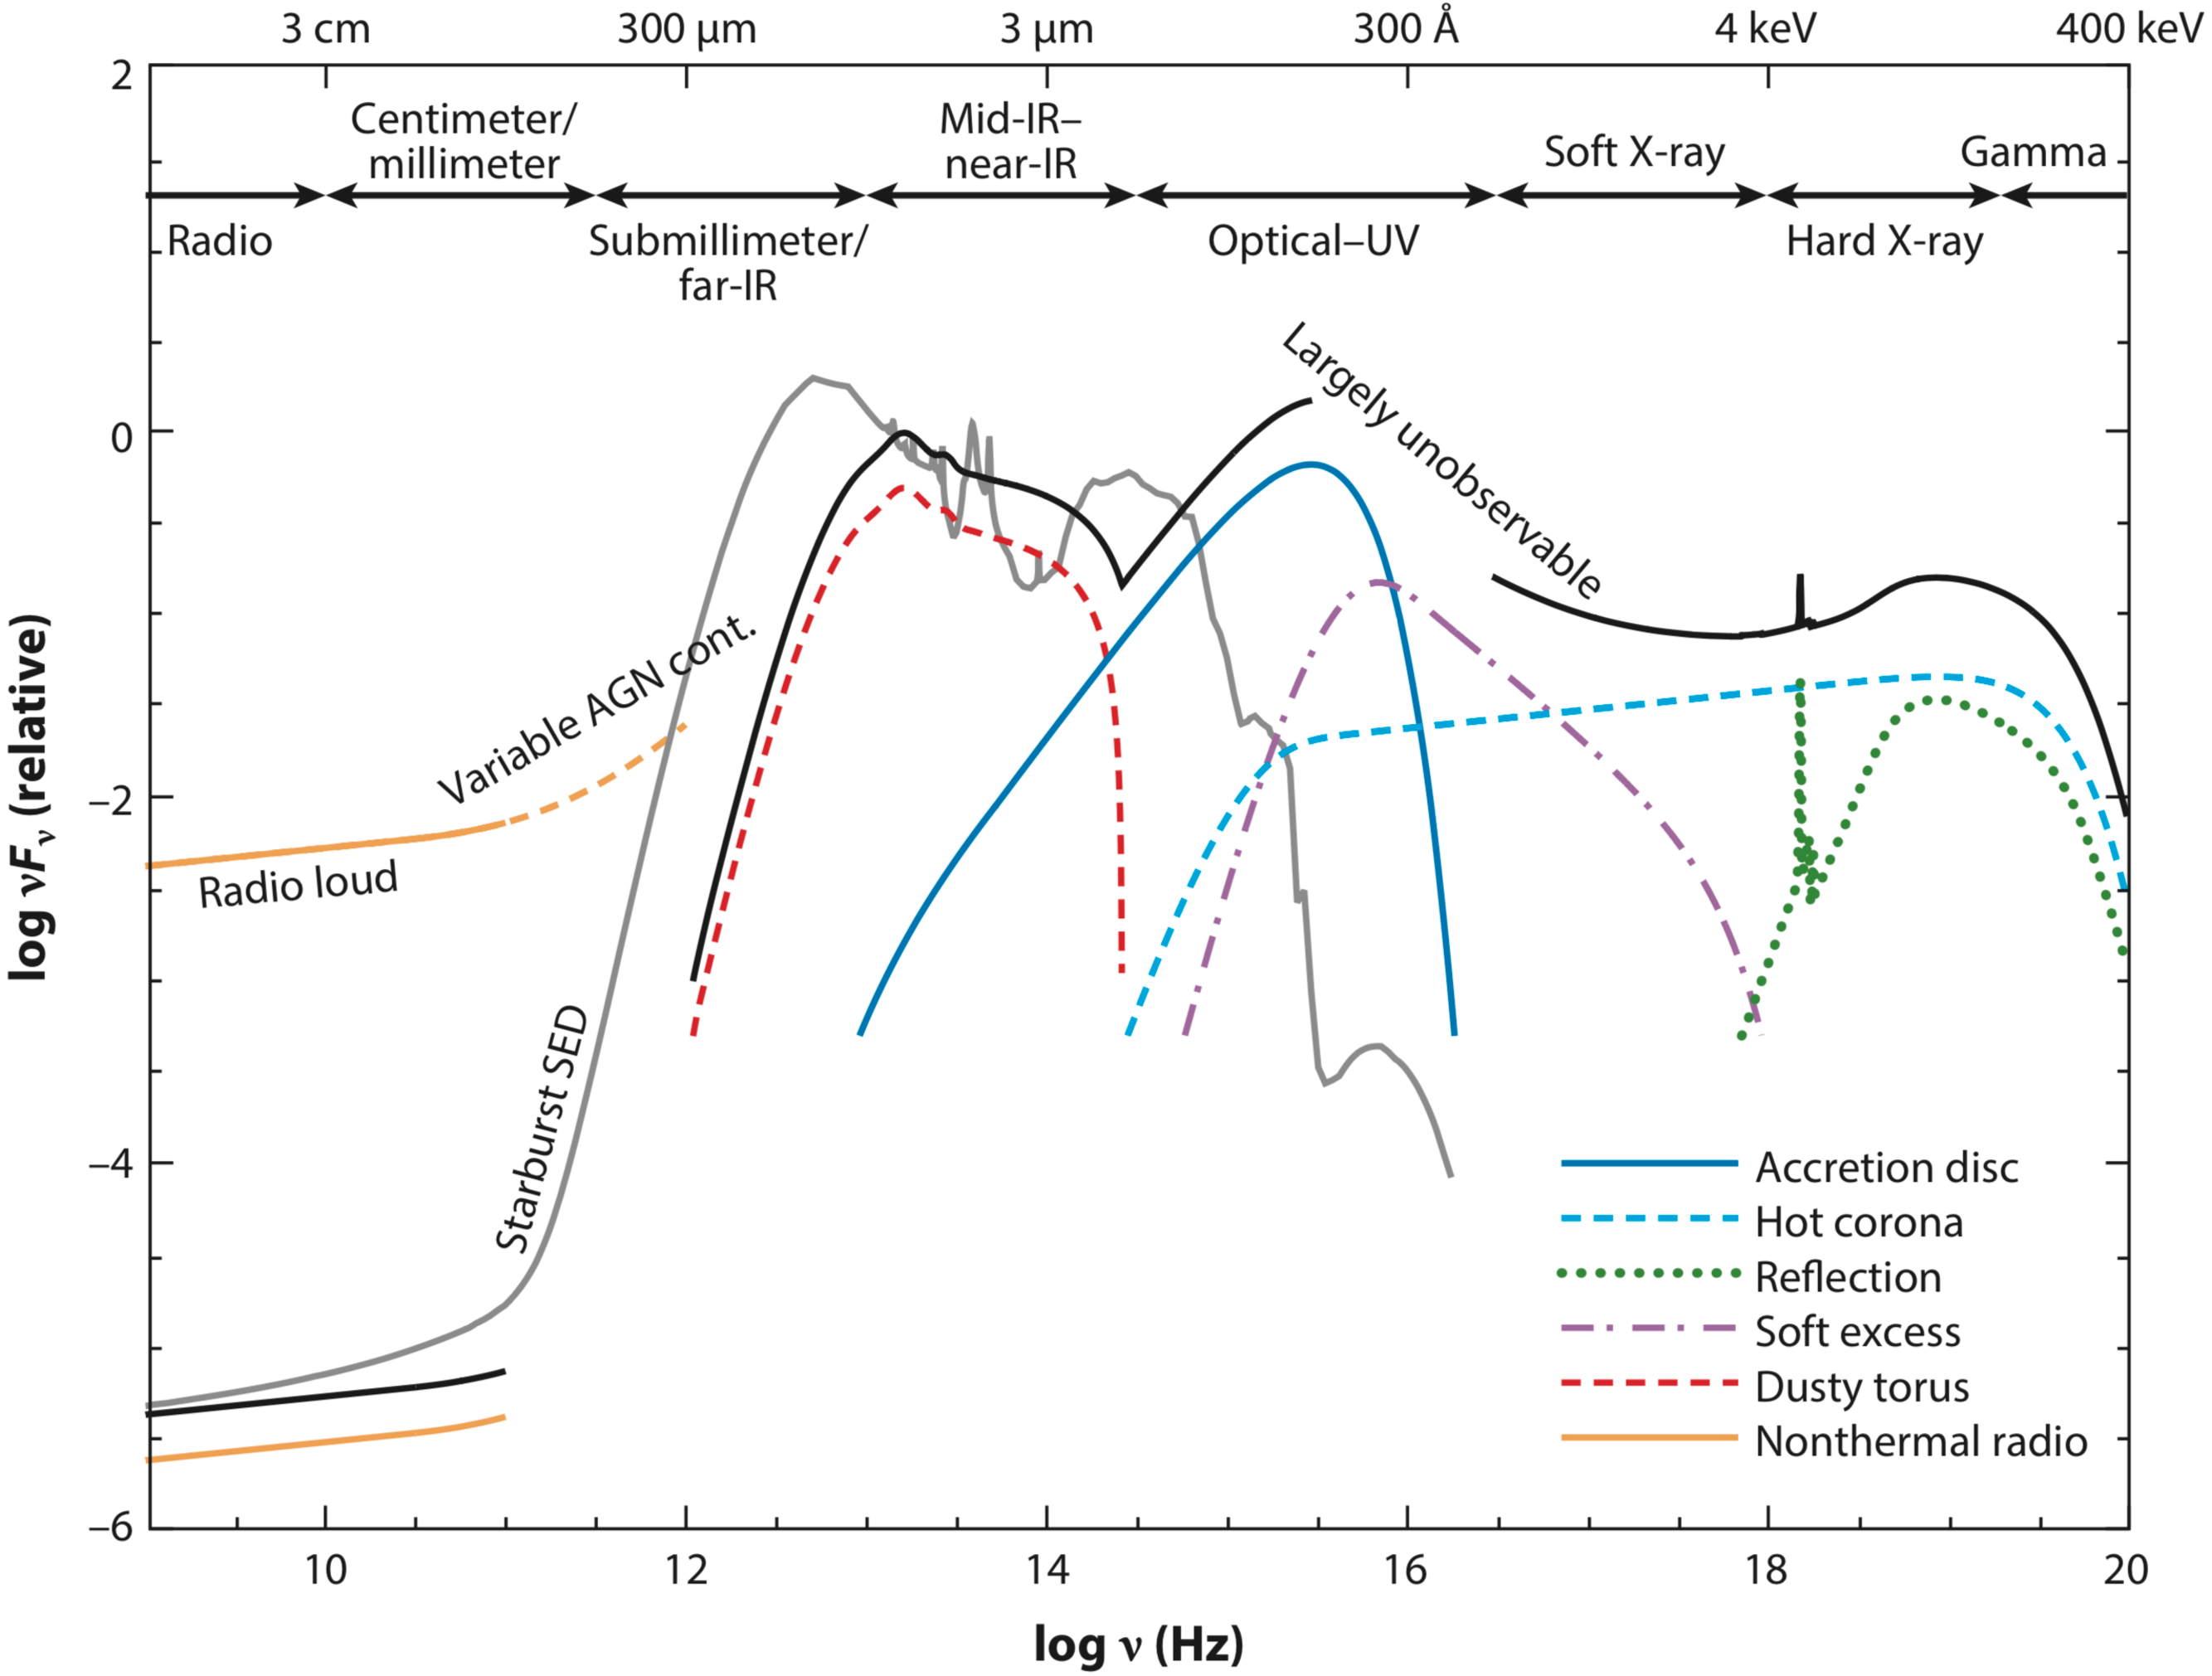
\includegraphics[width=\textwidth]{Figs/Intro/Fig1_Hickox18.pdf}
  \vspace{-30pt}
  \caption{Spectral energy distribution of an AGN. Figure from \citet{2018ARA&A..56..625H}}
    \label{fig:AGN_SED}
\end{center}
\end{figure}

The infalling gas will produce an optically thick disk of material, an accretion disk on a subparsec scale, that will emit thermally because of its own viscosity \citep[e.g.][]{1973A&A....24..337S, 1984ARA&A..22..471R}. The temperature of the gas will increase as it approaches the SMBH and in a typical AGN will range at $T \approx 10^3-10^4 K$ corresponding to a majority of the emission at $\approx 30-300 nm$ (blue line in Fig.~\ref{fig:AGN_SED}).
Around the accretion disk there is a geometrically and optically thick warm–hot dusty and molecular torus which is at a luminosity dependent distance, but within the gravitational influence of the SMBH. It may be considered as the extension of the accretion disk at a distance where dust and molecules can form. The torus is heated by the absorption of shorter-wavelength photons from the accretion disk which it will in turn then re-emit thermally at lower energies, at NIR and MIR wavelengths (red dashed line in Fig.~\ref{fig:AGN_SED}).
Another important source of emission from the black hole is a hot corona above the central part of the accretion disk. This emits in the X-rays through inverse Compton scattering of photons from the accretion disk with relativistic electrons and has a power law shape $N(\nu)\propto \nu^{-\Gamma}$, with $\Gamma=1.8\pm0.2$ (light blue dashed line in Fig.~\ref{fig:AGN_SED}). 
The relativistic electrons in the corona and also in large-scale radio jets can generate synchrotron radiation observable in the radio (yellow line in Fig.~\ref{fig:AGN_SED}).
The primary X-ray continuum can be reprocessed via Compton scattering and photoelectric absorption, thus leading to two important features in the X-ray spectrum: the \kalfa{} emission line and the so-called "Compton-hump", together known as the AGN "reflection" component (green dotted line in Fig.~\ref{fig:AGN_SED}).

In the optical bands, the observed spectrum strongly depends on the inclination of the object. If the dusty torus inclination allows to observe the inner regions we will see emission lines from the broad line region, which is a high density region at about 0.01-0.1pc from the SMBH, close to the accretion disk, where the gas reaches speeds of thousands of km/s. The narrow line region is more external, within the central kiloparsec \citep[e.g.][]{2015MNRAS.454.4452H,2016MNRAS.460..130V}, and is less dense, therefore allowing for forbidden line transitions with lower velocity dispersions, of a few 100s of km/s.

\section{The connection between SFR and BH accretion}
Observational studies and cosmological simulations have revealed a deep interconnection between galaxies and their central supermassive black hole (SMBH): they appear to coevolve and affect each other during their lives.
It has been reported several times that the SMBH mass (M$_{\rm BH}$) correlates with a number of galaxy properties, including bulge mass, stellar velocity dispersion, and starlight concentration as quantified for example by the S\'{e}rsic index. The existence of these relations is not trivial to explain since the SMBH has a very small sphere of influence compared to the galaxy size. While it is relatively easy to explain that gas inflows from the intergalactic medium can feed the star formation during secular processes, it is not easy to understand how the gas loses angular momentum and funnels to the center of the galaxy to feed the SMBH \citep{2019NatAs...3...48S}. %{\bf explicitar que estas relaciones no son obvias, el BH es demasiado pequeño para influenciar directamente la dinámica de la galaxia.} %The relation with the velocity dispersion appears to the most fundamental relation so far \citep[e.g.,][]{2007ApJ...660..267B, 2016MNRAS.460.3119S, 2017MNRAS.466.4029S,2019MNRAS.485.1278S}.
\citet{2007ApJ...660..267B} have seen that a selection effect caused samples of AGN galaxies to be biased to higher velocity dispersions $\sigma$ at a given optical or NIR luminosity $L$. By modeling this bias they were able to show
%By modeling the selection bias that leads to the M$_{\rm BH}$ and velocity dispersion $\sigma$ and M$_{\rm BH}$-galaxy bulge luminosity from optical or NIR bands $L$, \citet{2007ApJ...660..267B} have shown 
that the most fundamental relation is between M$_{\rm BH}-\sigma$ while the relation between M$_{\rm BH}- L$ is a consequence of a relation between $\sigma-L$ and is therefore more biased, as it overpredicts abundances of massive BHs. %{\bf poner un par de oraciones explicando qué es el bias y por qué importa. RC: No entiendo. Si algo està biased significa que està equivocado y para que esté lo màs correcto posible es importante minimizar los bias. Pero eso es algo que cada astrónomo/físico debería saber. A qué te refieres?} 
Also \citet{2017MNRAS.466.4029S} showed that M$_{\rm BH}-\sigma$ is the most fundamental in the scaling relations between black holes and galaxies by studying the residuals of the relations between M$_{\rm BH}$ and $\sigma$, S\'{e}rsic index $n$ and M$_{\rm bulge}$ in SDSS galaxies. Finally, Monte Carlo simulations have shown that a bias can be introduced when dynamically measuring M$_{\rm BH}$: the requirement that the black hole sphere of influence must be resolved to measure black hole masses leads to an increased M$_{\rm BH}-\sigma$ relation of at least a factor three \citep{2016MNRAS.460.3119S}.
%\citet{2007ApJ...660..267B} have modeled the selection bias that leads to the M$_{\rm BH}$ and velocity dispersion $\sigma$ and M$_{\rm BH}$-galaxy bulge luminosity $L$, from optical or NIR bands, and have shown that the most fundamental relation is between M$_{\rm BH}-\sigma$ while the relation between M$_{\rm BH}- L$ is a consequence of a relation between $\sigma-L$ and is therefore more biased, as it predicts more massive BHs at a given luminosity. 
%\citet{2016MNRAS.460.3119S} found through Monte Carlo simulations that a bias can be introduced when dynamically measuring M$_{\rm BH}$: the requirement that the black hole sphere of influence must be resolved to measure black hole masses leads to an increased M$_{\rm BH}-\sigma$ relation of at least a factor three. 
%\citet{2017MNRAS.466.4029S} lead a study in which they studied the residuals of the relations between M$_{\rm BH}$ and $\sigma$, S\'{e}rsic index $n$ and M$_{\rm bulge}$ in SDSS galaxies, and find that $\sigma$ is the most fundamental in the scaling relations between black holes and galaxies.

Interesting insight in this respect has been gained by studying the cosmic star formation rate density (SFRD) and black hole accretion rate densities (BHARD), which are the amount of star formation and black hole accretion per unit of comoving volume at a given redshift. With the fundamental contribution from deep and wide field surveys it has been possible to study them thoroughly and to unveil their evolution.
As can be seen in Fig.~\ref{fig:BHARD}, the BHARD has been determined from IR observations with \emph{Herschel} \citep{2010A&A...518L...1P} and from X-ray observations with XMM-Newton \citep{2001A&A...365L...1J} and Chandra \citep{2000SPIE.4012....2W}. In the IR it was possible to determine the BHARD up to $z\sim3$ \citep{2014MNRAS.439.2736D}, while in the X-rays, thanks to wide and deep surveys it was possible to determine it up to $z\sim 6$ \citep{2018MNRAS.473.2378V}.
%The BHARD has been determined from the IR (up to $z\sim3$, using and \emph{Herschel} data, \citet{2014MNRAS.439.2736D}) and X-ray observations (up to $z\sim 6$ wide and deep surveys from XMM-Newton and Chandra, \citet{2018MNRAS.473.2378V}). 
The history of star formation in galaxies throughout the life of the Universe has been thoroughly constrained in recent years: %it can be estimated from the UV emission of the massive and short-lived stars, but a fraction of it is absorbed by the dust present in the galaxy and then re-emitted in the IR, therefore the SFRD has been studied 
through infrared data with \emph{Herschel}, ultraviolet data with \emph{Galaxy Evolution Explorer} (GALEX) \citep[see][for a review]{2014ARA&A..52..415M} and more recently complemented by sub-mm ALMA data, especially at high redshift up to $z\sim10$ \citep{2020ApJ...902..112B,2020A&A...643A...8G}. %For both SFRD and BHARD the contribution from deep and wide field surveys has been of crucial importance. 
All of these studies have shown that both BHARD and SFRD reach a peak of activity at redshift $z\sim2$ and then decrease to the present epoch \citep{1998MNRAS.293L..49B}.

\begin{figure}
\begin{center}
  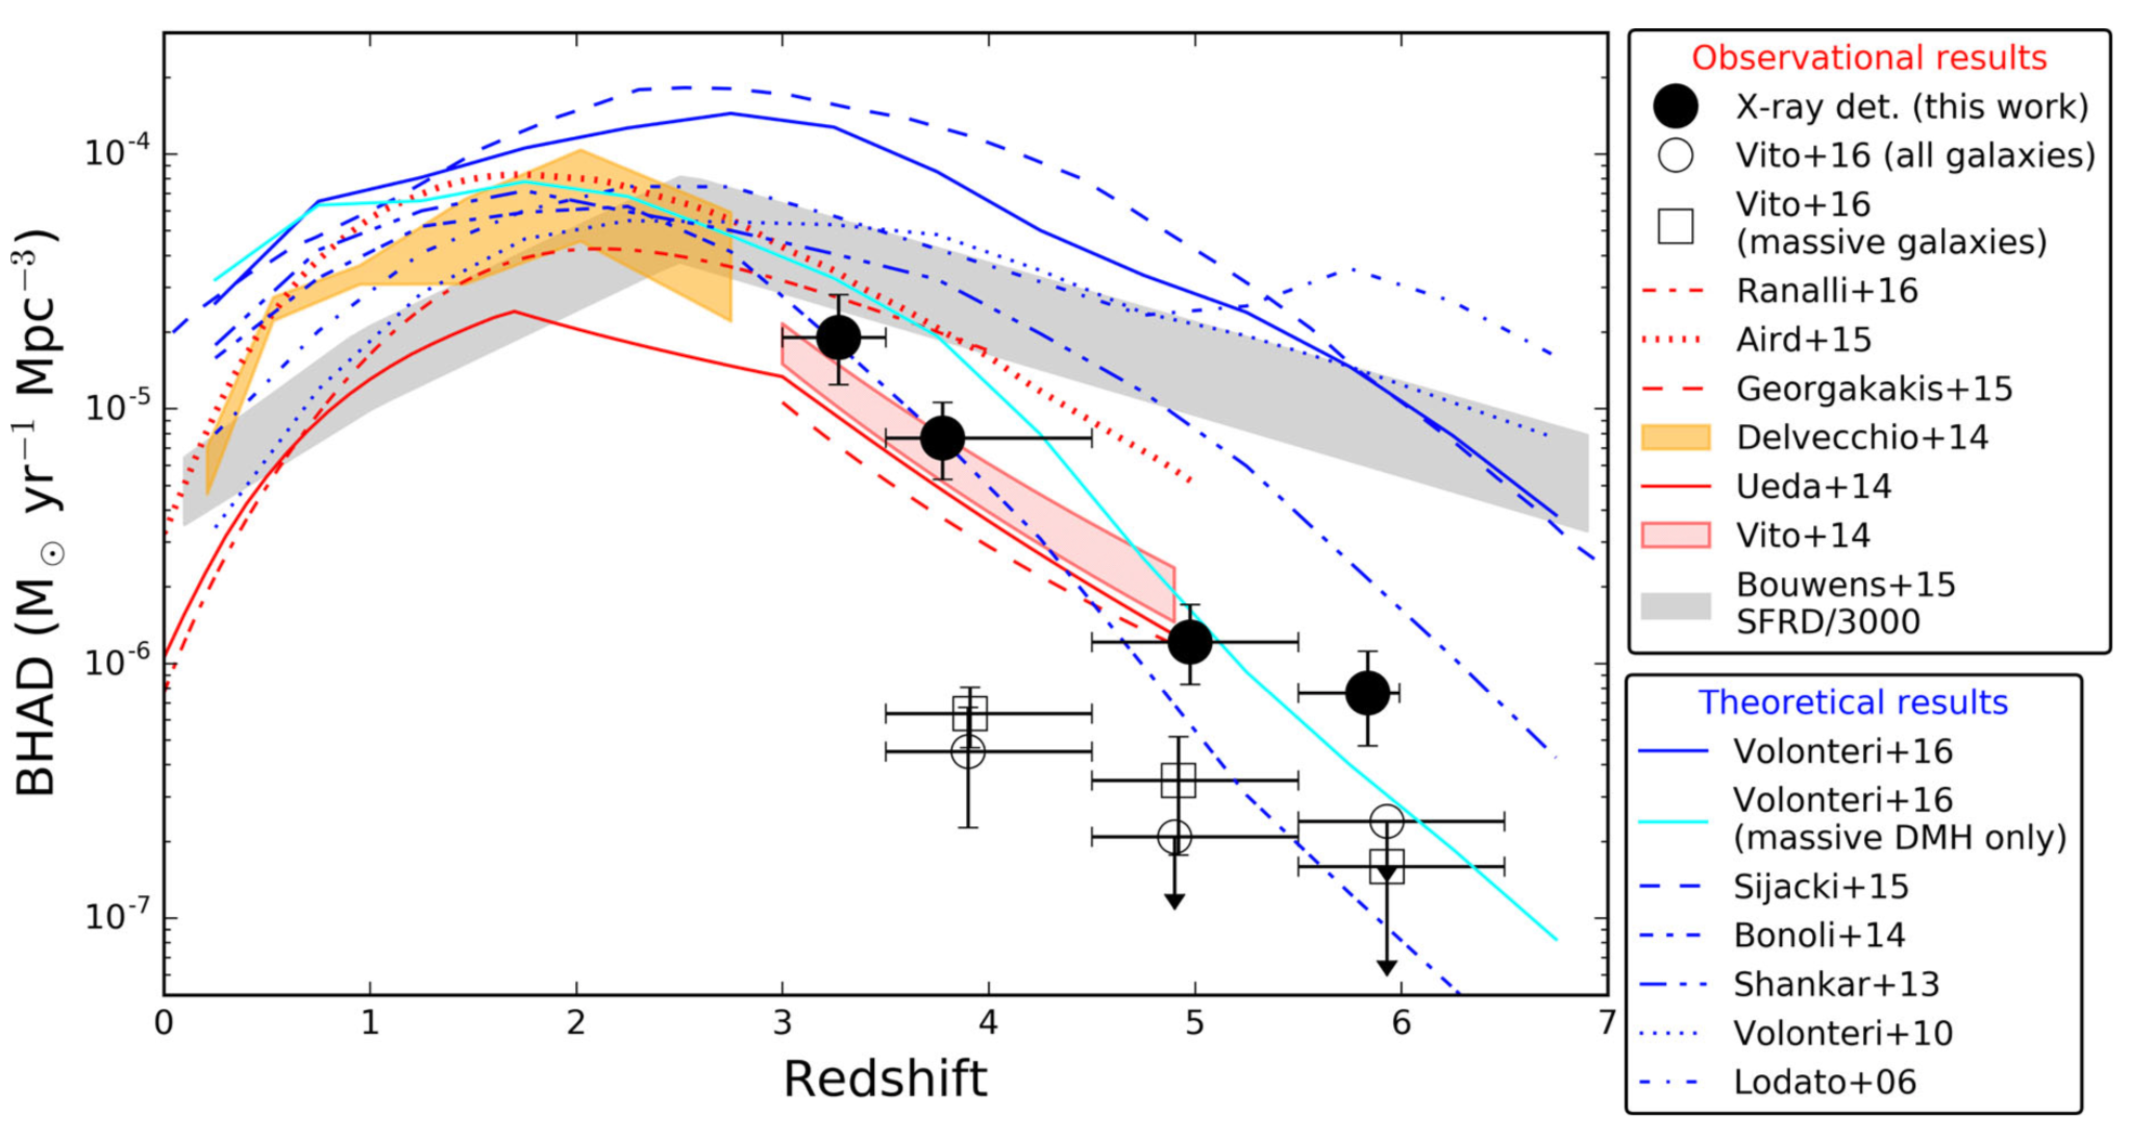
\includegraphics[width=\textwidth]{Figs/Intro/BHARD_Vito18.pdf}
  \vspace{-30pt}
  \caption{BHARD from \citet{2018MNRAS.473.2378V} and other works as reported in the legend. SFRD from \citet{2015ApJ...803...34B} is also reported for comparison purposes.}
    \label{fig:BHARD}
\end{center}
\end{figure}

Additionally, semianalytic models and hydrodynamic simulations show that a self-regulating mechanism, the so called feedback, is required between the star formation and the black hole accretion in order to reproduce local scaling relations, i.e. relations that describe strong trends that are observed between important physical properties of galaxies %{\bf definir scaling relations o al menos recordar lo de arriba y decir relacion entre BH mass y host galaxy properties.}
\citep[see][for a review]{2015ARA&A..53...51S}. Since the pioneering models of galaxy evolution in a cold dark matter framework it was clear that there was an ``overcooling problem'': most of the gas should have cooled and condensed into stars by the present day while it is observed that less than 10\% of it is in the shape of stars, so some suppression of cooling and star formation had to be introduced. This could be as energy released by supernovae \citep{1974MNRAS.169..229L,1978MNRAS.183..341W,1986ApJ...303...39D,1991ApJ...379...52W} and the impact of this phenomenon would be important in regulating star formation in low mass galaxies. On the other hand, luminosity functions predict more high luminosity galaxies in the local universe than we observe, and this might be prevented from happening through feedback from the SMBH as it actively accretes gas %, which is called an active galactic nucleus (AGN)
.%{\bf definir AGN y feedback}
 %AGN also emit in the X-rays, IR and in the radio. The X-ray emission is thought to originate in a corona above the accretion disk by inverse Compton scattering. The IR emission is reprocessed emission from torus and radio from non thermal bremsstrahlung.
The accretion of gas in the BH is an very efficient process, and a fraction of $\approx 5-45\%$, depending on the spin of the black hole \citep[e.g.][]{1963PhRvL..11..237K,1983bhwd.book.....S}, will be emitted as electromagnetic radiation, thereby allowing for very high AGN luminosities.
Simple calculations have shown that when the black hole becomes sufficiently massive ($> 10^7 M_\odot$) its maximum accretion luminosity, the Eddington %{\bf definir Eddington, o decir simplemente maximum accretion luminosity, definir accretion, en realidad, antes de hablar de esto poner qué es un AGN y por qué brilla y por qué podría afectar a su galaxia, ponle un parrafito sobre esto.}
luminosity, becomes high enough that its winds could in principle blow out all of the gas in the entire galaxy \citep{1998A&A...331L...1S}. This feedback mode, called quasar mode, prevents star formation by delivering momentum to the galactic gas and removing it. There is also a radio mode in which the BH is in a low accretion mode and heats the gas, thereby preventing it from collapsing and forming new stars \citep{2017NatAs...1E.165H}.
     
    The decline of the SFRD at low redshift is thought to depend on the decreasing availability of cold gas that is required to form stars and accrete onto black holes \citep[e.g.,][]{2016MNRAS.458L..14F}. Since most of the galaxies lie on the main-sequence of star-forming galaxies, they are the ones that dominate the SFRD evolution \citep{2011ApJ...739L..40R}. The observation of the main sequence at all redshifts and its lack of evolution of the slope, but only an increase of the normalization with redshift, reinforces the belief that most of the SF happens through secular processes \citep{2015A&A...581A..54T, 2015A&A...575A..74S, 2016ApJ...817..118T}: at earlier epochs, galaxies of a given stellar mass were forming more stars than in the local Universe.
    Starburst galaxies are instead a small fraction of star-forming galaxies that are undergoing a stochastic and short-lived episode of considerable galaxy growth, and their SFRs and gas fractions are higher than those on the MS at the same stellar mass, but they cannot be dominating the SFRD because of their low numbers \citep[$\sim2\%$][]{2011ApJ...739L..40R}. 
    Quiescent galaxies, on the other hand, have little star formation but have been shown to evolve from $z\sim1.8,$ where they have significant amounts of dust and gas ($\sim5-10\%$) but their star formation efficiency is low, to the local universe, where they are gas poor \citep{2018NatAs...2..239G}.
    
    Just like star formation, black hole accretion depends on the availability of cold gas. 
    In a classic evolutionary picture predicted by simulations one could have a star forming disk galaxy on the main sequence which undergoes a major merging event \citep{2005Natur.433..604D, 2008ApJS..175..356H}: During the early stages of galaxy merging, gas can efficiently cool and lose angular momentum, eventually feeding black hole growth and central star formation, producing a starburst. The black hole accretion is initially obscured by thick layers of dust, which are then possibly removed by its increasing radiation and momentum feedback, revealing the quasar. Eventually, the gas is consumed, the quasar luminosity fades rapidly, and the star formation episode ceases. This leaves a "red and dead" elliptical galaxy with no or very little star formation or black hole accretion \citep{2004ApJ...600..580G, 2006ApJ...650...42L}. This picture seems to be validated by low redshift (ultra) luminous IR galaxies ((U)LIRGs) which are starburst galaxies often undergoing a major merger event \citep{1996ARA&A..34..749S}, but it doesn't seem to apply to higher redshift galaxies, as many of these don't show signs of a disturbed morphology \citep{2007A&A...468...33E, 2019ApJ...877L..38R}. 
    
    Other theoretical models have predicted pictures of an in situ co-evolution scenario in which SF and black hole accretion are fed by the gas already present in the galaxy and triggered by the early collapse of the host dark matter halos  \citep[e.g.][]{2006ApJ...650...42L, 2011ApJ...742...24L, 2014ApJ...782...69L, 2013ApJ...772..119L,2015ApJ...810...74A, 2016ApJ...833..152M} and/or steady cold gas streams along filaments of the cosmic web  \citep[e.g.][]{2009Natur.457..451D, 2011ApJ...741L..33B}. The accretions are subsequently controlled by self-regulated baryonic physics and in particular by energy feedback from supernovae (SNe) and AGN. In this picture starbursts are gas rich young galaxies, placed to the left of the main sequence (as opposed to \textit{above}). These galaxies then evolve at about a constant SFR while increasing their stellar masses, thus reaching the main sequence locus \citep{2016ApJ...833..152M, 2018ApJ...857...22L}. Additionally \citet{2019MNRAS.482.4454W} find in their semi-analytic models of galaxy formation that not all galaxies in the starburst locus have recently undergone a major merger and that not all the galaxies which have undergone a major merger event result in a starburst.
    Observational results are still not capable to discern between these evolutionary scenarios as deep high resolution data for large statistical samples of starbursts are needed, and only future facilities will be capable to provide them. 
    
    These pictures might suggest that just like the majority of galaxies follow a main-sequence in the SFR-$M_*$ plane, a similar relation between the black hole accretion rate (BHAR) and the $M_*$ might exist: the more massive the galaxy, the higher the availability of inflowing gas for star formation and black hole accretion, which would mean that they both should correlate with stellar mass. In addition, galaxies offset from the main-sequence (starbursts and quiescents), might have a BHAR that varies accordingly with the gas that is typically available in that phase \citep{2019ApJ...877L..38R}. 
    
    In order to search for these potential correlations, many authors have used the X-ray luminosity of galaxies as a proxy of BHAR: X-rays are very energetic photons that are created very close to the central SMBH, and other contaminants in the host galaxies at these wavelengths, for example, emission from stellar processes or binary systems, are usually less powerful and not dominant \citep[e.g.][]{2015A&ARv..23....1B}. Nevertheless, the first studies that traced the instantaneous BHAR with X-ray flux failed at finding any BHAR-M$_*$ relation \citep{2009ApJ...696..396S, 2010A&A...518L..26S, 2012MNRAS.419...95M, 2012A&A...545A..45R, 2015ApJ...806..187A}. A lack of a correlation between SFR and BHAR does not by itself necessarily imply a lack of physical connection. It might arise, for example, from different duty cycles and variabilities that characterize the two processes.  
    Episodes of star formation last for several Gyr, while the SMBH duty cycles are believed to be very short, with accretion episodes of about $10^5$~yr and variability timescales that range from minutes to months.
    
    In order to constrain more robust and reliable BHAR, 
    it is thus necessary to average their growth rate over a long time interval. A very promising technique to achieve this goal consists of stacking X-ray images. Since the BHAR is a stochastic event, stacking large samples of galaxies in a given volume, by grouping them based on optical properties, e.g. the stellar mass,  is equivalent to averaging the growth rate of all galaxies.
    Furthermore stacking allows us to perform studies on mass-complete samples by averaging the count rates of the X-ray images in the optical positions of the galaxies, thus increasing the signal-to-noise ratio, and allowing us to reach fluxes well below the single-source detection threshold of the observations. %{\bf poner en otra oracion que el stacking se hace para galaxias con las mismas caracteristicas opticas, que quede claro que no se está mezclando todo} {\bf pondría esto último primero, que es lo esencial para calcular el crecimiento promedio}
    Previous works indeed searched for a relation between M$_*$ and average BHAR by stacking X-ray images \citep[e.g.,][]{2012ApJ...753L..30M, 2015ApJ...800L..10R, 2017ApJ...842...72Y}, and the probability distribution of specific X-ray luminosity (X-ray luminosity divided by galaxy stellar mass) %{\bf per galaxy? per bin?} 
    with a maximum likelihood approach \citep{2012ApJ...746...90A, 2012MNRAS.427.3103B, 2018MNRAS.475.1887Y} and a Bayesian approach \citep{2018MNRAS.474.1225A}. All studies point toward a positive correlation between the BHAR and the M$_*$ for star-forming galaxies, very similar to the main-sequence of star-forming galaxies, with a slope close to unity, non-negligible redshift evolution, a positive slope for the BHAR-to-SFR ratio as a function of stellar mass, and indications of different behaviors for quiescent and starburst galaxies. 
    Thus far, no study has presented a complete analysis throughout all galaxy life phases by highlighting the evolution of the accretions and the BHAR-to-SFR ratio throughout cosmic time. This is what we present here, in order to understand if the efficiencies of gas conversion in the black hole correspond to those of the star formation, how they vary with time, stellar mass and especially with galaxy life phase. %{\bf pon más explicitamente que interrogante se va a responder con este analisis más completo, aunque sea en varias oraciones. Hay teorías alternativas que se van a probar?} 
    So far, only \citet{2019MNRAS.484.4360A} have shown that the fraction of AGN galaxies is higher below the main-sequence and in starbursts than in the main sequence. %{\bf and SF's?, aquí veremos qué pasa en las otras fases? para restingir qué cosa?}.
        
        We here characterize the evolution of the average BHAR for normal star-forming, quiescent, and starburst galaxies at $0.1<z<3.5$. This redshift interval encompasses the majority of the history of the Universe and contains two crucial epochs in its evolution: the peak of the star formation rate density and BHAR of the Universe at z$\sim$2, and their decline to the local Universe. In Chapter~\ref{ch:observations} 
        we take advantage of the unique depth, area, and wavelength coverage of the COSMOS field, which allows us to select a mass-complete sample with large statistics out to very high redshifts for each galaxy phase. This is particularly important for starbursts, which are rare objects and require a large field in order to be found in good numbers for statistics.
        %We apply the stacking technique to X-ray images from the \textit{Chandra} COSMOS-Legacy survey \citep{2016ApJ...819...62C} and combine the results with the actual X-ray detections in order to estimate the average X-ray luminosity and therefore average BHAR. We compare the evolution of the average BHAR with that of the average SFR. We show that these data confirm and extend previous claims about the evolution of the specific accretions and that the ratio of BHAR to SFR and M$_*$ are correlated. 
        Then in Chapter~\ref{ch:SEM} we use the unique flexibility and simplicity of semi-empirical models to generate mock galaxy catalogs and perform a similar analysis in order to explore the parameters that rule the \LXMS\ by also
        gaining a more comprehensive view of how BHs accrete at different epochs and in different host galaxies.
        
        %explore the parameters that rule evolution of the ${\rm L}_{\rm X}$ (or BHAR) in galaxies across the same redshift range and evolutionary stages.
        
        \section{Gas in active galaxies in the local universe}
        On a different approach, in Chapter \ref{ch:gas_distribution} we study the distribution of the gas generating the X-ray reflected component (green dotted line in Fig.~\ref{fig:AGN_SED}) in a sample of local active galaxies, by assuming that the reflected emission comes from the X-ray continuum and is reprocessed by a dense layer of gas which will produce \kalfa{} emission and damp the variations of the continuum based on its size. We work with a sample of galaxies from Andonie et al. (in prep.) for which we have light curves of both the continuum and \kalfa{} line extracted from Chandra and XMM-Newton archival data. We run Monte Carlo simulations of these light curves, modeled as red noise, in order to determine the size of the reprocessing gas based on the observed smoothing of the \kalfa{} light curves.

\clearchapterpage
%=+=+=+=+=+=+=+=+=+=+=+=+=+=+=+=+=+=+=+=+=+=+=+=+=+=+=+=+=+=+=+=+
%
%%###### CHAPTER 2 #######
%%++++++++++++++++++++++++++++++++++++++++++++++++++++++++++++++++
\chapter{An observational point of view}

%\begin{center}
%  {\it ``If could add an introductionary text here.''}
%  \vspace{1cm}
%\end{center}

We study the coevolution between the black hole accretion rate (BHAR) and the star formation rate (SFR) in different phases of galaxy life: main-sequence star-forming galaxies, quiescent galaxies, and starburst galaxies at different cosmic epochs.
  % methods heading (mandatory)
   We exploited the unique combination of depth and area in the COSMOS field and took advantage of the X-ray data from the {\it Chandra} COSMOS-Legacy survey and the extensive multiwavelength ancillary data presented in the COSMOS2015 catalog, including in particular the UVista Ultra-deep observations.
   These large datasets allowed us to perform an X-ray stacking analysis and combine it with detected sources in a broad redshift interval ($0.1<z<3.5$) with unprecedented statistics for normal star-forming, quiescent, and starburst galaxies. 
   The X-ray luminosity was used to predict the black holeAR, and a similar stacking analysis on far-infrared {\it Herschel} maps was used to measure the corresponding obscured SFR for statistical samples of sources in different redshifts and stellar mass bins.
   
  % results heading (mandatory)
   We focus on the evolution of the average SFR-stellar mass (M$_*$) relation and compare it with the BHAR-M$_*$ relation. This extends previous works that pointed toward the existence of almost linear correlations in both cases. We find that the ratio between BHAR and SFR does not evolve with redshift, although it depends on stellar mass. For the star-forming populations, this dependence on M$_*$ has a logarithmic slope of $\sim0.6$ and for the starburst sample, the slope is $\sim0.4$. These slopes are both at odds with quiescent sources, where the dependence remains constant ($\log(\rm {BHAR}/{\rm SFR})\sim -3.4$).
   %and degree of star formation of the galaxy. 
   By studying the specific BHAR and specific SFR, we find signs of downsizing for M$_*$ and black hole mass (M$_{\rm BH}$) in galaxies in all evolutionary phases. The increase in black hole mass-doubling timescale was particularly fast for quiescents, whose super-massive black holes grew at very early times, while accretion in star-forming and starburst galaxies  continued until more recent times.
  % conclusions heading (optional), leave it empty if necessary 
   Our results support the idea that the same physical processes feed and sustain star formation and black hole accretion in star-forming galaxies while the starburst phase plays a lesser role in driving the growth of the supermassive black holes, especially at high redshift. 
   %Quiescent galaxies appear to be more efficient at growing the black hole than at forming stars. 
   Our integrated estimates of the M$_*$-M$_{\rm BH}$ relation at all redshifts are consistent with independent determinations of the local M$_*$-M$_{\rm BH}$ relation for samples of active galactic nuclei. This adds key evidence that the evolution in the BHAR/SFR is weak and its normalization is relatively lower than that of local dynamical M$_*$-M$_{\rm BH}$ relations.

\section{Data} \label{sec:data}
Our study focuses on the relation between average BHAR, SFR, and $M_*$ across a wide redshift range, from $z=0.1$ to $z=3.5$, and across different evolutionary stages of galaxies: (i) normal star-forming galaxies, which accrete gas secularly to slowly form new stars, and in which the bulk of the cosmic star formation took place; (ii) starburst galaxies, which are a small fraction of all galaxies at all epochs (\citealt[$\sim2\%$]{2011ApJ...739L..40R}; but see also \citealt{2017ApJ...849...45C}) 
and are going through a great burst of star formation that drives them significantly above the main-sequence galaxies on the SFR-M$_*$ plane;
and (iii) quiescent galaxies, which form stars at a very slow pace. 

Star-forming and quiescent galaxies can be easily selected at all redshifts from their emission in the optical/near-infrared (NIR) rest-frame bands, whereas starburst galaxies are heavily obscured in the optical and are therefore more easily identified by the thermal emission from the dust in the far-infrared (FIR). Therefore we selected our samples of star-forming and quiescent galaxies from the catalog by \citet{2016ApJS..224...24L}, which is NIR selected, while we used the FIR-selected catalog by \citet{2013MNRAS.432...23G} to identify starburst galaxies.
%We also use SFR from \citet{2013MNRAS.432...23G}and complement them with stacking on Herschel images and with SFR$_{UV}$(1600\AA). 
For the BHAR we used the catalog by \citet{2016ApJ...819...62C}, obtained from the \textit{Chandra} COSMOS-Legacy program, and complemented it by stacking on their X-ray images. 
We estimated the SFR for star-forming and quiescent galaxies by combining FIR stacking on \textit{Herschel} images and detections with UV luminosity.
We present in this section the catalogs we used for the sample selection and the data we used to estimate the average BHAR and SFR.

\subsection{Optical-NIR catalog}
We selected our sample of star-forming and quiescent galaxies in the COSMOS field \citep{2007ApJS..172....1S} from the COSMOS 2015 catalog \citep{2016ApJS..224...24L}, which uses photometry from UV (\textit{Galex}) to the mid-infrared (MIR, IRAC). This catalog constitutes the UltraVISTA DR2.

The multiwavelength catalog includes UV photometry in the far-UV and near-UV (NUV) bands with the \textit{GALEX} satellite \citep{2007ApJS..172..468Z}; UV/optical photometry in the u*-band from the Canada-France-Hawaii Telescope (CFHT/MegaCam); optical photometry from the COSMOS-20 survey, which is composed of 6 broad bands (B, V, g, r, i, z+), 12 medium bands (IA427, IA464, IA484, IA505, IA527, IA574, IA624, IA679, IA709, IA738, IA767, and IA827), and 2 narrow bands (NB711 and NB816), taken with the Subaru Suprime- Cam \citep{2007ApJS..172....9T, 2015PASJ...67..104T}; new and deeper z$^{++}$ and Y-band data, both taken with the Hyper-Suprime-Cam (HSC) on Subaru; H and $K_s$ NIR photometry obtained with WIRcam/CFHT \citep{2010ApJ...708..202M}, as well as deeper J, H, and $K_s$ imaging obtained with VIRCAM/VISTA UltraVISTA \citep{2012A&A...544A.156M} in the central 1.5~deg$^2$ of the COSMOS field (the coverage by
UltraVISTA is not homogeneous, with alternating "deep" and "ultradeep" stripes that reach depths of 24 and 24.7 in $K_S$-band, respectively); NIR data from IRAC, as part of the SPLASH COSMOS
, together with S-COSMOS \citep{2007ApJS..172...86S}; MIR and FIR data with \textit{Spitzer} IRAC and MIPS (Multi-band Imaging Photometer), from the \textit{Spitzer} Extended Mission Deep Survey and the \textit{Spitzer}-Candels survey \citep{2015ApJS..218...33A} data, among others; FIR from the \textit{Herschel} PACS and SPIRE instruments, taken as part of the PACS Evolutionary Probe (PEP) guaranteed-time key program \citep{2011A&A...532A..90L}, the largest field of the program, observed for about 200 h to a 3$\sigma$ depth at 160 $\mu m$ of 10.2 $mJy$ and at 100 $\mu m$ $\sim$5 $mJy$.


The point spread function (PSF) of the VISTA bands was estimated in each photometric band by modeling isolated known stars from the COSMOS ACS/HST catalog \citep{2007ApJS..172..196K, 2007ApJS..172..219L} with the PSFEX tool \citep{2013ascl.soft01001B}; 
The target PSF was chosen in order to minimize the applied convolutions, and it is the desired PSF of all bands after homogenization.
The required convolution kernel was calculated in each band by finding the kernel that minimizes the difference between the target PSF and the convolution product of this kernel with the current PSF. The images were then convolved with this kernel.

Then, a $\chi^2$ detection image \citep{1999AJ....117...68S}, produced by combining NIR images of UltraVISTA ($YJHK_S$) with the optical $z^{++}$-band data from Subaru, was used to identify objects; the photometry for these objects in the other bands was obtained by running SEXTRACTOR in dual-image mode. Fluxes were extracted from 2'' to 3'' diameter apertures on PSF-homogenized images in each band, except for a few cases: for \textit{GALEX}, the fluxes were measured using a PSF fitting method with the u*-band image used as a prior, and for the SPLASH IRAC imaging, the IRACLEAN tool \citep{2012ApJS..203...23H} was used to derive the photometry using the UltraVISTA $zYJHK_s$ $\chi^2$ image as a prior.
Photometry at 24 $\mu$m was obtained from the COSMOS MIPS-selected band-merged catalog \citep{2009ApJ...703..222L}. Far-IR photometry is provided by \textit{Herschel} PACS \citep[PEP guaranteed-time program,][]{2011A&A...532A..90L} and SPIRE \citep[HERMES consortium,][]{2012MNRAS.424.1614O} at 100, 160, 250, 350, and 500 $\mu$m.

The \citet{2016ApJS..224...24L} catalog provides secondary products as well, including photometric redshifts, stellar masses, and star formation rates. In particular, photometric redshifts were computed with \emph{Le Phare} \citep{2002MNRAS.329..355A, 2006A&A...457..841I} with the same method as was used in \citet{2013A&A...556A..55I}: the spectral energy distributions (SED) in 3 arcsec  apertures were fit to a set of 31 templates, including spiral and elliptical galaxies from \citet{2007ApJ...663...81P} and a set of 12 templates of young blue star-forming galaxies, produced using the models of \citet{2003MNRAS.344.1000B}. Photometric redshifts for objects that are detected in X-rays were instead taken from \citet{2016ApJ...817...34M}, who applied a set of templates that is more suitable for X-ray detected galaxies, in which the central black hole might significantly affect the UV/optical photometry (see section~\ref{ssec:Xray}). Photometric redshift precision was characterized by comparing it with spectroscopic samples from the COSMOS spectroscopic master catalog (M. Salvato et al., in preparation).% - CERCANDO HO TROVATO QUESTO. G. Hasinger+18, è l'unico paper di spettroscopia in cosmos con lei: http://iopscience.iop.org/article/10.3847/1538-4357/aabacf/pdf}

Stellar masses were derived using \emph{Le Phare}, with the same method as presented in \citet{2015A&A...579A...2I}: a \citet{2003PASP..115..763C} initial mass function was assumed, and the photometry was fit with a library of synthetic spectra generated using the stellar population synthesis model of \citet{2003MNRAS.344.1000B}, assuming both exponentially declining star formation histories (SFH) and delayed SFH ($\tau^{-2}te^{-t/\tau}$), assuming two different metallicities (solar and half-solar). Emission lines were added following the prescription in \citet{2009ApJ...690.1236I} together with two attenuation curves (the starburst curve of \citealt{2000ApJ...533..682C} and a curve with a slope $\lambda^{0.9}$ from Appendix A of \citealt{2013A&A...558A..67A}). The E(B - V) values were allowed to vary in a range between 0 and 0.7. The masses were then obtained as the median of the marginalized probability distribution function (PDF).

\subsection{IR data}\label{ssec:IRdata}
We selected the starburst galaxies sample for this work from a FIR-selected catalog. In particular, we used the \citet{2013MNRAS.432...23G} catalog, which is selected from PACS/\textit{Herschel} PEP observations in the COSMOS field. This catalog was also matched with the deep 24 \textmu m imaging of \citet{2009ApJ...703..222L}, with the HerMES extragalactic survey \citep{2012MNRAS.424.1614O} observed with SPIRE at 250, 350, and 500~\textmu m in the same fields that were covered by PEP and with the IRAC-based catalog of \citet{2010ApJ...709..644I}, including optical and NIR photometry and photometric redshifts.

%omogeneizzazione psf - estrazione sorgenti\\
\citet{2013MNRAS.432...23G}) used as reference the blind catalogs at 100 and 160 \textmu m from \citet{2010A&A...518L..30B,2011A&A...532A..49B}, selected down to the $3\sigma$ level, which in COSMOS contain 5355 and 5105 sources at 100 and 160 \textmu m, respectively. Then they associated their sources with the ancillary catalogs by means of a multiband likelihood ratio technique \citep{1992MNRAS.259..413S,2001Ap&SS.276..957C}, starting from the longest available wavelength (160 \textmu m, PACS) and progressively matching 100 \textmu m (PACS) and 24 \textmu m (MIPS). Their final catalog consists of 4110 and 4118 sources at 100 and 160 \textmu m, respectively. Spectroscopic or photometric redshifts are available for 3817 and 3849 of their sources, respectively, which they used for the SED fitting in order to estimate the FIR luminosity function.

Stellar masses were obtained by fitting the broadband SED with a modified version of MAGPHYS \citep*{2008MNRAS.388.1595D}, which  simultaneously fits the broadband UV-to-FIR observed SED of each object and ensures an energy balance between the absorbed UV light and the light that is reemitted in the FIR regime. The redshift for each object was fixed to the spectroscopic redshift when available or else to the photometric redshift; then the SED was fit to a best-fit model that we selected from a library built by combining different SFH, metallicities, and dust contents. Each SFH is the combination of an exponentially declining SFR model, to which random bursts of star formation are superimposed \citep[see][]{2008MNRAS.388.1595D, 2010MNRAS.403.1894D}. The emission of a possible AGN component was taken into account using a modified version of the MAGPHYS code \citep[SED3FIT,][]{2013A&A...551A.100B}, which adds a torus component to the modeled SED emission by combining the \citet{2008MNRAS.388.1595D} original code with the \citet*{2006MNRAS.366..767F} AGN torus library \citep[see also][]{2012MNRAS.426..120F}.

In order to estimate the SFR of their sample, \citet{2013MNRAS.432...23G} calculated an SED using all the available multiwavelength data by performing a $\chi^2$ fit using the \emph{Le Phare} code \citep{2002MNRAS.329..355A, 2006A&A...457..841I} with the semiempirical template library of \citet{2007ApJ...663...81P}, which is representative of different classes of IR galaxies and AGN. They also added some modified templates in the FIR to better reproduce the observed {Herschel} data \citep[see][]{2010A&A...518L..27G}, and three starburst templates from \citet{2009ApJ...692..556R}.
Then they integrated the best-fitting SED of each source over $8\leq \lambda_{rest}\leq1000$~\textmu m to derive the total IR luminosities (L$_{\rm IR}$ = L[8--1000 \textmu m]) in 11 redshift bins (0.0--0.3, 0.3--0.45, 0.45--.6, 0.6--0.8, 0.8--1.0, 1.0--1.2, 1.2--1.7, 1.7--2.0, 2.0--2.5, 2.5--3.0, and 3.0--4.2). 
Finally, they estimated the SFR$_{\rm IR}$ for all these sources from the total IR luminosity after subtracting the AGN contribution and using the \citet{1998ARA&A..36..189K} relation \citep[see also][for more details]{2015MNRAS.451.3419G}.

\subsection{X-ray data} \label{ssec:Xray}
We used X-ray data from the \textit{Chandra} COSMOS Legacy Survey \citep[COSMOS-Legacy,][]{2016ApJ...819...62C}, a 4.6 Ms \textit{Chandra} program that combines new observations obtained during \textit{Chandra} Cycle 14 with the previous C-COSMOS Survey, allowing the X-ray data to uniformly cover the whole 2.2 deg$^2$ of the COSMOS field. The limiting fluxes are  $2.2 \times 10^{-16}, 1.5 \times 10^{-15}$, and $8.9 \times 10^{-16} \um{erg}\ump{cm}{-2} \ump{s}{-1}$ in the 0.5--2, 2--10, and 0.5--10~keV bands, respectively.

The optical counterparts to the X-ray COSMOS-Legacy sources are available in \citet{2016ApJ...817...34M}. This was obtained by using the maximum likelihood ratio technique \citep[e.g.,][]{1992MNRAS.259..413S, 2005A&A...432...69B, 2012ApJS..201...30C} by matching X-ray sources to three separate bands: i-band data from \citet{2009ApJ...690.1236I}, $K_s$-band data using UltraVISTA DR2, and IRAC 3.6 micron using either SPLASH or \citet{2007ApJS..172...86S}
sources from the \citet{2016ApJS..224...24L} catalog in the UltraVISTA field.
Optical counterparts were cross-correlated with the master spectroscopic catalog (Salvato et al. in prep), which contains spectroscopic redshifts from numerous observing campaigns and instruments. For the sources for which no spectroscopic redshift is available, a photometric redshift was provided that we obtained by following the same procedure as in \citet{2011ApJ...742...61S}. %We show on Table~\ref{table:n_gal} the number of sources in our sample with an X-ray counterpart (detections) and the not detected ones, which were stacked (see section~\ref{sec:stacking} for more details).

%-------------------------------------------------------------
%                                    One column rotated figure
%-------------------------------------------------------------
   \begin{figure*}
   \centering
   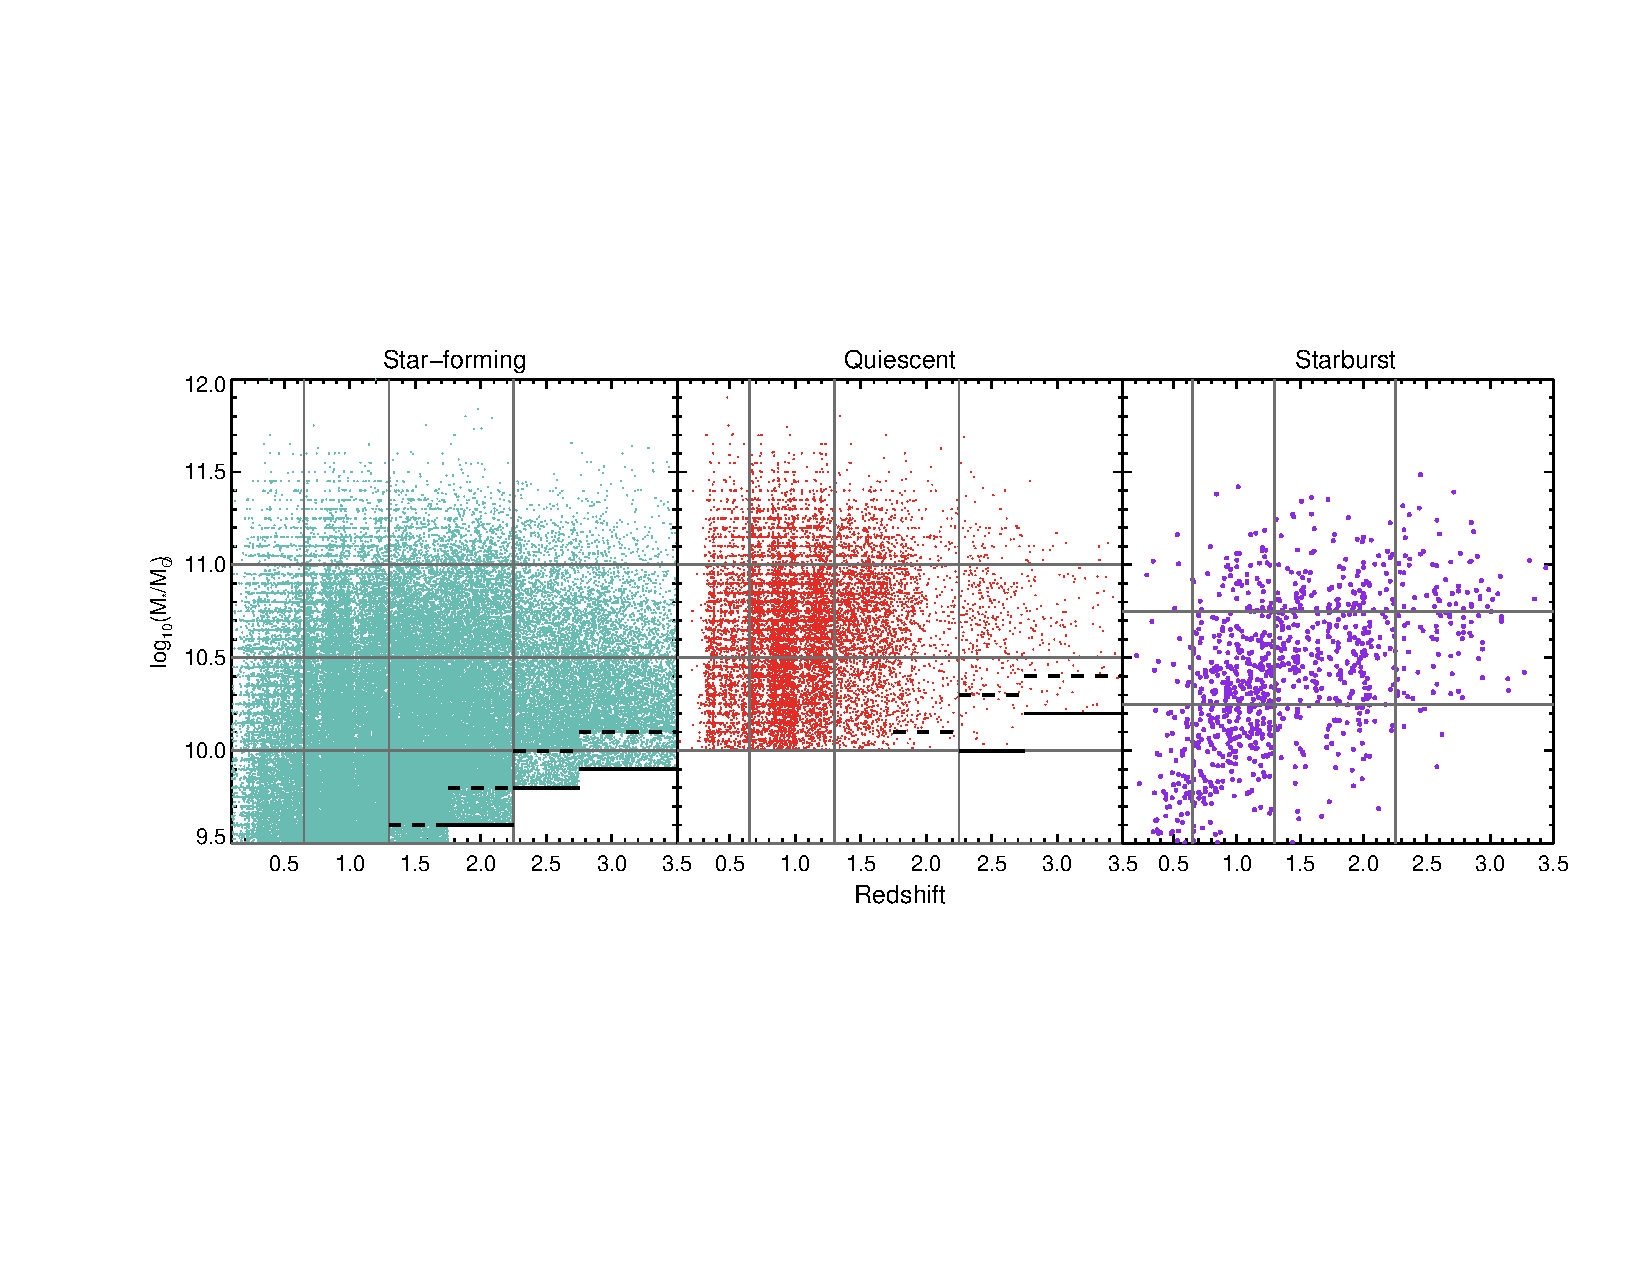
\includegraphics[trim={2cm 6cm 1cm 5.5cm}, clip, width=\textwidth]{Figs/M_vs_z_separate.pdf}
    \caption{ Stellar mass of our sample of galaxies shown as a function of redshift. Star-forming and quiescent galaxies are selected from \citet{2016ApJS..224...24L} (green and red data points in the left and central panel, respectively), while the starbursts are selected from \citet{2013MNRAS.432...23G} (violet data points in the right panel).
                        The solid and dashed black lines are the mass completeness thresholds are for UVista
                        deep and ultradeep stripes from \citet{2016ApJS..224...24L} for star-forming and
                        quiescent galaxies. For starburst galaxies we considered as mass incomplete the low-mass
                        bins (9.50<$\log_{10}($M$_\sun$/M$_*)$<10.25) at $z>1.30$.
                The solid gray horizontal and vertical lines show the limits of our mass and redshift bins.
                }
         \label{fig:M_vs_z}
   \end{figure*}

%--------------------------------------------------------------------

%-----------------------------------------------------------------
\section{Sample selection} \label{sec:sample}
We selected a mass-complete sample from \citet{2016ApJS..224...24L} by limiting our selection to the area that is covered by the UltraVISTA-DR2 observations (1.5 deg$^2$) in the redshift interval $0.1<z<3.5$. In order to separate star-forming from quiescent galaxies, we used the classification from \citet{2016ApJS..224...24L}, which  is based on the rest-frame NUV$ - r / r - J$ color-color diagram as in \citet{2013A&A...556A..55I}. It allows separating dust-obscured galaxies from older stellar populations. In this diagram, galaxies with colors NUV$ - r>3 (r-J)+1$ and NUV$ - r > 3.1$ are classified as quiescent.

We selected starburst galaxies from the \citet{2013MNRAS.432...23G} catalog in the same redshift interval down to M$_*\sim 10^{9.5} M_\sun$. Again, we chose this catalog because it is FIR selected, that is, selected based on the specific star formation rate (at least to a first approximation), and includes SFR$_{\rm IR}$ estimates, which allowed us to robustly estimate the SFR of highly star-forming galaxies that are heavily obscured. 
Based on Fig. 15 of \citet{2013MNRAS.432...23G}, above $z\sim1.3$ we probably miss the low-SFR starburst sources, therefore we decided to show these data points as upper limits.
 The starburst galaxies were selected to have an SFR that is at least four times higher than the SFR of a typical main-sequence galaxy with a similar stellar mass and redshift, which is our definition of starburst galaxy.
For the purpose of their selection, we considered the parameterization of the main-sequence from \citet{2015A&A...575A..74S} and obtained the relation
\begin{multline}  \label{eq:SFR_thresh}
\textrm{SFR}_{IR}^{SB} \geq 4 \times \textrm{SFR}_{MS}(z_{ave},M_*)=\\
=4 \times \left[m-m_0+a_0r-a_1[\max(0,m-m_1-a_2r)]^2 \right],
\end{multline}
where SFR$_{IR}^{SB}$ is the star formation rate of a starburst galaxy obtained from its IR luminosity, $r=\log_{10}(1+z)$, $m=\log_{10}(M_*/10^9M_\cdot)$, and the parameters $m_0=0.5$, $m_1=0.36$, $a_0=1.5,$ and $a_1=0.3$.
We used SFR$_{IR}^{SB}$, M$_*$ , and $z$ from the \citet{2013MNRAS.432...23G} catalog.
We matched the starburst sample with the catalog of star-forming and passive galaxies that was previously color-color selected from \citet{2016ApJS..224...24L}, using a 3.5'' association radius in order to exclude the starburst galaxies from our star-forming and quiescent selection. For a distance greater than 2'' we only accepted matches that have a $\Delta z = |\, z_{\rm Gruppioni} - z_{\rm Laigle} \,|<0.3$, allowing us to include seven more starburst galaxies in our sample.
We compared the stellar masses of the starburst sample (derived from MAGPHYS) with their stellar masses from \citet{2016ApJS..224...24L} (derived from \emph{Le Phare}) in each of the redshift bins and found that they lie along the 1:1 relation with increasing scatter with redshift (RMS ranging from 0.18 dex at low z to 0.35 dex at high-z), but with no offset (the median of the difference of the masses is about $10^{-2}$). From the cross-match we find that 965 color-selected star-forming galaxies are IR-classified as starbursts (this is expected because the NUV$ - r / r - J$ diagram does not have a starburst area) and 28 color-selected quiescents are IR starbursts. We moved 1494 galaxies that are $24\mu m$ MIPS/\textit{Spitzer} detected from our quiescent selection to the star-forming galaxy sample because the IR emission indicates that a certain amount of optically hidden star formation is ongoing. For the X-ray detected star-forming and quiescent galaxies we used the redshift included in \citet{2016ApJ...817...34M}. We have a final number of 83,904 star-forming, 12,839 quiescent, and 1,003 starburst galaxies.

We further divided the sample into four redshift bins: 0.1<z<0.65, 0.65<z<1.3, 1.3<z<2.25, and 2.25<z<3.5.

Every redshift bin was chosen with the purpose of including a sufficient number of galaxies (see Table~\ref{table:n_gal}), and then the galaxy sample of each redshift bin was divided into mass bins. Our final sample is shown in Fig.~\ref{fig:M_vs_z} together with the mass-completeness thresholds from \citet{2016ApJS..224...24L} for star-forming and quiescent galaxies and the limits of our stellar mass and redshift bins. 

\section{Method} \label{sec:method}
The aim of this paper is to study the average BHAR for galaxies with different star formation activities, from passive galaxies to starbursts, at different cosmic epochs and at different stellar masses. Because AGN activity is a stochastic event, as the AGN duty cycle is short compared to the star formation episodes in galaxies, it is unlikely that a galaxy has been observed at the peak of its black hole accretion. This means that if we limited the analysis to bright X-ray galaxies, we would obtain a biased view of the average AGN activity in
galaxies. For this reason, we complement X-ray individual detections with the stacking analysis on \textit{Chandra} X-ray images for nondetected galaxies. 

\subsection{X-ray stacking analysis} \label{sec:stacking}
In order to estimate the average X-ray luminosity for each mass and redshift subsample, we followed the same method as in \citet{2015ApJ...800L..10R}. We used individual X-ray detections from the COSMOS-Legacy catalog \citep{2016ApJ...819...62C} when possible, taking advantage of the match between optical and X-ray sources performed by \citet{2016ApJ...817...34M} (see section \ref{ssec:Xray}). For the non-X-ray detected sources we performed stacking on the same images using the CSTACK tool v4.32\footnote{\url{http://cstack.ucsd.edu/cstack} or \url{http://lambic.astrosen.unam.mx/cstack/} developed by Takamitsu Miyaji.}  \citep{2008HEAD...10.0401M}.

We propagated the probability distributions of count rates with Monte Carlo simulations. We focused on the 2-7~keV band and took advantage of the CSTACK bootstrap output. We simulated it $10^6$~times by interpolating the inverted cumulative distribution function of the bootstrap probability distribution.
For X-ray detections, we instead assumed a Gaussian probability distribution and a $\sigma$ equal to the error on the count rate from the catalog when available. Alternatively, we set the error on the detection to $\sigma=0.25 \times CR(2-7\um{keV}).$  Count-rate distributions from the stacking and detections were converted into standard flux in the $2-10\um{keV}$ band through the WebPIMMS\footnote{\url{http://cxc.harvard.edu/toolkit/pimms.jsp}} conversion factor obtained for \textit{Chandra} cycle 14
by assuming a power-law spectrum for the AGN with photon index $\Gamma$= 1.8 and galactic hydrogen absorption \citep[N$_H=2.6\times 10^{20} \ump{cm}{-2}$,][]{2005A&A...440..775K}.
This value of the photon index $\Gamma$ is compatible with the cosmic X-ray background according to \citet{2019ApJ...871..240A} for cutoff energies E$_c<100\um{keV}$.
We converted fluxes into rest-frame with a K-correction with the shape of $K_{corr}=(1+z)^{\Gamma-2}$ , where $z$ is the average redshift of each subsample and $\Gamma$ is the photon index just introduced.

Because we search for a global average X-ray measurement by combining detections and non-detections in each redshift and mass bin, we applied the following equation to all the fluxes in the probability distribution of each detection and the stacking:
\begin{equation}  \label{eq:F_ave}
\centering
F_\text{ave}=\frac{\sum_{j=1}^{n_{\text{detected}}}F_{j,\text{detected}}+n_{\text{stacked}}\cdot F_{\text{stacked}}}{n_{\text{detected}}+n_{\text{stacked}}}
,\end{equation}
where in each redshift and mass bin, $n_{\text{detected}}$ is the number of detections, $F_{j,detected}$ is the flux of each detection, $n_{\text{stacked}}$ is the number of undetected objects that were therefore stacked, and $F_{stacked}$ is the total flux from the stacked objects. This returns a probability distribution of rest-frame flux for each redshift and mass bin. We show in Table \ref{table:n_gal} the number of stacked and detected galaxies.

%-------------------------------------- Two column figure (place early!)
   \begin{figure*}
   \centering
   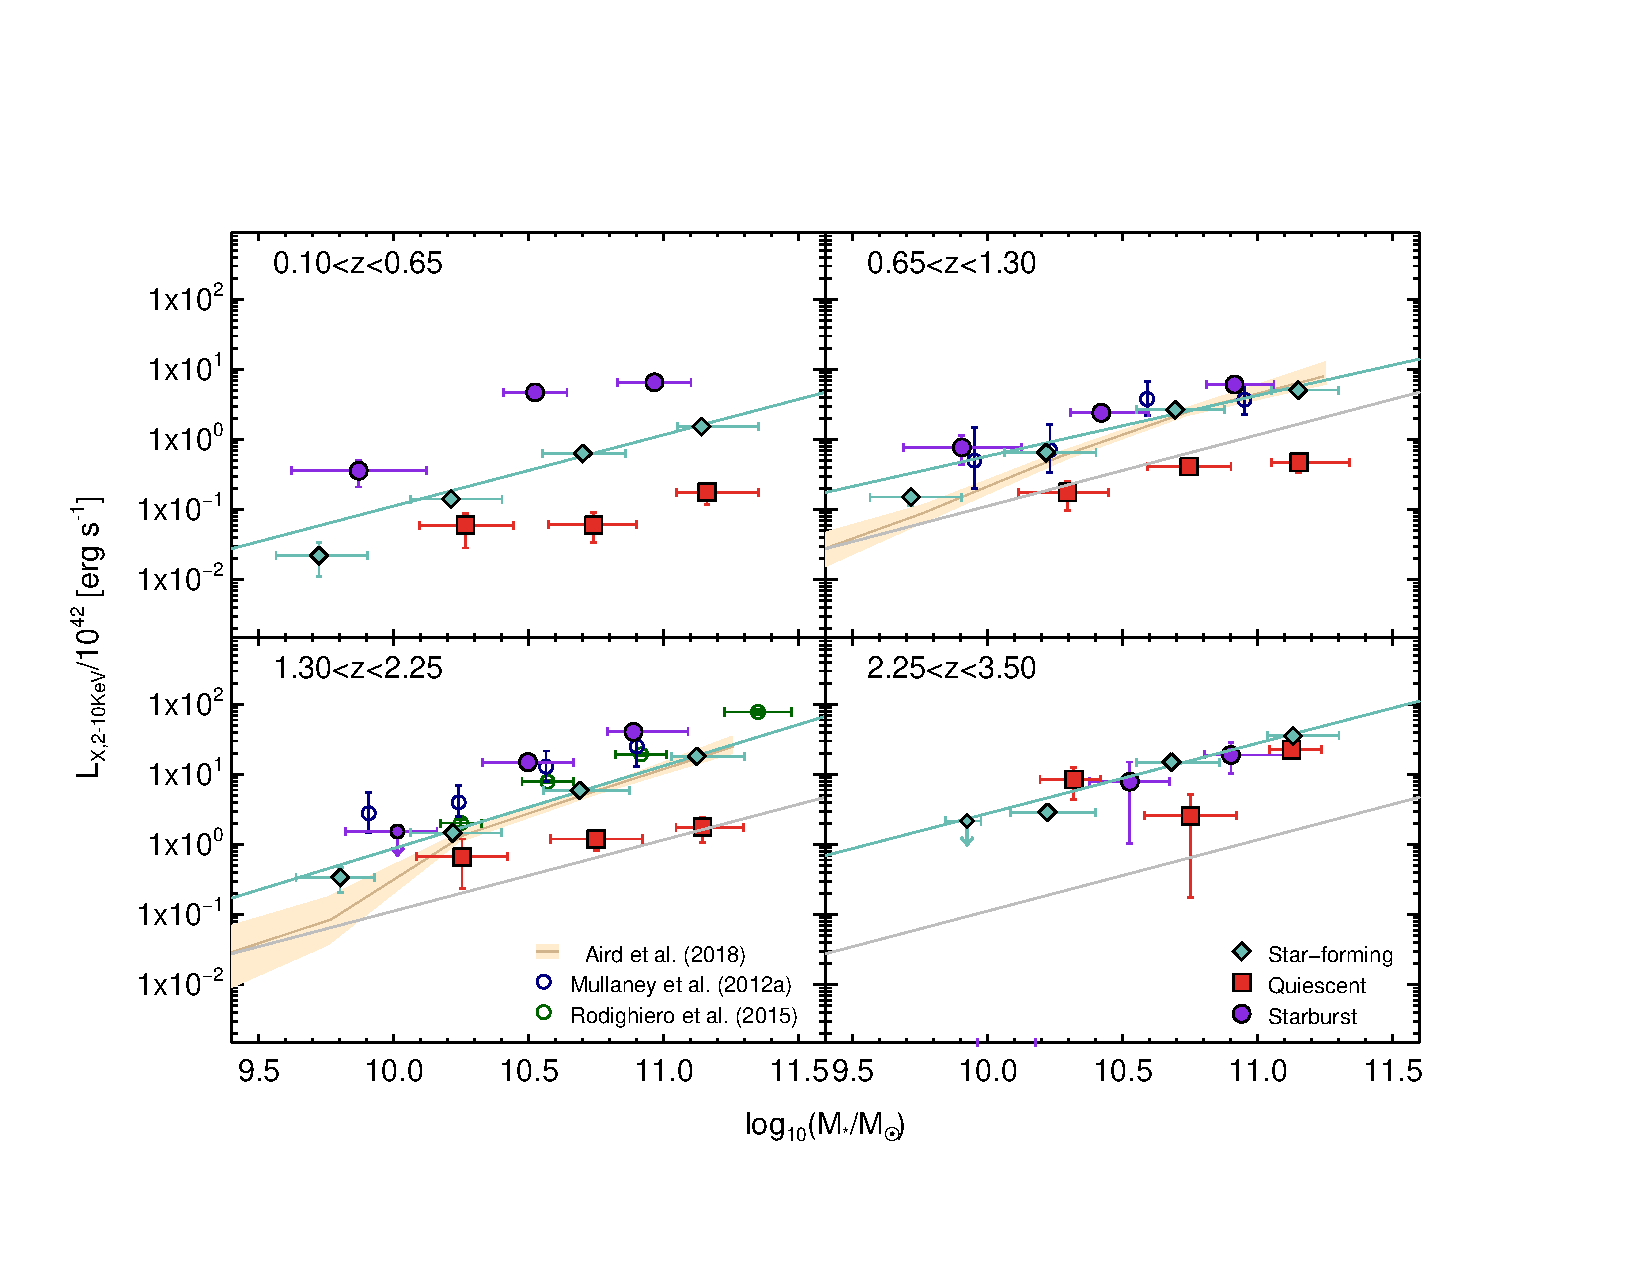
\includegraphics[trim={1cm 2cm 2.5cm 3cm}, clip,width=\textwidth]{Figs/L_X.pdf}
      \caption{X-ray luminosity in the 2-10~keV band for our sample as a function of stellar mass. Each panel represents one of the four redshift bins that we considered. The light green diamonds represent the normal star-forming sample, the red squares represent the quiescent sample, and the violet circles represent the starburst sample. The data points represent the median value of the stellar mass and the X-ray luminosity. Vertical error bars represent the 5th and 95th percentile (90\% confidence interval) of the distributions, while horizontal error bars correspond to $1~\sigma$. We show an upper limit (the 95th percentile) for the data points whose X-ray luminosity 5th percentile is compatible with zero and for starburst galaxies at high redshift and low mass, where our sample is incomplete.
      The light green continuous line is the best fit for the star-forming galaxy data points at each redshift, while the gray line shows the best fit in the lowest redshift bin, shown for comparison purposes.  
      We also report data points from \citet{2012ApJ...753L..30M} at an average redshift of $z=1,2$ (open dark blue circles, \citet{2015ApJ...800L..10R} at an average redshift of $z=2$ (open green circles) and \citet{2018MNRAS.474.1225A} at $z=1,2$ (solid brown curve; the yellow area shows the $1\sigma$ confidence interval). The data points from \citet{2015ApJ...800L..10R} and \citet{2018MNRAS.474.1225A} are scaled to the same $k$-correction as we adopted here.
              }
         \label{fig:L_X}
   \end{figure*}
%-----------------------------------------------------------------
%
%-------------------------------------------------------------
%                                             Simple A&A Table
%-------------------------------------------------------------
%
\begin{table*}
\caption{Number of X-ray (2-7~keV band) stacked and detected galaxies per redshift bin and galaxy type. 
}             % title of Table
\label{table:n_gal}      % is used to refer this table in the text
\centering                          % used for centering table
\begin{tabular}{c | c c | c c |c c }        % centered columns % >{\bfseries} for bold column next to the c
\hline\hline                 % inserts double horizontal lines
              & Star-forming &         & Quiescent  &         & Starburst  &        \\% &    sf    &   q     &  sb     \\
Redshift bins & Detections   & Stacked & Detections & Stacked & Detections & Stacked\\% & Fraction & Fraction& Fraction\\
\hline                                          
$0.10<z<0.65$ & 249          & 8,211   & 45         & 1,968   & 12         & 66    \\% &  0.69\%  & 1.20\%  & 15.02\% \\
$0.65<z<1.30$ & 743          & 28,037  & 116        & 7,055   & 22         & 366    \\% &  1.18\%  & 1.39\%  & 9.71\%  \\
$1.30<z<2.25$ & 764          & 31,012  & 42         & 2,835   & 48         & 280    \\% &  2.20\%  & 1.47\%  & 6.53\%  \\
$2.25<z<3.50$ & 337          & 11,615  & 16         & 443     & 9          & 115     \\% &  2.73\%  & 3.61\%  & 7.59\%  \\
\hline                                   %in$serts single line
\end{tabular}
\end{table*}
    
%-------------------------------------------------------------
%
%-------------------------------------------------------------
%                                             Simple A&A Table
%-------------------------------------------------------------
%
% restore,'all_var_pt2.sav' ,/verbose
% print, fit_par[0,*,*]
% print, sigma_lx[0,*,*] 
\begin{table}
\caption{X-ray luminosity fits to the equation $\log_{10}L_X=a\log_{10}{\rm M}_*+ b$ for the star-forming galaxies of our sample. Errors are $1\sigma$ uncertainty estimates of parameters}             % title of Table
\label{table:lx_fitpar}      % is used to refer this table in the text
\centering                          % used for centering table
\begin{tabular}{c c c }        % centered columns (3columns) >{\boldmath} bold columns
\hline\hline                 % inserts double horizontal lines
Redshift bin  & $a$               & $b$       \\    % table heading https://www.overleaf.com/6961916457gwfpnsmgnjmm
\hline                        % inserts single horizontal line
$0.10<z<0.65$ & $ 1.02 \pm 0.03 $ & $-11.1 \pm 0.3$ \\
$0.65<z<1.30$ & $ 0.87 \pm 0.02 $ & $ -8.9 \pm 0.2$ \\
$1.30<z<2.25$ & $ 1.18 \pm 0.03 $ & $-11.8 \pm 0.3$ \\
$2.25<z<3.50$ & $ 1.00 \pm 0.05 $ & $ -9.6 \pm 0.5$ \\
\hline                                   %in$serts single line
\end{tabular}

\end{table}
%-----------------------------------------------------------------

\subsection{X-ray luminosity and black hole accretion rate estimate}
%\textit{A Luminosity estimate} \\
We converted the distribution of average rest-frame fluxes F$_\text{ave}$  %$_i$ 
(Equation~\ref{eq:F_ave}) to average luminosities L$_\text{ave}$ %$_i$ 
 using the corresponding luminosity distance at the average redshift of the sources included in the bin. We estimated and subtracted the contribution from the stars (young and old stellar populations) in the 2-10~keV range as in \citet{2016ApJ...825....7L} using their best-fit values,
\begin{equation}  \label{eq:XSFR}
\centering
\text{L}_{2-10\um{keV}}(M_*,z,\text{SFR})[\um{erg}\ump{s}{-1}]=\alpha_0(1+z)^\gamma M_*+\beta_0(1+z)^\delta \text{SFR}
,\end{equation}
with $\log\alpha_0=29.37$, $\log\beta_0=39.28$, $\gamma= 2.03,$ and $\delta=1.31$. This correction has two terms that take into account the X-ray emission from the young stellar populations, that is, high-mass X-ray binaries, whose emission is proportional to the SFR of the galaxy (see Sec.~\ref{ssec:SFR}), and from the old stellar populations, that is, low-mass X-ray binaries, whose emission is proportional to the stellar mass of the galaxy. This is particularly important in quiescent galaxies. We confirmed the effect of this correction by comparing our results with the corrections  from \citet{2018ApJ...865...43F} and \citet{2017MNRAS.465.3390A}. The correction from \citet{2017MNRAS.465.3390A} gives no apparent difference to our results, while the correction from \citeauthor{2018ApJ...865...43F}, which is to be considered an upper limit because it includes some residual AGN emission, has some effect at the lowest redshift that causes some data points to become compatible with zero and a lower normalization by $\sim0.2$~dex in star-forming and quiescent galaxies. The overall results are not affected by it, however.

%We estimate and subtract the contribution from the stars (young and old stellar populations) in the $2-10 \um{keV}$ range as in \citet{2018ApJ...865...43F} using their best fit values for COSMOS:
%\begin{equation}  \label{eq:XSFR}
%\centering
%\text{L}_{2-10\um{keV}}(M_*,z,\text{SFR})[\um{erg}\ump{s}{-1}]=\alpha_0(1+z)^\gamma M_*+\beta_0(1+z)^\delta \text{SFR}^\theta
%\end{equation}
%with $\log\alpha_0=29.98$, $\log\beta_0=39.78$, $\gamma= 0.62$, $\delta=0$ and $\theta=0.84$. This correction has two terms that take into account the X-ray emission from both the young stellar populations --- i.e. high mass X-ray binaries, whose emission is proportional to the SFR of the galaxy --- and from the old stellar populations --- i.e. low mass X-ray binaries, whose emission is proportional to the stellar mass of the galaxy --- particularly important in quiescent galaxies. This correction has also the advantage of including obscured models.

%We estimate and subtract the contribution from star formation emission in the 2-10~keV range as in [eq.~6]Vattakunnel et al. (2012):
%\begin{equation}  \label{eq:XSFR}
%\centering
%\text{L}_{2-10\um{keV}}(\text{M}_*,z)[\um{erg}\ump{s}{-1}]=\frac{10^{40}}{1.40 \pm 0.32}\times\text{SFR}(\text{M}_*,z)[\um{M}_{\odot}\ump{yr}{-1}].
%\end{equation}
%\textit{NB: $10^{40}/1.4=7.1e39$, molto vicino al valore trovato da Aird+17, eq.~4 di $5.2e39$, quindi la nostra sottrazione di SFR sarà simile alla loro in Aird+18}

% HR analysis
In order to correct for the average internal absorption from the galaxy (N$_H$), we estimated the hardness ratios (HR) of our sample. We define the HR as
\begin{equation}  \label{eq:HR}
\centering
\text{HR}=\frac{H-S}{S+H},
\end{equation}
where $H$ and $S$ are the median of the distributions of count rates in the 2-7~keV and 0.5-2~keV band, respectively. 
% models and results
We compared the estimated HRs of our data with those obtained from models in PyXspec. The model we used is PHABS*(CABS*ZPHABS*PO+APEC), which is composed of a redshifted and absorbed power-law emission with slope $\Gamma=1.8$ and hot gas emission at $kT=1$~keV. The model also includes galactic absorption. The power-law spectrum was normalized because the fluxes we measured and the APEC warm gas component were normalized to equal the emission expected from the SFR of the galaxies \citep[][Eq.~1]{2012MNRAS.426.1870M}. Finally, we convolved the model with an auxiliary response file (ARF) from \textit{Chandra} ACIS-I cycle 14 in order to obtain the $H$ and $S$ count rates. All models give two N$_H$ values at which the HRs are compatible with our data. The only exception are star-forming galaxies in the lowest redshift bin, where the modeled spectra are too soft, probably because the 1~keV gas emission is overestimated. In the remaining cases, we find a possible solution at N$_H = 10^{22.0-23.2}\ump{cm}{-2}$ and another at higher N$_H$ values N$_H = 10^{23.5-24.8}\ump{cm}{-2}$ , where all the power-law emission has been absorbed and only the hot gas is visible. The two N$_H$ solutions increase with redshift.
% why we choose low NH solution (from skype from claudio)
We decided to use the solution with a lower N$_H$ because we cannot observe galaxies with Compton-thick levels of obscuration. Even though we performed stacking, the number of photons from heavily obscured AGN in the energy range of \textit{Chandra} is very low and does not dominate our population. Furthermore, our NIR selection may already exclude dust-obscured galaxies, which are thought to be heavily absorbed in the X-rays \citep{2008ApJ...672...94F, 2016A&A...592A.109C, 2019AJ....157..233R}. A last consideration is that even though many works reported an intrinsic fraction of highly obscured AGN or Compton-thick AGN of about $\sim30-50\%$ at various redshifts \citep{2014ApJ...786..104U, 2014MNRAS.445.3557V,2015ApJ...815L..13R,2019ApJ...871..240A}, it still is not possible to detect these galaxies in the \textit{Chandra} X-ray energies.
% no trend with mass
The HRs of our sample do not show a trend with mass, therefore we decided to use the same obscuration correction for all mass bins of a given galaxy type and redshift.
% correction factors
We estimated the correction factors using WebPIMMS, and it extends from absorbed to unabsorbed flux in the 2-10~keV band at the average redshift of the bin and with the N$_H$ found from the HR analysis for each galaxy type. These corrections are approximately $5-10\%$.

Finally, we considered the median value of the X-ray luminosity distribution as the representative luminosity of each bin and the 5th and 95th percentiles as the lower and upper limits to the uncertainty associated with the X-ray luminosity. We considered values compatible with zero when the 5th percentile assumed a negative value, and in these cases, we show them as upper limits. 




We transformed the X-ray binaries and obscuration-corrected X-ray luminosity into a BHAR as in \citet{2008MNRAS.388.1011M}, \citet{2012ApJ...753L..30M}, \citet{2014MNRAS.439.2736D}, \citet{2015ApJ...800L..10R}, and \citet{2018ApJ...857...64B} with the relation
\begin{equation}  \label{eq:BHAR}
\centering
\text{BHAR}(\text{M}_*,z)=\frac{(1-\epsilon)\times\text{L}_{\text{bol}}(\text{M}_*,z)}{\epsilon c^2},
\end{equation}
where L$_{\text{bol}}$ is the AGN bolometric luminosity obtained using a luminosity-dependent bolometric correction consisting of (i) the bolometric correction used in \citet{2018MNRAS.475.1887Y}, which is a modified version of the bolometric correction from \citet{2012MNRAS.425..623L}, down to $\text{L}_\text{X}=10^{42.4} \um{erg}\ump{s}{-1}$ , and (ii) $k_{bol}=16$ for lower luminosities as in \citet{2017ApJ...842..131S}.
$c$ is the speed of light in vacuum, and $\epsilon$ is the efficiency by which mass is converted into radiated energy in the accretion process. Here we assumed $\epsilon=0.1$ \citep[e.g.,][]{2004MNRAS.351..169M, 2012ApJ...753L..30M, 2015ApJ...800L..10R, 2018ApJ...857...64B}, or that roughly 10\% of the accreted rest-mass is converted into radiant energy, regardless of M$_\text{BH}$.

\subsection{Star formation rates: FIR stacking and UV SED fitting} \label{ssec:SFR}
 For star-forming and quiescent galaxies, we estimated the SFR as the sum of the IR and far-UV-observed contributions (SFR$_{\rm IR + UV}$), while for starburst galaxies, we only considered the SFR$_{\rm IR}$. The SFR$_{\rm IR}$ was derived through the empirical calibration of \citet[][Eq.~4]{1998ARA&A..36..189K} from the total IR luminosity (L$_{\rm IR}$). The SFR$_{\rm UV}$ (not corrected for extinction) was inferred, following the prescription of \citet[][Eq.1]{1998ARA&A..36..189K}, from the rest-frame luminosity at 1600~\AA~ ($L_{1600\text{\AA}}$). The two SFRs were then combined as discussed by \citet{2013ApJ...762..125N}, and they were finally converted into the \citet{2003PASP..115..763C} IMF as in \citet{2008A&A...482...21C} by dividing by a factor of 1.7,
\begin{multline}   \label{eq:SFR_tot}
\text{SFR}_{\rm IR + UV}[{\rm M}_\odot \; yr^{-1}]= \text{SFR}_{\rm UV} + \text{SFR}_{\rm IR} = \\
=(2.86  \;{\rm L}_{1600\text{\AA}}+1.7 \; {\rm L}_{\rm IR})\times \frac{10^{-10}}{1.7} \; [{\rm L}_\odot].
\end{multline}
 
 In order to obtain the SFR$_{\rm IR + UV}$ for star-forming and quiescent galaxies, we performed bootstrapping, in which we selected a subsample of galaxies in a M$_*$ and $z$ bin at each iteration and estimated their L$_{\rm IR}$ and L$_{1600\text{\AA}}$. We then combined the median of each luminosity through Eq.~\ref{eq:SFR_tot} and thus derived the SFR$_{\rm IR + UV}$ distribution.  L$_{\rm IR}$ was obtained by stacking $160~\mu m$ PACS/\textit{Herschel} maps as in \citet{2014MNRAS.443...19R}. In our procedure we accounted for detections and nondetections to obtain the final median stacked fluxes that we then converted into bolometric luminosities by adopting an average $k$-correction \citep{2001ApJ...556..562C}. Because the $L_{1600\text{\AA}}$ luminosity is not included in \citet{2016ApJS..224...24L}, we derived it in the following way. For each source in the sample, we reconstructed the galaxy SED using {\it Hyperzmass}, which is a modified version of the {\it Hyperz} software \citep{2000A&A...363..476B, 2010A&A...524A..76B} and is suitable for computing the stellar mass when the photometric redshift is known. We adopted the \citet{2003MNRAS.344.1000B} stellar population models, with exponentially declining SFH, that is, SFR~$\propto e^{t/\tau}$), with $\tau$=0.1, 0.3, 1, 2, 3, 5, 10, 15, 30,  $\infty$=constant SFR). The $L_{1600\text{\AA}}$ were extracted directly from the {\it Hyperzmass} best-fit templates. 
The SFRs for quiescent and star-forming galaxies are shown in the upper left and central panels of Fig.~\ref{fig:SF_BH_all} as a function of stellar mass. They are color-coded based on redshift.
 
 For starburst galaxies we used the SFR$_{\rm IR}$ from \citet{2013MNRAS.432...23G} (see Section \ref{ssec:IRdata}) after  verifying that their SFR$_{\rm UV}$ is negligible. 
 Similarly to star-forming and quiescent galaxies, we performed bootstrapping for every M$_*$ and $z$ bin, where in each loop we derived a median SFR$_{\rm IR}$ and therefore an SFR$_{\rm IR}$ distribution.
 The SFRs for starburst galaxies are shown in the top right panel of Fig.~\ref{fig:SF_BH_all}.
 

%REFERENCES TO FIG 2.
\section{Comparing the SMBH X-ray emission at the different galaxy life stages throughout cosmic time}\label{sec:L_X}
In Figure \ref{fig:L_X} we show the X-ray 2-10~keV luminosity (L$_\text{X}$) from Equation \ref{eq:XSFR} as a function of stellar mass for our sample, divided into different redshift bins. For each bin we compared the X-ray luminosity for the three types of galaxies: star-forming, quiescent, and starbursts. Our data points are centered on the median X-ray luminosity and stellar mass. Vertical error bars are the 90\% confidence range. We show a log-log linear fit for star-forming galaxy data points. The fits were performed ignoring the upper limit data points.% and we compare our results with \citet{2018MNRAS.474.1225A} (beige line).
   
   %    DESCRIZIONE RELAZIONE
We find a robust relation between the average L$_\text{X}$ and M$_*$ in star-forming galaxies: this indicates that black holes in more massive galaxies grow faster than black holes in the less massive galaxies. This might in part be sustained by the higher fraction of type I AGN at high stellar masses, as seen by \citet{2019ApJ...872..168S} for \textit{Chandra} COSMOS Legacy detected sources. % fig 14
Moreover, this relation increases in normalization by about 1.5 dex but maintains an almost constant slope of about $\sim1.00$ toward higher redshift, which indicates that black holes grew faster at earlier epochs than they do today.  This is shown in Table \ref{table:lx_fitpar}, which lists the best linear fit to our data ($\log\text{L}_X=a\log\text{M}_*+b$).
This relation looks very similar to the main-sequence of star-forming galaxies, which is the relation between SFR and M$_*$, as we show more clearly in Figure \ref{fig:SF_BH_all}. The quiescent $24\mu m$ MIPS/\textit{Spitzer} detected sources are a small percentage of the overall star-forming sample ($\sim2$\%), but they are mostly concentrated at the high masses and low redshifts, where they reach a percentage as high as 86\% at M$_*>10^{11}$M${_\odot}$ in the lowest redshift. The addition of these sources had very little effect on the L$_\text{X}$ of the higher mass bins, but all bins show a systematical increase in L$_\text{X}$  of~$\lesssim 0.1$~dex.

   
Starburst galaxies show average L$_\text{X}$ with a similar dependence on stellar mass as star-forming galaxies and a mild dependence on redshift: as a result, the X-ray luminosities of starbursts are $\sim0.4-1.1$~dex higher than those of star-forming galaxies at $z\simeq0.4$, but the luminosities at $z\simeq2-3$ are compatible.
If these galaxies undergo a major merger event, as is commonly believed, this suggests that while a higher availability of cold gas allows the SFR to increase considerably with respect to a galaxy in a secular evolution phase, this gas availability is not able to accrete onto the black hole at a pace higher than a certain threshold that does not vary as much as the star-forming population ($\sim0.5$~dex) in the redshift range we covered. 


Finally, quiescent galaxies have X-ray luminosities that tend to be lower than those of star-forming galaxies. They vary with increasing mass from $\sim0.5$~dex to $\sim1$~dex in difference,
with the exception of the highest redshift bin, which is almost compatible with the luminosity of main-sequence galaxies. The resulting relation with stellar mass is flatter than the relation observed for star-forming galaxies. The relation is limited to just a few (high-) mass bins because in the mass regime below 10$^{10}$ M$_{\odot}$ , the X-ray flux was not high enough to constrain the X-ray luminosity of the subsample: we obtained a 95th percentile luminosity value $<0$. 
According to the hardness ratio analysis performed by \citet{2016ApJ...823..112P} on a subsample from C-COSMOS of early-type stacked galaxies, the X-ray luminosities of our quiescent galaxies are expected to be compatible with a combination of thermal and AGN emission in the lower two redshift bins and with highly obscured AGN at higher redshifts. This confirms the origin of the emission.

In Figure \ref{fig:L_X} we compare our results for the sample of star-forming galaxies with literature results by \citet{2012ApJ...753L..30M}, \citet{2015ApJ...800L..10R}, and \citet{2018MNRAS.474.1225A} after scaling the luminosity to the same $k$-correction as we used in our analysis where necessary (i.e., rescaled to the same photon index $\Gamma$ in the $k$-correction). At $z\sim1,$ our data points agree well with those of \citet{2012ApJ...753L..30M} and \citet{2018MNRAS.474.1225A}.
At $z\sim2$ our results are in great agreement, within the errors, with the results of \citet{2018MNRAS.474.1225A}, while our X-ray luminosities are systematically lower than those by \citet{2012ApJ...753L..30M} and \citet{2015ApJ...800L..10R}.
%-----------------------------------------------------------------
%                                                Two column figure
%----------------------------------------------------------------- 
   \begin{figure*}
   \centering
   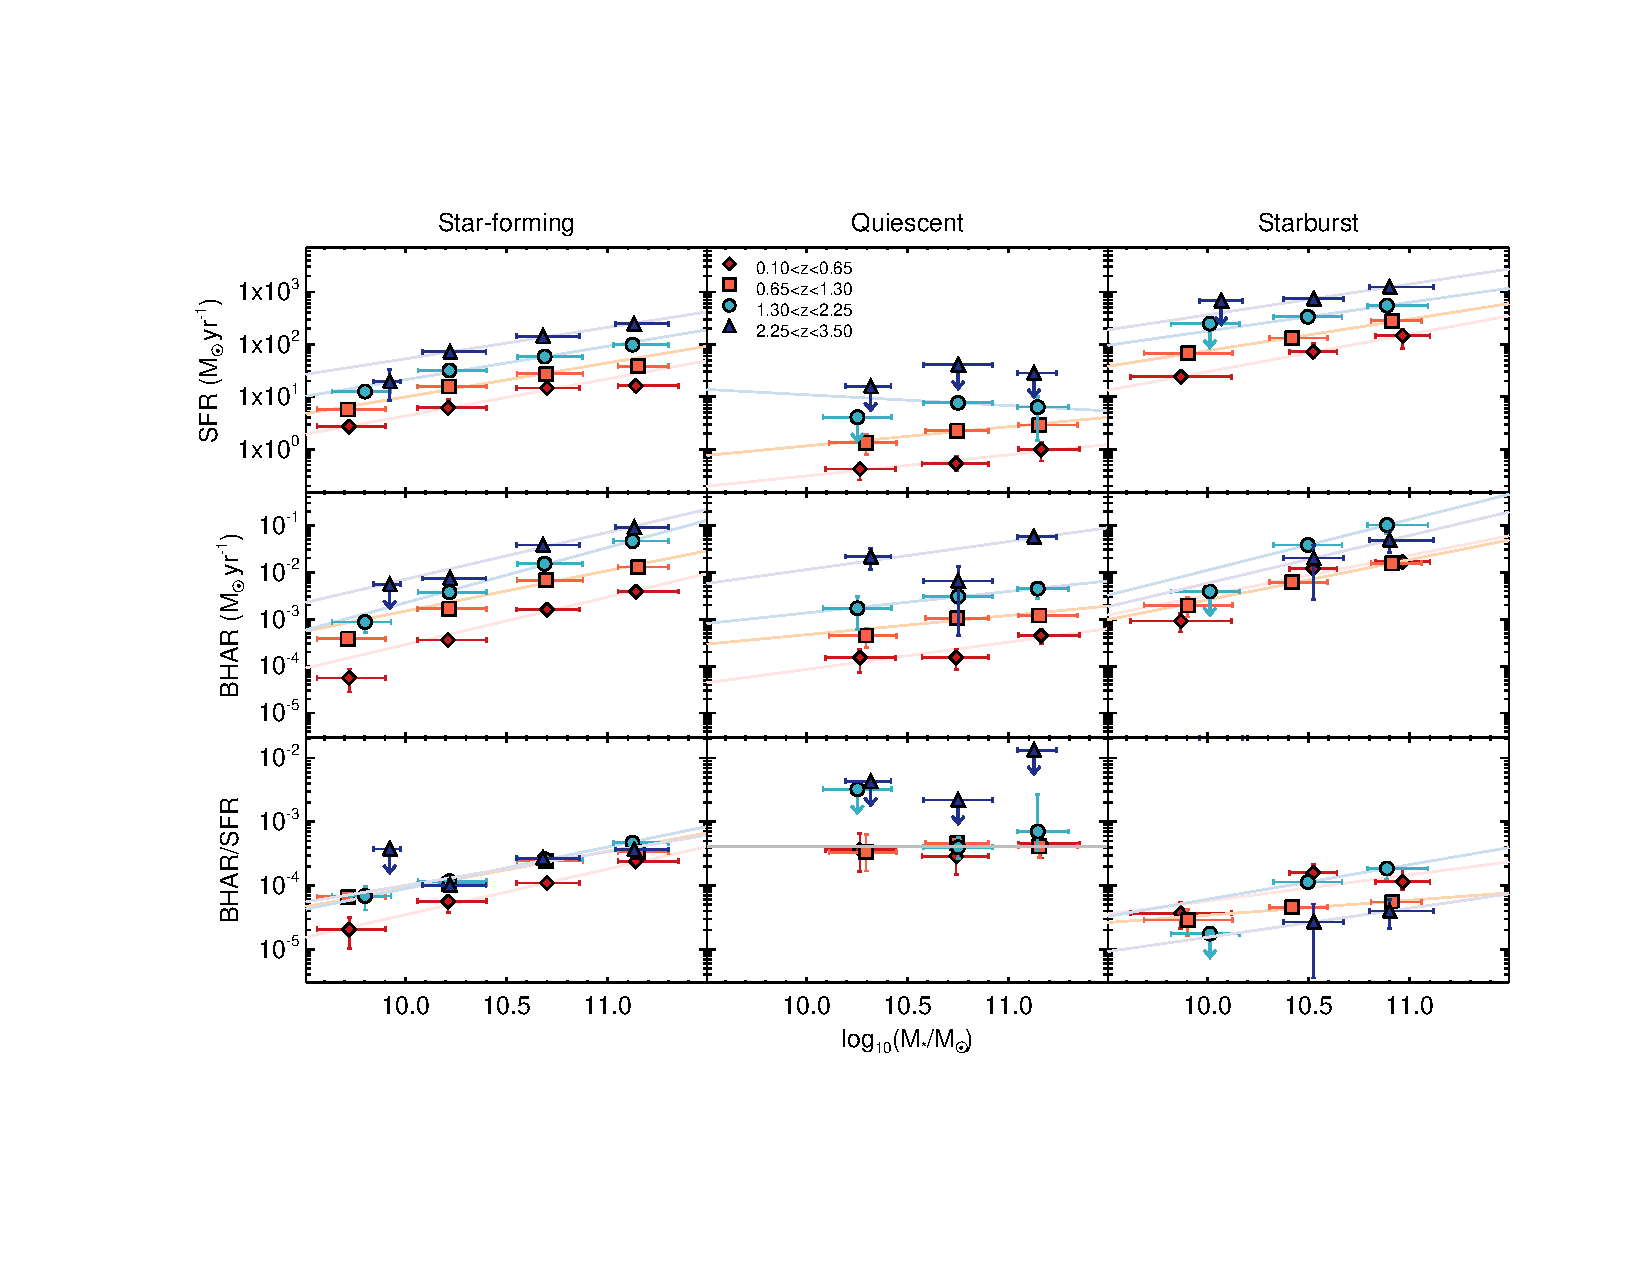
\includegraphics[trim={3.2cm 3.7cm 2cm 3.6cm}, clip,width=\textwidth]{Figs/SF_BH_all.pdf}
      \caption{Comparison between the average SFR and the average BHAR for the three samples: normal star-forming galaxies (left), quiescent galaxies (center), and starburst galaxies (right).
      In all plots data points are color- and shape-coded according to the redshift interval. The data points are the median value, and vertical errors represent the 5th and 95th percentile. We show an upper limit (the 95th percentile) for the data points whose SFR or BHAR 5th percentile is compatible with zero and for starburst galaxies at high redshift and low mass, where our sample is inclomplete in mass.
      The error bars shown on the stellar masses correspond to $1~\sigma$ of the distribution. The solid light colored lines are the best fits and are color-coded according to each redshift bin (see Table~\ref{table:all_fitpar}). 
      Top panel: M$_*$-SFR relation. 
      Middle panel: M$_*$-BHAR relation.
      Bottom panel: BHAR-to-SFR ratio as a function of stellar mass. The dotted gray line for quiescent galaxies is at a constant value of BHAR/SFR$=3.8\times 10^{-4}$.
              }
         \label{fig:SF_BH_all}
   \end{figure*}
%-------------------------------------------------------------
%                                             Simple A&A Table
%-------------------------------------------------------------
% restore,'all_var_pt2.sav'
% print,fit_par_sfr[0,*,*], format='(f20.2)'
% print,sigma_sf[0,*,*], format='(f20.2)'
% print,fit_par_bhar[0,*,*], format='(f20.2)'
% print,sigma_bh[0,*,*], format='(f20.2)'
% print,fit_par_ratio[0,*,*], format='(f20.2)'
% print,sigma_sfbh[0,*,*], format='(f20.2)'
% print,fit_par_ratio[1,0,0], format='(f20.2)'
% print,fit_par_ratio[1,0,1], format='(f20.2)'
\begin{table*}
\caption{Fit parameters of the relations in Fig.~\ref{fig:SF_BH_all}. The equations we used are for $\log_{10}{\rm SFR}=m\,\log_{10}{\rm M}_*+q$; for $\log_{10}{\rm BHAR}=m\,\log_{10}{\rm M}_*+q$; and for the ratio $\log\frac{\text{BHAR}}{\text{SFR}}=\alpha\,\log\text{M}_*+\beta$.}             % title of Table
\label{table:all_fitpar}      % is used to refer this table in the text
\centering                          % used for centering table
\begin{tabular}{l | c c | c c | c c }        % centered columns % >{\boldmath} for bold columns using math
\hline\hline                 % inserts double horizontal lines
              & SFR                 &                  & BHAR              &                   & BHAR/SFR          &                    \\
Redshift bin  & $m $                & $q$              & $m$               & $q$               & $\alpha$          & $\beta$            \\    % table heading \textbf{Star forming} &             &                  &                   &                   &                   &                    \\
\hline                                                                                                           
\textbf{Star-forming} &              &                  &                   &                   &                   &       \\
$0.10<z<0.65$ & $ 0.71  \pm 0.02  $ & $ -6.4 \pm 0.2 $ & $ 1.02 \pm 0.03 $ & $-13.7 \pm 0.3$ & $ 0.72 \pm 0.09 $ & $ -11.6  \pm 0.9  $ \\    
$0.65<z<1.30$ & $ 0.649 \pm 0.013 $ & $ -5.49\pm 0.13$ & $ 0.87 \pm 0.02 $ & $-11.5 \pm 0.2$ & $ 0.58 \pm 0.03 $ & $  -9.9  \pm 0.4  $ \\
$1.30<z<2.25$ & $ 0.639 \pm 0.018 $ & $ -5.06\pm 0.19$ & $ 1.18 \pm 0.03 $ & $-14.4 \pm 0.3$ & $ 0.65 \pm 0.04 $ & $ -10.6  \pm 0.4  $ \\
$2.25<z<3.50$ & $ 0.60  \pm 0.04  $ & $ -4.3 \pm 0.4 $ & $ 1.00 \pm 0.05 $ & $-12.2 \pm 0.5$ & $ 0.53 \pm 0.07 $ & $  -9.3  \pm 0.7  $ \\
\hline
\textbf{Quiescent}  &               &                &                   &                   &                   &                     \\
$0.10<z<0.65$     & $ 0.40\pm 0.14$ & $-4.5 \pm 1.5$ & $ 0.58\pm 0.17$ & $ -9.9 \pm 1.9 $  &                   &                     \\    
$0.65<z<1.30$     & $ 0.37\pm 0.15$ & $-3.6 \pm 1.6$ & $ 0.41\pm 0.16$ & $ -7.4 \pm 1.7 $  &   -               & $ -3.38 \pm 0.07 $  \\
$1.30<z<2.25$     & $-0.2 \pm 0.5 $ & $ 3.1 \pm 4.9$ & $ 0.5 \pm 0.2 $ & $ -7.6 \pm 2.4 $  &                   &                     \\
$2.25<z<3.50$     & -               & -              & $ 0.59\pm 0.18$ & $ -7.9 \pm 2.0 $  &                   &                     \\
\hline
\textbf{Starburst}  &              &                  &                   &                   &                   &                    \\
$0.10<z<0.65$ & $ 0.73 \pm 0.05 $  & $ -5.8 \pm 0.5 $ & $ 0.86 \pm 0.09 $ & $ -11.0 \pm 1.0 $ & $ 0.36 \pm 0.12 $ & $ -7.9 \pm 1.3 $  \\  
$0.65<z<1.30$ & $ 0.61 \pm 0.03 $  & $ -4.3 \pm 0.3 $ & $ 0.86 \pm 0.10 $ & $ -11.1 \pm 1.1 $ & $ 0.22 \pm 0.11 $ & $ -6.7 \pm 1.2 $  \\
$1.30<z<2.25$ & $ 0.54 \pm 0.07 $  & $ -3.1 \pm 0.8 $ & $ 1.08 \pm 0.11 $ & $ -12.8 \pm 1.2 $ & $ 0.54 \pm 0.15 $ & $ -9.6 \pm 1.6 $  \\
$2.25<z<3.50$ & $ 0.59 \pm 0.14 $  & $ -3.4 \pm 1.5 $ & $ 1.0  \pm 0.7  $ & $ -12.5 \pm 7.3 $ & $ 0.44 \pm 0.72 $ & $ -9.2 \pm 7.8 $  \\
\hline                                   %in$serts single line
\end{tabular}
\end{table*}
%----------------------------------------------------------------- 

%REFERENCES TO FIG 3.
\section{Constraining the coevolution of galaxy and black hole accretion} \label{sec:BH_SF}
In Figure~\ref{fig:SF_BH_all} we compare the SFR and the BHAR as a function of M$_*$ for the three categories of galaxies.
In the left column we show star-forming galaxies, in the middle column we list quiescent galaxies, and the right column contains starburst galaxies. 
The top panel shows the total SFR$_{\rm UV+IR}$ (SFR$_{\rm IR}$ only for starburst galaxies, see Sec.~\ref{ssec:SFR}) for all the redshift bins, the middle panel shows the BHAR of the sample obtained from the X-ray luminosity (Figure~\ref{fig:L_X}) using Equation \ref{eq:BHAR}, and the bottom panel presents the ratio between BHAR and SFR. 
We show linear fits in all panels except for the BHAR/SFR of quiescent galaxies where we report the average value of all redshifts and mass bins because no evolutionary trends are apparently visible.
The best-fit parameters are shown in Table \ref{table:all_fitpar}.

\subsection{Star-forming galaxies}
        For star-forming galaxies, the top panel shows the well-known evolution of the main-sequence of star-forming galaxies with time: the SFR follows a sublinear relation (in logaritmic units) with stellar mass that evolves in normalization with redshift, maintaining an almost constant slope and a bend at high M$_*$ in the two lower redshift bins. This bend was introduced by including the quiescent $24\mu m$ MIPS/\textit{Spitzer} detected sources, which as described above, are concentrated at high masses and lower redshifts. The median SFR$_{\rm UV}$ of the sample is  lower than the median SFR$_{\rm IR}$ by a factor that varies from 3 (low mass) to 100 (high mass, see Table~\ref{tab:SF_prop}), which means that the SFR$_{\rm UV}$ is negligible in most cases.

The observed BHAR distribution has a higher slope in the log-log plane; it is slightly superlinear 
(a direct consequence of the L$_\text{X}$-M$_*$ relation). 
    It is present at all considered redshifts and evolves with it.
    We note that the decrease in BHAR normalization evolves faster in the lowest redshift bin, but maintains a more constant increase at earlier cosmic epochs. The total decrease in BHAR at given M$_*$ is about 1.5~dex, and in SFR, the decrease is about 1-1.2~dex.


The ratio of BHAR to SFR provides interesting insights into how these two phenomena relate to each other. It increases with mass with a slope that varies in the $\sim0.5-0.7$ range, decreases at higher redshifts, and does not evolve in normalization. 
The positive slope of the BHAR/SFR can be interpreted as 
an indication of
an increased accretion efficiency in galaxies with high stellar mass by driving the infalling gas directly toward their inner core, which fuels a faster accretion onto the black hole. This can also be considered to mean that the main driver of the black hole accretion is not time, but the initial stellar mass. 
We note that the analogy between the increase in the BHAR/SFR as a function of stellar mass and the increase in the density of the central kiloparsec of the galaxy $\Sigma_1$ with mass \citep{2013ApJ...776...63F,2017ApJ...840...47B}. It has been proposed that more massive galaxies might have denser cores that might allow for a faster growth of the black hole.


\subsection{Quiescent galaxies}
In the central column of Fig.~\ref{fig:SF_BH_all} we show the data points of the quiescent galaxies. As expected, the SFR of these galaxies is lower than that of star-forming galaxies.
The two lower redshifts show a weak dependence of stellar mass, with a slope of $\sim0.4$, 
and the evolution with redshift in the bins in which we were able to constrain the SFR is also clear.
The reason might be that high-redshift elliptical galaxies are of a different nature than local galaxies and have higher percentages of gas \citep{2018NatAs...2..239G}, but part of the emission might also originate in dust cirrus illuminated by older stellar populations \citep{2007ApJ...657..810D, 2015A&A...573A.113B}. 
Another factor that may be contributing to the evolution we see is a small fraction of misclassified star-forming galaxies at high redshift. This may be caused by galaxies that emit in the MIPS band but lie below the detection threshold or by cross-contamination in the NUV$ - r / r - J$ because the uncertainty in the estimation of the rest-frame magnitudes that are required to classify a galaxy in the color-color diagram is higher. Overall, it is not possible to determine whether this evolution in time and mass dependence of quiescent galaxies and their mass dependence is significant, especially because we are able to constrain only these high-mass bins.

 For comparison with star-forming galaxies, we note that the median SFR$_{\rm UV}$ of the quiescent sample is lower by a factor of about 15 than the median SFR$_{\rm IR}$ $ \text{}$ (see Table~\ref{tab:Q_prop}). This means that the SFR$_{\rm UV}$ is negligible in most cases.

We are better able to constrain the BHAR at all redshifts and see a redshift evolution and weak dependence on stellar mass,with a slope $\sim0.5,$ even though it is difficult to analyze the slope evolution because of the small number of data points.
The normalization in BHAR is higher than in SFR, that is, the normalization of the BHAR is similar to the normalization of BHAR in star-forming galaxies, while the SFR of quiescents is clearly lower than that of star-forming galaxies. This indicates that the efficiency in accreting material onto the black hole is higher than in forming stars in galaxies at this late stage in the life of galaxies: the gas present in the galaxy ``prefers'' to fall into the black hole rather than form stars. This is consistent with the results of \citet{2018NatAs...2..239G}, who reported that a substantial amount of gas is available at high redshift in quiescent galaxies. This is then probably consumed less efficiently than in star-forming galaxies.
    
    The BHAR/SFR of quiescent galaxies, for the few mass and redshift bins where it was possible to constrain this, shows a flat trend in mass that is compatible with a constant value of $4.2\times10^{-4}$ at all redshifts and M$_*$. This value, obtained as a weighted mean of the data points, is a confirmation of the trends we have seen for BHAR and SFR: it is compatible with the values obtained for the highest mass bin of star-forming galaxies, 
    indicating that even though the ability of a galaxy to form stars has decreased in these galaxies, the efficiency of attracting the gas to the black hole did not.


\subsection{Starburst galaxies}
In the right column of Figure~\ref{fig:SF_BH_all} we show the starburst sample. By selection, FIR-selected starbursts have higher SFR than normal star-forming galaxies; the evolution in time is clear, as is the dependence on M$_*$.  

In starburst galaxies, the BHAR shows a close to linear dependence on mass and a weak evolution in redshift: values range in about $\text{}1$~dex, but the highest redshift bin has a lower normalization than the previous one, differently from what is seen in the other phases of galaxy life. 
This decrease in BHAR, which is not as pronounced as the decrease in star-forming galaxies (about $\sim1.5$~dex) causes them to slowly become starburst galaxies (i.e., higher than main-sequence galaxies) in the black hole accretion as well at lower redshift. 
    
    There is no clear evolution in the normalization of the BHAR/SFR, but it is interesting to note that the highest redshift bin shows the lowest normalization, which indicates that in these extremely star-forming galaxies black hole accretion was disfavored at higher redshifts. The slope appears to be positive and of about $0.2-0.4$.
    
    We tested selecting a starburst galaxy sample using the main-sequence from \citet{2011ApJ...739L..40R} with a redshift evolution as in \citet{2012ApJ...747L..31S}, SFR$_{\rm MS}(z)\propto (1+z)^{2.8}$. This selection assumed no bend on the main-sequence at high stellar masses and was calibrated up to $z\sim 2$. When we extrapolated this evolution to higher redshifts, we found a higher normalization than was reported by \citet{2015A&A...575A..74S}, which instead was calibrated up to $z\sim5$. This starburst selection led to no significant differences in the SFR of the sample, but to slightly lower BHAR values. We were also unable to constrain the X-ray luminosities of starbursts in the highest redshift bin. This suggests that the most starbursty galaxies accrete their black hole even less. This finally resulted in a flatter trend of the BHAR/SFR against stellar mass.


%%%% end FIGURE 3
\subsection{Comparisons with the literature} \label{sec:compare}
In Figure~\ref{fig:conf_yang} we compare our results for the star-forming sample with results from the literature. We show our data points from 
Figure~\ref{fig:SF_BH_all} in the left column and compare them with results from \citet{2018MNRAS.475.1887Y} as solid lines, with results from \citet{2019MNRAS.484.4360A} as a dashed beige line, and with results from \citet{2019ApJ...885L..36D} as a dot-dashed violet line.

         Our data points qualitatively agree with those from \citet{2018MNRAS.475.1887Y} in the three panels% of Figure~\ref{fig:conf_yang}
         . \citet{2018MNRAS.475.1887Y} selected their star-forming sample from GOODS-N, GOODS-S, and COSMOS UltraVISTA DR1 based on the SFR from SED fitting with a SFR threshold at $1.3$~dex below the main-sequence. SFRs are from \citet{2015ApJ...801...97S} and \citet{2019ApJS..243...22B}). Their average SFRs are slightly higher than ours. They also reported that the BHAR of the lowest redshift bin is separated more than the BHAR between the other bins.
         
The BHAR/SFR of \citet{2019MNRAS.484.4360A} has a linear trend with mass with a higher slope than ours. Their BHARs were obtained with the same method as in \citet{2018MNRAS.474.1225A}. Their SFRs are from SED fitting from the UV to MIR, which means that the FIR was not included. Together with the constant bolometric correction they used, this might lead to the higher slope value.
   
   We also compared our data points with the relation found by \citet{2019ApJ...885L..36D} through an empirically motivated model that successfully reproduces the observed X-ray luminosity function (XLF) since $z\sim3$. With this model, they found a growth in two steps: until the galaxy reaches a critical mass, the black hole growth lags behind it, and then, as the stellar mass increases, the BHAR is enhanced with respect to the SFR, following a superlinear relation very similar to ours, except for an offset of $\sim0.1-0.3$~dex.

%-------------------------------------------------------------
%                                    One column rotated figure
%-------------------------------------------------------------
   \begin{figure}%[H]
   \centering
   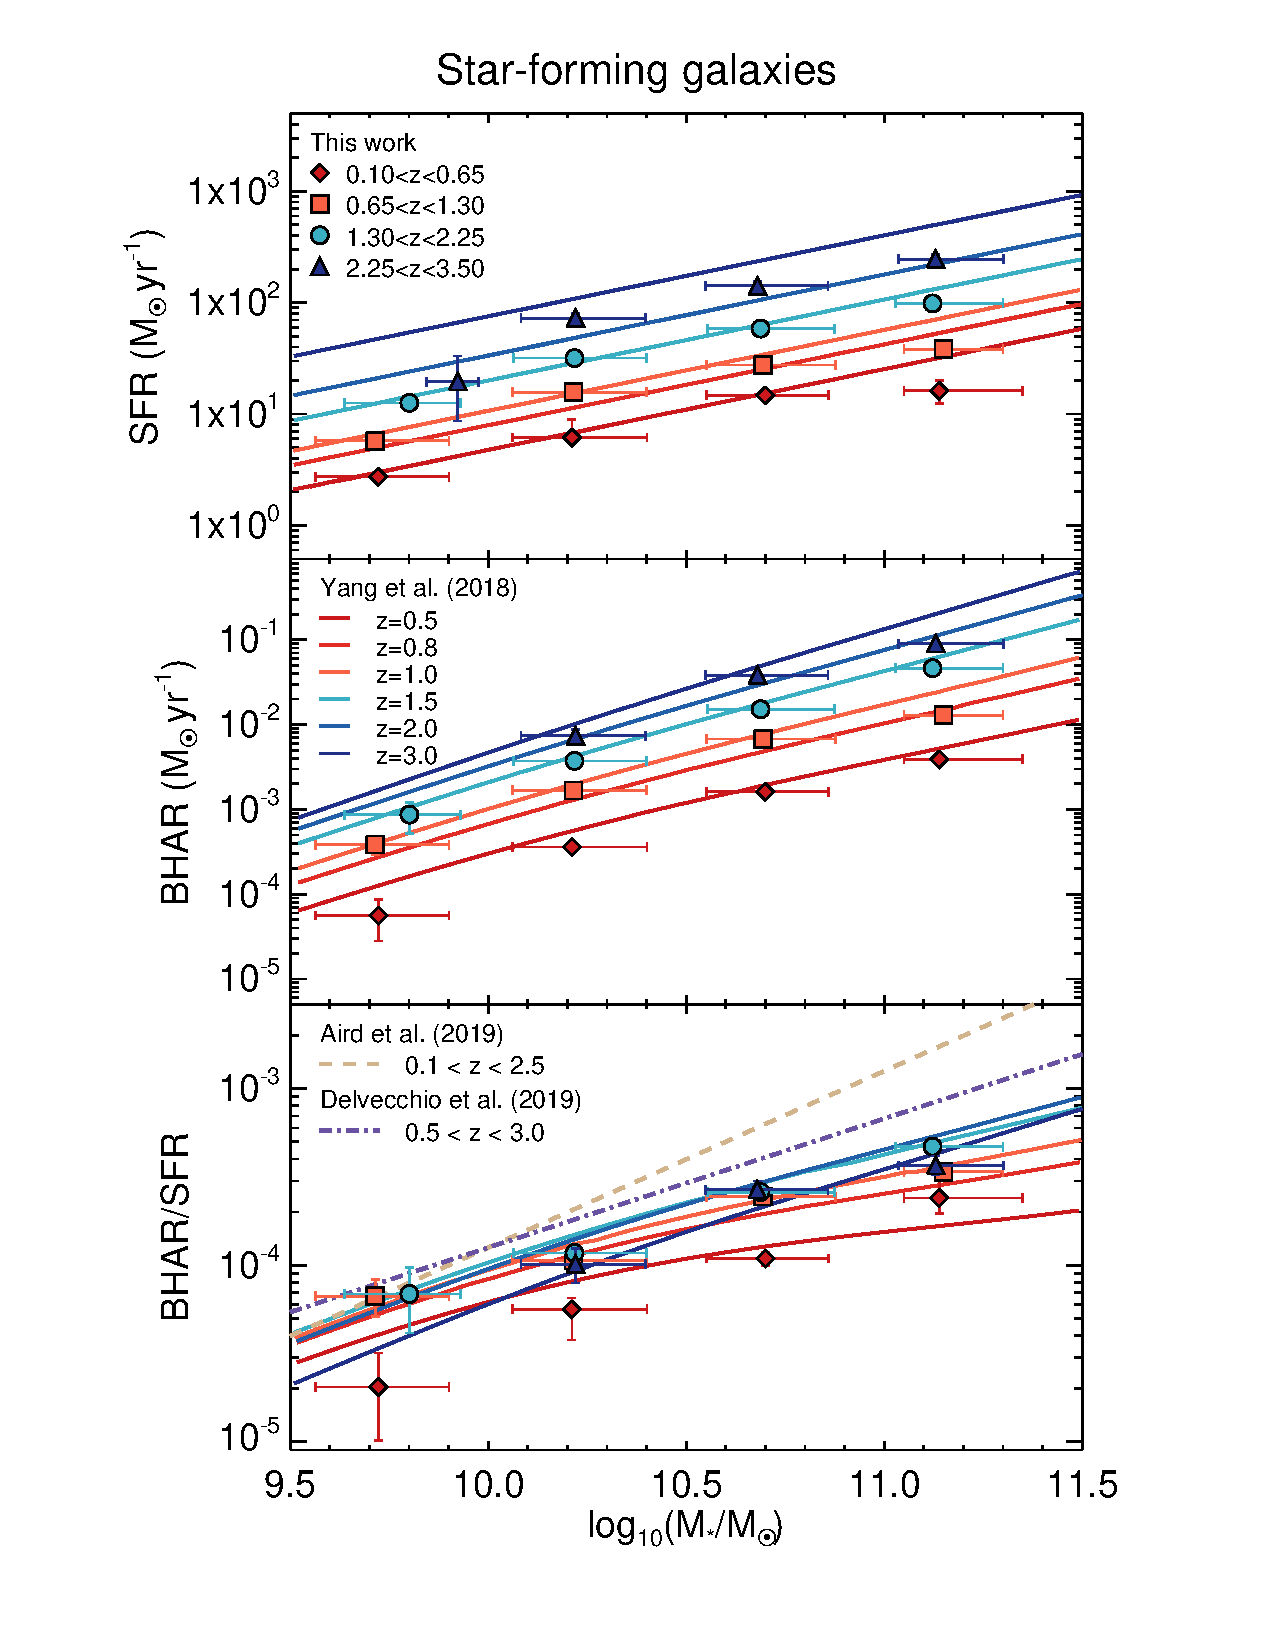
\includegraphics[trim={1.8cm 1.5cm 2.3cm 0.8cm}, clip, width=0.7\textwidth]{Figs/SF_BH_SF_Yang.pdf}
      \caption{ Comparison between our results for star-forming galaxies and data from \citet{2018MNRAS.475.1887Y}, \citet{2019MNRAS.484.4360A}, and \citet{2019ApJ...885L..36D}.
            Data points are taken from the left column of Figure~\ref{fig:SF_BH_all}, and the curves are adapted from Figure~14 in \citet{2018MNRAS.475.1887Y} and were scaled to the same $k$-correction as we adopted here.
            Data from \citet{2019MNRAS.484.4360A} are taken from Fig.~13.
              }
         \label{fig:conf_yang}
   \end{figure}
%--------------------------------------------------------------------

%REFERENCES TO FIG 4.
\section{Comparison between the evolution of sBHAR and sSFR} \label{sec:specifics}
%
%\subsection{sSFR and sBHAR} \label{ssec:sSFR}
We computed the average sSFR (i.e., specific SFR, SFR/M$_*$) and the sBHAR (i.e., specific BHAR, BHAR/M$_\text{BH}$) for all the bins in M$_*$ and $z$. In this section we describe how the sBHAR was derived and we discuss the results.
%----------------------------------------------------------------- 

   \begin{figure*}
   \centering
   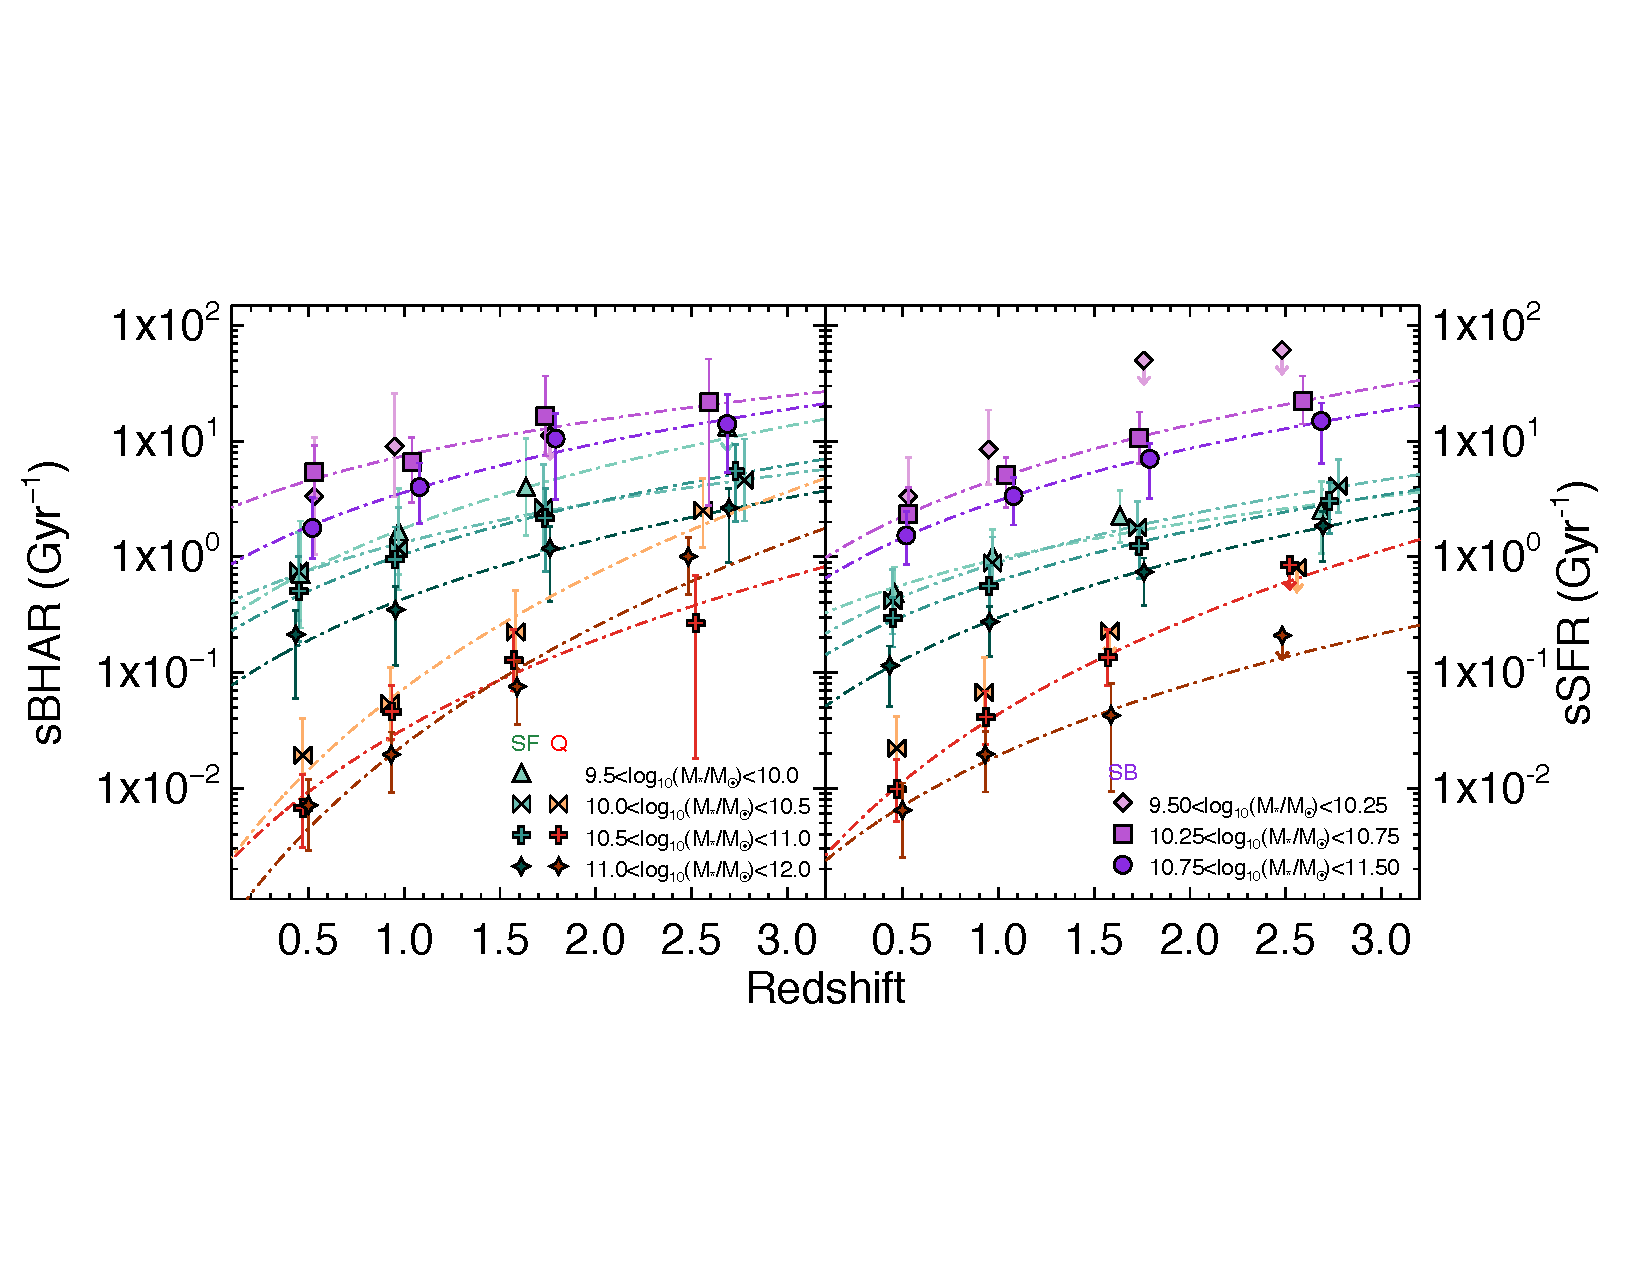
\includegraphics[trim={0 4cm 0.5cm 5.1cm}, clip,width=\textwidth]{Figs/sBHAR_all.pdf}
      \caption{ Specific black hole accretion rate (left panel) and sSFR (right panel) as a function of redshift for star-forming (SF, in green), quiescent (Q, in red), and starburst (SB, in purple) galaxies. The data points are placed at the median redshift of each mass bin and are coded in shape and color according to their median mass and type. Error bars represent the 90\% confidence interval associated with each measure. We show an upper limit (the 95th percentile) for the data points whose sBHAR/sSFR 5th percentile is compatible with zero and for starburst galaxies at high redshift and low mass, where our sample is incomplete. The dot-dashed line is the best fit of the data to the curve $sBHAR(sSFR)=\delta\, (1+z)^{\gamma}$ and is color-coded according to the galaxy type and mass bin.
              }
         \label{fig:sBHAR_all}
   \end{figure*}
%-----------------------------------------------------------------
%
\subsection{Black hole mass estimate}
In order to estimate the black hole mass M$_{\text{BH}}$ , we considered the fits in the bottom panels of Fig. \ref{fig:SF_BH_all} and in the right column of Table~\ref{table:all_fitpar}, obtained from the equation
\begin{equation}  \label{eq:ratio_fit}
\centering
\log\frac{\text{BHAR}}{\text{SFR}}=\alpha\log\text{M}_*+\beta.
\end{equation}

The general equation we used for the computation is
\begin{equation}  \label{eq:ratio_comp}
\centering
\log\frac{\text{BHAR}}{\text{SFR}}=
\log\frac{\dot{\text{M}}_{\text{BH}}}{\dot{\text{M}}_*}=
\log\frac{\partial\text{M}_{\text{BH}}}{\partial\text{M}_*}= 
\alpha \log\text{M}_* + \beta,
\end{equation}
which is valid only under the assumption that the growth rates of stellar and black hole mass are constant in time. The ratios we measure show almost no evolution up to $z\sim3.5,$  which appears to justify this assumption.
%Therefore our values, especially at lower redshift, are to be considered upper limits of the evolution, given that they are obtained assuming growths at the lowest rates observed. 
By integrating Equation~\ref{eq:ratio_comp} with respect to stellar mass, we obtained the estimate of the M$_\text{BH}$ of each stellar mass and redshift bin:
\begin{equation}  \label{eq:M_bh}
\centering
\text{M}_\text{BH}=\frac{10^\beta}{1+\alpha}\,\text{M}_*^{1+\alpha},
\end{equation}
where $\alpha$ and $\beta$ are the same parameters in Table~\ref{table:all_fitpar} and are the parameters we used in the computation. It follows from Eq.~\ref{eq:M_bh}  that the black hole mass has a superlinear dependence on stellar mass in star-forming and starburst galaxies, but M$_{\rm BH}$ has a linear dependence on M$_*$ in quiescent galaxies.

If instead of performing an indefinite integral we integrate between the initial masses ($\text{M}_{*,i}$ and $\text{M}_{\text{BH},i}$) and the final (observed) masses, the integrated Equation~\ref{eq:ratio_comp} would read
\begin{equation}  \label{eq:M_bh_compl}
\centering
\text{M}_\text{BH}=\frac{10^\beta}{1+\alpha}\,(\text{M}_*^{1+\alpha}-\text{M}_{*,i}^{1+\alpha})+\text{M}_{\text{BH},i}
.\end{equation}
We assumed that the initial black hole mass is lower by at least an order of magnitude ($\lesssim10^5\text{M}_*$) than the final mass, however, therefore it is negligible. The initial stellar mass instead eludes us, and becuase we subtracted it, our $\text{M}_\text{BH}$ is an upper limit. We therefore decided not to use the complete expression of $\text{M}_\text{BH}$ in Eq.~\ref{eq:M_bh_compl}, but the expression in Eq.~\ref{eq:M_bh}.

\subsection{Results for the specific accretions}
Figure~\ref{fig:sBHAR_all} shows the redshift evolution of the sBHAR (estimated using $\text{M}_{\text{BH}}$ from Eq.~\ref{eq:M_bh}) and sSFR for star-forming, quiescent, and starburst galaxies.
sBHAR and sSFR have a decreasing trend toward lower redshift for the three galaxy types, and the stellar mass shows a split: low-mass galaxies have higher values than high-mass galaxies, although this split is often not significant within the error bars.

        These trends confirm what has been reported before about these specific accretions. They also  provide new interesting insight.
        The spread in stellar mass is consistent with downsizing: it implies that high-mass galaxies have accreted most of their M$_*$ and M$_\text{BH}$ at high redshift and their accretion decreased fast and steeply, whereas low-mass galaxies have accreted their mass more slowly, but   their accretion rate decreased more slowly with  time. Downsizing has previously been observed for stellar mass \citep{1996AJ....112..839C, 2006A&A...453L..29C} and black hole luminosity (e.g., \citealt{2004MNRAS.351..169M} but also \citealt{2004MNRAS.354.1020S, 2009ApJ...690...20S, 2015ApJ...810...74A}, who reached similar conclusions from continuity equation arguments). 
        In our plots, downsizing can be observed in the steepening of the slope $\gamma$ at higher masses in star-forming and starburst galaxies and in the two specific accretions, which indicate a faster decrease for higher masses. Downsizing can also be seen in
        high-mass galaxies (darker data points), which show lower sSFR(sBHAR) on average than lower mass galaxies. This means that at even at higher redshifts, the most massive galaxies have already accreted most of their stellar and black hole mass, even though within the error bars, sSFR (sBHAR) data points are often compatible with a unique value for all stellar masses at a given redshift. In particular, this trend would not be present in star-forming galaxies without introducing the dependence of the black hole mass on the slope $\alpha$ from Equation~\ref{eq:ratio_fit}.
        %What is interesting is that galaxies in all different phases of their evolution show signs of downsizing, meaning that the different phases of evolution don't even out this growing mode.
%       It is interesting to note that galaxies show signs of downsizing in all phases of their evolution.

We show in Figure~\ref{fig:sBHAR_all} the best fits to the data when a redshift evolution of the form
sBHAR~(sSFR)$=\delta\, (1-z)^{\gamma}$ is adopted, which we applied to each mass bin for all galaxy types when at least three data points were available\footnote{Fits performed with IDL/MPFIT \citep{2009ASPC..411..251M}}. 
The sSFR and sBHAR for star-forming and starburst galaxies are compatible with $\gamma=2.8,$ as in \citet{2012ApJ...747L..31S}, within $1\sigma$, but this is not the case for quiescent galaxies, which have higher slopes with a steeper decreases in specific accretions in time. Interestingly, we do not note a significant exponent difference between sBHAR and sSFR at given galaxy type.
When we consider that there may be a small contribution from misclassified star-forming galaxies in the quiescent sample, especially at high redshift, the real trend may be even flatter, and approach a slope $\gamma=2.8$.
We do see a difference in the normalizations of the relations, which show lower specific accretions for quiescent galaxies, followed by star-forming galaxies, and finally, starburst galaxies, which tend to have higher specific accretions.
When  the normalizations for the two specific accretions are compared, they are very similar in the case of starburst galaxies, while star-forming galaxies have a higher normalization for the sBHAR and quiescent galaxies show higher sBHAR than sSFR at high $z$.

    Because the inverse of sSFR and sBHAR can be considered as the mass-doubling timescale of the M$_*$ and of the SMBH, this means that the stellar mass of the galaxy and the SMBH are accreted faster in starburst and star-forming galaxies, which especially at high redshift are still efficient and can quickly double their mass. Quiescent galaxies are instead slower and have mass-doubling timescales of about a Hubble time or more. The black hole mass-doubling time of star-forming galaxies instead seems to be shorter than the stellar mass black hole mass-doubling time at every redshift and mass bin.
    
These similar evolution trends between sBHAR and sSFR strongly suggest a connection between the two accretions that appears to be present in all galaxy life phases. Star-forming galaxies appear to dominate the accretion histories; they are the most numerous galaxies and are able to substantially accrete their stellar and black hole masses. Starburst galaxies, with a higher capability of accretion but short-lived episodes, and quiescent galaxies, although their accretion capabilities are lower, appear to be able to accrete their black hole more efficiently than their stellar mass.
   
%-------------------------------------------------------------
%                                             Simple A&A Table
%-------------------------------------------------------------
% restore,'specific_fits_par.sav'
% print, sbhar_fit_gen[0,3:*,*], format='(f20.2)'
% print, sbhar_gen_sigma[0,3:*,*], format='(f20.2)'
% print, sbhar_fit_gen[1,4:*,*], format='(f20.2)'
% print, sbhar_gen_sigma[1,4:*,*], format='(f20.2)'
% print, sbhar_fit_gen[2,1:*,*], format='(f20.1)'
% print, sbhar_gen_sigma[2,1:*,*], format='(f20.1)'
% print, ssfr_fit_gen[0,3:*,*], format='(f20.2)'
% print, ssfr_gen_sigma[0,3:*,*] , format='(f20.2)'
\begin{table*}
\caption{Fit parameters of the relations in Fig.~\ref{fig:sBHAR_all}. The equation we used is sBHAR~(sSFR)$=\delta\, (1 +z)^{\gamma}$.}             % title of Table
\label{table:specific_fitpar}      % is used to refer this table in the text
\centering                          % used for centering table
\begin{tabular}{l | c c | c c }        % centered columns % >{\boldmath} bold columns
\hline\hline                 % inserts double horizontal lines
Mass bins                   & sBHAR parameters      &                 & sSFR parameters     &                 \\
$\log_{10}($M$_*$/M$_\sun)$ & $\delta$              &  $\gamma$       & $\delta$            &  $\gamma$       \\
\hline                                                                                                  
\textbf{Star-forming}       &                       &                 &                     &                 \\
 9.5--10.0                  & $ 0.2  \pm 0.3  $     & $ 2.9 \pm 1.8 $ & $ 0.28 \pm 0.13 $   & $ 1.8 \pm 0.5 $ \\
10.0--10.5                  & $ 0.3  \pm 0.3  $     & $ 2.0 \pm 0.9 $ & $ 0.17 \pm 0.09 $   & $ 2.4 \pm 0.6 $ \\
10.5--11.0                  & $ 0.18 \pm 0.14 $     & $ 2.6 \pm 0.8 $ & $ 0.11 \pm 0.05 $   & $ 2.5 \pm 0.5 $ \\
11.0--12.0                  & $ 0.06 \pm 0.04 $     & $ 2.9 \pm 0.7 $ & $ 0.039\pm 0.016$   & $ 2.9 \pm 0.4 $ \\
\hline
\textbf{Quiescent}          &                       &                 &                     &                 \\
10.0--10.5                  & $ 0.0015 \pm 0.0012 $ & $ 5.6 \pm 0.9 $ & -                   & -               \\
10.5--11.0                  & $ 0.0016 \pm 0.0009 $ & $ 4.4 \pm 0.7 $ & $0.0017 \pm 0.0012$ & $ 4.7 \pm 1.0 $ \\
11.0--12.0                  & $ 0.0004 \pm 0.0003 $ & $ 5.8 \pm 0.8 $ & $0.0017 \pm 0.0013$ & $ 3.5 \pm 1.1 $ \\
\hline                      
\textbf{Starburst}          &                       &                 &                     &                 \\
 9.50--10.25                & -                     & -               & -                   & -               \\
10.25--10.75                & $ 2.3   \pm 1.6 $     & $ 1.7 \pm 0.9 $ & $ 0.8  \pm 0.4 $    & $ 2.6 \pm 0.5 $ \\
10.75--11.50                & $ 0.7   \pm 0.4 $     & $ 2.4 \pm 0.6 $ & $ 0.5  \pm 0.2 $    & $ 2.6 \pm 0.5 $ \\
\hline
\end{tabular}
\end{table*}
   
%-------------------------------------------------------------
%                                    One column rotated figure
%-------------------------------------------------------------
   \begin{figure}
   \centering
   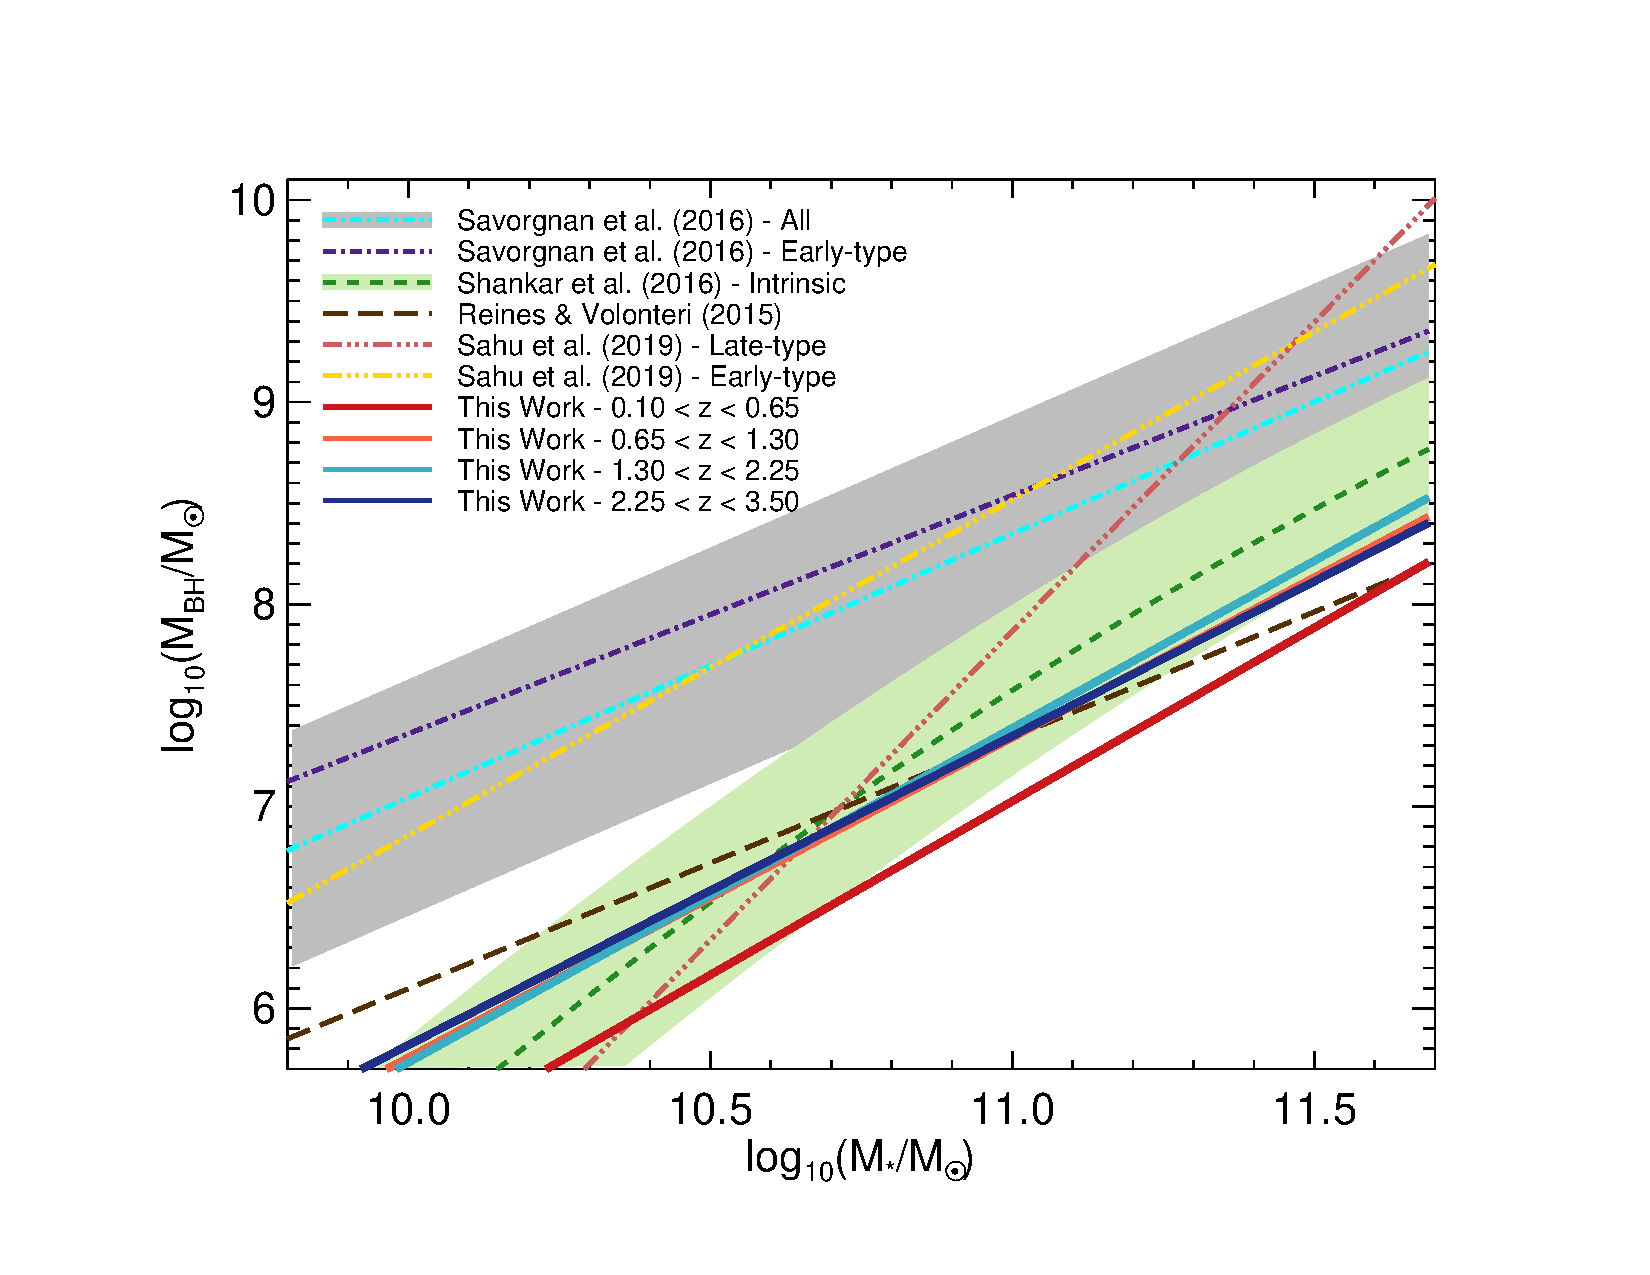
\includegraphics[trim={2cm 1.5cm 3cm 2cm}, clip, width=0.7\textwidth]{Figs/reFigureForSection7.pdf}
      \caption{ Comparison between our M$_*$ and M$_\text{BH}$ from Eq.~\ref{eq:M_bh} and parameters $\alpha$ and $\beta$ from Table~\ref{table:all_fitpar} for star-forming galaxies and results from models in the literature. Data from this work are shown as solid lines and are color-coded according to redshift as in Fig.~\ref{fig:SF_BH_all} and \ref{fig:conf_yang}.
      The relations from \citet{2016ApJS..222...10S} use the M$_*$ of the bulge.
      The gray shaded area is the confidence range for \citet{2016ApJS..222...10S}, and the light green are is the confidence range for \citet{2016MNRAS.460.3119S}.
              }
         \label{fig:comp_models}
   \end{figure}

%--------------------------------------------------------------------


\section{Relation between stellar mass and black hole mass} \label{sec:M_vs_M}
In Figure~\ref{fig:comp_models} we show our best-fit resulting M$_\text{BH}$-M$_*$ relations for star-forming galaxies derived from Eq.~\ref{eq:M_bh} with parameters from Table~\ref{table:all_fitpar}. These are superlinear relations with approximately M$_{\rm BH}\propto\text{M}_*^{1.6}$.
Our stellar masses are to be considered lower limits because as pointed out in \citet{2003ApJ...585L.117B}, stellar masses obtained using \citet{2003MNRAS.344.1000B} models lead to lower mass-to-light ratios and therefore to systematically lower stellar mass estimates at a given luminosity. A possible correction in our stellar masses that would cause them to agree better with those of \citet{2003ApJ...585L.117B} (increase of $\sim0.25$~dex) would further support our results.

We note that recent scaling relations proposed by other groups for both early-type galaxies and late-type galaxies show different scaling slopes and normalizations. \citet{2019ApJ...876..155S} find a relation for early-type galaxies that is similar in both slope and normalization to the lines of \citeauthor{2016ApJS..222...10S} (who used bulge stellar masses. See \citet{2016MNRAS.460.3119S, 2019MNRAS.485.1278S} for details) reported in Fig. \ref{fig:comp_models}. For late-type galaxies, \citet{2019ApJ...876..155S} find a lower normalization, more consistent with our relation around M$_*\sim 10^{10.5}{\rm M}_\odot$, but a much steeper slope of $\sim3.0\pm 0.5$, about $3\sigma$ steeper than ours. All in all our results point to either lower normalizations or flatter slopes than those identified from local dynamically measured SMBHs.
%Our relations are significantly below in normalization with respect to the M$_\text{BH}$-M$_*$ relations that characterize the secure total and early-type samples of local galaxies with dynamically measured SMBHs by \citeauthor{2016ApJS..222...10S} \citep[see][for details]{2016MNRAS.460.3119S, 2019MNRAS.485.1278S}. 
On the other hand, our resulting scaling relations have a similar normalization with those proposed by \citet{2015ApJ...813...82R} from local broad line AGN, despite them finding a close to linear relation, and agree well with 
%On the other hand, our resulting scaling relations agree well with those proposed by \citet{2015ApJ...813...82R} from local broad line AGN, and
the intrinsic scaling relation by \citet{2016MNRAS.460.3119S}. The latter have suggested that the local sample of (mainly) early-type galaxies with dynamically measured SMBH may be biased because a preselection might favor galaxies with the highest black hole masses and related gravitational radii. As recently suggested by \citet{2019MNRAS.485.1278S}, AGN samples that are clearly not affected by resolution-related selections effects should be closer to the intrinsic scaling relations. Our study further supports this view. 

We note that our normalization is inversely proportional to the radiative efficiency assumed in Eq.~\ref{eq:BHAR}. A match to the normalization of the local  M$_\text{BH}$-M$_*$ relation by \citeauthor{2016ApJS..222...10S} would require mean radiative efficiencies that are an order of magnitude lower. This is disfavored on other grounds \citep{2020MNRAS.493.1500S}. 

Our analysis adds key evidence, using IR data, to an increasing body of work \citep{2019ApJ...885L..36D,  2020ApJ...888...37D, 2020MNRAS.493.1500S, 2020ApJ...889...32S} on the weak evolution in the BHAR/SFR and its relatively low normalization relative to local raw dynamical M$_\text{BH}$-M$_*$ relations.%\LEt{again, please add at least one more sentence to form a paragraph}.

\section{Conclusions} \label{sec:conclusions}
We performed a statistical study on the COSMOS field in order to constrain the history and coevolution of star formation and black hole accretion in star-forming, quiescent, and starburst galaxies. We selected a mass-complete sample from the COSMOS 2015 catalog \citep{2016ApJS..224...24L} by classifying normal star-forming and quiescent galaxies through the NUV$ - r / r - J$ color-color diagram, and we selected starburst galaxies from the \textit{Herschel}-selected sample in \citet{2013MNRAS.432...23G}. We performed an X-ray stacking analysis and combined it with detected sources from \citet{2016ApJ...819...62C} in order to estimate the average X-ray luminosity and therefore average BHAR. We estimated the SFR from FIR stacking and UV SED fitting. Our main results are listed below.

   \begin{enumerate}
      \item We find a robust L$_{\rm X} - {\rm M}_*$ relation for star-forming galaxies at all considered redshifts. This relation evolves with an increasing normalization at higher redshifts. The X-ray luminosity of quiescent galaxies is close to that of star-forming galaxies, especially at low masses. At high masses, L$_\text{X}$ in quiescent galaxies is lower than in star-forming galaxies. The X-ray luminosities of starburst galaxies are compatible with star-forming at high redshifts and evolve mildly down to low redshift, where they are clearly higher than those of star-forming galaxies.
      \item The L$_{\rm X} - {\rm M}_*$ relation translates into a BHAR-M$_*$ relation in Fig.~\ref{fig:SF_BH_all} (middle row) that shows that the evolution of the BHAR in star-forming galaxies is faster at lower redshifts, it has a pronounced redshift evolution, and a weak mass dependence in quiescent galaxies. In turn, starburst galaxies have a marked mass dependence and a distinctive redshift evolution: going back in time, it reaches a maximum at $z\sim 1.7$ to then decrease again.
      \item BHAR in star-forming galaxies increases more with stellar mass than the SFR. In quiescent galaxies, the BHAR values lie close to the BHAR of star-forming galaxies, while the SFR of quiescent galaxies is clearly below the main-sequence. It is interesting that while the SFR of starburst galaxies continues to increase at higher redshifts, at the highest redshift in our study, the BHAR of these galaxies decreases.
      \item The ratio between BHAR and SFR in star-forming and starburst galaxies has a positive relation M$_*$ that is almost time-independent. The ratio is higher for quiescent galaxies, compatible with a flat trend in M$_*$ , indicating indicating a stronger tendency for this type of galaxy to accrete onto the black hole than to form stars, regardless of stellar mass. From this it follows that M$_{\rm BH}$ has a superlinear dependence on M$_*$ in star-forming and starburst galaxies, and the dependence is linear in quiescent galaxies.% (see Eq.~\ref{eq:M_bh})
      \item sBHAR and sSFR follow very similar decreasing trends in time
      . We see signs of downsizing in all types of galaxies, a faster accretion (of M$_{\rm BH}$ and M$_*$) in starbursts followed by star-forming galaxies, and finally, by quiescent galaxies with mass-doubling timescales of about a Hubble time. 
      \item The resulting M$_\text{BH}$-M$_*$ relation from our data agrees well with independent determinations of the relation that were retrieved from AGN samples and Monte Carlo simulations.
   \end{enumerate}
   All of these results confirm the coevolution of host galaxy and black hole follows the pattern of downsizing at all redshifts and in different galaxy evolutionary phases. In this picture, the bulk of the black hole and stellar masses is accreted in galaxies during the main-sequence phase through secular processes, where more massive galaxies are more efficient at accreting the black hole. Starburst episodes play a lesser role for both accretions because only a few galaxies are in this phase and these episodes are only weakly able to enhance black hole accretion at high redshifts. 
   The deeper potential well of more massive and possibly more compact galaxies seems to be playing a role in feeding the black hole more efficiently in star-forming and starburst galaxies.
   In the quiescent life phase of galaxies, the black hole accretion is not as penalized as the star formation. The gas availability reported by \citet{2018NatAs...2..239G} means that this gas may not go to star formation because of different galactic properties in the different life phases (e.g., disk and bulge dynamics), but to accrete the black hole.
   Finally, we find additional evidence that suggests that the M$_\text{BH}$-M$_*$ may have a lower normalization than the local dynamical relation.

%\begin{figure}[t]
%\begin{center}
%  \includegraphics[scale=0.5, angle=-90]{photo.png}
%  \caption{Here you can provide the caption.}
%    \label{and_the_label}
%  }
%\end{center}
%\end{figure}


\clearchapterpage
%%=+=+=+=+=+=+=+=+=+=+=+=+=+=+=+=+=+=+=+=+=+=+=+=+=+=+=+=+=+=+=+=+
%
%%###### CHAPTER 3 #######
%%++++++++++++++++++++++++++++++++++++++++++++++++++++++++++++++++
\chapter{A semi-empirical model point of view} \label{ch:SEM}

%\begin{center}
%  {\it ``If could add an introductionary text here.''}
%  \vspace{1cm}
%\end{center}

In this Chapter we exploit semi-empirical models (SEMs), which are a competitive, fast and flexible methodology, extensively used in recent years to constrain the degree of evolution and mergers in galaxies, as well as the degree of coevolution with their central BHs \citep{2013ApJ...762...70C, 2019MNRAS.487..275G, 2019MNRAS.487.2005C, 2020arXiv201002957A}. The aim of SEMs is to generate large mocks of normal and 
active galactic nuclei (AGN) host galaxies
%active galaxies 
on top of large dark matter halo catalogs, relying on only a few observationally-motivated inputs. Part of this work has been submitted as a letter to the Monthly Notices of the Royal Astronomical Society.

We use SEMs to explore a variety of input relations in our model and show that the L$_{\rm X}-{\rm M}_{*}$ relation naturally arises from the underlying dependence of BH mass (M$_{\rm BH}$) and SFR on M$_*$. More specifically, its slope and normalization are fully determined by, respectively, the M$_{\rm BH}-{\rm M}_*$ scaling relation and the characteristic Eddington ratio distribution.

In Section~\ref{sec:model} we present our model and in Section~\ref{sec:results} we highlight the main parameters controlling the L$_{\rm X}-{\rm M}_*$ evolution at different redshifts and  galaxy phases.
In Section~\ref{sec:disc_concl} we discuss our findings and draw our conclusions on their relevance to the galaxy-BH co-evolution. %Throughout this paper we assume a \citet{2003PASP..115..763C} initial mass function and a flat cosmology with $H_0=70$~Km/s/Mpc, $\Omega_\lambda=0.7$, $\Omega_0=0.3$.

\section{Building robust AGN mock catalogs}\label{sec:model}
In this study, we create realistic mock catalogs of AGN and non-active galaxies to study which input parameters mostly control the L$_{\rm X}$ - SFR relation at different redshifts. We here below provide the most relevant steps in the generation of our mocks, and refer the reader to \citet{Allevato21} for full details.

We start from a halo distribution generated via a halo mass function from \citet{2008ApJ...688..709T} at the redshift of interest. To each dark matter halo we assign a galaxy stellar mass according to the stellar - halo mass relation of \citet[][]{moster10} with updated parameters from \citet[][Eq.~5]{2019MNRAS.483.2506G} with a normal scatter in stellar mass at fixed halo mass of $0.11$~dex.
We then assign a BH mass via the M$_{\rm BH}-{\rm M}_*$ calibrated by \citet{2015ApJ...813...82R}, with an intrinsic scatter of $0.55$ dex, and also explore the impact of adopting other M$_{\rm BH}-{\rm M}_*$ relations from \citet{2016MNRAS.460.3119S}, \citet{2018ApJ...869..113D} and \citet{2019ApJ...876..155S}, which bracket the systematic uncertainties in the BH-galaxy stellar mass in the local Universe. 
We then assume that each relation does not evolve with redshift, as suggested by a number of recent studies \citep[e.g.][and Fig.~\ref{fig:comp_models}]{2019ApJ...885L..36D, Suh20, Shankar20MNRAS}.
To each galaxy and BH we then assign an Eddington ratio $\lambda\equiv L_{bol}/L_{\rm Edd}$ and convert bolometric luminosities $L_{bol}$ to 2-10 keV X-ray luminosities $L_X$ via the same bolometric corrections $k_X$ adopted in Chapter~\ref{ch:observations} (see Sec.~\ref{subsec:LX_BHAR}). Following the formalism in, e.g., \citet{Shankar13Acc} and \citet{Allevato21} and references therein, which follows the one routinely adopted in continuity equation models, the AGN luminosity function is given by the convolution
\begin{equation}
\Phi(\log L_{bol},z)=\int_{\log \lambda_{\rm min}}^{\log \lambda_{\rm max}}U(y,z) n(y,z) P(\log \lambda,z)d\log \lambda \, 
\label{eq:PhiL}
\end{equation}
%\begin{equation}
%\Phi(\log L,z)=\int_{\log \lambda_{\rm min}}^{\log \lambda_{\rm %max}}U(\log {\rm M}_{\rm BH},z)\times n(\log {\rm M}_{\rm %BH},z)\times P(\log \lambda,z)d\log \lambda    
%\end{equation}
where $y=\log {\rm M}_{\rm BH}$, $P(\log \lambda,z)$ is the average Eddington ratio distribution of active sources normalized to unity, which we assume for simplicity to be independent of BH mass, and $n(y,z)$ is the total BH mass function. $U(y,z)$ is the duty cycle, i.e. the fraction of active sources of a given mass at a given epoch accreting in the range $\log \lambda_{\rm min}<\log \lambda<\log \lambda_{\rm max}$. We fix our minimum Eddington ratio to $\log \lambda_{\rm min}=-4$ to include the lowest X-ray luminosities recorded in the AGN luminosity function, i.e. $L\sim 10^{40}\,$ erg/s for M$_{\rm BH}\gtrsim 10^6 \, M_{\odot}$, and set $\log \lambda_{\rm max}=1$, though the exact values of $\log \lambda_{\rm min}$ and $\log \lambda_{\rm max}$ do not alter any of our results. The flexibility offered by Eq.~\ref{eq:PhiL} allows to disentangle the effects of the shape of $P(\log \lambda,z)$, which carries information on the accretion properties of a BH, from the fraction $U(y,z)$ of active BHs above a certain threshold in luminosity/Eddington ratio. The reference $P(\log \lambda,z)$ distribution is taken to be a simple Gaussian in $\log \lambda$ characterized by a standard deviation $\sigma$ and a mean $\mu$. We will show that the shape of the $P(\log \lambda,z)$ distribution plays a minor role in the outputs as long as the characteristic Eddington ratio, defined as
\begin{equation}
\zeta_c(z)\equiv<\log \lambda>(z)=\int_{\log\lambda_{\rm min}}^{\log \lambda_{\rm max}} P(\log\lambda,z)\log(\lambda) \,d\log(\lambda)\, ,
\end{equation}
is the same.
We take the duty cycle empirically inferred by \citet{2010A&A...516A..87S} and \citet{2015MNRAS.447.2085S}, decreasing with M$_{\rm BH}$, and also experiment with the ones proposed by \citet{2019MNRAS.488...89M} and \citet{2017MNRAS.471.1976G}, increasing with M$_{\rm BH}$, and a constant duty cycle as suggested by \citet{goulding10}. 
We assign SFRs to quiescent, normal star-forming, and starburst galaxies based on their respective SFR-M$_*$ relation.
For starburst and quiescent galaxies, we adopt the SFR fits from Table~\ref{table:all_fitpar}, while for the ``main sequence'' we adopt the 
\citet[Eq.~9]{2015A&A...575A..74S} flexible parametric formula
\begin{equation}
    \log_{10}\left(\frac{\rm SFR}{M_\odot yr^{-1}}\right)= m - m_0 +a_0 r - a_1[\max(0,m-m_1-a_2r)]^2
	\label{eq:SFR}
\end{equation}
with $m\equiv\log_{10}(M_*)-9$ and $r\equiv\log_{10}(z+1)$. Best-fit parameters for the data are $a_0=2.29\pm 0.12$, $a_1=0.25 \pm 0.04$, $a_2=0.33 \pm 0.30$, $m_0=0.64 \pm 0.03$, $m_1=0.55\pm 0.11$, and the fit is shown in Fig.~\ref{fig:SFR_2D_fit}. We add a dispersion of $0.2$~dex to the SFR. 
\begin{figure*}
%%%%%\vspace{8cm}
\begin{center}
  %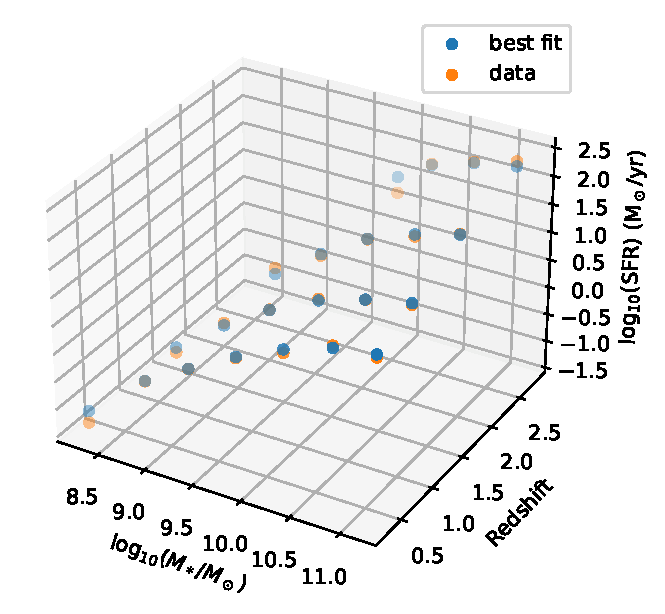
\includegraphics[trim={2cm 13.5cm 0.3cm 0.5cm},
  \includegraphics[width=0.65\linewidth]{Figs/Chapter3/2D_SFR_fit_data.pdf}
  \caption{A 2-dimensional plot of the SFR data for star forming galaxies from Chapter~\ref{ch:observations} as a function of ${\rm M}_*$ and redshift, compared with our best fit of Eq.~\ref{eq:SFR}.
  }
    \label{fig:SFR_2D_fit}
\end{center}
\end{figure*}
\begin{figure*}
%%%%%\vspace{8cm}
\begin{center}
  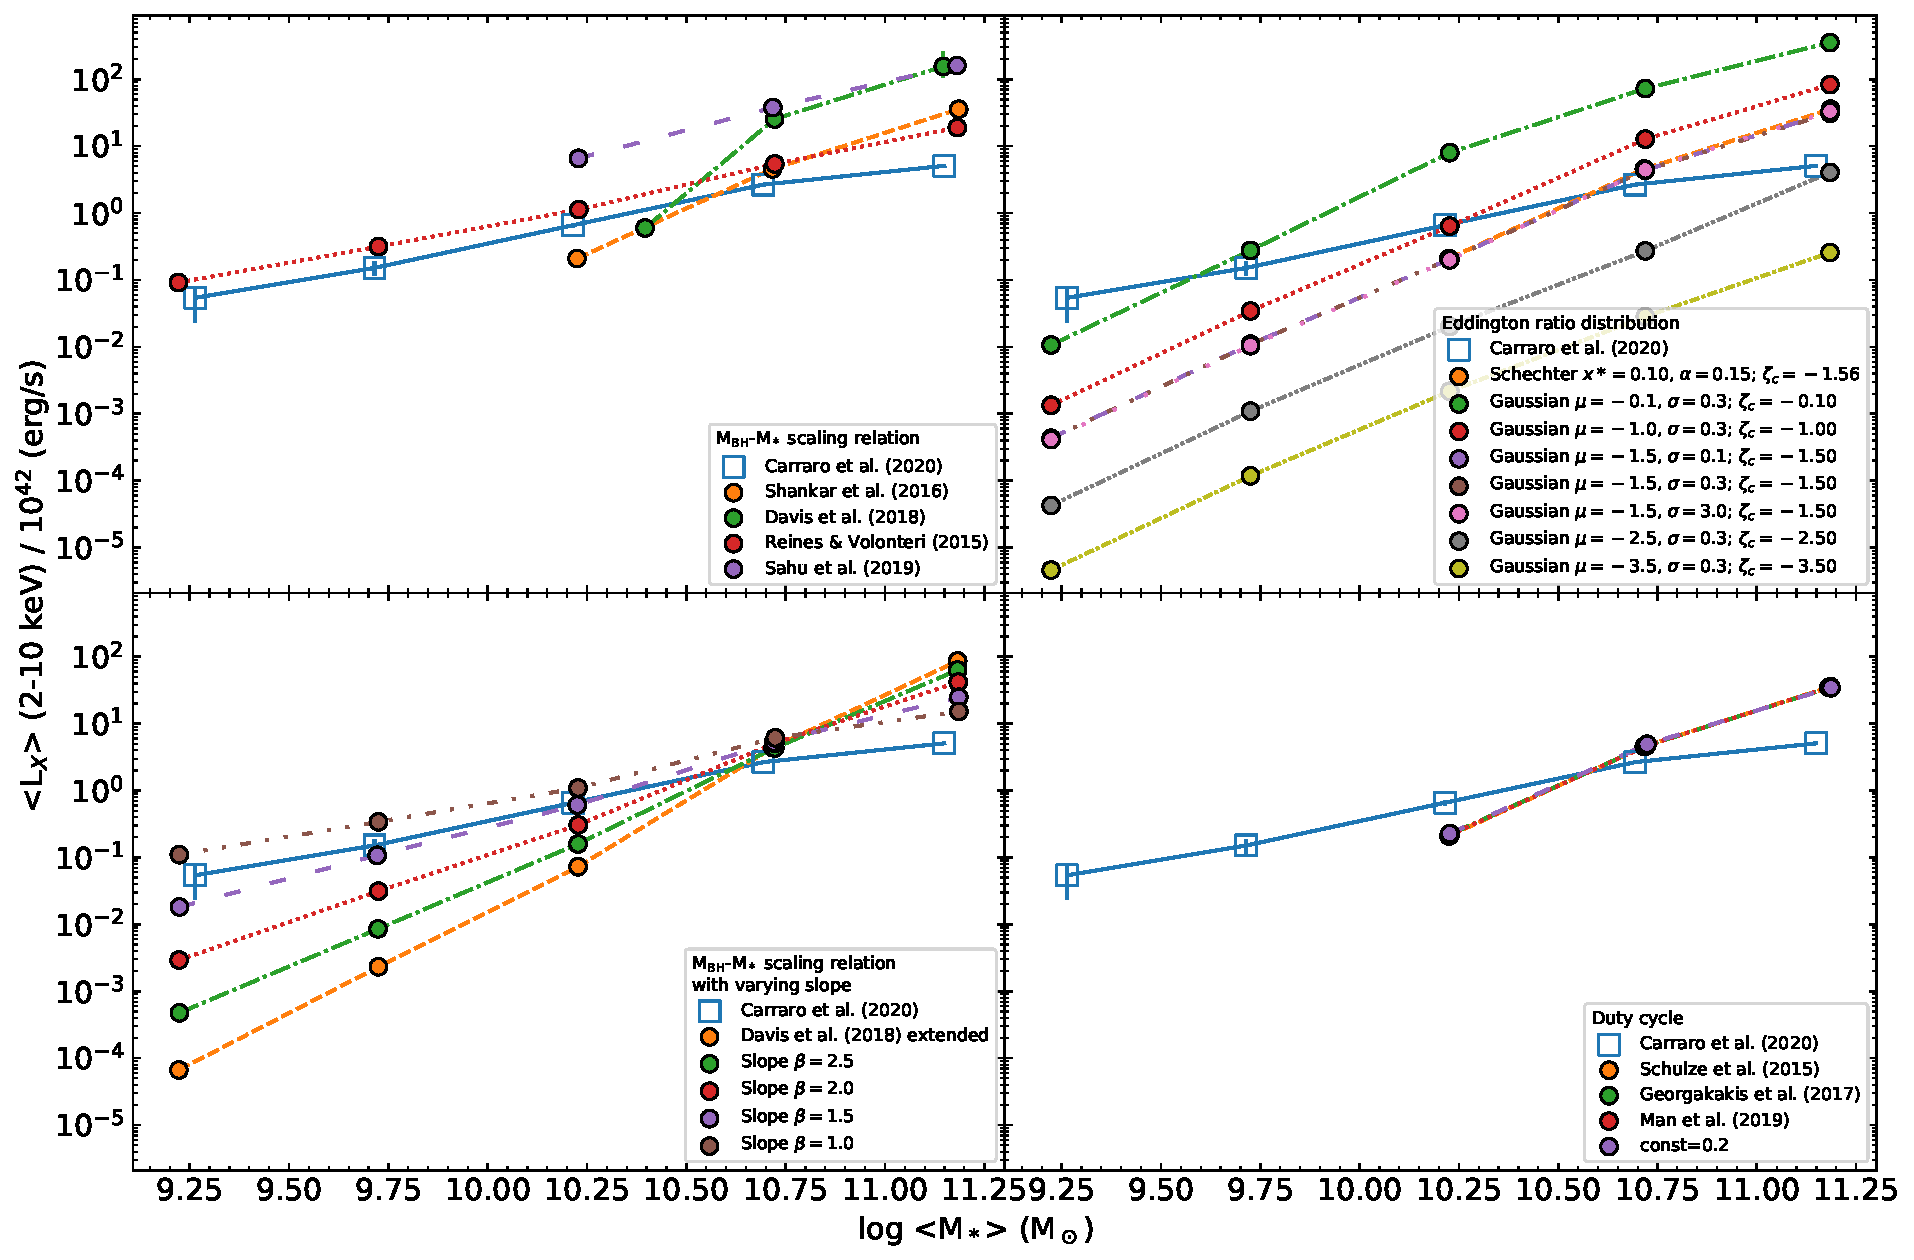
\includegraphics[width=\textwidth]{Figs/Chapter3/fig2_z1.0.pdf}
  \caption{A gallery of L$_{\rm X}-{\rm M}_*$ relations obtained by varying one of the input relations at a time. The relation that varies in each subplot is reported in the legend. 
  %Broken lines are added to the plot to guide the reader. All data-points are at $z=1$.
  Results from COSMOS data at $z=1$ from Chapter~\ref{ch:observations} (blue squares, see Fig.~\ref{fig:L_X}), are included in all plots for comparison.
  %All data-points are at $z=1$.
  Top left: L$_{\rm X}-{\rm M}_*$ relation obtained by changing the Eddington ratio distribution function. We use a Schechter function and Gaussian function in $\log(\lambda)$ with varying mean $\mu$ and standard deviation $\sigma$ values.
  Top right: L$_{\rm X}-{\rm M}_*$ relation obtained by changing the duty cycle method. Each M$_{\rm BH}-{\rm M}_*$ scaling relation is shown within its original stellar mass range of derivation.
  Bottom left: L$_{\rm X}-{\rm M}_*$ relation obtained by changing the M$_{\rm BH}-{\rm M}_*$ scaling relation.
  Bottom right: L$_{\rm X}-{\rm M}_*$ relation obtained with a toy M$_{\rm BH}-{\rm M}_*$ scaling relation where we change the logarithmic slope $\beta$ of the relation $\log {\rm M}_{\rm BH} = \alpha + \beta \log {\rm M}_*$.
  }
    \label{fig:LX_M}
\end{center}
\end{figure*}
Before computing the average X-ray luminosity we assign to each galaxy, irrespective of their duty cycle, an X-ray luminosity from X-ray binary emission following \citet[][Table 3]{2016ApJ...825....7L}, and then, as in Sec.~\ref{subsec:LX_BHAR}, subtract the mean binary emission competing to that bin of stellar mass and star formation rate. We note that neglecting X-ray binary emission entirely from our procedure would yield very similar results.
Following the procedure described above, we generate diverse galaxy mock catalogs with distinct choices of the input scaling relations, duty cycles, and $P(\log\lambda,z)$ distributions. 
We then divide each AGN mock catalog in bins of stellar mass, and perform 500 bootstraps out of which we extract the median SFR and M$_*$, and the linear mean L$_{\rm X}$ weighted by the AGN duty cycle %\log M_{BH,i}
\begin{equation}
\left<L_X\right>=\frac{\sum_i U_i(y_i,z) L_X(y_i)} {\sum_i U_i(y_i,z)}\, ,
    \label{eq:meanLx}
\end{equation}
where 
\begin{equation}
\log L_X(y_i) [erg\;s^{-1}]=38.1 +\log \lambda_i +y_i-\log k_X.
\label{eq:Lx_210}
\end{equation} 
For each bootstrapped distribution we compute the median SFR and $L_X$ and their 5th and 95th percentiles, following the same procedure as in the comparison observational sample Chapter~\ref{ch:observations}.



\section{Results}\label{sec:results}

\subsection{The effect of the model's inputs on the ${\rm L}_{\rm X}-{\rm M}_*$ relation} \label{ssec:Fig2}

To pin down the input parameters that mostly control the L$_{\rm X}-{\rm M}_*$ relation, we explore in Figure~\ref{fig:LX_M} how the relation varies by changing, from top left to bottom right, the $P(\log \lambda,z)$, the duty cycle, the full M$_{\rm BH}-{\rm M}_*$ relation, and only the slope of the \citet{2015ApJ...813...82R} relation, as labeled. 
All the mocks are generated at $z=1$, though the results are applicable at all redshifts, as further discussed below.

The top panels clearly show that whilst the normalization of the L$_{\rm X}-{\rm M}_*$ relation is strongly controlled by the characteristic Eddington ratio $\zeta_c$ (left), it has a negligible dependence on the AGN duty cycle (right). To note that a Schechter or Gaussian $P(\log \lambda,z)$ yield the same mean X-ray luminosity at fixed stellar mass as long as their $\zeta_c$ are the same (dotted green and dot-dashed red lines). The mean X-ray luminosity will be mostly controlled by the rate at which galaxies of a given BH/stellar mass are accreting and not by how many galaxies are active at any given time. The bottom panels of Figure~\ref{fig:LX_M} show instead a direct proportionality between the normalizations (left) and slopes (right) of the  M$_{\rm BH}-{\rm M}_*$ and the L$_{\rm X}-{\rm M}_*$ relations: a lower/shallower M$_{\rm BH}-{\rm M}_*$ scaling relation will result in a proportionally lower/shallower L$_{\rm X}-{\rm M}_*$ relation, and vice versa.

It is clear from Fig.~\ref{fig:LX_M} that the slope and normalization of the input M$_{\rm BH}-{\rm M}_*$ relation, as well as the input $\zeta_c$, all play a significant, and in fact degenerate, role in shaping the L$_{\rm X}-{\rm M}_*$ relation. For example, a flatter slope in the M$_{\rm BH}-{\rm M}_*$ relation or a mass-dependent $\zeta_c$, progressively decreasing at larger masses, could both produce a flatter slope in the L$_{\rm X}-{\rm M}_*$ relation. A decreasing $\zeta_c$ with increasing M$_{\rm BH}$ or ${\rm M}_*$  could indeed reconcile the observational results from Chapter~\ref{ch:observations} with a steeper M$_{\rm BH}-{\rm M}_*$ relation as calibrated in the local Universe \citep[e.g.,][]{2016MNRAS.460.3119S,2018ApJ...869..113D}. 

The results reported in Fig.~\ref{fig:LX_M} point to the L$_{\rm X}-{\rm M}_*$ relation as a powerful tool to constrain the mean rate of accretion of BHs $\zeta_c$ as a function of time and BH mass in ways independent of the duty cycle. 
As detailed in Eq.~\ref{eq:PhiL}, the AGN X-ray luminosity function is degenerate in BH mass function, duty cycle and $P(\lambda,z)$. However, independent constraints on $\zeta_c$ from the L$_{\rm X}-{\rm M}_*$ relation could then shed light on the duty cycle if a robust estimate of the underlying BH-galaxy scaling relation is available from, e.g., AGN clustering measurements \citep[see discussion in][]{ShankarNat,Allevato21}, or vice versa.

\subsection{The minor effect of $\lambda_{min}$ on our models}
We are considering in our mock catalogs galaxies with an Eddington ratio in the range $-4<\log(\lambda)<1$. This limit cannot be imposed in the selection of the observational sample for obvious reasons, but the effect of this choice of the minimum Eddington ratio $\lambda_{min}$ is negligible. In fact, we can extend the distribution of Eddington ratios down to ever lower $\lambda_{min}$ and still find very similar average X-ray luminosities, as long as the starting overall shape of the Eddington ratio distribution is not changed. This behavior simply stems from the fact that, to match the observational data, we are selecting in the mock catalogs galaxy stellar masses above ${\rm M}_*\ge 10^9 {\rm M}_\odot$, which tend to correspond to BH masses of the order of ${\rm M}_{\rm BH}\ge10^5 {\rm M}_\odot$, which in turn are mapped to (minimum) X-ray luminosities of the order of ${\rm L}\ge10^{38}erg/s$ (see Eq.~\ref{eq:Lx_210}).

Extending to even lower Eddington ratios produces proportionally lower X-ray luminosities that do not significantly contribute to the mean X-ray luminosity in any stellar mass bin considered in this work. In Fig.~\ref{fig:test_lambda_min} we show the predicted  relation when varying the $\lambda_{min}$ by 4 orders of magnitude, as labeled, but keeping fixed the overall shape of the input Eddington ratio distribution, BH-galaxy scaling relation and duty cycle. 
As expected, the average X-ray luminosity is nearly identical in all cases, as the minimum X-ray luminosities tend to be the same when keeping the same cuts in stellar mass.

\begin{figure*}
\begin{center}
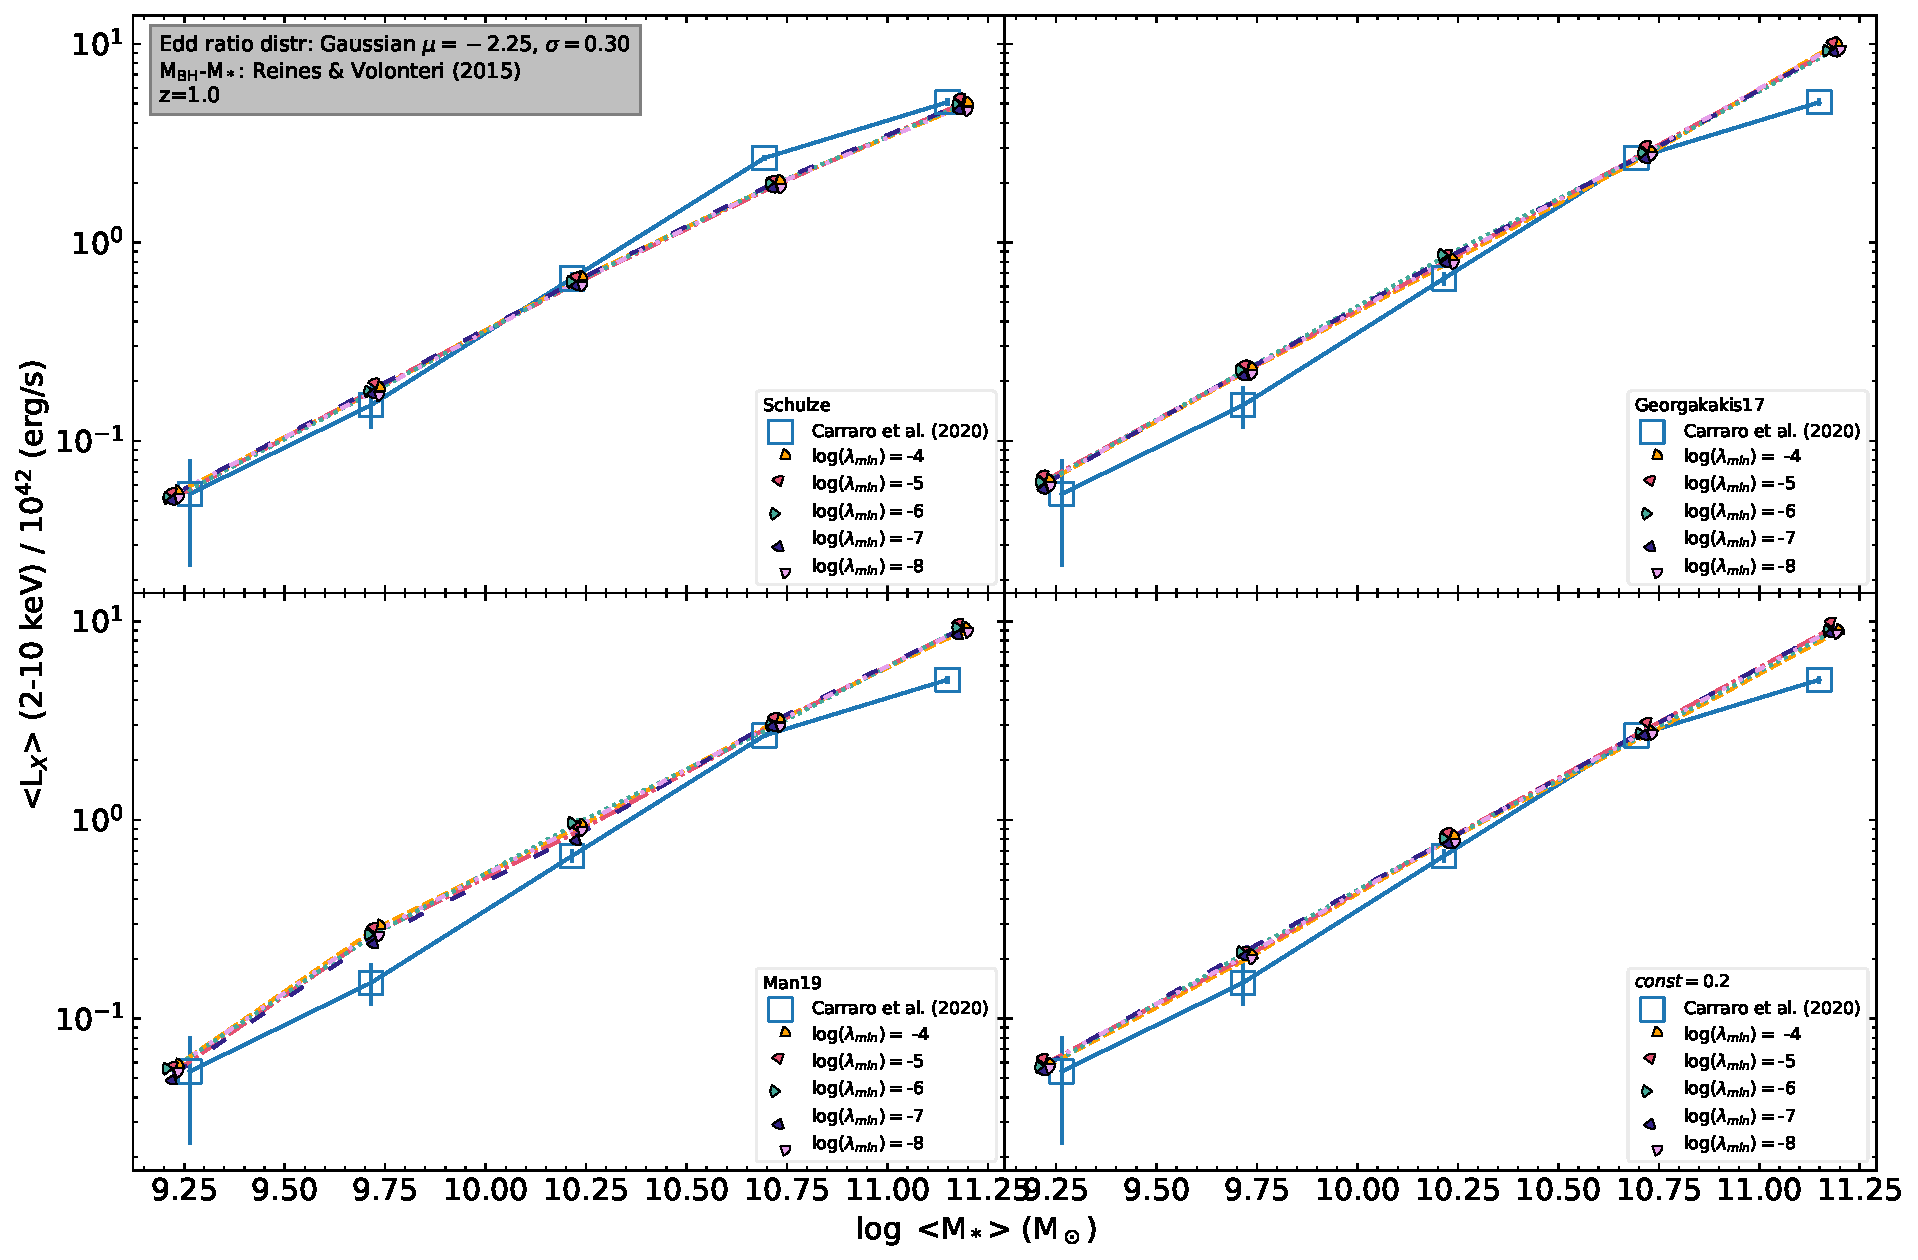
\includegraphics[width=\textwidth]{Figs/Chapter3/Test_lambda_min_z1.0.pdf} 
  \caption{L$_{\rm X}$ as a function of ${\rm M}_*$ for each of the duty cycles considered in this Chapter by varying the value of the minimum Eddington ratio, as labeled.}
    \label{fig:test_lambda_min}
\end{center}
\end{figure*}

\subsection{Reproducing the ${\rm L}_{\rm X}-{\rm M}_*$ relation through cosmic time}

In this Section we extend the comparison to data on the L$_{\rm X}-{\rm M}_*$ relation at different redshifts. The data point to a steady decrease of the mean ${\rm L}_{\rm X}$ luminosity with cosmic time at fixed host galaxy stellar mass. As discussed above, this decreasing trend could be interpreted either as a progressive decline in the normalization of the M$_{\rm BH}-{\rm M}_*$ relation and/or in the characteristic $\zeta_c$. The latest data suggest a rather weak evolution in the M$_{\rm BH}-{\rm M}_*$ relation up to at least $z\sim 2.5$ \citep[e.g.,][]{Suh20,Shankar20MNRAS} thus favoring, in our approach, a steady decrease in $\zeta_c$, which would also be in line with independent observations \citep[]{Kollmeier06} and continuity equation models \citep[][]{Shankar13Acc,Aversa15}.

In Figure~\ref{fig:LX_M_redshift} we show the L$_{\rm X}-{\rm M}_*$ relation for mock catalogs at $z=0.45,1.0,2.7$ (left, central and right panels respectively), generated by assuming as a reference the \citet{2015ApJ...813...82R} M$_{\rm BH}-{\rm M}_*$ relation, which naturally generates a slope in the L$_{\rm X}-{\rm M}_*$ relation, consistent with our data. 
 At each redshift we plot the models for two values of $\mu$ in $P(\log \lambda,z)$ (the corresponding $\zeta_c$ values are very similar being Gaussian distributions), roughly consistent with the higher and lower values of the L$_{\rm X}-{\rm M}_*$ relation.
We find that, assuming a strictly constant M$_{\rm BH}-{\rm M}_*$ relation, to reproduce the data we would need a drop of a factor of $\gtrsim 10$ in the characteristic Eddington ratio $\zeta_c$ from $z\sim 2.7$ to $z\sim 0.45$, which is broadly in line with some observational data and models' results \citep[see, e.g., Fig. 12 in][]{Shankar13Acc}. 

\begin{figure*}
%%%%%\vspace{8cm}
\begin{center}
  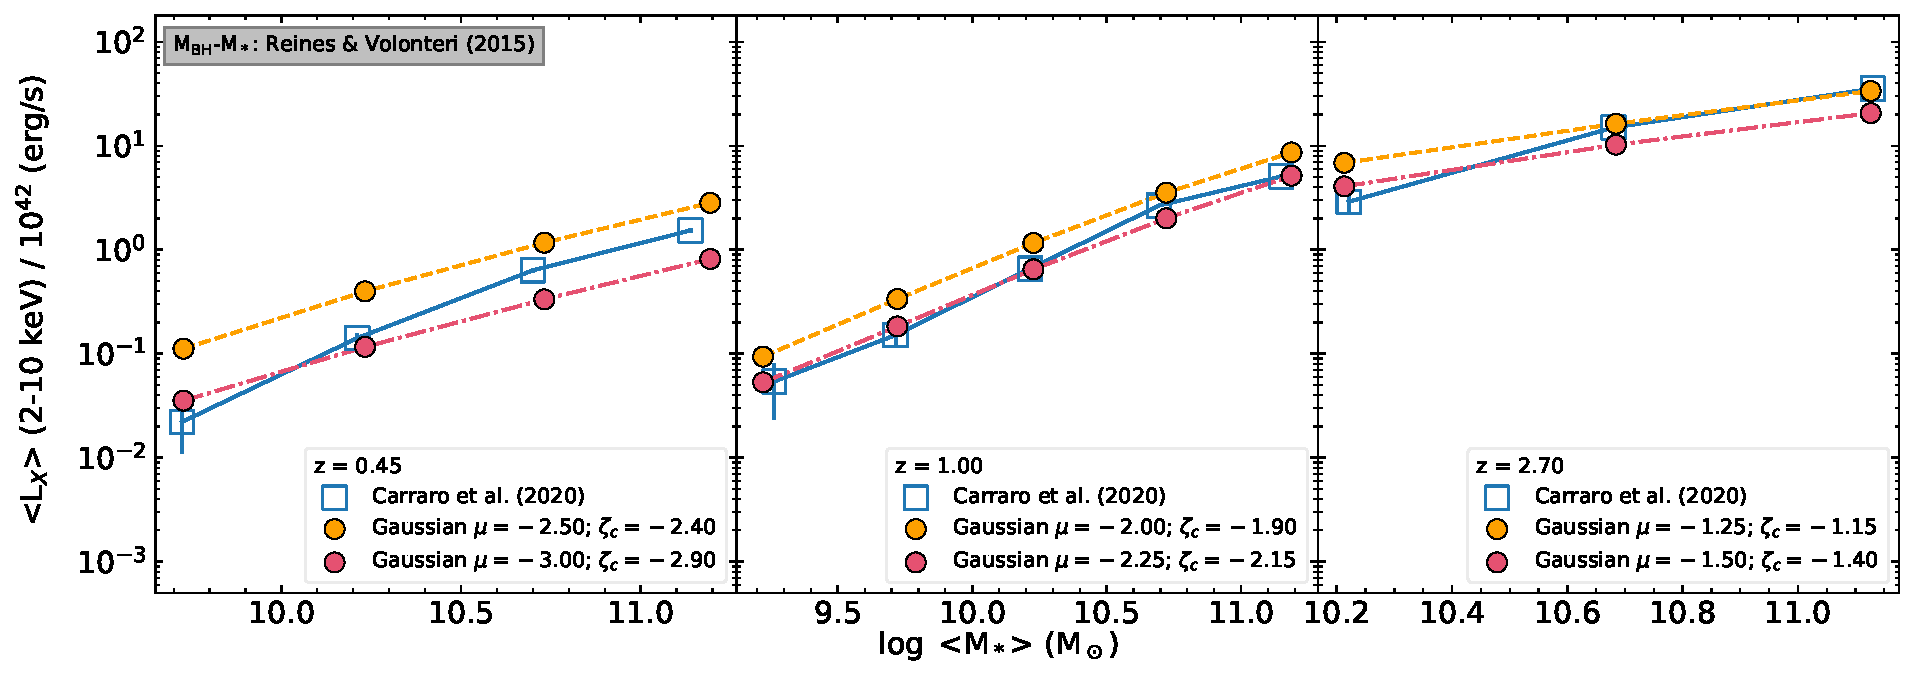
\includegraphics[width=\textwidth]{Figs/Chapter3/fig3.pdf}
  \caption{The L$_{\rm X}-{\rm M}_*$ relations at $z=0.45$ (left panels), $z=1.0$ (central panels) and $z=2.7$ (right panels) obtained by assuming a M$_{\rm BH}-{\rm M}_*$ scaling relation from \citet{2015ApJ...813...82R} and a Gaussian in $\log (\lambda)$ with standard deviation $\sigma=0.3$~dex. We vary the Eddington ratio distribution in order to reproduce the observational results from Chapter~\ref{ch:observations}. }

    \label{fig:LX_M_redshift}
\end{center}
\end{figure*}


\begin{figure*}
%%%%%\vspace{8cm}
\begin{center}
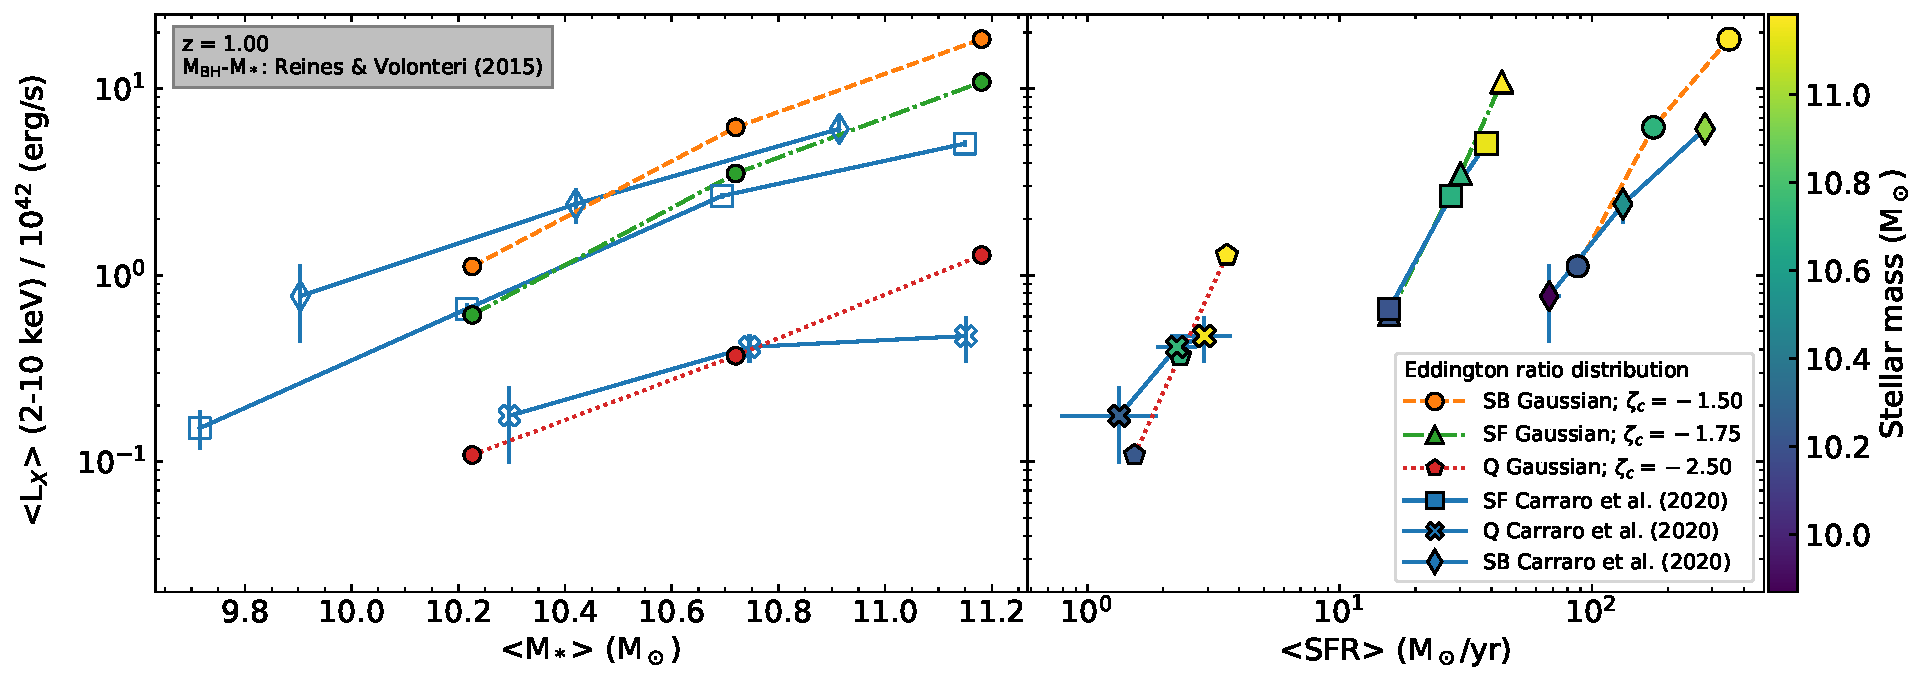
\includegraphics[width=\textwidth]{Figs/Chapter3/fig4.pdf} 
  \caption{L$_{\rm X}$ as a function of ${\rm M}_*$ (left) and SFR (right). L$_{\rm X}$ are obtained at $z=1$ with a \citet{2015ApJ...813...82R} M$_{\rm BH}-{\rm M}_*$ scaling relation and with a Gaussian Eddington ratio distribution as shown in the legend, with a $\sigma=0.3 dex$. In the right panel, SFRs are obtained using the fits from \ref{table:all_fitpar} for starburst (SB) and quiescent (Q) while the fit of Eq.~\ref{eq:SFR} is used for star-forming (SF) galaxies. Data points are color coded according to ${\rm M}_*$. All relations are compared with results from COSMOS data from Chapter~\ref{ch:observations}.}
    \label{fig:SFQSB}
\end{center}
\end{figure*}

\subsection{Reproducing the ${\rm L}_{\rm X}-{\rm M}_*$ relation in starburst, main-sequence and quiescent galaxies} \label{subsec:SFQSB}

In this Section we focus on the dependence of the ${\rm L}_{\rm X}-{\rm M}_*$ relation on galaxy type at fixed redshift, specifically $z=1$.
In Chapter~\ref{ch:observations} we showed in fact that, at least at $z<2.25$, starbursts, star forming and quiescent galaxies are characterized by distinct ${\rm L}_{\rm X}-{\rm M}_*$ relations, which are similar in slope but differ in normalization by a factor of $\sim 10$ when moving from quiescent galaxies, with the lowest average ${\rm L}_{\rm X}$, to the starbursts, with the largest average L$_{\rm X}$ at fixed stellar mass. 

In the left panel of Fig.~\ref{fig:SFQSB} we explore mocks with a constant input ${\rm M}_{\rm BH}-{\rm M}_*$ relation from \citet{2015ApJ...813...82R}, and a varying $\zeta_c$ (circles, triangles, and pentagons) against the different data sets for the three types of galaxies studied in Chapter~\ref{ch:observations} (blue diamonds, squares and crosses for starbursts, star forming, and quiescent galaxies respectively). Reproducing the steep increase in mean ${\rm L}_{\rm X}$ at fixed ${\rm M}_*$ requires, as expected, a proportionally higher value of $\zeta_c$ in star forming and starburst galaxies, assuming the same ${\rm M}_{\rm BH}-{\rm M}_*$ relation.

Interestingly, it is apparent from Fig.~\ref{fig:SFQSB} that the observed ${\rm L}_{\rm X}-{\rm M}_*$ relation is not a simple power law but tends to show a break that becomes more pronounced in more massive quiescent galaxies of mass $\log (M_*/M_{\odot}) \gtrsim 11$. In our modeling this feature could be naturally reproduced with a further decrease in $\zeta_c$ in the most massive and quiescent galaxies in our sample, which would align with the idea of downsizing, supporting the view that more massive galaxies and their central BHs have accreted their mass at a faster pace and are now in their declining phase. We stress that the downsizing in $\zeta_c$ would be even more pronounced if steeper M$_{\rm BH}-{\rm M}_*$ relations were adopted in input. The right panel of Fig.~\ref{fig:SFQSB} shows that our chosen values of $\zeta_c$ that match the ${\rm L}_{\rm X}-{\rm M}_*$ relation for each galaxy type also reproduce, at the same time, their respective ${\rm L}_{\rm X}-{\rm SFR}$ relations, where the SFR is assigned to each galaxy type based on their observed underlying ${\rm M}_*-{\rm SFR}$ relation.

An alternative way to explain the different normalizations of starburst and quiescent galaxies in the ${\rm L}_{\rm X}-{\rm M}_*$ plane would be to adopt the same $\zeta_c$ for all galaxy types and progressively increase the normalization of the M$_{\rm BH}-{\rm M}_*$ scaling relation when moving from quiescent to starburst galaxies.  
However, such a solution would not be favored from an evolutionary point of view as quiescent galaxies should be older galaxies with larger BHs at fixed stellar mass.

All in all, the evolutionary picture that could be extracted from Fig.~\ref{fig:SFQSB} is one in which the central BH and its host galaxy move around a similar M$_{\rm BH}-{\rm M}_*$ scaling relation throughout their lifetime. They could start from a main-sequence or even starburst, gas-rich phase, evolving at an almost constant (specific) SFR, as also proposed by theoretical models \citep[e.g.][]{2014ApJ...782...69L, Aversa15} and direct observations (Chapter~\ref{ch:observations}), and then gradually switch off their accretion and star formation due to internal gas consumption, thus gradually reducing their SFR and accretion onto the central BH (right panel of Fig.~\ref{fig:SFQSB}).  

\section{Discussion and conclusions}\label{sec:disc_concl}
In this Letter we use statistical semi-empirical models to generate accurate mock catalogs of active galaxies, which we analyze in the same manner as in the comparison observational sample from Chapter~\ref{ch:observations}. Our goal is to unveil the input parameters driving the L$_{\rm X}-{\rm M}_*$ relation. We start from a halo mass function at a given redshift, we assign galaxies and BHs to dark matter haloes via the most up-to-date empirical stellar-halo and M$_{\rm BH}-{\rm M}_*$ relations and we assume a SFR depending only on stellar mass and redshift. We explore a range of Eddington ratio distributions, M$_{\rm BH}-{\rm M}_*$ scaling relations and duty cycles.

We show that the L$_{\rm X}$-SFR or L$_{\rm X}-{\rm M}_*$ is largely independent of the AGN duty cycle, but strongly depends on the shape of the M$_{\rm BH}-{\rm M}_*$ scaling relation and on the characteristic Eddington ratio $\zeta_c$, linking the mean L$_{\rm X}$ with the M$_{\rm BH}$. The L$_{\rm X}-{\rm M}_*$ relation can break degeneracies among input duty cycles, Eddington ratio distributions and also BH-galaxy scaling relations, especially when the latter are coupled with AGN clustering measurements \citep{ShankarNat}, thus representing a powerful tool for cosmological models. 
We find that our current data on L$_{\rm X}-{\rm M}_*$ favor, at fixed $\zeta_c$, flatter M$_{\rm BH}-{\rm M}_*$ relations, or M$_*$-dependent $\zeta_c$ for steeper M$_{\rm BH}-{\rm M}_*$ relations. An M$_*$-dependent $\zeta_c$ combined with a steeper M$_{\rm BH}-{\rm M}_*$ relations would indeed be favored by different observational studies \citep[][and Fig.~\ref{fig:comp_models}]{2019ApJ...885L..36D, 2019MNRAS.484.4360A}, continuity equation arguments \citep{Shankar13Acc,Aversa15} and population synthesis models \citep{2018MNRAS.476..436B}. We checked that by fitting the observed L$_{\rm X}-{\rm M}_*$ at $z=1$ with a $P(\log \lambda, z)$ distribution with a characteristic $\zeta_c\simeq-2.15$, is nicely consistent with the mean specific BH accretion rate $\lambda_{sBHAR}$ measured by \citet{2019MNRAS.484.4360A} from large samples of deep X-ray AGN surveys.

In our previous Chapter, see e.g. Fig.~\ref{fig:SF_BH_all}, we showed that main-sequence and quiescent galaxies share similar ratios of BHAR and SFR at all probed cosmic epochs, suggesting that the two processes are linked together throughout different galaxy phases.  
In fact, the mean BHAR/SFR can be written as ${\rm BHAR/SFR} \propto L_{bol}/{\rm SFR} \propto 10^{\zeta_c} {\rm M}_{\rm BH}/(k {\rm M}_*)$, where $k={\rm SFR}/{\rm M}_*$ is the specific SFR. Thus, at fixed ${\rm M}_{\rm BH}/{\rm M}_*$, a similar BHAR/SFR ratio as the one observed in star forming and quiescent galaxies, would be induced by a proportional decline in characteristic Eddington ratio $\zeta_c$ and specific SFR $k$ within a bin of stellar mass. Analogously, the significantly lower BHAR/SFR in starbursts with respect to quiescent/star forming galaxies as measured in Chapter~\ref{ch:observations}, would be naturally interpreted as a proportionally higher specific SFR $k$ %and roughly constant $\zeta_c$ throughout the star formation phase, as predicted by some BH evolution models \citep[e.g.,][]{Aversa15}.
and roughly constant or slightly higher $\zeta_c$ in these young gas rich systems, as predicted by some BH evolution models \citep[e.g.,][]{Aversa15}.
\clearchapterpage
%%=+=+=+=+=+=+=+=+=+=+=+=+=+=+=+=+=+=+=+=+=+=+=+=+=+=+=+=+=+=+=+=+
%
%%###### CHAPTER 4 #######
%%++++++++++++++++++++++++++++++++++++++++++++++++++++++++++++++++
\chapter{Optical-IR variability in AGN}

%\begin{center}
%  {\it ``If could add an introductionary text here.''}
%  \vspace{1cm}
%\end{center}


\section{Observations}
\subsection{Sample selection}
\subsection{Observation campaign with SMARTS 1.3m ANDICAM} \label{ssec:obs_strategy}
\section{Methods}
\subsection{Optical light curves extraction}
\subsection{IR light curves extraction}
\subsection{Cross correlation and significance}
\section{Results}
\subsection{Lags}
\subsection{Variability spectrum}
\section{Discussion}
\subsection{Comparison with predictions from Shakura-Sunyaev disk model and dusty torus}

\section{Conclusions}
%\begin{figure}[t]
%\begin{center}
%  \includegraphics[scale=0.5, angle=-90]{photo.png}
%  \caption{Here you can provide the caption.}
%    \label{and_the_label}
%  }
%\end{center}
%\end{figure}

\clearchapterpage
%%=+=+=+=+=+=+=+=+=+=+=+=+=+=+=+=+=+=+=+=+=+=+=+=+=+=+=+=+=+=+=+=+
%
%%###### CHAPTER 5 #######
%%++++++++++++++++++++++++++++++++++++++++++++++++++++++++++++++++

\chapter{Estimating the gas distribution in AGN nuclei} \label{ch:gas_distribution}

%\begin{center}
%  {\it ``If could add an introductionary text here.''}
%  \vspace{1cm}
%\end{center}


\section{Intro}
X-ray emission is a universal characteristic of Active Galactic Nuclei (AGN), thought to arise from inverse Compton upscattering of optical/UV photons of the accretion disk by hot electrons in the corona  \citep[e.g.,][]{1991ApJ...380L..51H}. The intrinsic X-ray emission takes a power-law spectral form  [$f(E){\propto}E^{-\Gamma}$, with  typical photon indices of ${\langle}\Gamma{\rangle}{\sim}1.8$--$2.0$; e.g., \citealt{1994MNRAS.268..405N, 2009ApJ...690.1322W, 2011A&A...530A..42C}], but can be modified due to interaction with matter in the vicinity of the central Supermassive Black Hole (SMBH). In particular, Compton scattering and photoelectric absorption of the primary X-ray continuum lead to two important features in the X-ray spectrum: the \kalfa{} emission line and the so-called "Compton-hump". By studying these reprocessed features, together known as the so-called AGN "reflection" component, we can infer the physical properties of the matter from which they originate, and hence probe the circumnuclear environments of central SMBHs. These physical emissions have to be studied through spectral analysis, as X-ray data do not have enough resolution to allow us to directly observe the very small $\sim pc$ scales where these processes take place, so an indirect approach is needed.

The \kalfa{} line at 6.4 keV is produced by fluorescence processes related to the absorption of higher energy X-ray photons by neutral Fe atoms. Its spectral profile is generally comprised of broad and narrow components. The narrow component of the \kalfa{} line \citep[
$\rm FWHM {\lesssim} 10,000\:km\:s^{-1}$; e.g.,][]{2001MNRAS.323L..37L,2004ApJ...604...63Y,2010ApJS..187..581S} is an ubiquitous spectral feature of AGN, and in a majority of cases the only component present, while the broad component is harder to pin down since it requires exceptional statistics and broad energy coverage to decouple the line from the underlying continuum and absorption components \citep[e.g.,][]{2006AN....327.1032G, 2014ApJ...787...83M}.
Nonetheless, when present, reverberation studies suggest that the broad component originates from a compact zone, only a few $r_g$ in extent, around the SMBH \citep[e.g.,][]{2014MNRAS.438.2980C}, and hence is strongly affected by Doppler and gravitational broadening \citep[e.g.,][]{1995MNRAS.272L...9M,1995Natur.375..659T,1995ApJ...453L..81Y}. On the other hand, the narrow component is thought to be produced somewhere among the outer accretion disk, the broad line region (BLR) and the torus clouds \citep[e.g.,][]{1994MNRAS.267..743G,1994ApJ...420L..57K,1995ApJ...453L..81Y}, corresponding to light month-to-year distances. 

Rapid X-ray continuum variability is commonly observed in unobscured, obscured, and even some heavily obscured AGN and suggests that the primary X-ray emitting source (i.e., the corona) is produced in a compact zone very near to the SMBH \citep[e.g.,][]{1993ARA&A..31..717M, 2013MNRAS.431.2441D}. The X-ray light curve can be analyzed via the power spectral density (PSD) function, which is typically characterized as a power law of the form $P_{\nu} \propto \nu ^{\alpha}$, where $\nu = 1/T$ is the frequency and $\alpha$ is the power law slope \citep[e.g.,][]{1993MNRAS.265..664G, 1999ApJ...514..682E, 2003MNRAS.339.1237V}. Typical values for the power law slope in AGN are $\alpha{\sim}{-}1$ at lower frequencies, indicative of pink noise, and $\alpha\gtrsim-2$ at higher frequencies, indicative of red noise. The break in the PSD between these two regimes is denoted as $\nu_B = 1/T_B$, and is related to the characteristic X-ray variability timescales of the system. 

If we assume that the \kalfa{} line emission is reprocessed from the same X-ray continuum we observe, we can expect the \kalfa{} line flux tracks the continuum fluctuations. The light curves of both, primary and reflected components, can still differ by light travel time effects, as the reflected light can travel different and in general longer paths to the observer. The \kalfa{} line light curve can therefore be delayed with respect to the continuum and can also be smoothed out, as variations on timescales shorter than the light crossing time of the reflector are damped. The reduction of variability amplitude of the \kalfa{} line light curve with respect to the continuum, however, can shed light on the size of the reflector, as larger reflectors suppress a larger fraction of the intrinsic variance. The aim of this Chapter is to take advantage of this correlation between primary and reflected component by using temporal considerations and the variability properties to measure the size of the reflector. We did so in a sample of AGN from the work of Andonie et al. (in prep.) by simulating X-ray light curves and comparing their reduction in variability amplitude with the observed ones.

\section{Sample and data}
The AGN sample in this Chapter was presented in Carolina Andonie's master thesis. Onto this same sample we are performing an additional work which will be presented in Andonie et al. (in prep.). The sample was chosen to study the spectral and temporal properties of the \kalfa{} line in AGN, and was selected from the parent input sample the most recent 105-month \textit{Swift}-Burst Alert Telescope (BAT) Survey \citep{2018ApJS..235....4O}, an all-sky survey in the ultra-hard X-ray band (14--195 keV), which provides a relatively unbiased AGN sample at least up to $N_{\rm H}{\gtrsim}10^{24}\:cm^{-2}$ \citep{2015ApJ...815L..13R}. The 105-month Swift-BAT catalog is a uniform hard X-ray all-sky survey with a sensitivity of $8.4 {\times} 10^{-12}\: {\rm erg\:s^{-1}\:cm^{-2}}$ over $90\%$ of the sky in the 14–195 keV band. The survey catalogs 1632 hard X-ray sources, 947 of which are securely classified as AGN but the sample is reduced in order to include only sources with enough multiple observations from either Chandra or XMM. They include one additional target in their sample, the well-known narrow-line Sy1 1H0707$-$495, which is relatively bright in the 2--8\,keV band, yet somehow remains undetected in the BAT 105-month catalog.

Andonie et al. focus on observations in the 2-8 keV band where the \kalfa{} line is located, and use data from \textit{Chandra} \citep{2000SPIE.4012....2W} and \textit{XMM-Newton} \citep{2001A&A...365L...1J} which have a good sensitivity in this band. \textit{XMM-Newton} observations provide better spectral and timing statistics, but suffer from substantial background flaring.
On the other hand, \textit{Chandra} observations are more versatile since they offer high spatial resolution to search for extended \kalfa{} emission on $\sim$100-pc to kpc scales, and, when the High Energy Grating is deployed, sufficient spectral resolution to resolve the \kalfa{} line.

The authors limit their analysis only to those observations for which there is a high likelihood of constraining the \kalfa{} line, and apply a flux cut of $f_{\rm 14-195\: keV} \geqslant  10^{-11}\: {\rm erg\:s^{-1}\:cm^{-2}}$ and/or $f_{\rm 2-8\: keV} \geqslant  4\times 10^{-12} \: {\rm erg\:s^{-1}\:cm^{-2}}$ (these are roughly equivalent for a $\Gamma{=}1.9$ power law); this resulted in the selection of 252 sources in the local universe ($z<0.1$), and 28 more distant galaxies with redshifts between 0.1 and 0.56.

We simulate X-ray light curves for those galaxies which have determined PSD function parameters from either \citet{summons_thesis}, from long term monitoring campaigns performed with the Rossi X-Ray Timing Explorer (RXTE) observatory, or from \citet{2012A&A...544A..80G} (\citetalias{2012A&A...544A..80G} hereafter), from ...?. For the rest, we estimated the break frequency using the expression
\begin{equation}
    \log(T_b)=1.09\log(M_{BH}) + -0.24\log(L_{bol}) - 1.88
    \label{Eq:T_b}
\end{equation}
from \citetalias{2012A&A...544A..80G}, where $T_b$ is the PSD bending timescale ($T_b = 1/\nu_{b}$), $M_{BH}$ is the black hole mass in $10^6\:\rm M_{\odot}$ units, and  $L_{bol}$ is the bolometric luminosity in $10^{44}\:\rm erg\:s^{-1}$ units.

The final sample for which we are able to simulate X-ray light curves is composed of 33 sources which have between 2--68 observations in a time range between ... days. A complete list of the sources, their PSD parameters and observations is reported in Table \ref{tab:gals_obs_par}.

\section{Variability definitions} \label{sec:variability_defs}
The light curves obtained by Andonie el al. are too sparsely sampled to detect a delay between continuum and Fe line fluctuations, therefore we rely on estimating the reduction in variability amplitude. This can be quantified by calculating the ratio between the excess variance of the continuum ($\sigma^2_{\rm ct}$) and \kalfa{} line ($\sigma^2_{\rm Fe}$) light curves, as %$\xi_{r}=\sigma^2_{\rm Fe}/\sigma^2_{\rm ct}$.
\begin{equation}\label{eq:xi}
    \xi_{r}=\frac{\sigma^2_{Fe}}{\sigma^2_{ct}}.
\end{equation}\label{eq:xi}
The normalized excess variance ($\sigma^2$) \citep[e.g.,][]{1997ApJ...476...70N,2004ApJ...611...93P,2008A&A...487..475P} is a quantitative measurement of the variability amplitude of a light curve, and is defined as
\begin{equation}
\label{eq:NXS}
    \sigma^2_{rms} = \frac{1}{N_{obs}\overline{x}^2} \sum^{N_{obs}}_{i=1} [(x_i-\overline{x})^2-\sigma^2_{err,i}]
\end{equation}
while its error due to Poison noise is
\begin{equation}
\label{eq:NXS_err}
 err( \sigma^2_{rms}) = \frac{1}{N_{obs}^{3/2}\overline{x}^2} \sum^{N_{obs}}_{i=1} ([(x_i-\overline{x})^2-\sigma^2_{err,i}]-\sigma^2_{rms} \overline{x}^2)^2\,.
\end{equation}
The $\sigma^2_{rms}$ estimates the intrinsic variance of the light curve, normalized by its mean flux, to produce a dimensionless quantifier that can be easily compared between objects of different brightness or light curves from  different energy bands. The last term in Eq.~\ref{eq:NXS} estimates the contribution of the observational Poisson noise to the total variance, in order to subtract it, and the error formula in Eq.~\ref{eq:NXS_err} estimates the uncertainty in this subtraction. 

The excess variances and their ratios were estimated by running Monte Carlo simulations in order to quantify their variability robustly. 
These simulations are only aimed at quantifying how the observational Poisson noise affects the estimate of the $\sigma^2_{rms}$. For this purpose we add Gaussian noise to each light curve point, with a $\sigma$ equal to the error on the flux of each point. In this way, each simulation has the intrinsic variance of the light curve and twice the observational noise and allows to estimate the excess variance and its asymmetric uncertainties for each light curve.

Low intrinsic variances compared to the Poisson noise can sometimes lead to negative values of the $\sigma^2_{rms}$ estimate, since the uncertainty in the Poisson noise can be larger than the difference in Eq.~\ref{eq:NXS}. We will consider light curves as significantly variable if the lower 16\% bound of the excess variance distribution is positive. Table \ref{tab:gals_obs_par} shows the median and the 16\% and 84\% bounds of the ratio distributions of the excess variance of each light curve. These data are also plotted in Fig.~\ref{fig:exvars}. 

Significant variability (i.e. positive lower bound on the $\sigma^2_{rms}$ ) is detected in the continuum of all objects except for 4C+29.30.  Significant Fe K$\alpha$ line variability is detected in 2MASXJ23444387, 4C+74.26, Cen A, Circinus galaxy, IC4329A, MR2251-178, MRK 1040, MRK 1210, MRK 3, NGC 1068, NGC 1275, NGC 1365, NGC 253, NGC 2992, NGC 3783, NGC 4151, NGC 4388, NGC 6300 and NGC 7582. In many objects, however, the variability of the Fe K$\alpha$ line is consistent with the observational noise, within its uncertainties. This is the case for all objects for which the lower bound on the Fe K$\alpha$ line excess variance is negative. The upper bounds on the Fe K$\alpha$ line variability in those objects is still of interest, depending on how this bound compares to the variance of the continuum.

If the Fe K$\alpha$ line flux tracks the fluctuations of the continuum flux, then we expect their variances to be related. The ratio of the variances $\xi$ should be similar to 1 if the reflector is small compared to the timescale of the fluctuations, and smaller than 1 if the reflector is large. Therefore, upper bounds smaller than 1 in the ratio column of Table~\ref{tab:gals_obs_par} can allow us to place a lower limit on the size of the reflector. This is true for example in the first two objects in the table. Even though their Fe K$\alpha$ line variance is not significant, its upper limit is so far below the variance of the continuum that a lower limit can be placed on the size of the reflector, because if the reflector was any smaller, the Fe K$\alpha$ line variability would be detectable. Conversely, lower bounds of the variance ratio $\xi>0$ can put upper limits on the reflector size. One or both of these limits are therefore measurable in many objects in the table. We describe this analysis below in Sec.~\ref{sec:LC_sims}.

%The normalized excess variance of the continuum is generally well constrained. The median values of the $\sigma^2_{rms}$ distributions range from 0.006 for 3C 445 to 9.99 for 2MASXJ11315154-1231587. This large difference can raise doubts about a common origin of the continuum variability in all sources. We know however, from dedicated monitoring campaigns of radio-quiet AGN, that the X-ray power spectra of different AGN is remarkably uniform in shape and normalization, but that the timescale of the break in the power spectrum scales linearly with black hole mass and and inversely with accretion rate \citep{2006Natur.444..730M}. Since the excess variance equals the integral of the power spectrum over the timescales covered by the light curves, we can expect to measure significantly different values for objects of different black hole mass, even if the light curves have similar lengths.  

%To test how unusual some of these excess variances are, we computed the expected variance, for the respective BH masses and accretion rates. Since the variability is a stochastic process, and the underlying powerspectral shape is only realized on average, simulations provide a good way of estimating the possible range of variance measurements, for given BH parameters and light curve sampling pattern. 

\begin{figure*} 
 \centering
 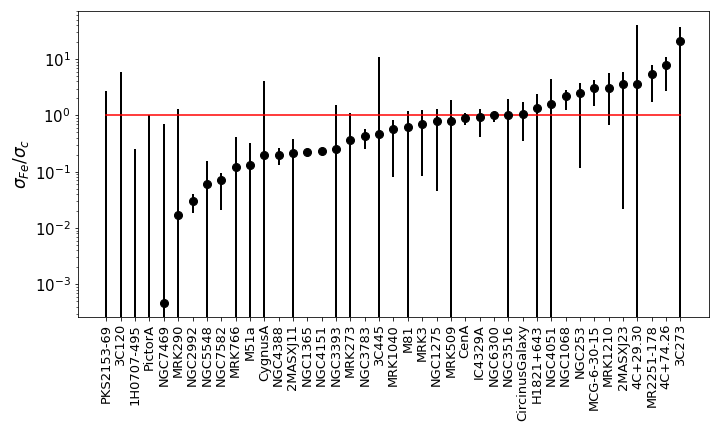
\includegraphics[width=\textwidth]{Figs/Chapter5/ratio_1s.png}
 %\captionsetup{width=1.5\linewidth}  
 \caption{The ratio between the normalized excess variance of the Fe K$\alpha$ line and continuum light curves $\xi=\sigma_{Fe}/\sigma_{ct}$. The error bars correspond to the 16$\%$ and 84$\%$ bounds of the normalized excess variance distributions.}\label{fig:exvars}
 \end{figure*} 

% USEFUL COMMENTS, DO NOT ERASE:
%Source                 & $\xi(50\%)_{16\%}^{84\%}$        & $\log{\rm M}_{\rm BH}$ & $\log L_{bol}$& $\nu_b$ & $\nu_b$  & $\alpha_h$ & Ref. & N Obs & Duration\\
%                       &              & $(\rm M_\odot)$ & (erg/s) & (Hz)    & (days$^{-1}$) & & & & (days) \\
% \caption{The galaxy sample from Andonie et al. (in prep.), its observations and its PSD parameters. Median $\xi$ parameters are reported with the 16\% to 84\% bounds of the distributions of normalized excess variance. Black hole masses are from Bass collaboration. $\nu_b$ and $\alpha_h$ (if available) are shown with the work they was extracted from and, whenever not available, the $\nu_b$ estimation with Eq.~\ref{Eq:T_b} is shown.}\label{tab:gals_obs_par}
%\specialcell{2MASXJ11315154\\-1231587}
\begin{footnotesize}%small
\begin{longtable}{llrrllrlrr}
\toprule
Source                 & $\xi(50\%)_{16\%}^{84\%}$        & $\log{\rm M}_{\rm BH}$ & $\log L_{bol}$& $\nu_b$ & $\nu_b$  & $\alpha_h$ & Ref. & N Obs & Duration\\
                       &              & $(\rm M_\odot)$ & (erg/s) & (Hz)    & (days$^{-1}$) & & & & (days) \\
\midrule
\endhead
\midrule
\multicolumn{10}{r}{{Continued on next page}} \\
\midrule
\endfoot

%\bottomrule
\endlastfoot
1H0707-495             &   $ -0.18_{-0.82}^{0.28} $ &             - &       - & $3.98\cdot10^{-4}$ &          34. &      2.4 &  {\citetalias{2012A&A...544A..80G}} &    14 &     6929 \\
\specialcell{2MASXJ11315154\\-1231587} &   $ 0.20_{-0.026}^{0.39} $ &          8.81 &    46.6 & $6.22\cdot10^{-7}$ &        0.054 &        - &                    Eq.~\ref{Eq:T_b} &    41 &     4990 \\
3C120                  &      $ -1.3_{-19.}^{6.6} $ &          7.74 &    45.2 & $7.83\cdot10^{-6}$ &         0.68 &        - &                    Eq.~\ref{Eq:T_b} &    11 &     4879 \\
3C273                  &       $ 18._{-17.}^{36.} $ &          8.84 &    47.0 & $7.30\cdot10^{-7}$ &        0.063 &        - &                    Eq.~\ref{Eq:T_b} &    47 &     6595 \\
4C+29.30               &       $ 3.8_{-27.}^{40.} $ &          8.28 &    44.9 & $1.28\cdot10^{-6}$ &         0.11 &        - &                    Eq.~\ref{Eq:T_b} &     6 &     3245 \\
4C+74.26               &        $ 7.7_{2.1}^{11.} $ &          9.83 &    46.0 & $2.00\cdot10^{-8}$ &       0.0017 &        - &                    Eq.~\ref{Eq:T_b} &     6 &     1571 \\
CenA                   &      $ 0.92_{0.66}^{1.1} $ &          7.77 &    43.1 & $2.26\cdot10^{-6}$ &         0.20 &        - &                    Eq.~\ref{Eq:T_b} &    39 &     6581 \\
CircinusGalaxy         &       $ 1.1_{0.33}^{1.8} $ &          6.23 &    43.5 & $1.07\cdot10^{-4}$ &          9.3 &      2.1 &  {\citetalias{2012A&A...544A..80G}} &    18 &     5006 \\
CygnusA                &     $ -0.51_{-6.0}^{3.7} $ &          9.43 &    45.6 & $5.30\cdot10^{-8}$ &       0.0046 &        - &                    Eq.~\ref{Eq:T_b} &    68 &     6209 \\
IC4329A                &      $ 0.99_{0.47}^{1.3} $ &          7.81 &    45.0 & $5.85\cdot10^{-6}$ &         0.51 &        - &                    Eq.~\ref{Eq:T_b} &    13 &     6222 \\
M81                    &     $ 0.75_{-0.24}^{1.2} $ &          7.90 &    39.5 & $2.13\cdot10^{-7}$ &        0.018 &        - &                    Eq.~\ref{Eq:T_b} &    38 &     6157 \\
MCG-6-30-15            &        $ 3.0_{1.5}^{4.2} $ &          6.14 &    43.9 & $3.80\cdot10^{-5}$ &          3.3 &      1.9 &            {\citet{summons_thesis}} &    12 &     4589 \\
MR2251-178             &        $ 5.3_{2.0}^{7.9} $ &          8.20 &    45.8 & $2.50\cdot10^{-7}$ &        0.022 &      2.5 &            {\citet{summons_thesis}} &    12 &     5489 \\
MRK1040                &     $ 0.57_{0.18}^{0.82} $ &          7.41 &    44.6 & $1.55\cdot10^{-5}$ &          1.3 &        - &                    Eq.~\ref{Eq:T_b} &     8 &     4770 \\
MRK1210                &       $ 3.4_{0.90}^{6.1} $ &          6.76 &    44.3 & $9.94\cdot10^{-5}$ &          8.6 &        - &                    Eq.~\ref{Eq:T_b} &     7 &     2496 \\
MRK273                 &     $ 0.43_{-0.90}^{1.0} $ &          8.78 &    44.1 & $1.78\cdot10^{-7}$ &        0.015 &        - &                    Eq.~\ref{Eq:T_b} &     8 &     6149 \\
MRK290                 &      $ 0.13_{-1.7}^{1.4} $ &          7.28 &    44.4 & $2.06\cdot10^{-5}$ &          1.8 &        - &                    Eq.~\ref{Eq:T_b} &     8 &     1042 \\
MRK3                   &      $ 0.73_{0.12}^{1.3} $ &          6.72 &    44.8 & $1.51\cdot10^{-4}$ &          13. &        - &                    Eq.~\ref{Eq:T_b} &    19 &     5511 \\
MRK509                 &     $ 0.76_{-0.81}^{1.8} $ &          8.05 &    45.3 & $7.60\cdot10^{-8}$ &       0.0066 &      1.5 &            {\citet{summons_thesis}} &    18 &     4335 \\
MRK766                 &    $ 0.11_{-0.35}^{0.43} $ &          6.60 &    43.9 & $2.90\cdot10^{-4}$ &          25. &      2.9 &            {\citet{summons_thesis}} &    11 &     5172 \\
NGC1068                &        $ 2.3_{1.4}^{2.8} $ &          6.93 &    43.9 & $4.81\cdot10^{-5}$ &          4.2 &        - &                    Eq.~\ref{Eq:T_b} &    12 &     5301 \\
NGC1275                &     $ 0.82_{0.025}^{1.3} $ &          7.55 &    45.1 & $1.38\cdot10^{-5}$ &          1.2 &        - &                    Eq.~\ref{Eq:T_b} &    44 &     6650 \\
NGC1365                &     $ 0.22_{0.19}^{0.25} $ &          7.60 &    43.4 & $2.21\cdot10^{-6}$ &         0.19 &        - &                    Eq.~\ref{Eq:T_b} &     9 &     3314 \\
NGC2992                &  $ 0.031_{0.019}^{0.040} $ &          8.33 &    43.1 & $4.09\cdot10^{-7}$ &        0.035 &        - &                    Eq.~\ref{Eq:T_b} &    13 &     3644 \\
NGC3393                &      $ 0.29_{-1.7}^{1.7} $ &          7.52 &    43.8 & $7.24\cdot10^{-6}$ &         0.63 &        - &                    Eq.~\ref{Eq:T_b} &     5 &     3199 \\
NGC3516                &      $ 1.0_{-0.68}^{2.0} $ &          7.39 &    43.9 & $6.60\cdot10^{-6}$ &         0.57 &      2.9 &            {\citet{summons_thesis}} &     9 &     2204 \\
NGC3783                &     $ 0.45_{0.29}^{0.58} $ &          7.37 &    44.6 & $1.30\cdot10^{-5}$ &          1.1 &      2.6 &            {\citet{summons_thesis}} &    13 &     6179 \\
NGC4051                &       $ 1.8_{-3.3}^{4.4} $ &          6.13 &    42.4 & $5.10\cdot10^{-4}$ &          44. &      2.5 &            {\citet{summons_thesis}} &    42 &     5866 \\
NGC4151                &     $ 0.24_{0.22}^{0.25} $ &          7.56 &    43.4 & $2.60\cdot10^{-7}$ &        0.022 &      2.2 &            {\citet{summons_thesis}} &    35 &     5769 \\
NGC4388                &     $ 0.20_{0.13}^{0.26} $ &          6.94 &    44.2 & $5.45\cdot10^{-5}$ &          4.7 &        - &                    Eq.~\ref{Eq:T_b} &     5 &     3267 \\
NGC5548                &  $ 0.042_{-0.071}^{0.15} $ &          7.72 &    44.3 & $1.30\cdot10^{-6}$ &         0.11 &      3.5 &            {\citet{summons_thesis}} &    21 &     5823 \\
NGC6300                &        $ 1.0_{1.0}^{1.1} $ &          6.57 &    43.0 & $8.84\cdot10^{-5}$ &          7.6 &        - &                    Eq.~\ref{Eq:T_b} &     6 &     3026 \\
NGC7469                &   $ -0.036_{-1.2}^{0.68} $ &          6.96 &    44.4 & $5.60\cdot10^{-5}$ &          4.8 &        - &                    Eq.~\ref{Eq:T_b} &    12 &     5480 \\
NGC7582                &  $ 0.070_{0.018}^{0.094} $ &          7.74 &    44.7 & $5.89\cdot10^{-6}$ &         0.51 &        - &                    Eq.~\ref{Eq:T_b} &     7 &     6371 \\
Pictor A                &    $ -0.34_{-3.1}^{0.88} $ &          6.80 &    44.6 & $1.06\cdot10^{-4}$ &          9.1 &        - &                    Eq.~\ref{Eq:T_b} &    17 &     5471 \\
\hline
\caption{The galaxy sample from Andonie et al. (in prep.), its observations and its PSD parameters. Median $\xi$ parameters are reported with the 16\% to 84\% bounds of the distributions of normalized excess variance. Black hole masses and $L_{bol}$ are from BASS DR2 (in prep.). $\nu_b$ and $\alpha_h$ (if available) are shown with the work they was extracted from and, whenever not available, the $\nu_b$ estimation with Eq.~\ref{Eq:T_b} is shown.}\label{tab:gals_obs_par}\\
\end{longtable}
\end{footnotesize}


The longer the light crossing time of the reflector, the smaller the expected value of $\xi_{r}$ is.
Although it is straightforward to estimate $\xi_{r}$ as a function of the break frequency of the continuum light curve power spectrum and the light crossing time of the reflector, we expect a large scatter in measured values of $\xi_{r}$ due to the small number of data points and the stochastic nature of the light curves. We therefore took the Monte Carlo approach described below to place meaningful constraints on the size of the reflector.
 
\section{Light curves simulation}\label{sec:LC_sims}
We simulate light curves following the method of \citet{1995A&A...300..707T}, which consists in simulating white noise in Fourier space, defined as a normally distributed process with a real and imaginary part with a standard deviation that depends on the filter function, our power spectrum. 
We assume a power spectrum with the shape of a bending power law in Fourier space:
\begin{equation}
    PS=\frac{A\nu^{-\alpha_L}}{1+(\nu/\nu_b)^{\alpha_H-\alpha_L}}
\end{equation}
with a low-frequency slope $\alpha_L =1$ bending at higher frequencies to a steeper slope $\alpha_h$ at a characteristic timescale or break frequency $\nu_b$. The normalization was given a value of $A = 0.001$ which conforms to the majority of sources measured in \citet{summons_thesis}. The variance scales linearly with the normalization $A$, so varying $A$ will shift the mean expected variance and its scatter by the same amount. Differences in $A$ by a factor of 2 (higher or lower) are consistent with the monitored sample. When no estimate of a high frequency slope is available from the literature, we assumed $\alpha_H=2$. %$\alpha_l$ and $\nu_b$ are either retrieved from the literature (insert papers) or estimated with Eq. ... from ... by using .... from the BASS collaboration. 

To simulate the corresponding reflected light curves we multiplied the simulated continuum light curve in Fourier space for a $\sinc(\nu\tau)$ function, which corresponds to a top hat filter, and shifted the inverse Fourier transformed curve forward in time by $\tau/2$ days. This simple setup corresponds to the reflection by a spherical thin shell of radius $R=c\tau/2$ and can be viewed as an immediate response of the front end of the reflector, followed by the reflection of the rest of the shell until the light from the back end finally reaches the observer $2R/c=\tau$ days after the start of the response. This particular response function was chosen for simplicity and reproduces the main characteristics of a reflected light curve, which is sufficient to estimate the size, though not the geometry, of the reflector.  

\begin{figure}
\begin{center}
    {
 % \includegraphics[width=0.49\textwidth]{Figs/Chapter5/NGC4151/power_spectrum_tau1.0.pdf}  \hfill
 % 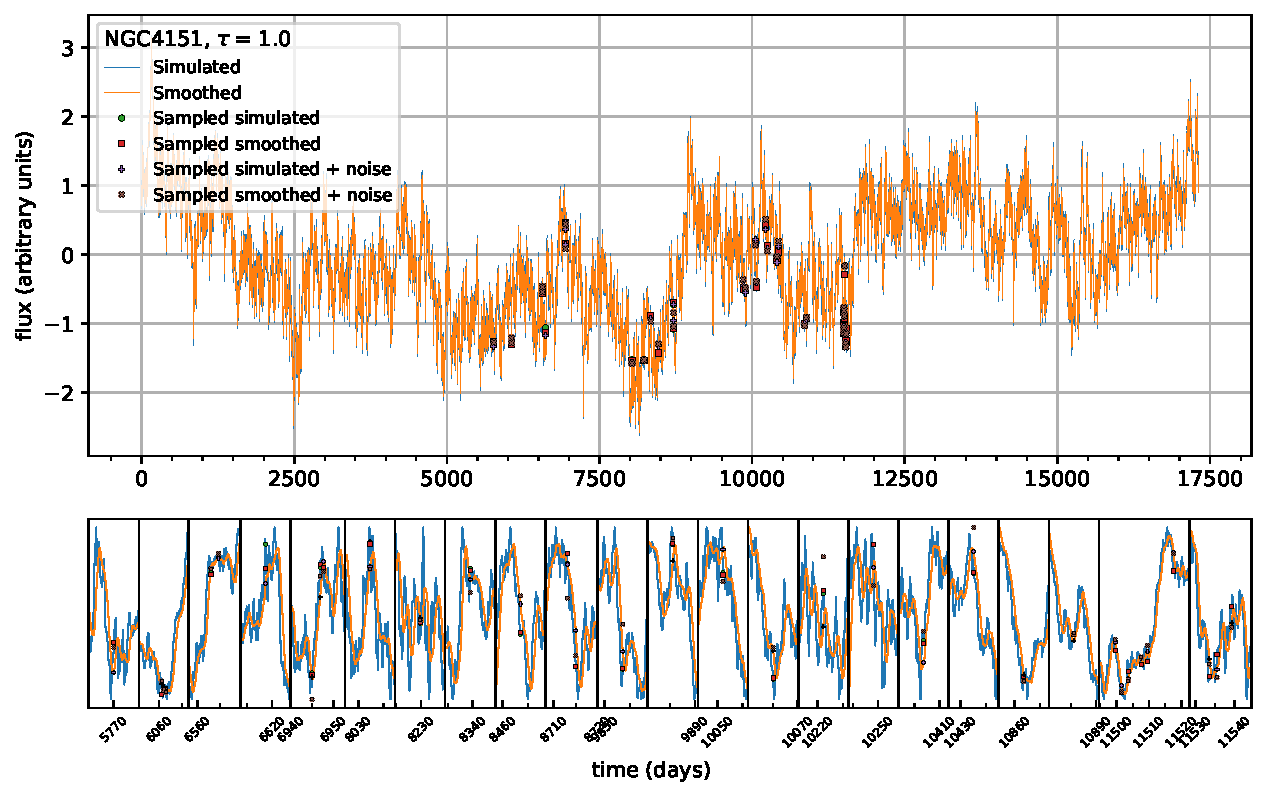
\includegraphics[width=0.49\textwidth]{Figs/Chapter5/NGC4151/sim_LC_tau1.0_0_matrix.pdf} \\
  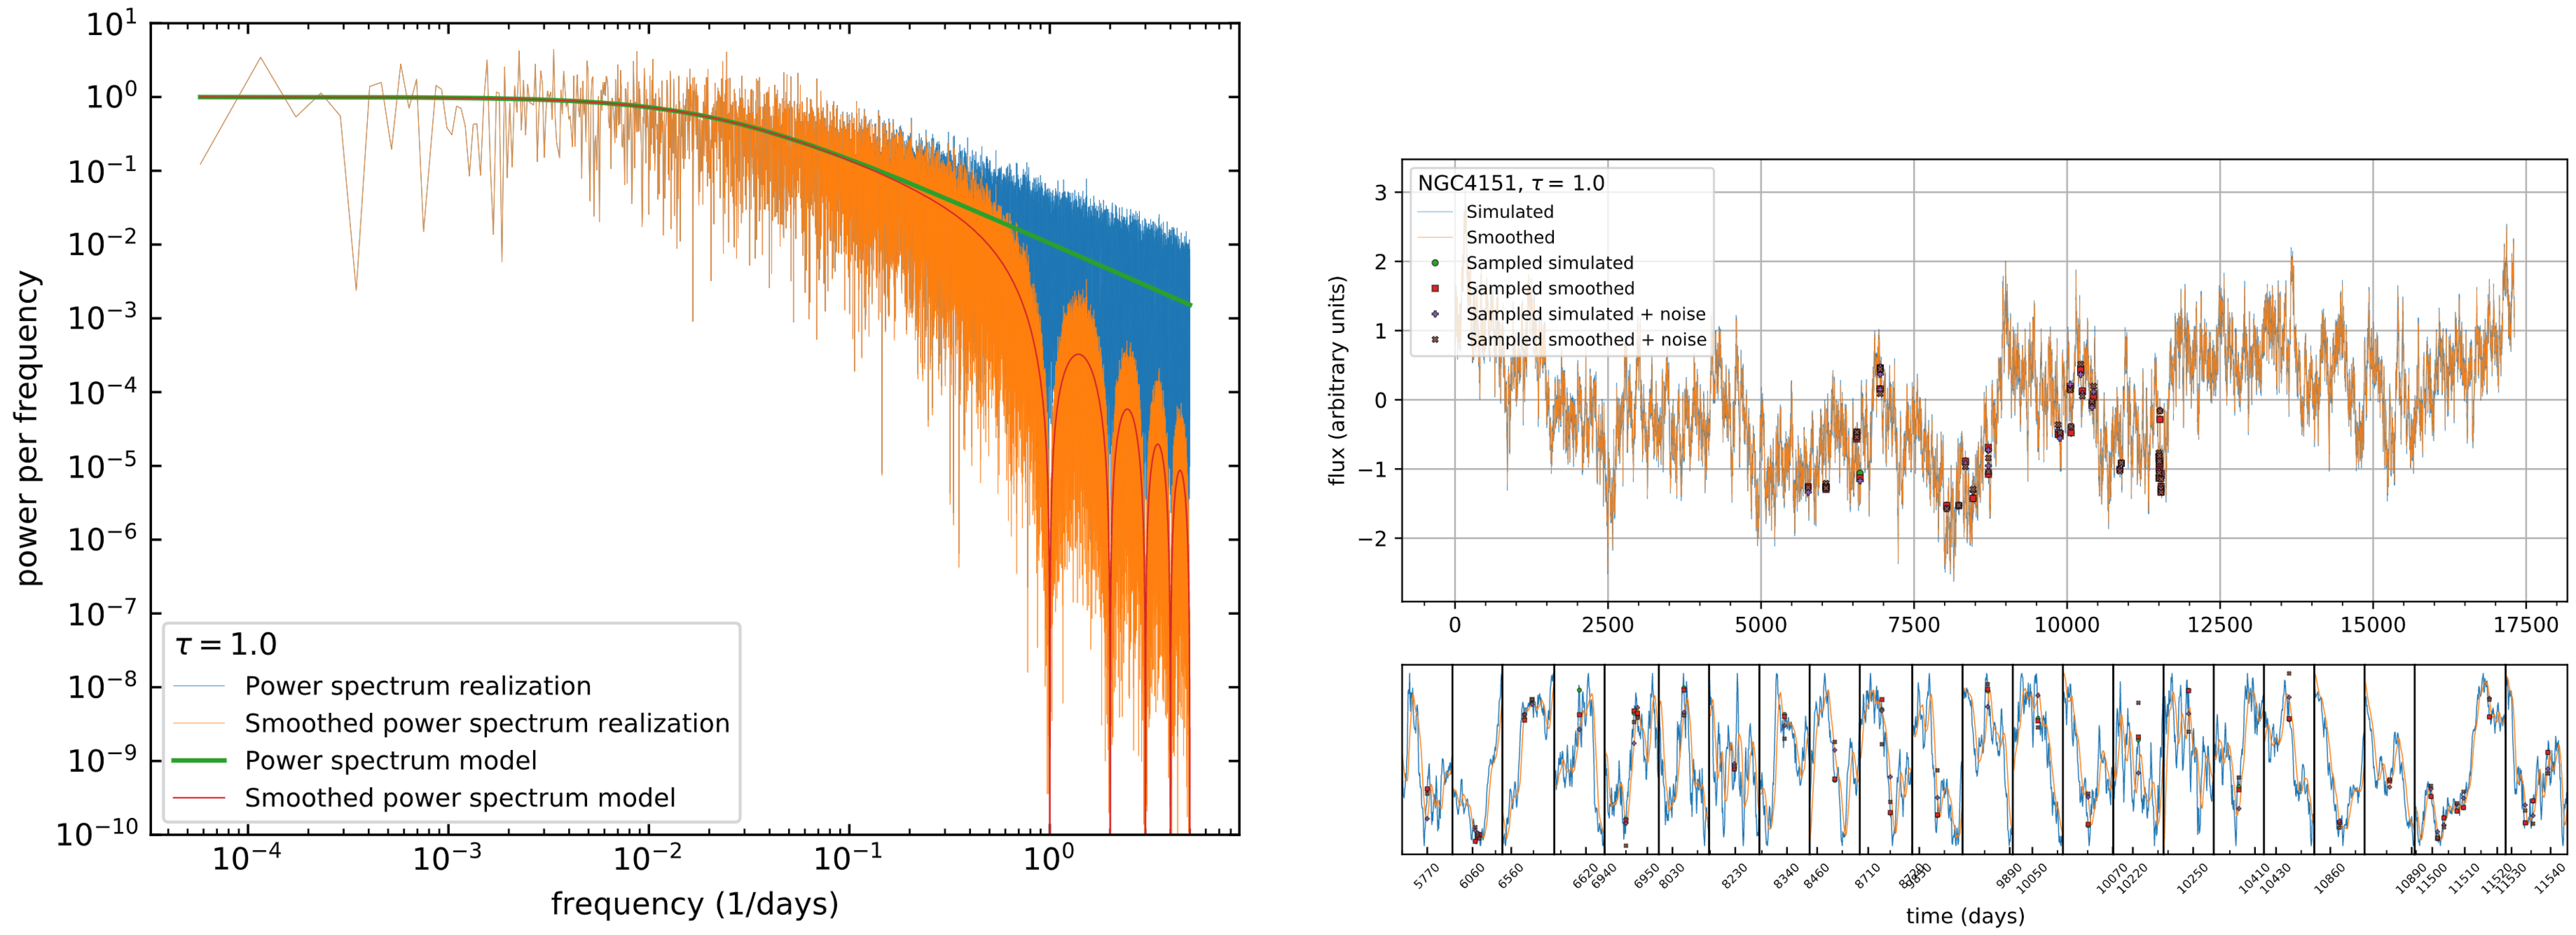
\includegraphics[width=\textwidth]{Figs/Chapter5/NGC4151/Screenshots/NGC4151_tau1_LC_spectrum.pdf} \\
 % 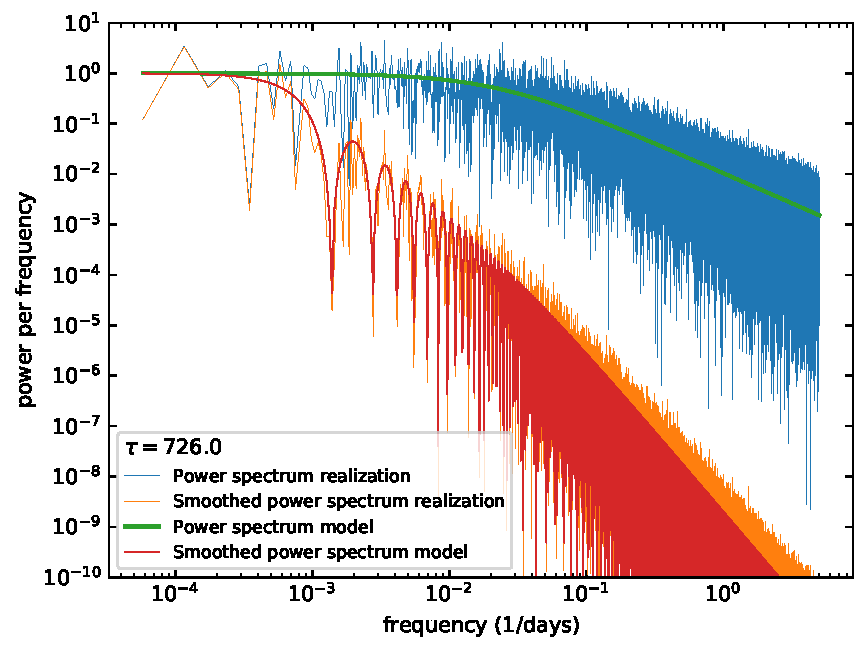
\includegraphics[width=0.49\textwidth]{Figs/Chapter5/NGC4151/power_spectrum_tau726.0.pdf}\hfill 
 % 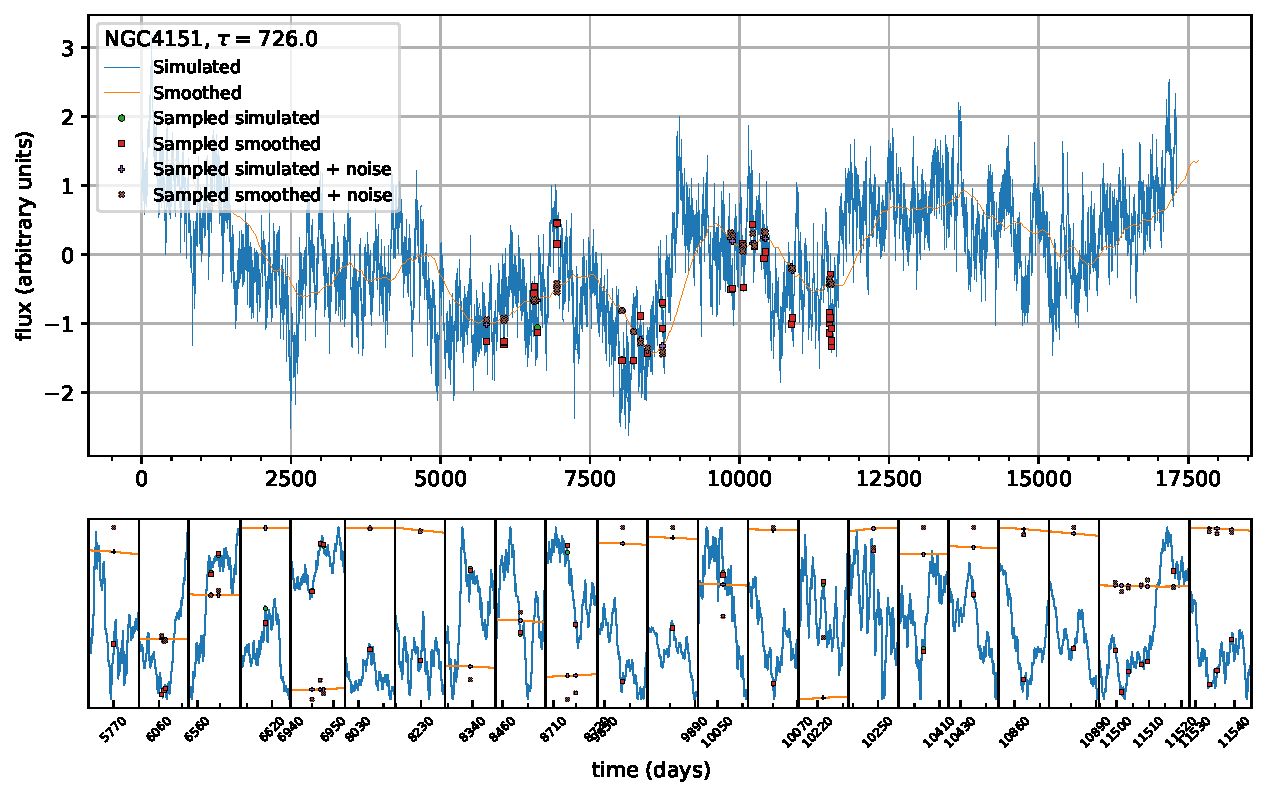
\includegraphics[width=0.49\textwidth]{Figs/Chapter5/NGC4151/sim_LC_tau726.0_0_matrix.pdf} \\
  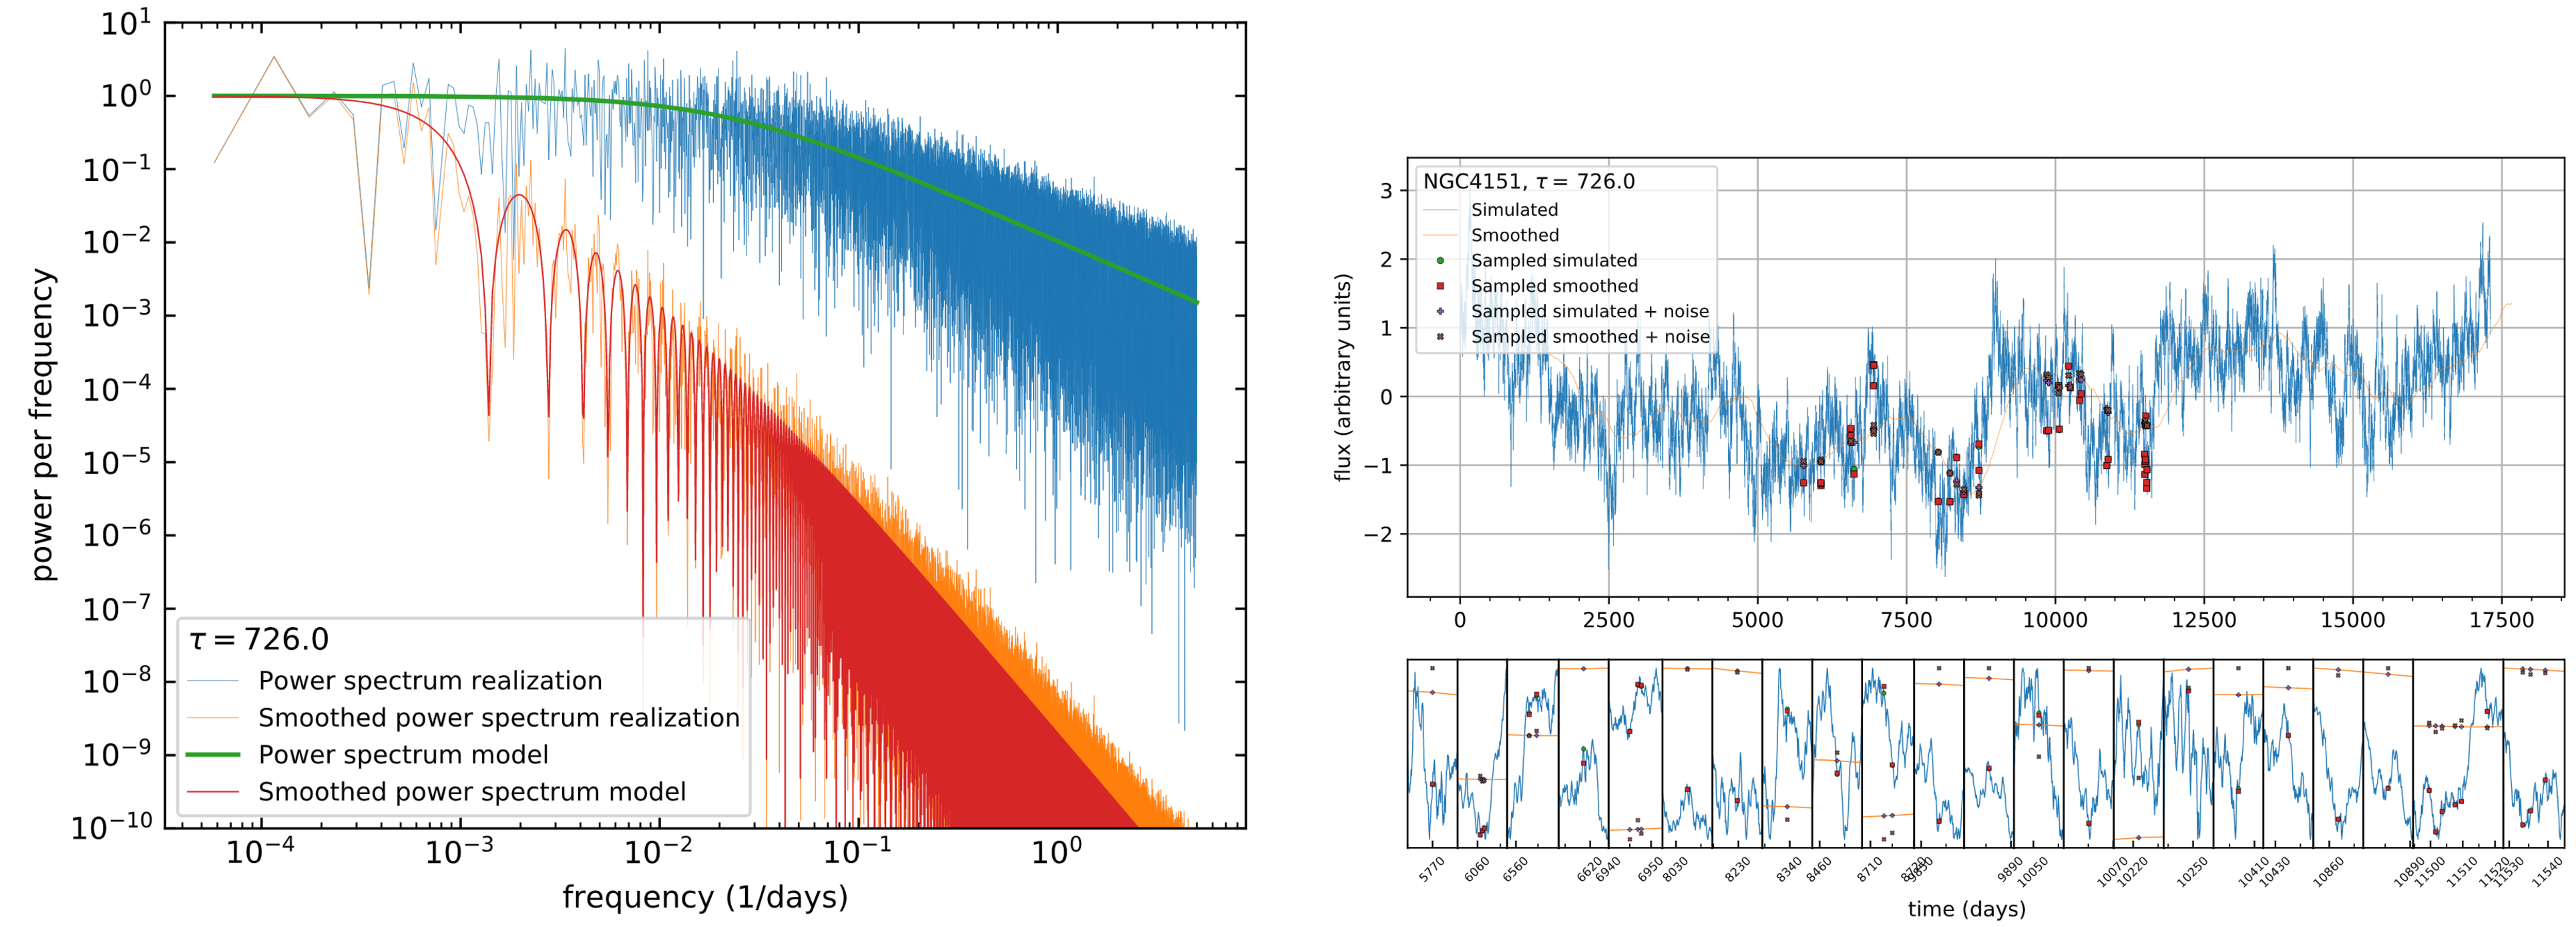
\includegraphics[width=\textwidth]{Figs/Chapter5/NGC4151/Screenshots/NGC4151_tau726_LC_spectrum.pdf} \\
%  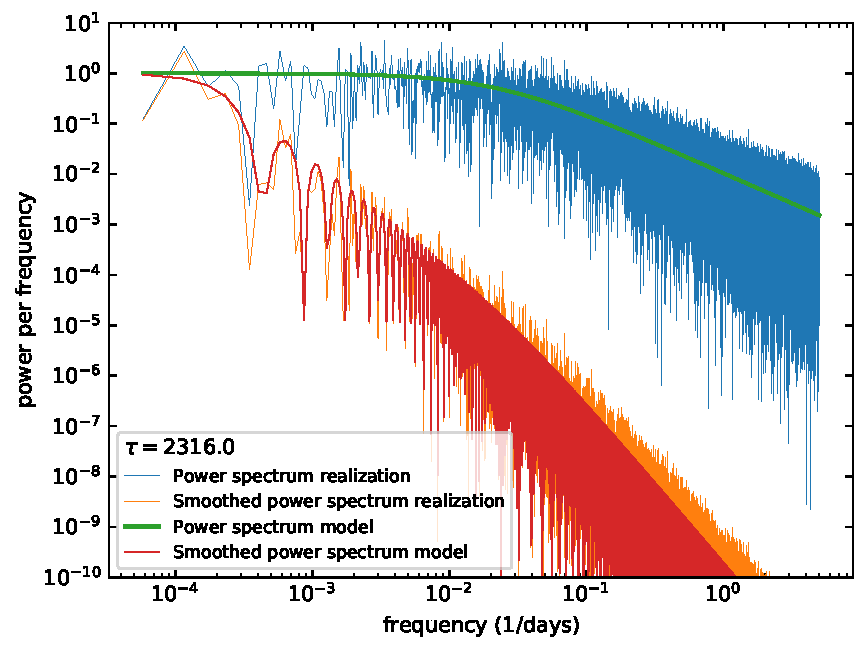
\includegraphics[width=0.49\textwidth]{Figs/Chapter5/NGC4151/power_spectrum_tau2316.0.pdf} \hfill 
%  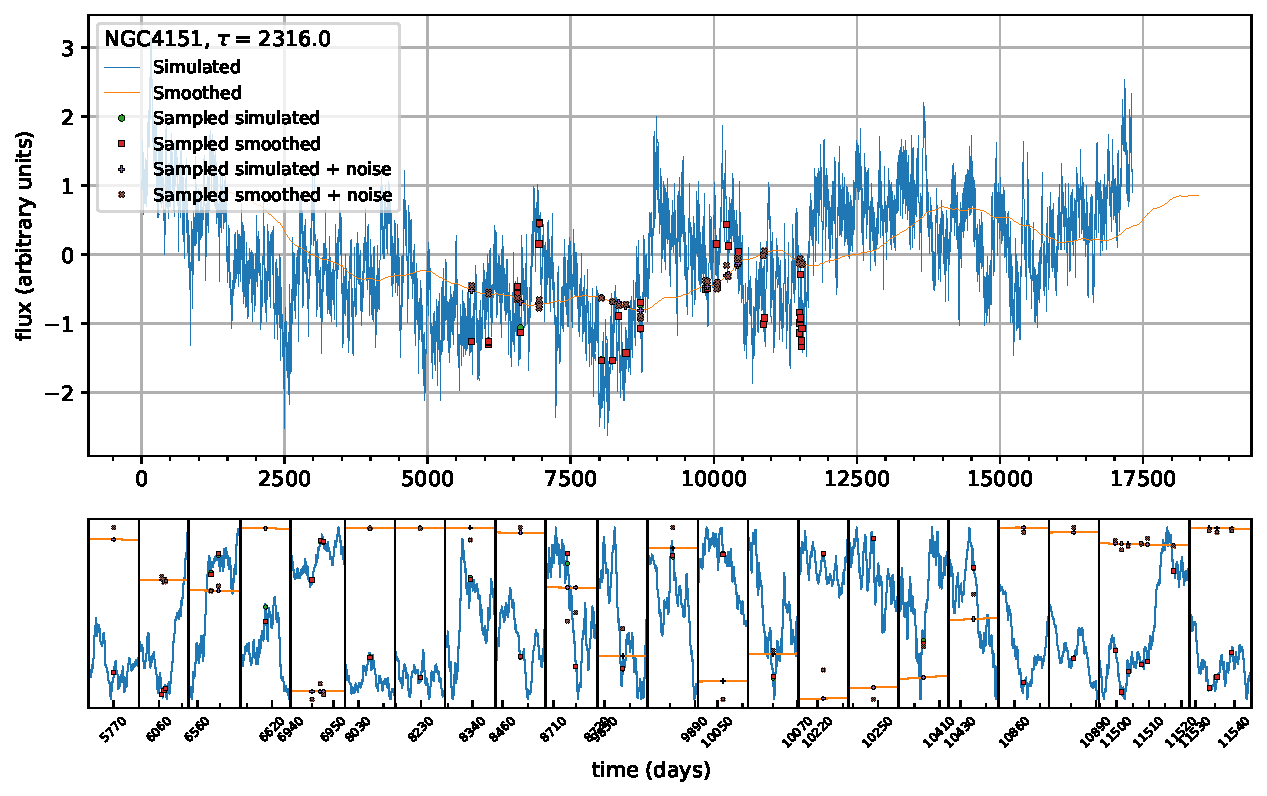
\includegraphics[width=0.49\textwidth]{Figs/Chapter5/NGC4151/sim_LC_tau2316.0_0_matrix.pdf} \\
  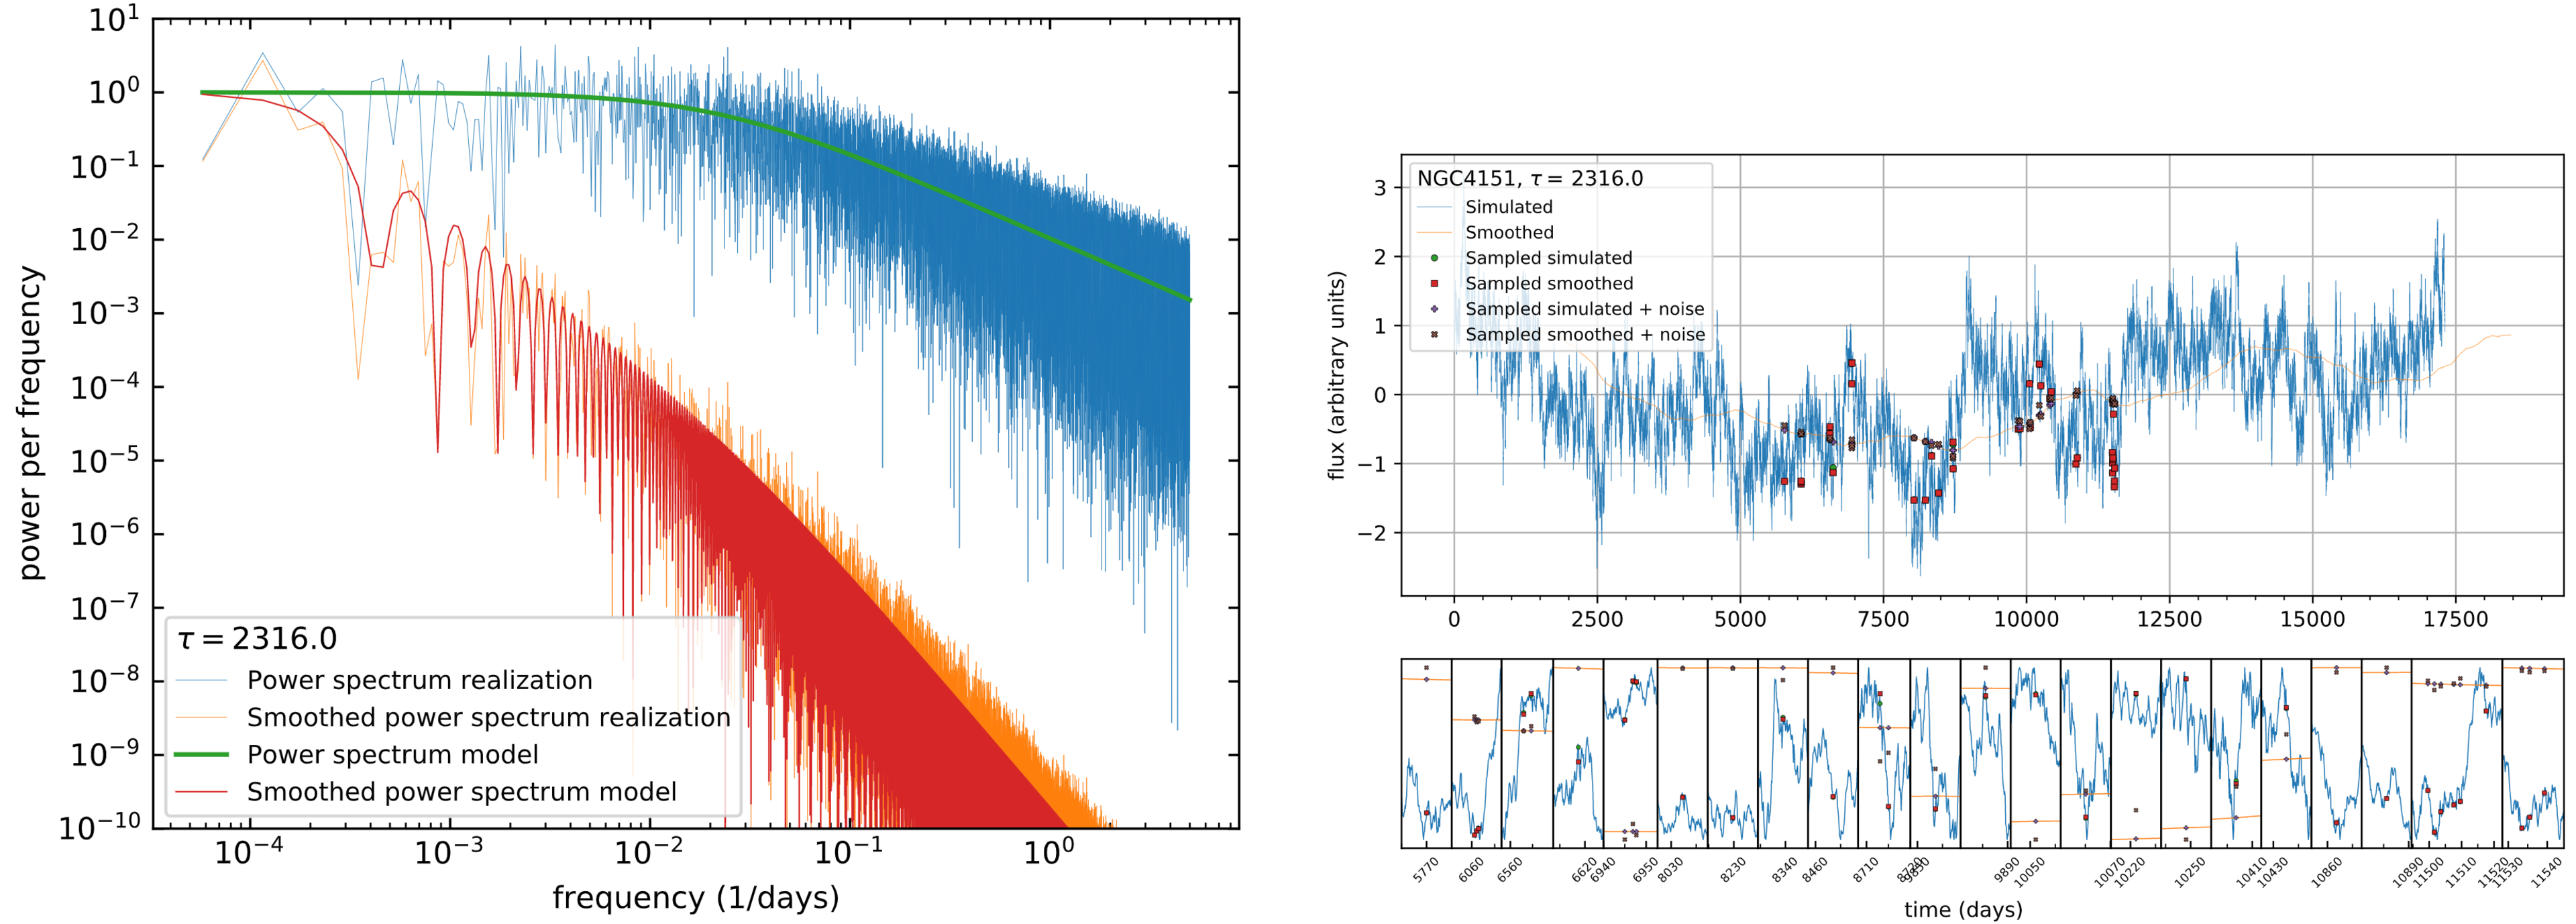
\includegraphics[width=\textwidth]{Figs/Chapter5/NGC4151/Screenshots/NGC4151_tau2316_LC_spectrum.pdf} \\
  \caption{Power spectrum NGC4151}
    \label{fig:power_spectra_1_NGC4151}
  }
\end{center}
\end{figure}

\begin{figure}
\begin{center}
    {
  %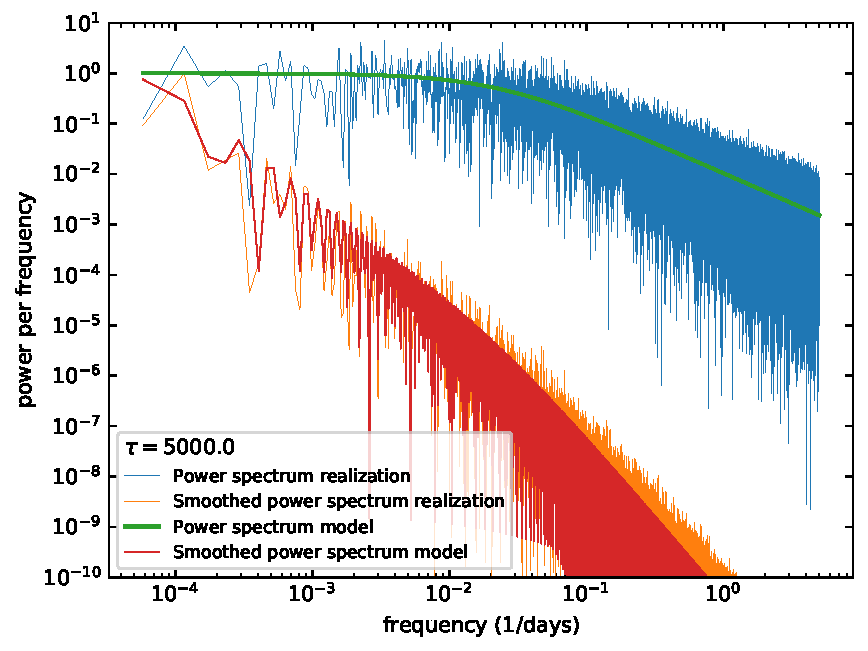
\includegraphics[width=0.49\textwidth]{Figs/Chapter5/NGC4151/power_spectrum_tau5000.0.pdf} \hfill 
  %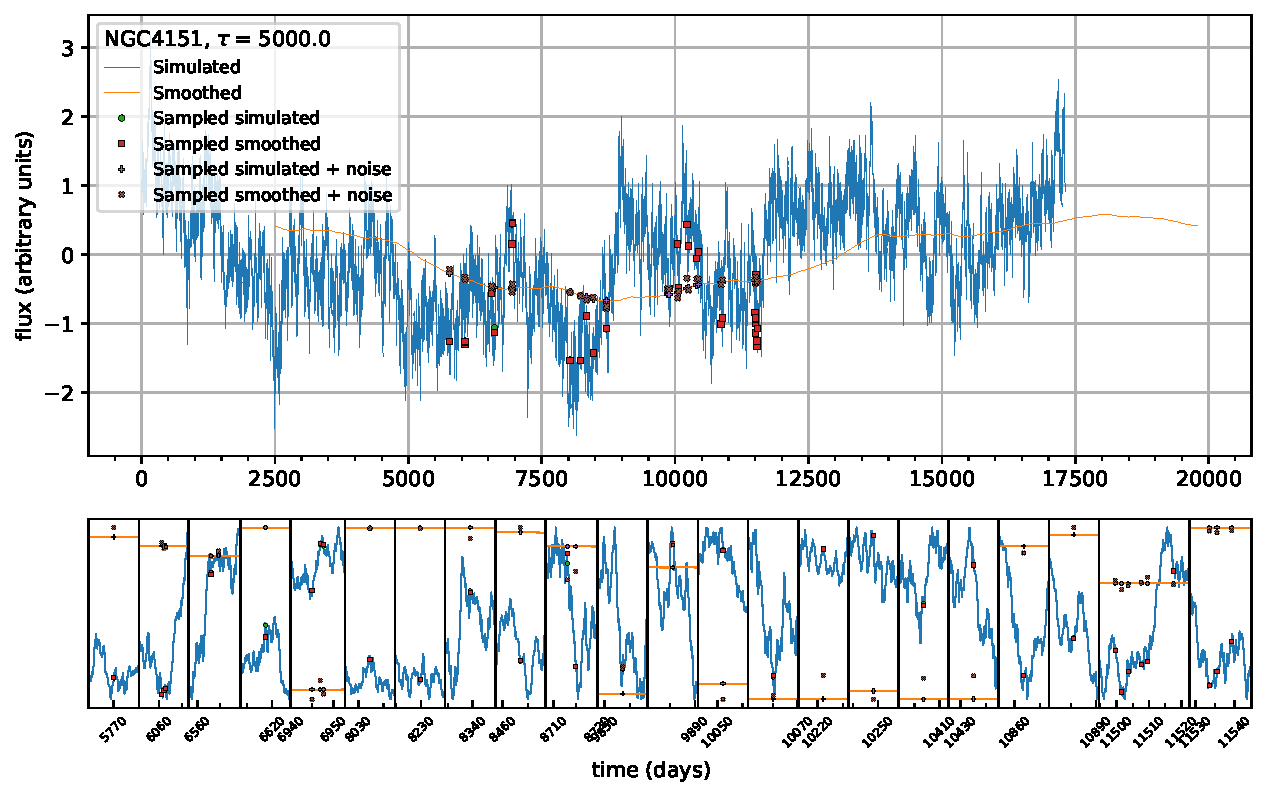
\includegraphics[width=0.49\textwidth]{Figs/Chapter5/NGC4151/sim_LC_tau5000.0_0_matrix.pdf} \\
  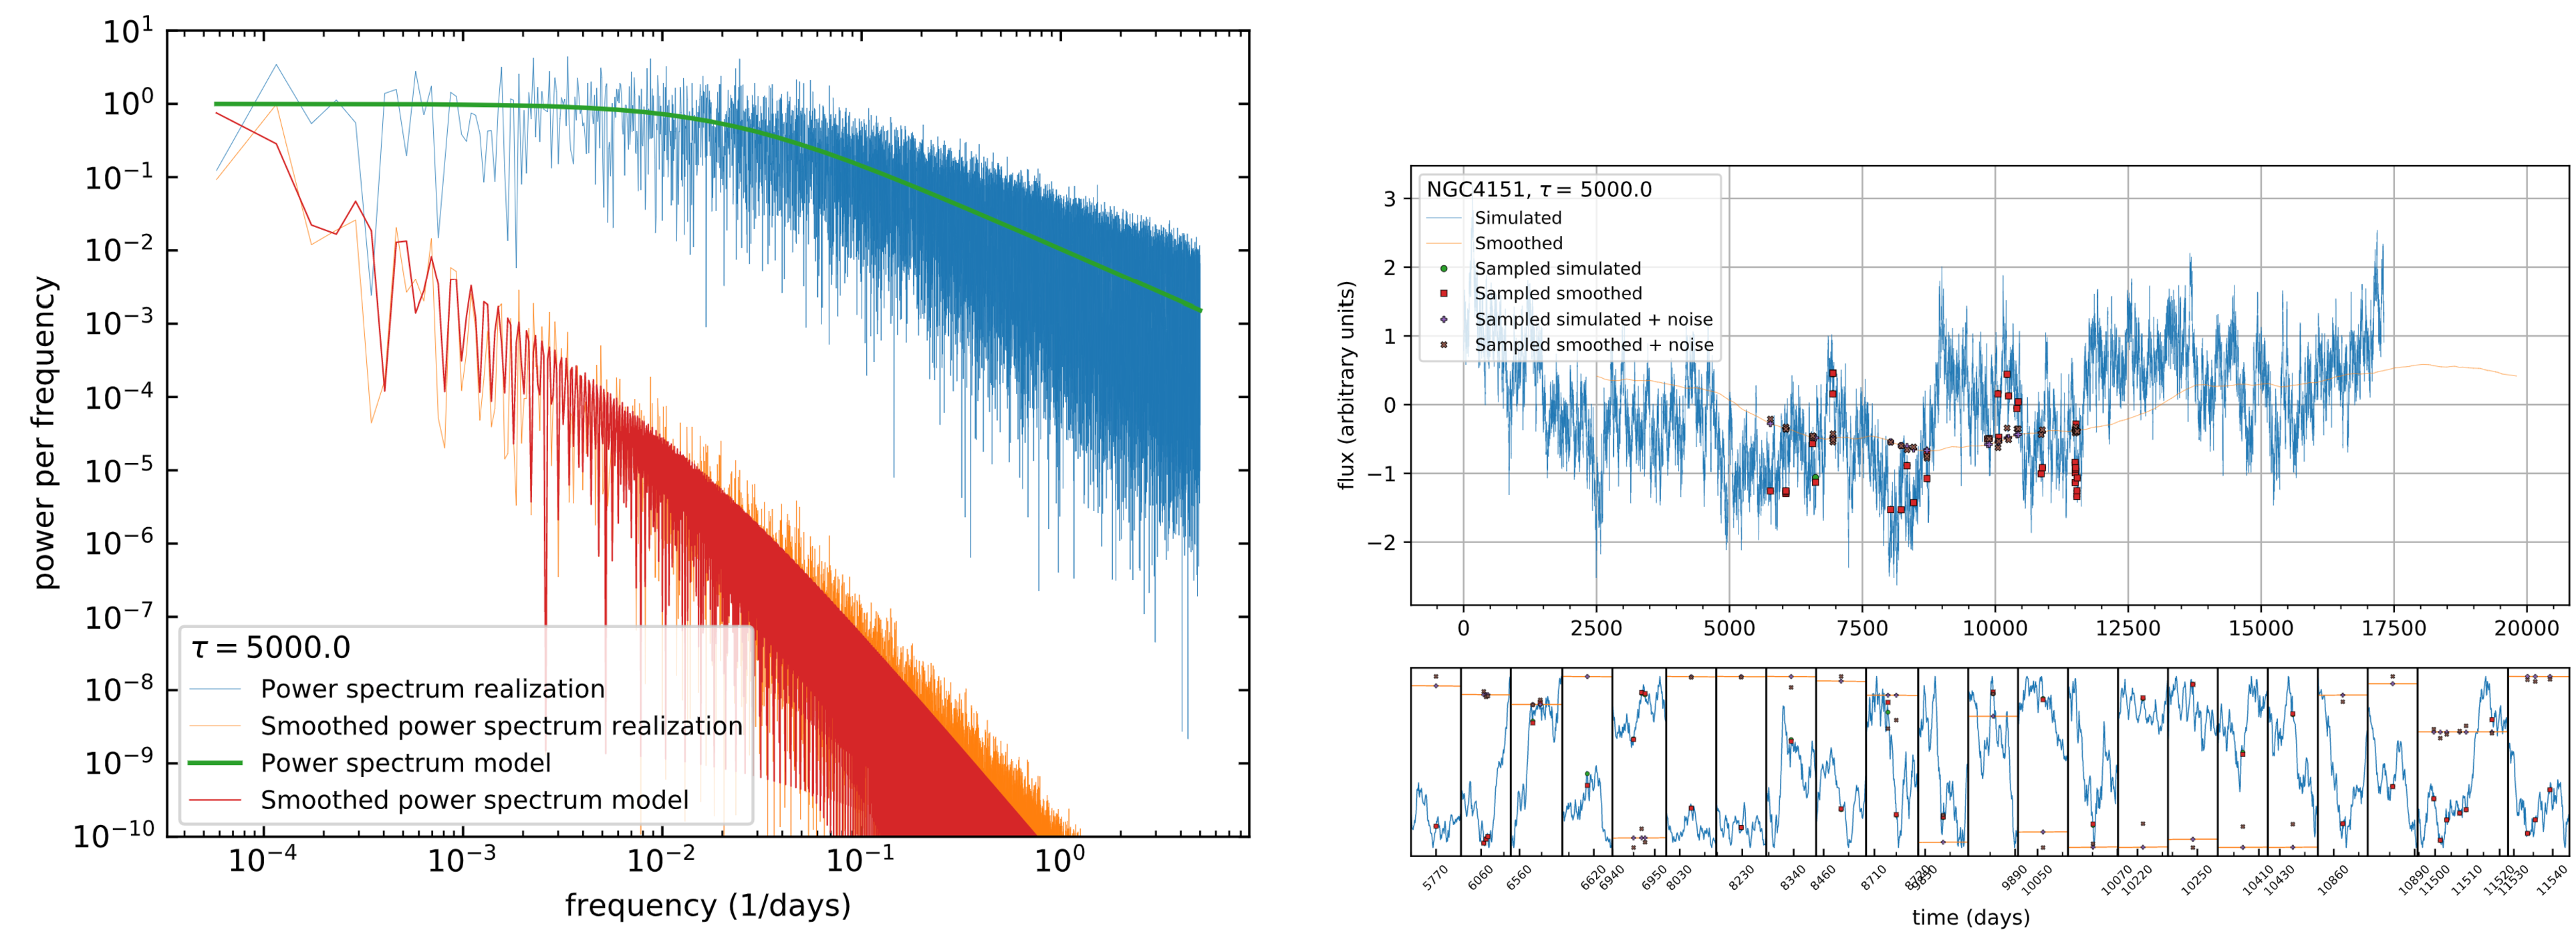
\includegraphics[width=\textwidth]{Figs/Chapter5/NGC4151/Screenshots/NGC4151_tau5000_LC_spectrum.pdf} \\
  %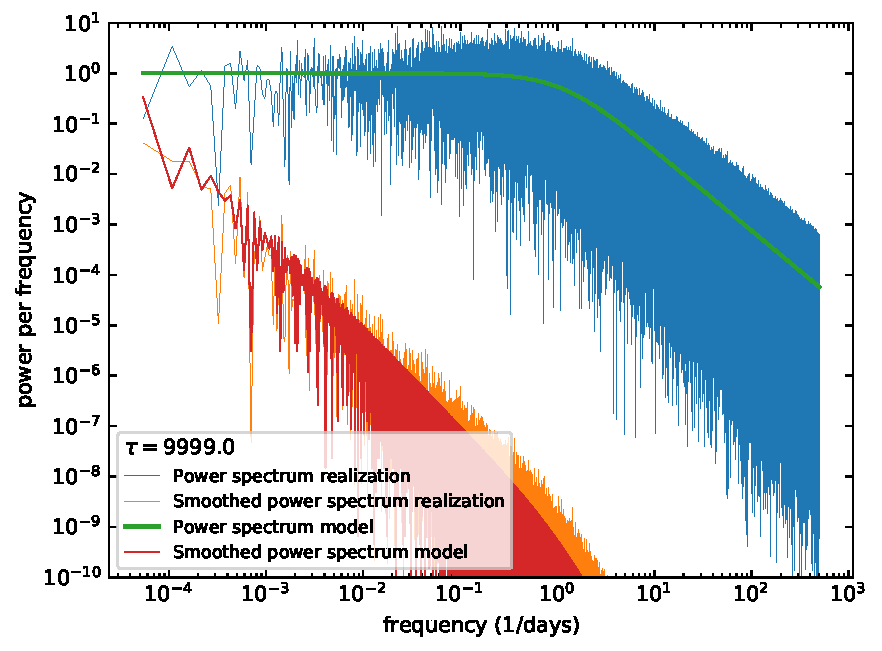
\includegraphics[width=0.49\textwidth]{Figs/Chapter5/NGC4151/power_spectrum_tau9999.0.pdf} \hfill 
  %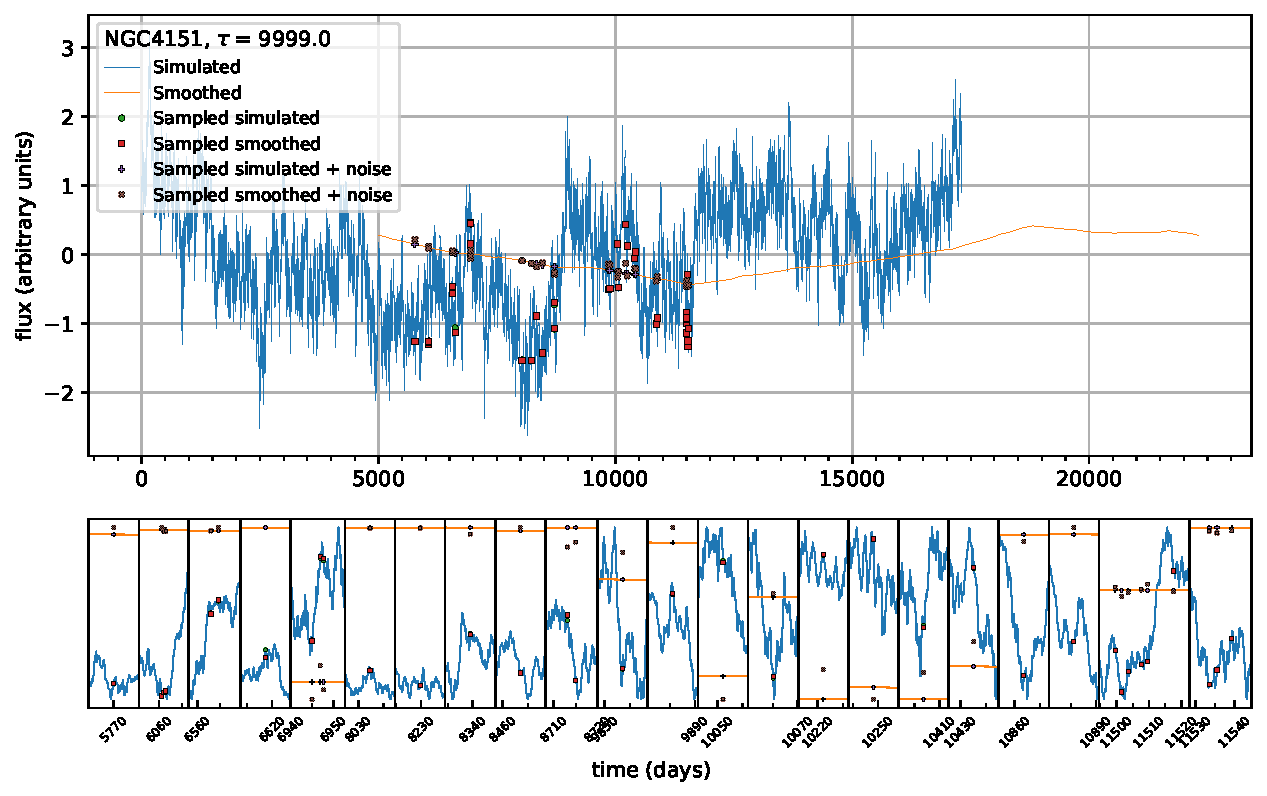
\includegraphics[width=0.49\textwidth]{Figs/Chapter5/NGC4151/sim_LC_tau9999.0_0_matrix.pdf} \\
  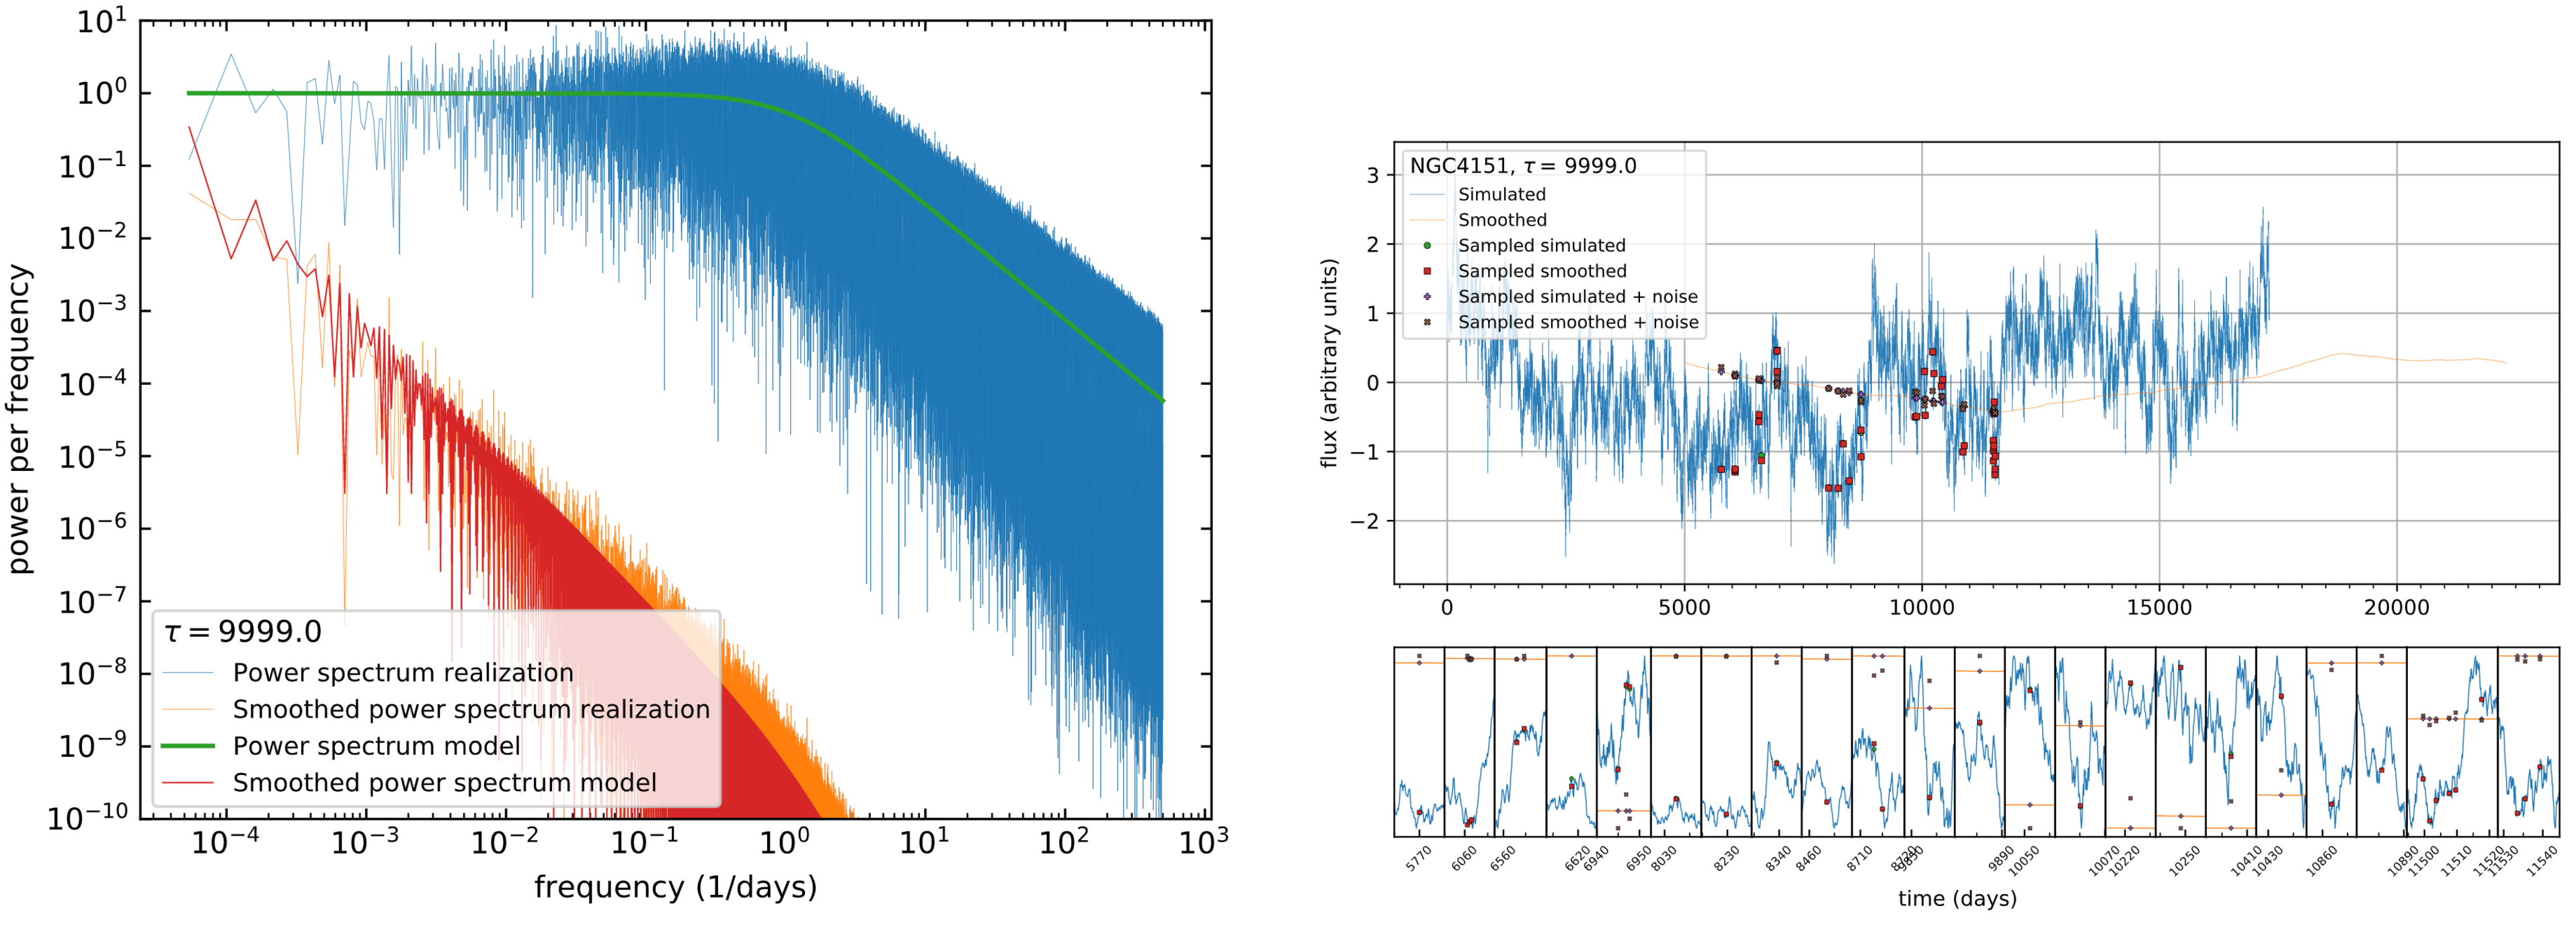
\includegraphics[width=\textwidth]{Figs/Chapter5/NGC4151/Screenshots/NGC4151_tau9999_LC_spectrum.pdf} \\
  \caption{Power spectrum NGC4151}
    \label{fig:power_spectra_2_NGC4151}
  }
\end{center}
\end{figure}

For each source we consider its spectral parameters and in particular we choose a sampling time-scale $dt$ based on its bending time-scale as $dt=10^{{\rm floor}(\log_{10}(T_b/100)}$, i.e. the sampling resolution is at least a 100th of the $T_b$ scale and is an entire number in the representation $\log(dt)$. This choice results in values $-4\le\log(dt)\le-1$. We resampled the simulated light curves according to the observed epochs and added Gaussian noise to each simulated data-point with a standard deviation scaled based on the error of the observation at that epoch, in order to reproduce the additional variance of the data. Finally, we computed the ratio of the variances ($\xi_{\rm r,sim}=\sigma^2_{\rm Fe, sim}/\sigma^2_{\rm c,sim}$). As expected, this ratio decreases as the light crossing time of the reflector increases. We ran sets of 50 simulations and recorded the mean and root-mean-square deviations (rms) of $\xi_{\rm r,sim}$ for a range of values of the light crossing time. We implemented the following statistic to find the $\tau$ values which correspond to our estimated reprocessor size and its upper and lower limits:
\begin{equation}
    {\rm X}(\tau)=\frac{\xi_{\rm data}-<\xi_{\rm sim}>}{(\xi_{\rm sim})_{rms}}
    \label{eq:X_tau}
\end{equation}
 where $\xi_{r,real}$ is the median value of the $\xi_{r}$ distribution. %We solved the equation for $X=0,-1,1$, which correspond to the $\tau$ best fitting value, the upper limit of $\tau$ at $1\sigma$, and lower limit of $\tau$ at $1\sigma$, respectively.  
 
 Examples of the power spectra used to simulate light curves are reported in the left panels of Figs.~\ref{fig:power_spectra_1_NGC3783} and \ref{fig:power_spectra_2_NGC3783} for NGC 3783 and Figs.~\ref{fig:power_spectra_1_NGC4151} and ~\ref{fig:power_spectra_2_NGC4151} for NGC 4151, for both the continuum and \kalfa{} ("smoothed"). These two galaxies were chosen as an example of very different $\nu_b$ frequencies and because we were able to find all three $\tau$ values corresponding to $X=0,1,-1$. In the model power spectrum (green line) we can see a decrease in power after the break frequency, which is $\nu_b=1.1 \,{\rm days}^{-1}$ for NGC 3783 and $\nu_b=0.022\,{\rm days}^{-1}$ for NGC 4151. We also see a decrease in the smoothed power spectrum (red line) at frequencies higher that $1/\tau$, where $\tau$ is shown in the legend title of each figure and is shown in increasing order.
 
    In the right panels of the aforementioned Figures we show the light curves associated with the power spectra on the left, and we also show the resampled data points from the light curves. The blue light curve corresponds to the realization of the power spectrum in blue as well in the left panel, and the orange light curve is the smoothed curve which corresponds to the smoothed power spectrum realization, in orange as well. It can be seen that a higher $\tau$ corresponds to a higher smoothing in the light curve, as expected, and a non obvious correlation between the two light curves, especially with such poor sampling. This can be better seen in the lower panels on the right, which are a zoom in in correspondence to the observed data points, but especially in Fig.~\ref{fig:Flux-flux_NGC3783} and ~\ref{fig:Flux-flux_NGC4151}, which show flux-flux plots for some $\tau$ values. 
 
The $\tau*$ values that return $X=0,1,-1$ correspond to the reprocessor size in light days and its upper and lower limits at $\pm1\sigma$, respectively. In order to constrain the size of the reprocessor, we first explore a range of $\tau$ values between 1-10,000 days, and then numerically look for the roots $X=0,1,-1$ using Newton's method. The resulting $X(\tau)$ relations explored for each source are shown in Appendix~\ref{appendix_lightcurves} while the reprocessor sizes thus determined are discussed in Section~\ref{sec:lc_results}.

\section{Correlation between Fe line and continuum flux} \label{sec:lc_results}

A strong, positive correlation between these two fluxes, which is much simpler to assess compared to more complicated lag analyses, should indicate that the reflector lies in close proximity to the source of the X-ray continuum emission. 
Thus we explore potential correlations between the observed 2--10 keV continuum and Fe $\rm K\alpha$ line light curves for sources in our sample. As mentioned above, any lag in the \kalfa{} line light curves, which is expected from reprocessing travel time delays, can reduce the apparent correlation between the observed light curves. The degree of loss of correlation is a function of the ratio between the light crossing time of the reprocessor and the characteristic timescales of fluctuations, as well as the geometry of the reprocessor. 

The green data-points and the relative green best fit in Figs.~\ref{fig:Flux-flux_NGC3783},~\ref{fig:Flux-flux_NGC4151} show one realization of the resampled continuum and reprocessed (\kalfa{}) light curves corresponding to our best estimate of the reprocessor size $\tau*$ while in orange and red we show the resampled data points and best fit our our upper and lower limit (one realization). These relations don't necessarily show a correlation between the observed (data, shown with brown crosses) and simulated light curves, but this is due to the delay and the sampling of the data, as we've shown in the previous paragraph, and it doesn't imply that they aren't correlated.

To better show this we refer the reader to Figs.~\ref{fig:Flux-flux_all_1},~\ref{fig:Flux-flux_all_2}~\ref{fig:Flux-flux_all_3}~\ref{fig:Flux-flux_all_4},~\ref{fig:Flux-flux_all_5}, where for each source in our sample for which we were able to determine $\tau*$ such that $X(\tau*)=0$, we show all the best fits of the flux-flux relations of the 50 simulated light curves, versus the data and their best fit. We also show in the right panels a histogram of the slopes of the linear fits of the simulations versus the slope of the observed data. We can see that in many cases the slope of the data is compatible with the range of the slopes from the simulated light curves.

We show in Table~\ref{tab:taus} the $\tau*$ values of each source sorted by the median $\xi$. As already mentioned in Section~\ref{sec:variability_defs}, per definition in Eq.~\ref{eq:xi}, the $\xi$ will be $\approx 1$ if the reprocessor is nuclear, i.e.  very small, and $\xi\gtrsim 0$ if the reprocessor is extended. 
There are also two cases in which the size of the reprocessor cannot be constrained, these are $\xi<0$ when the uncertainty on the data is greater than their variation, and $\xi>1$ if the variance of the \kalfa{} line is greater than that of the continuum. 
The first case, $\xi<0$, occurs when the uncertainty on the data is greater than their variation and this happens to be the case for the \kalfa{} light curve of the affected sources. However, the upper limit on the ratio of excess variance of these sources is still $>0$, therefore it could also be a matter of overestimation of the noise because of the error on the noise (Eq.~\ref{eq:NXS_err}).
In the latter case, $\xi>1$, either the poor sampling of the light cures did not seize the wider variations of the continuum, or the \kalfa{} line may not be reflecting the variations of the continuum and therefore the reprocessor cannot be modeled in our physical description of the AGN as introduced in Sec.~\ref{sec:LC_sims}. A physical example of this situation could be a radio loud source where a cloud reflects towards us the beamed X-ray emission associated with the powerful jets, leading to stronger and/or more rapid variations in the \kalfa{} line than in the continuum.
We see in Table~\ref{tab:taus} that we were not able to constrain the $\tau*$ values when $\xi<0$ and $\xi>1$. Instead, in the intermediate cases we were able to place some constraints, especially when both the upper and lower limits of $\xi$ are well constrained in the range (0,1), like in the cases of NGC 2992, NGC 7582, NGC 4388, NGC 1365, NGC 4151, NGC 3783, MRK 1040. When $\xi$ and its lower limit were very low and/or compatible with negative, meaning that the reprocessor is very extended (and/or data quality is bad?), we were able to determine a lower limit on the size of the reprocessor. On the contrary, when $\xi$ and its upper limit were close to one, meaning that the reprocessor is small (and/or bad signal to noise in continuum data?), we were able to place an upper limit on the size of the reprocessor. Roughly $\approx$22\% (9/41) lie above 1, although all are consistent with unity (red line in Fig.~\ref{fig:exvars}) to within 2-$\sigma$ uncertainties. In total, more than 50\% have values consistent with unity, implying little damping of the continuum by the reflector (i.e., angle-averaged light-crossing timescales to the reflector comparable to the continuum variability timescales), or alternatively that we are not observing the true continuum fluctuations. Sometimes, when the $\xi$ value was not well constrained and outside of the (0,1) range we were able to determine the size of the reprocessor, but not its $1\sigma$ limits, or maybe we weren't able to determine any constraint. The complete range of $X(\tau)$ determined for each source is shown in Appendix~\ref{appendix_lightcurves}.

We were able to completely constrain the size of the reprocessor, i.e. best value size and $1\sigma$ uncertainties, for a total of 4 sources and at least one of the limits for 13 sources. For the remaining 16 sources we weren't able to constrain the reprocessor size. This is still a remarkable result, given the sparsity of our light curves and the inconsistent quality of the archival data. Furthermore, the physical model we adopt is extremely simple and may not properly describe all of the source. In fact, more realistic distributions could be thicker, clumpier, and have a toroidal or ionization cone-like structure seen at a specific orientation with respect to the line-of-sight, all of which can impact delay times and smoothing. (argumentar mas?)

\begin{longtable}{llrrr}
%\caption{lallero}
\label{tab:taus}\\
\toprule
{} & $\xi(50\%)_{16\%}^{84\%}$   & $\tau_{inf}$ & $\tau_{best}$ & $\tau_{sup}$ \\
{} &                           & (light days) &  (light days) & (light days) \\
\midrule
\endhead
\midrule
\multicolumn{5}{r}{{Continued on next page}} \\
\midrule
\endfoot

%\bottomrule
\endlastfoot
3C120                  &      $ -1.3_{-19.}^{6.6} $ &       - &        - &       - \\
CygnusA                &     $ -0.51_{-6.0}^{3.7} $ &       - &        - &       - \\
PictorA                &    $ -0.34_{-3.1}^{0.88} $ &       - &        - &       - \\
1H0707-495             &   $ -0.18_{-0.82}^{0.28} $ &       1 &        - &       - \\
NGC7469                &   $ -0.036_{-1.2}^{0.68} $ &       - &        - &       - \\
NGC2992                &  $ 0.031_{0.019}^{0.040} $ &     377 &     9713 &       - \\
NGC5548                &  $ 0.042_{-0.071}^{0.15} $ &      99 &        - &       - \\
NGC7582                &  $ 0.070_{0.018}^{0.094} $ &     200 &     8548 &       - \\
MRK766                 &    $ 0.11_{-0.35}^{0.43} $ &       - &       18 &       - \\
MRK290                 &      $ 0.13_{-1.7}^{1.4} $ &       - &      231 &       - \\
2MASXJ11315154-1231587 &   $ 0.20_{-0.026}^{0.39} $ &     112 &     3168 &       - \\
NGC4388                &     $ 0.20_{0.13}^{0.26} $ &       2 &     3013 &    6602 \\
NGC1365                &     $ 0.22_{0.19}^{0.25} $ &      45 &     1999 &    4652 \\
NGC4151                &     $ 0.24_{0.22}^{0.25} $ &     726 &     2316 &    5000 \\
NGC3393                &      $ 0.29_{-1.7}^{1.7} $ &       - &        - &       - \\
MRK273                 &     $ 0.43_{-0.90}^{1.0} $ &       - &     1364 &    5703 \\
NGC3783                &     $ 0.45_{0.29}^{0.58} $ &       6 &      271 &    1675 \\
MRK1040                &     $ 0.57_{0.18}^{0.82} $ &       - &       14 &     903 \\
MRK3                   &      $ 0.73_{0.12}^{1.3} $ &       - &        - &       3 \\
MRK509                 &     $ 0.76_{-0.81}^{1.8} $ &       - &       84 &    2418 \\
NGC1275                &     $ 0.82_{0.025}^{1.3} $ &       - &       15 &       - \\
CenA                   &      $ 0.92_{0.66}^{1.1} $ &       - &        - &      51 \\
IC4329A                &      $ 0.99_{0.47}^{1.3} $ &       - &        1 &     385 \\
NGC3516                &      $ 1.0_{-0.68}^{2.0} $ &       - &        - &    1988 \\
CircinusGalaxy         &       $ 1.1_{0.33}^{1.8} $ &       - &        - &       5 \\
NGC4051                &       $ 1.8_{-3.3}^{4.4} $ &       - &        - &       - \\
NGC1068                &        $ 2.3_{1.4}^{2.8} $ &       - &        - &       - \\
MCG-6-30-15            &        $ 3.0_{1.5}^{4.2} $ &       - &        - &       - \\
MRK1210                &       $ 3.4_{0.90}^{6.1} $ &       - &        - &       - \\
4C+29.30               &       $ 3.8_{-27.}^{40.} $ &       - &        - &       - \\
MR2251-178             &        $ 5.3_{2.0}^{7.9} $ &       - &        - &       - \\
4C+74.26               &        $ 7.7_{2.1}^{11.} $ &       - &        - &       - \\
3C273                  &       $ 18._{-17.}^{36.} $ &       - &        - &       - \\
\hline
\caption{For each galaxy we show the $\tau*$ such that $X(\tau_{inf})=-1$, $X(\tau_{best})=-1$, and $X(\tau_{sup})=-1$. We also report the $\xi$ values previously shown in Table \ref{tab:gals_obs_par}, and we order the Table based on this column for clarity reasons.}\\
\end{longtable}

\begin{figure}
\begin{center}
    {
  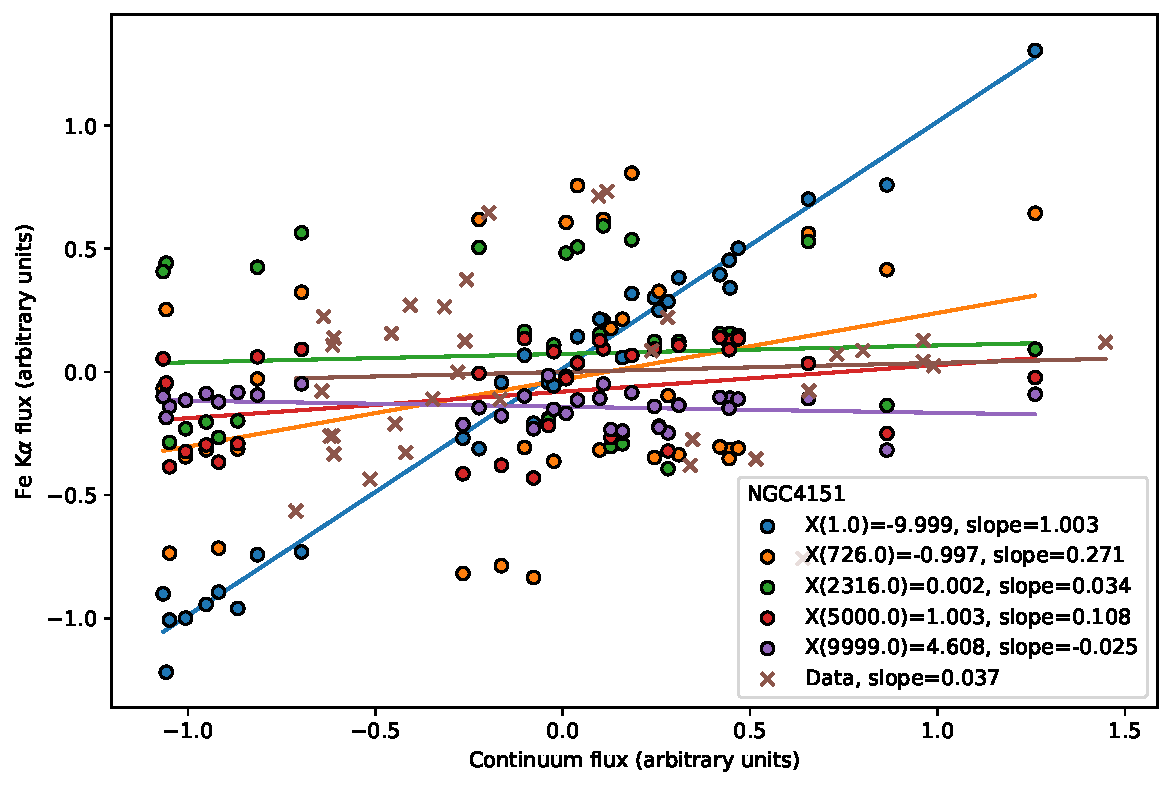
\includegraphics[width=0.7\textwidth]{Figs/Chapter5/NGC4151/Flux_flux_NGC4151.pdf} \hfill 
  \caption{Flux - flux plot NGC4151}
    \label{fig:Flux-flux_NGC4151}
  }
\end{center}
\end{figure}

\begin{figure}
\begin{center}
    {
 % \includegraphics[width=0.49\textwidth]{Figs/Chapter5/NGC3783/power_spectrum_tau1.0.pdf}  \hfill
 % 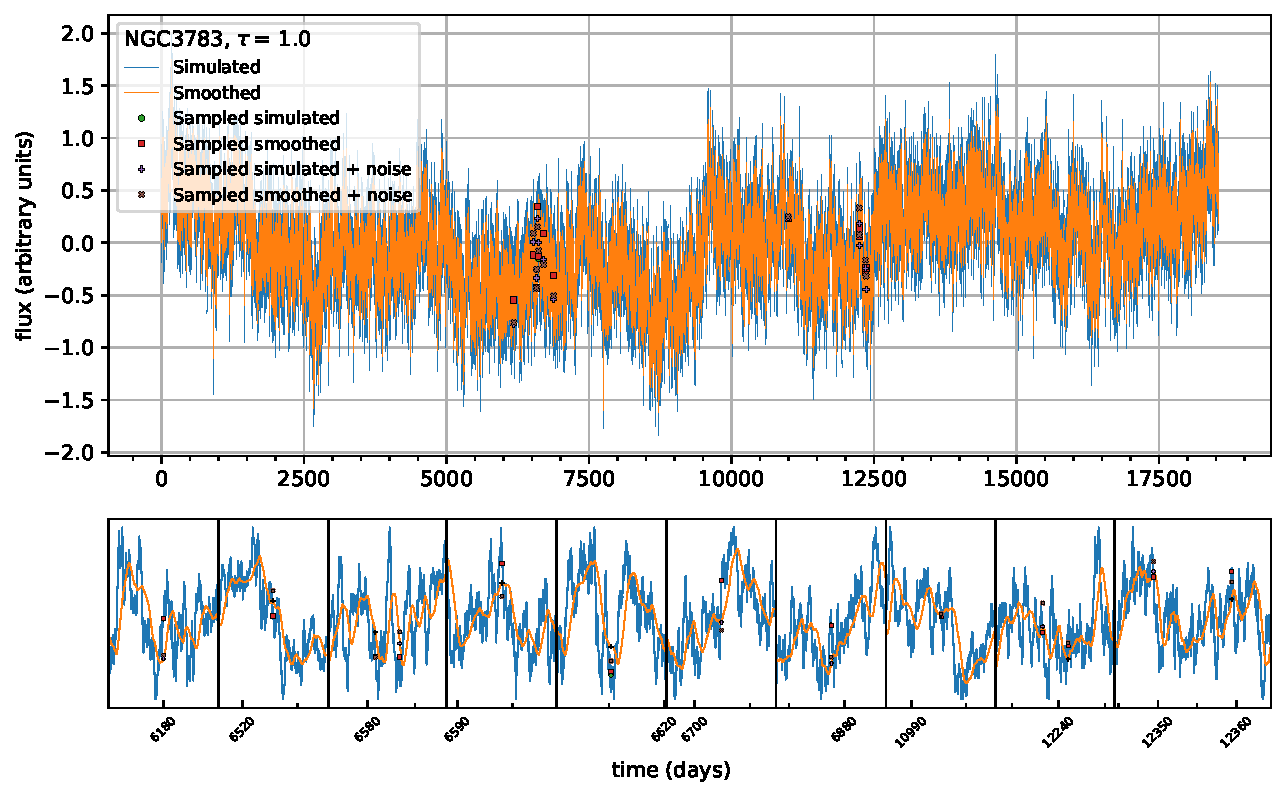
\includegraphics[width=0.49\textwidth]{Figs/Chapter5/NGC3783/sim_LC_tau1.0_0_matrix.pdf} \\
  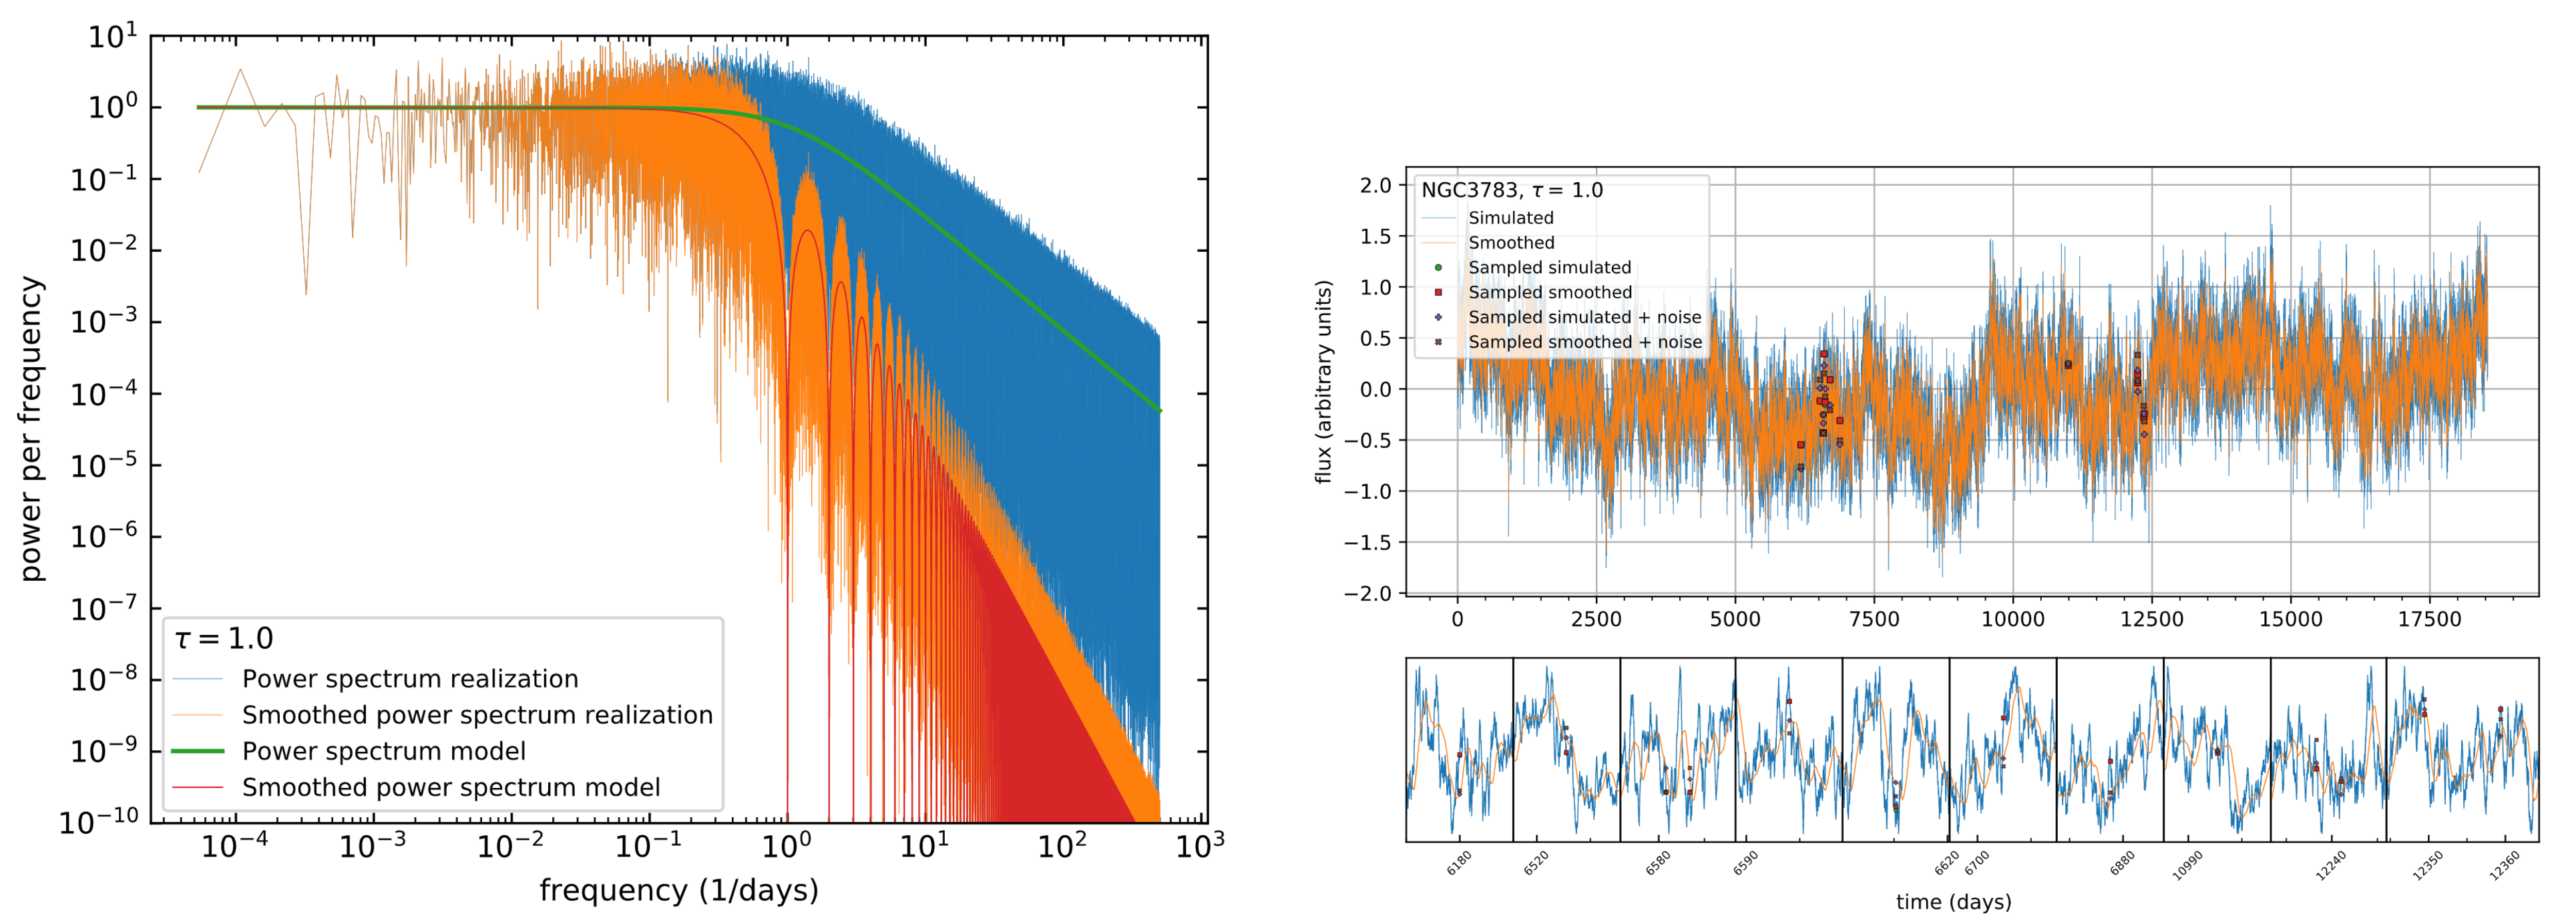
\includegraphics[width=\textwidth]{Figs/Chapter5/NGC3783/Screenshots/NGC3783_tau1_LC_spectrum.pdf} \\
  %\includegraphics[width=0.49\textwidth]{Figs/Chapter5/NGC3783/power_spectrum_tau5.0.pdf}\hfill 
 % 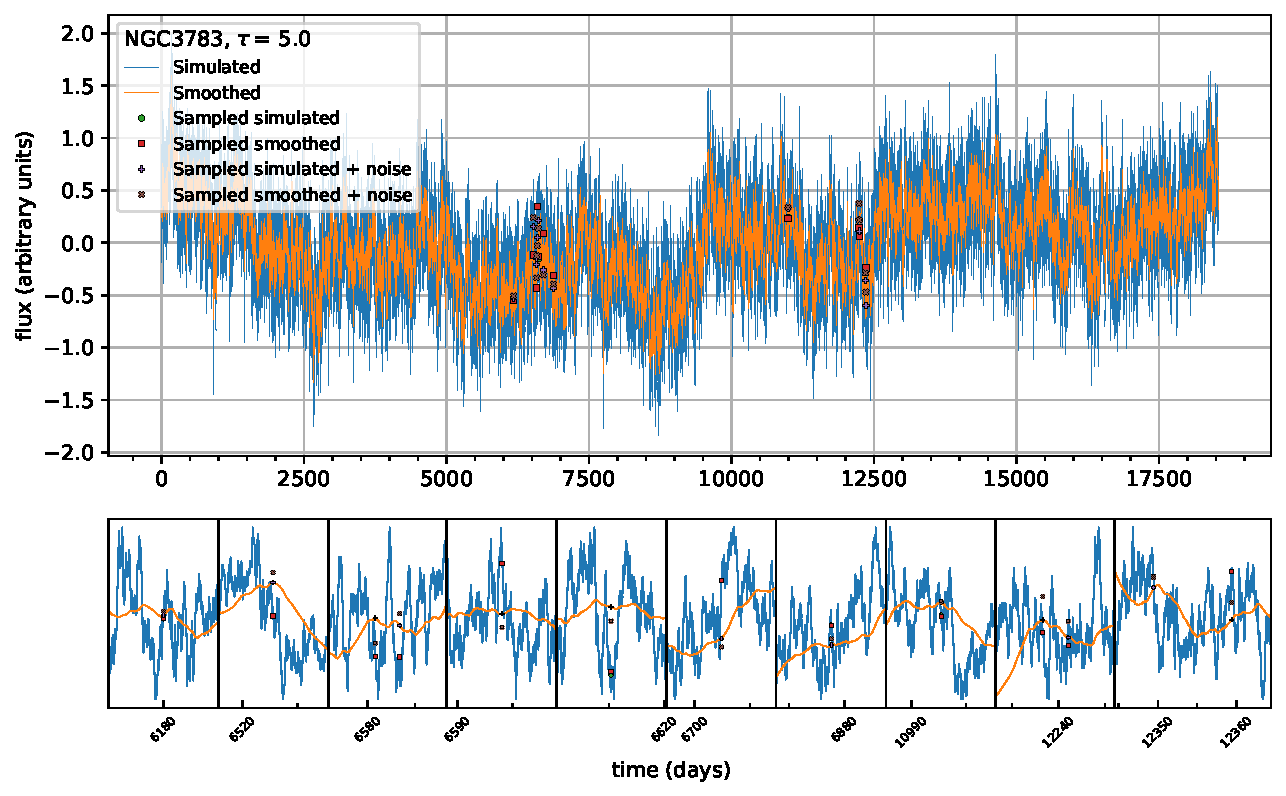
\includegraphics[width=0.49\textwidth]{Figs/Chapter5/NGC3783/sim_LC_tau5.0_0_matrix.pdf} \\
  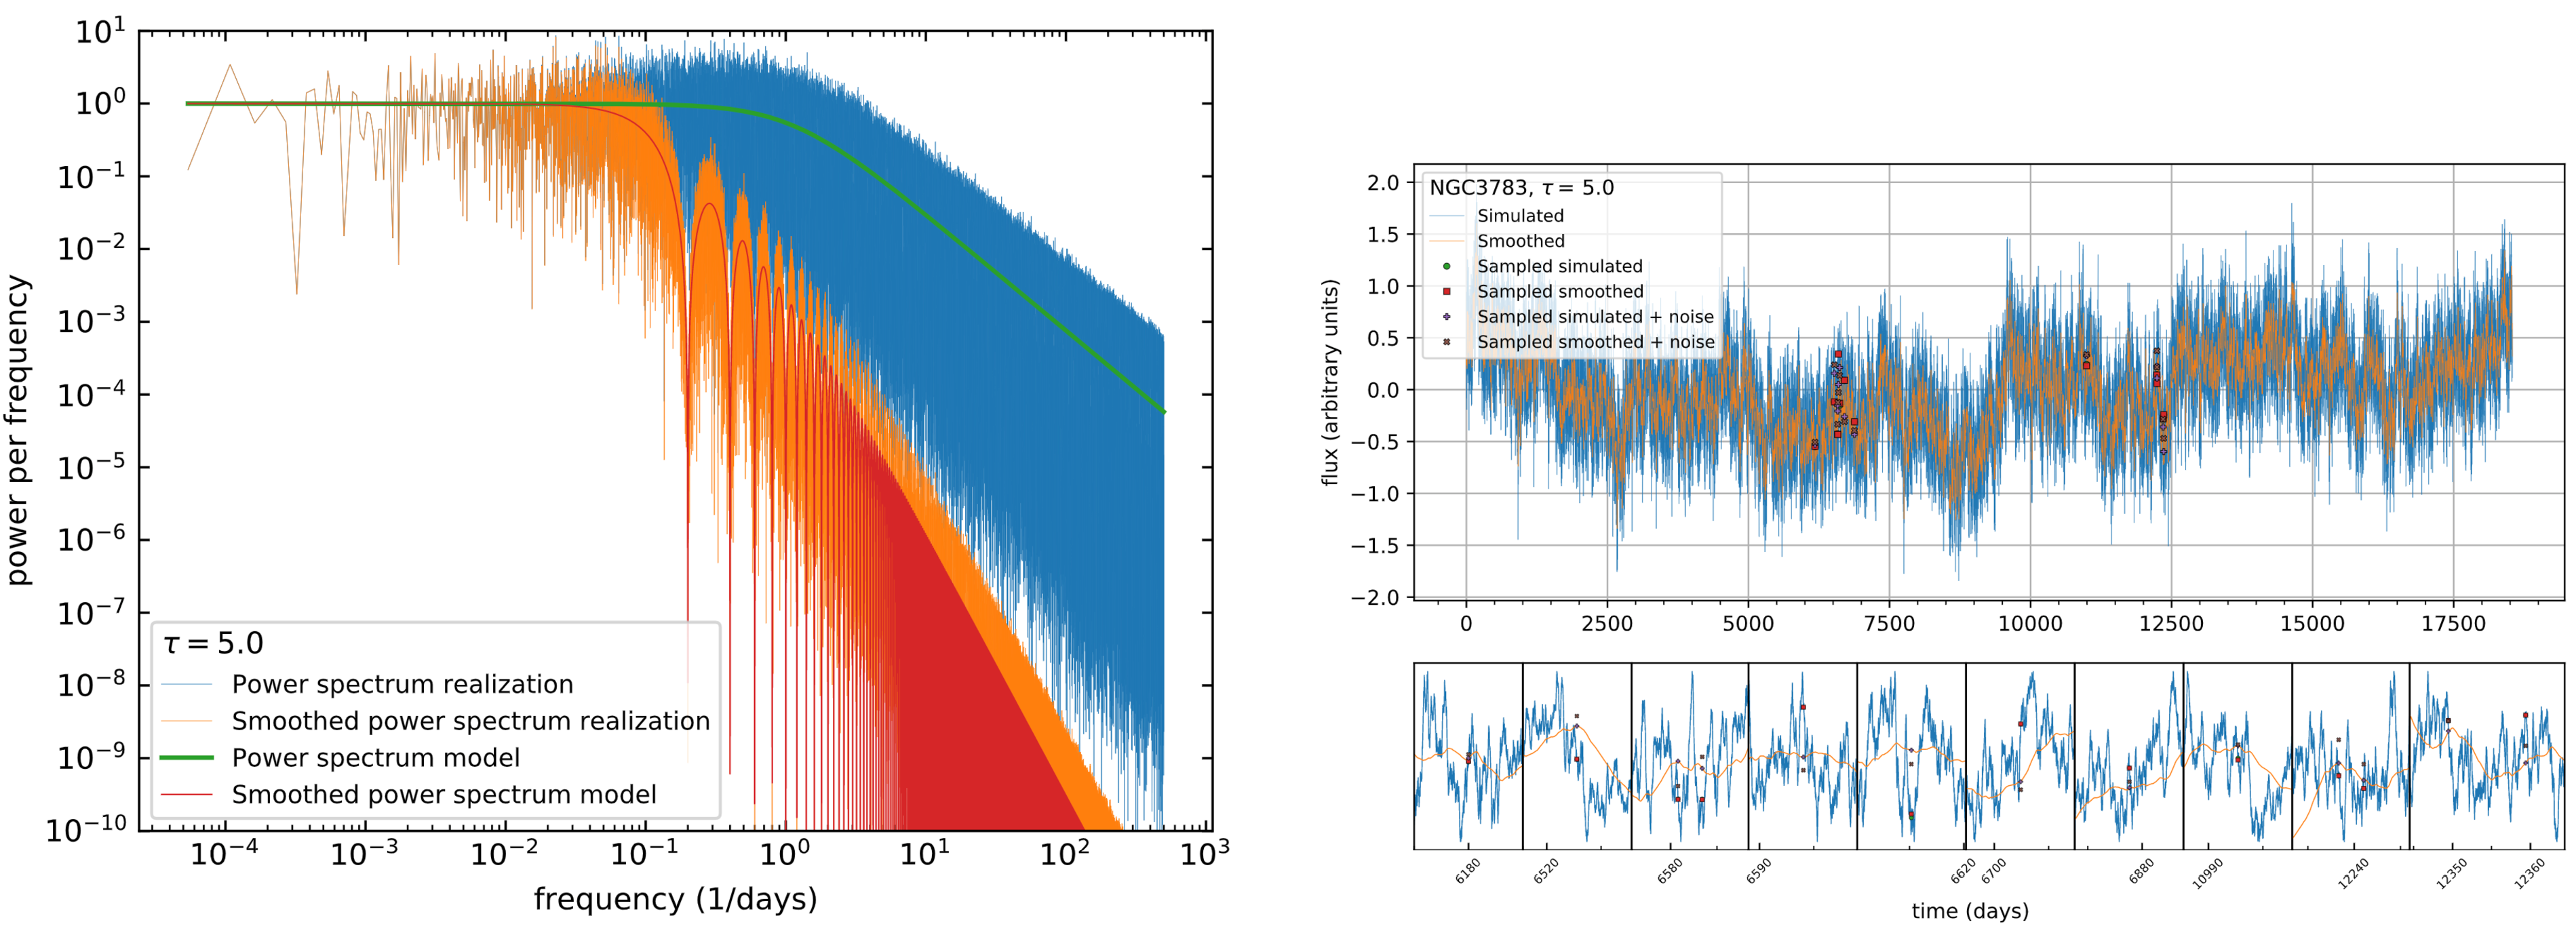
\includegraphics[width=\textwidth]{Figs/Chapter5/NGC3783/Screenshots/NGC3783_tau5_LC_spectrum.pdf} \\
 % 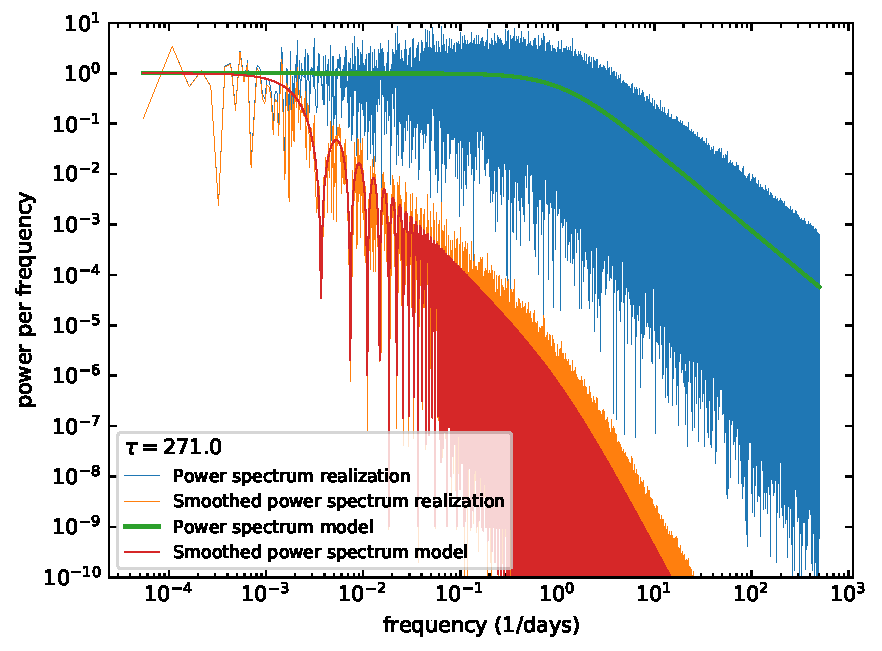
\includegraphics[width=0.49\textwidth]{Figs/Chapter5/NGC3783/power_spectrum_tau271.0.pdf} \hfill 
 % 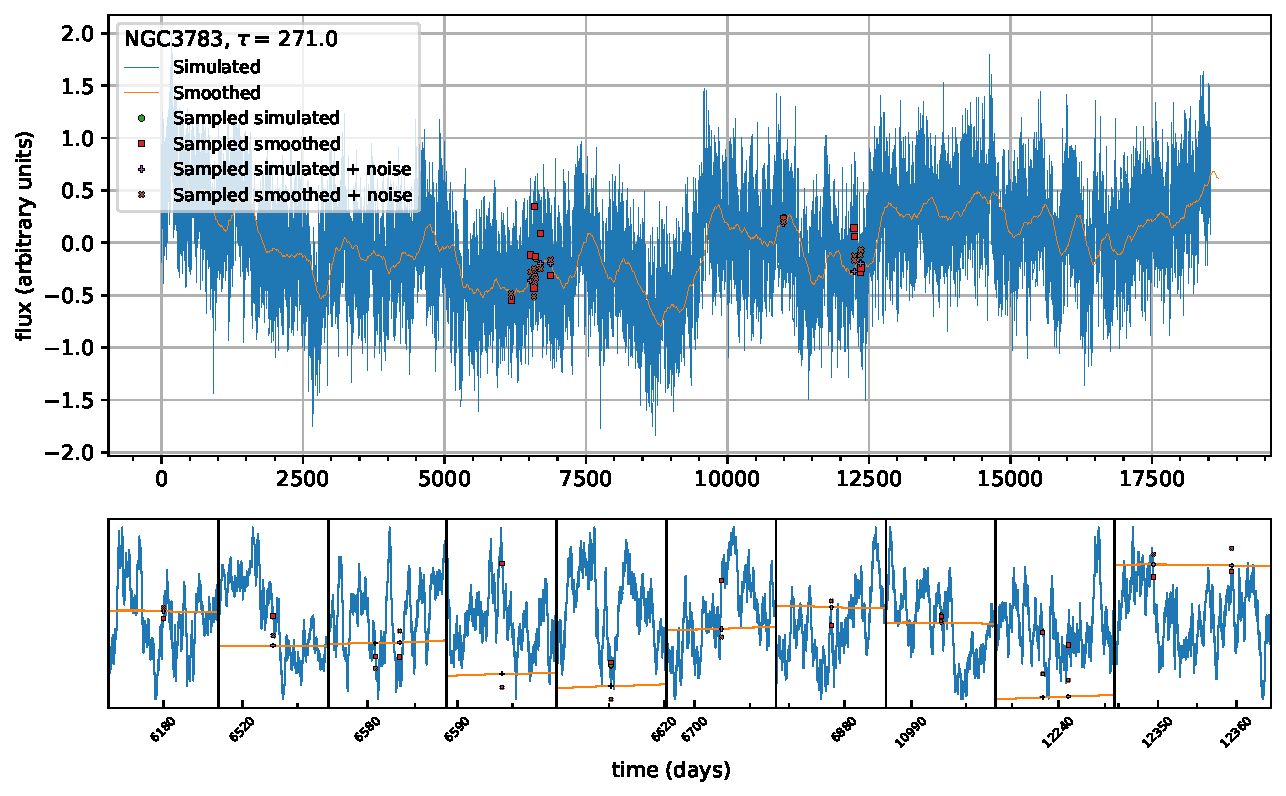
\includegraphics[width=0.49\textwidth]{Figs/Chapter5/NGC3783/sim_LC_tau271.0_0_matrix.pdf} \\
  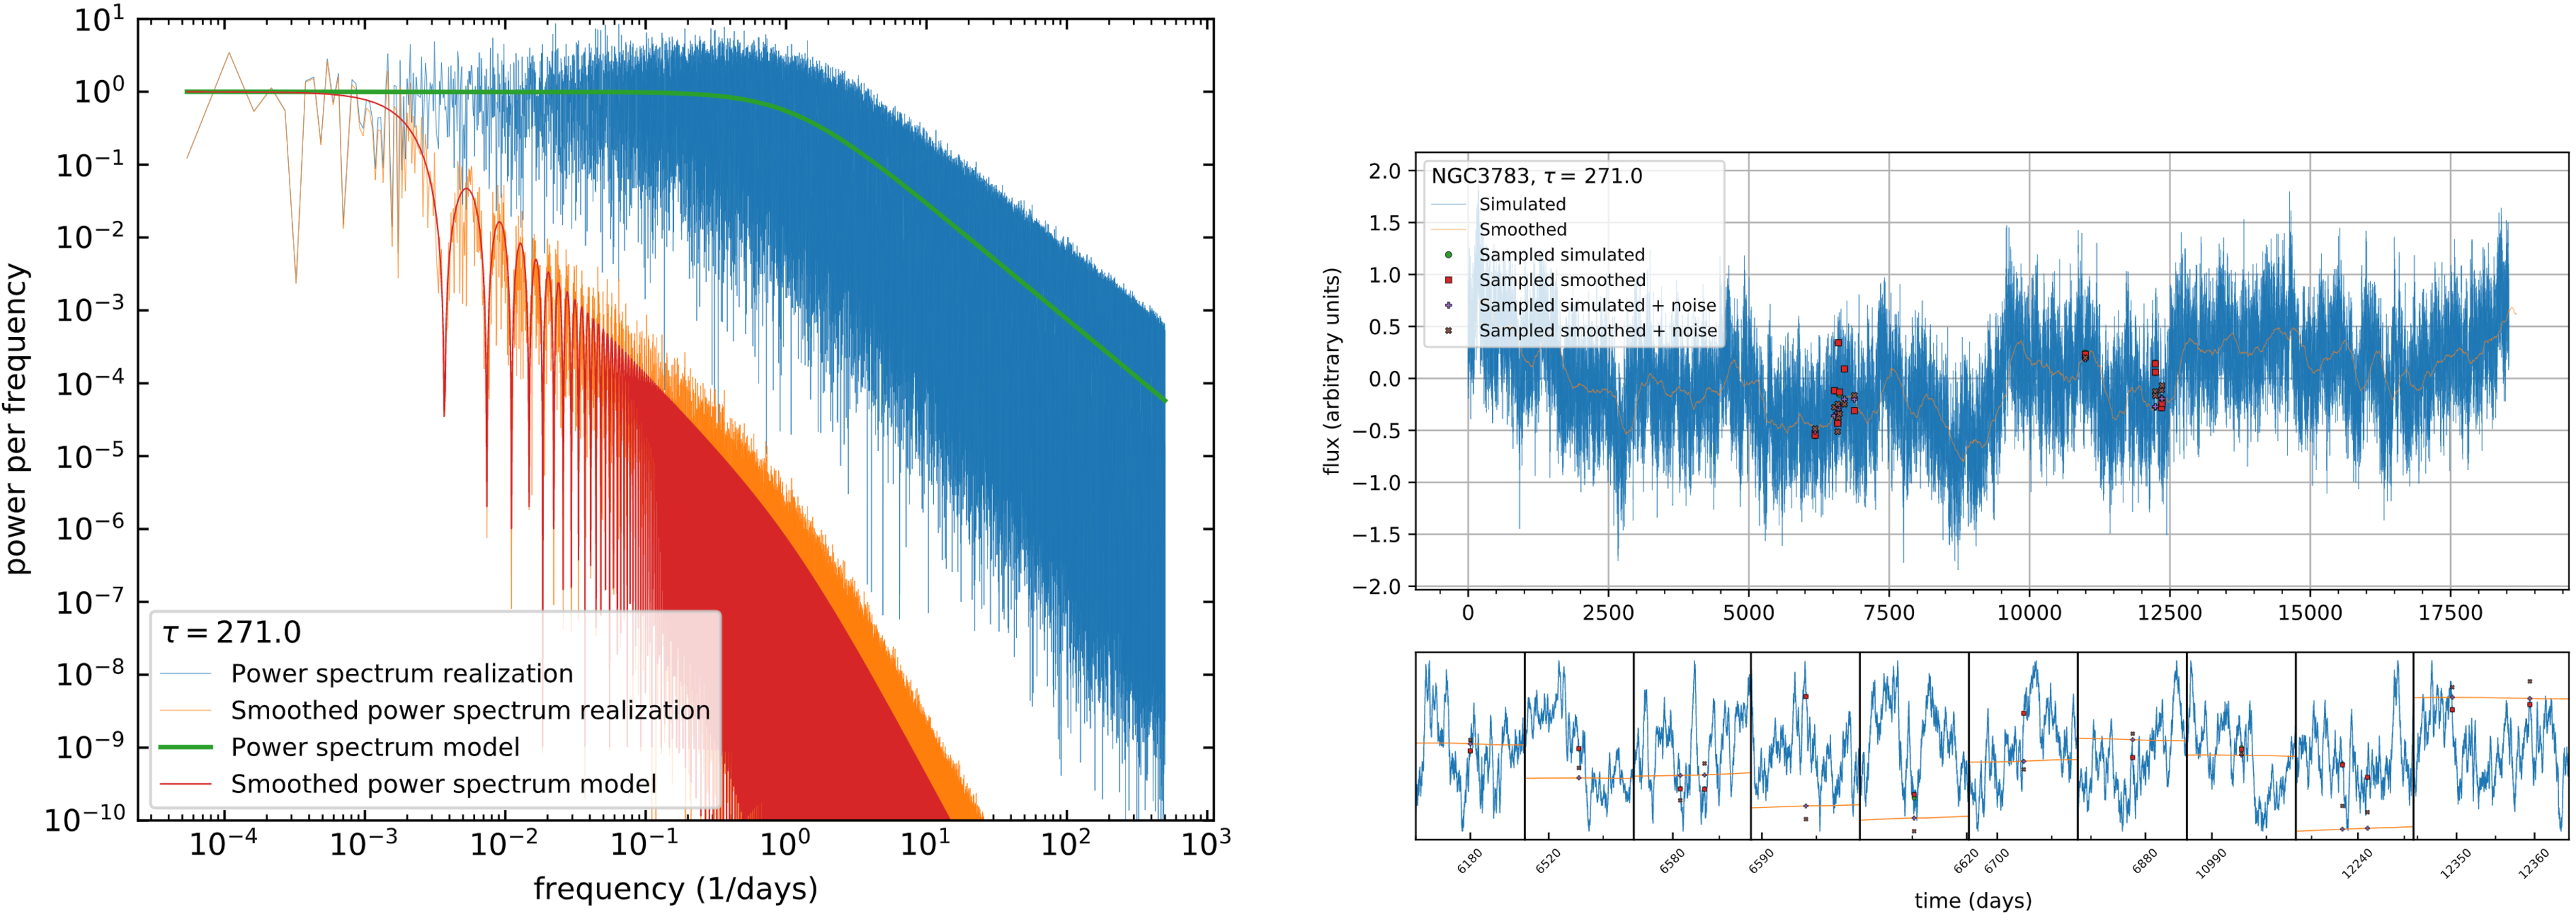
\includegraphics[width=\textwidth]{Figs/Chapter5/NGC3783/Screenshots/NGC3783_tau271_LC_spectrum.pdf} \\
    \label{fig:power_spectra_1_NGC3783}
  }
\end{center}
\end{figure}

\begin{figure}
\begin{center}
    {
 % 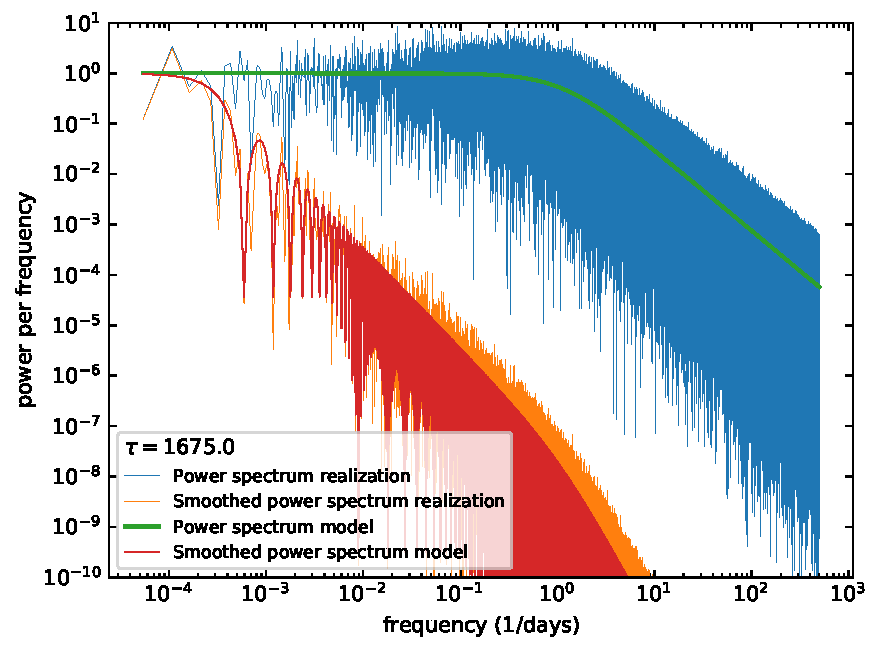
\includegraphics[width=0.49\textwidth]{Figs/Chapter5/NGC3783/power_spectrum_tau1675.0.pdf} \hfill 
 % 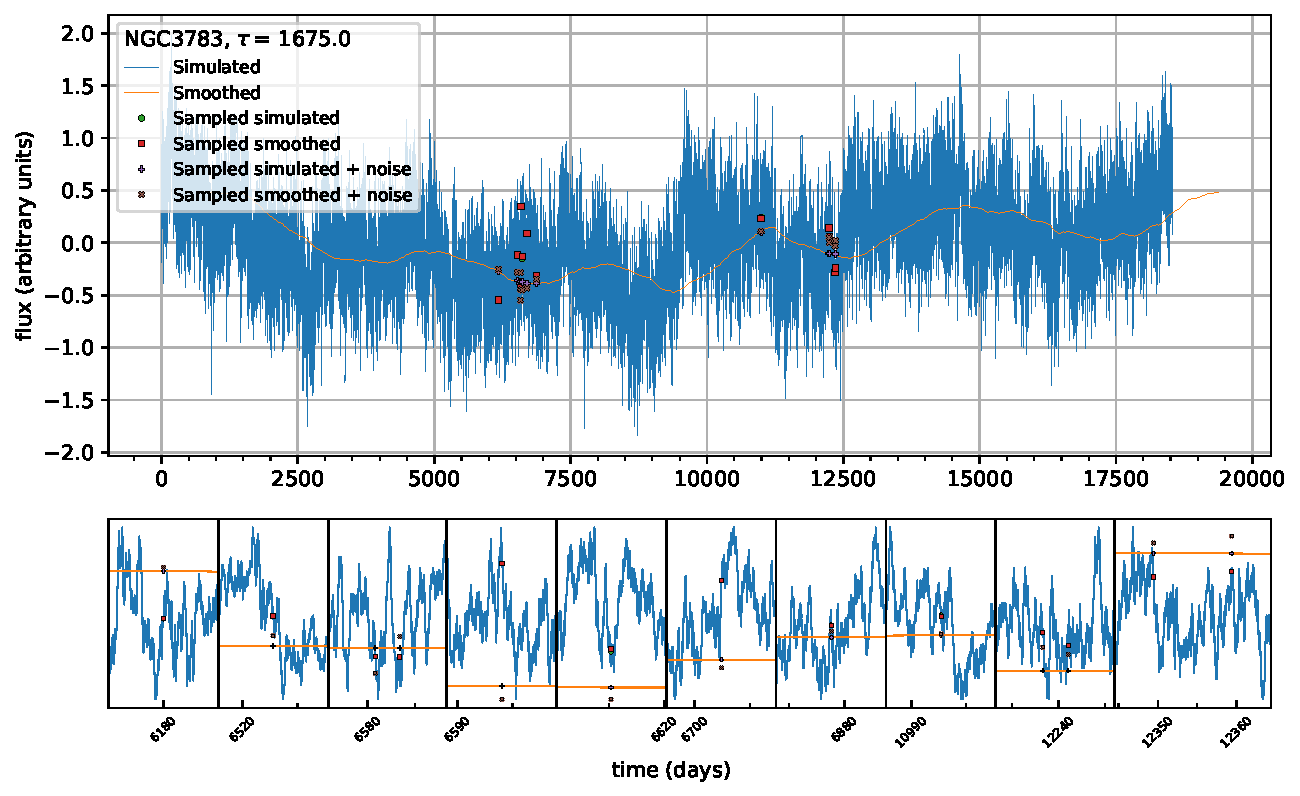
\includegraphics[width=0.49\textwidth]{Figs/Chapter5/NGC3783/sim_LC_tau1675.0_0_matrix.pdf} \\
  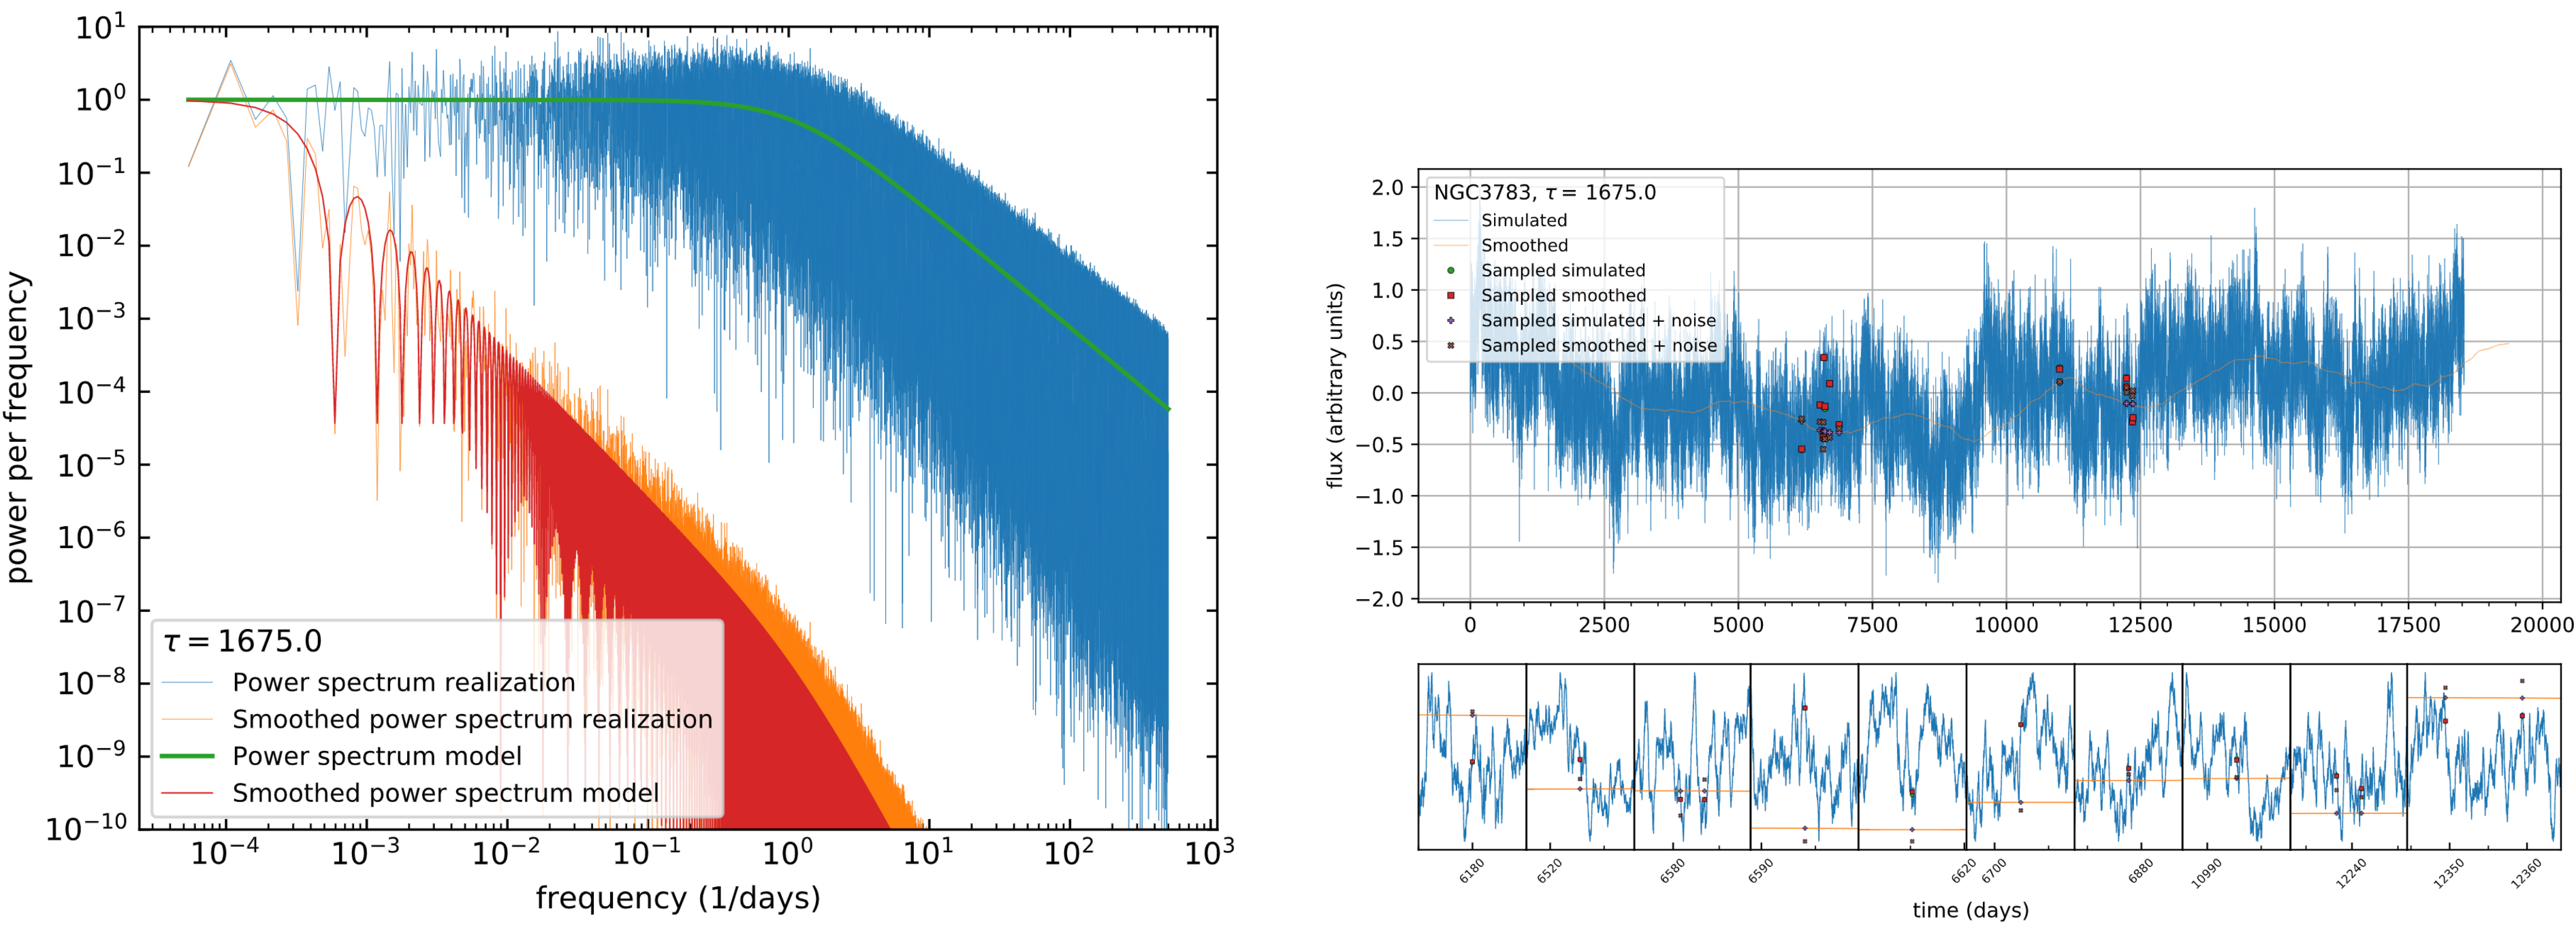
\includegraphics[width=\textwidth]{Figs/Chapter5/NGC3783/Screenshots/NGC3783_tau1675_LC_spectrum.pdf} \\
 % 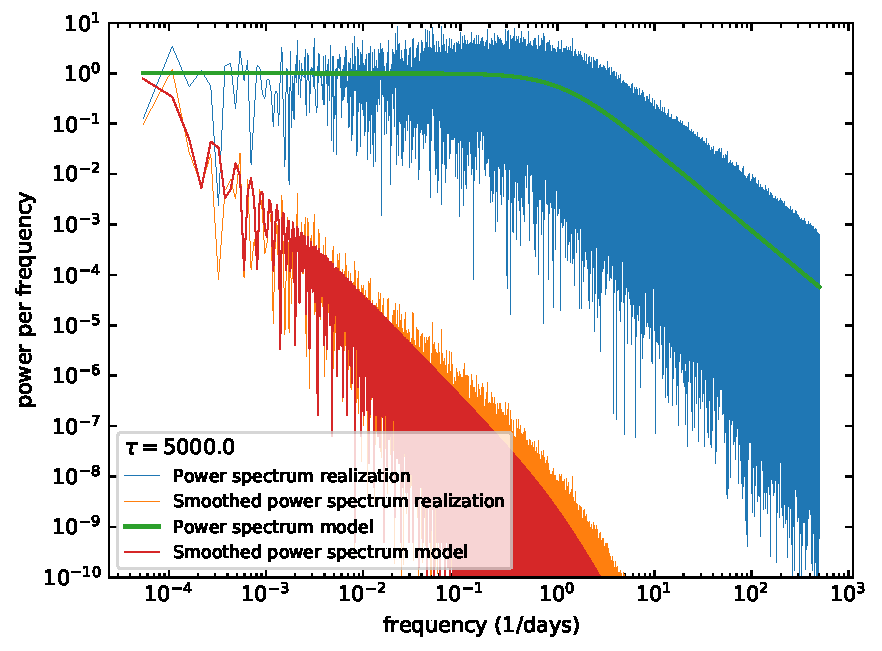
\includegraphics[width=0.49\textwidth]{Figs/Chapter5/NGC3783/power_spectrum_tau5000.0.pdf} \hfill 
 % 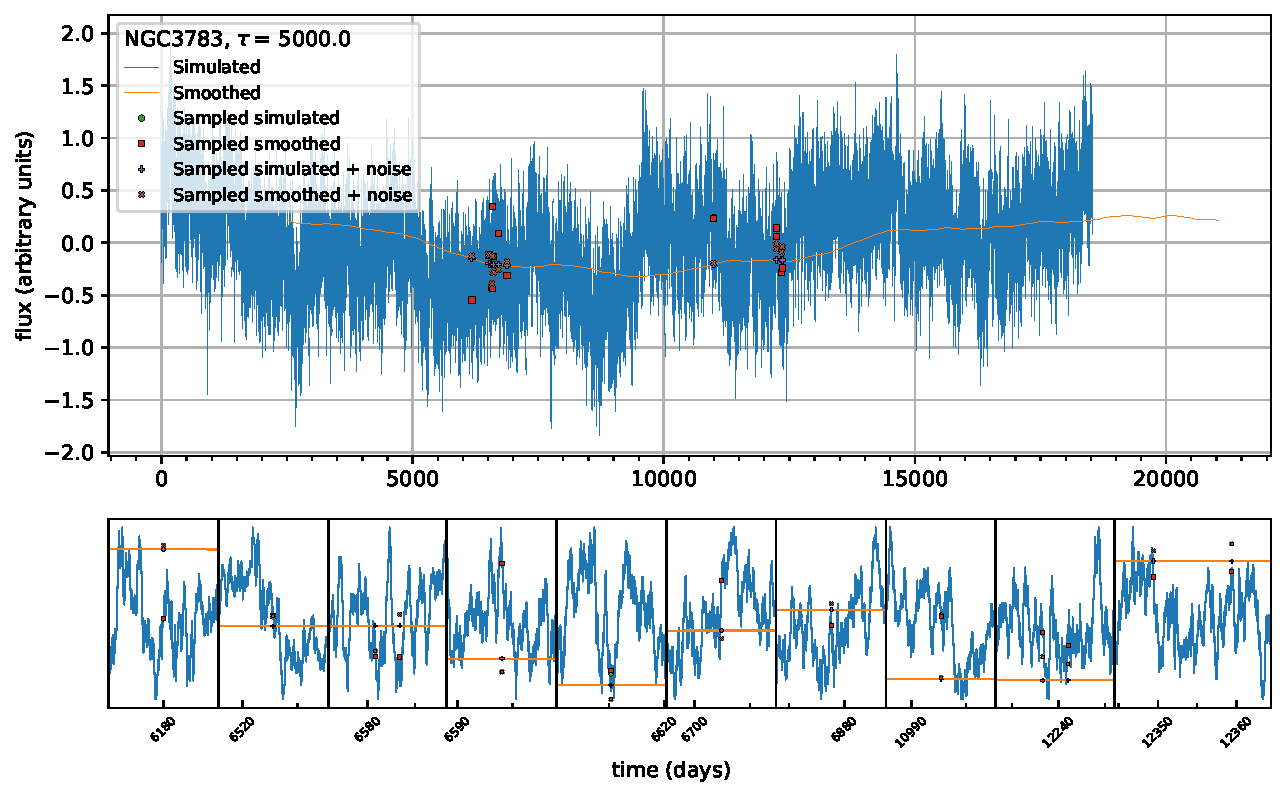
\includegraphics[width=0.49\textwidth]{Figs/Chapter5/NGC3783/sim_LC_tau5000.0_0_matrix.pdf} \\
  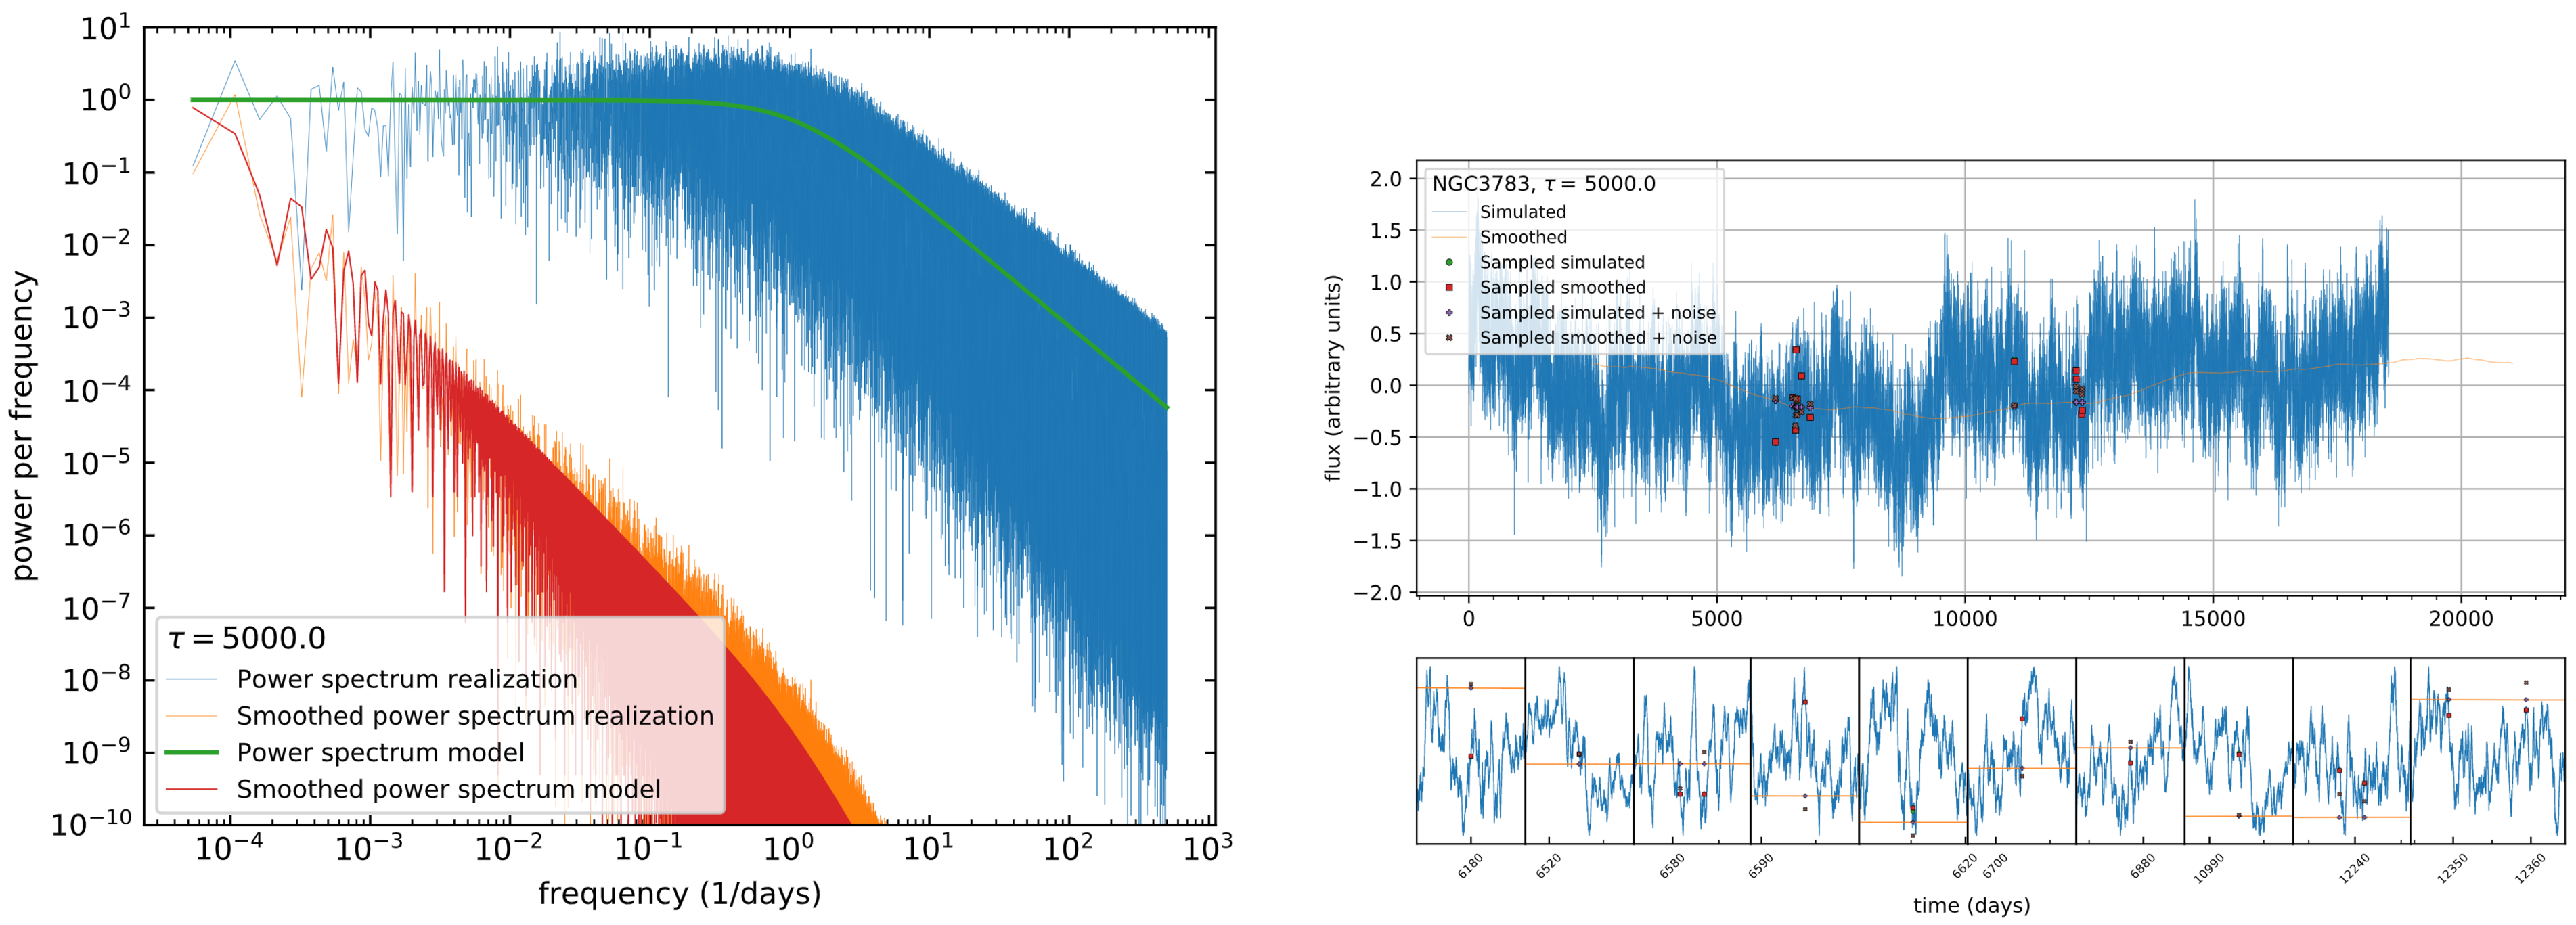
\includegraphics[width=\textwidth]{Figs/Chapter5/NGC3783/Screenshots/NGC3783_tau5000_LC_spectrum.pdf} \\
  \caption{Power spectrum NGC 3783}
    \label{fig:power_spectra_2_NGC3783}
  }
\end{center}
\end{figure}

\begin{figure}
\begin{center}
    {
  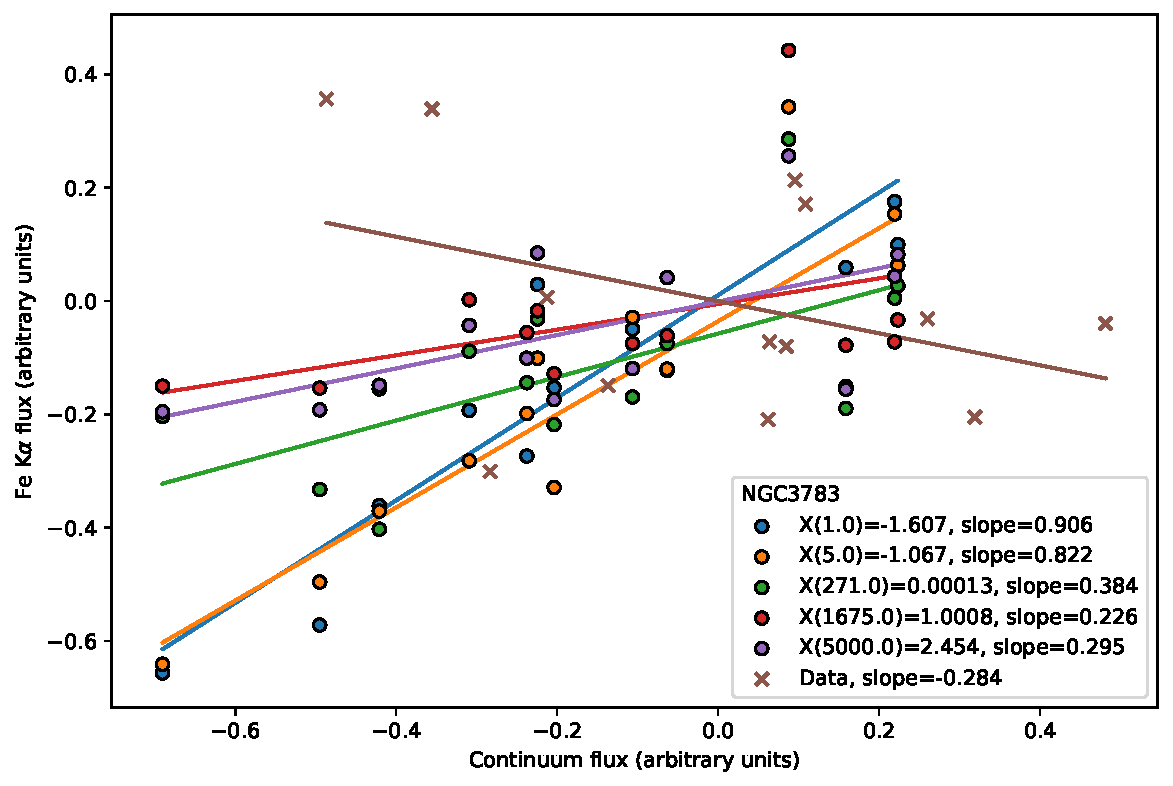
\includegraphics[width=0.7\textwidth]{Figs/Chapter5/NGC3783/Flux_flux_NGC3783.pdf} \hfill 
  \caption{Flux - flux plot NGC 3783}
    \label{fig:Flux-flux_NGC3783}
  }
\end{center}
\end{figure}



\begin{figure}
\begin{center}
    {
  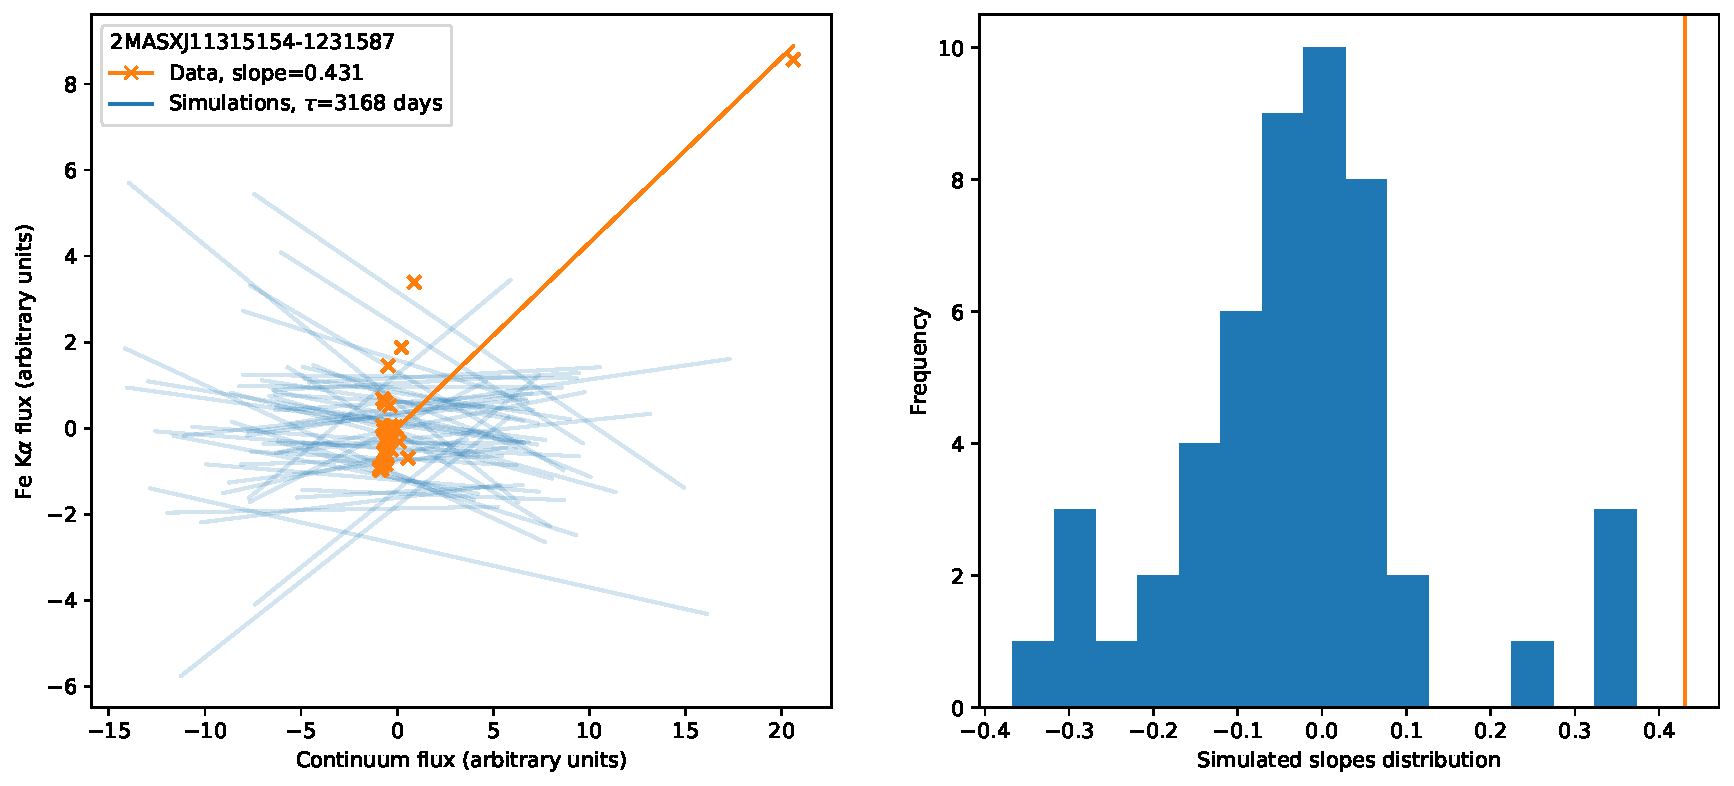
\includegraphics[width=\textwidth]{Figs/Chapter5/Flux_corr/Flux_flux_2MASXJ11315154-1231587_besttau.pdf} \\
  \includegraphics[width=\textwidth]{Figs/Chapter5/Flux_corr/Flux_flux_IC4329A_besttau.pdf} \\
  \includegraphics[width=\textwidth]{Figs/Chapter5/Flux_corr/Flux_flux_MRK1040_besttau.pdf}  \\
  \caption{Flux-flux correlation at best tau}
    \label{fig:Flux-flux_all_1}
  }
\end{center}
\end{figure}

\begin{figure}
\begin{center}
    {
  \includegraphics[width=\textwidth]{Figs/Chapter5/Flux_corr/Flux_flux_MRK273_besttau.pdf} \\
  \includegraphics[width=\textwidth]{Figs/Chapter5/Flux_corr/Flux_flux_MRK290_besttau.pdf} \\
  \includegraphics[width=\textwidth]{Figs/Chapter5/Flux_corr/Flux_flux_MRK509_besttau.pdf}  \\
  \caption{Flux-flux correlation at best tau}
    \label{fig:Flux-flux_all_2}
  }
\end{center}
\end{figure}

\begin{figure}
\begin{center}
    {
  \includegraphics[width=\textwidth]{Figs/Chapter5/Flux_corr/Flux_flux_MRK766_besttau.pdf} \\
  \includegraphics[width=\textwidth]{Figs/Chapter5/Flux_corr/Flux_flux_NGC1275_besttau.pdf} \\
  \includegraphics[width=\textwidth]{Figs/Chapter5/Flux_corr/Flux_flux_NGC1365_besttau.pdf}  \\
  \caption{Flux-flux correlation at best tau}
    \label{fig:Flux-flux_all_3}
  }
\end{center}
\end{figure}

\begin{figure}
\begin{center}
    {
  \includegraphics[width=\textwidth]{Figs/Chapter5/Flux_corr/Flux_flux_NGC2992_besttau.pdf} \\
  \includegraphics[width=\textwidth]{Figs/Chapter5/Flux_corr/Flux_flux_NGC3783_besttau.pdf} \\
  \includegraphics[width=\textwidth]{Figs/Chapter5/Flux_corr/Flux_flux_NGC4151_besttau.pdf}  \\
  \caption{Flux-flux correlation at best tau}
    \label{fig:Flux-flux_all_4}
  }
\end{center}
\end{figure}

\begin{figure}
\begin{center}
    {
  \includegraphics[width=\textwidth]{Figs/Chapter5/Flux_corr/Flux_flux_NGC4388_besttau.pdf} \\
  \includegraphics[width=\textwidth]{Figs/Chapter5/Flux_corr/Flux_flux_NGC7582_besttau.pdf} \\
  \caption{Flux-flux correlation at best tau}
    \label{fig:Flux-flux_all_5}
  }
\end{center}
\end{figure}

\iffalse
Comments:
- light curve time resolution: same number of decimals as \verb+decimals=-int(np.floor(np.log10(abs(1/nu/100))))+ \\
- rescaling    \verb+average_cont = lc['flux_cont(ph/cm^2/s)'].mean()+, 
   \verb+lc['flux_cont(ph/cm^2/s)']=(lc['flux_cont(ph/cm^2/s)']-average_cont)/average_cont+ and same for line (but then I multiply them again for the average....)\\
- explore a range of taus $\tau$, 500 simulations per each \\
- simulated light curve is \verb+n_length*duration+ of the data and is \verb-np.max(taus)/duration+1- if $dt=1e-4$ or \verb+n_length=2+ if $dt=1e-3$ or \verb-max([3,np.max(taus)/duration+1])- if $dt>1e-3$.\\
- Simulation equations, with Re and Im randomly generated numbers with a Gaussian distribution
\begin{equation}
    SimPS_+=(Re+1j*Im)*(PS/2)^{0.5}, \;
    SimPS_-=(Re-1j*Im)*(PS/2)^{0.5}
\end{equation}
- Filter with top hat function in Fourier space, which corresponds to a $\sinc$ function:
- We apply inverse fast Fourier transform (IFFT) to the total SimPS composed of a $0+0j$,$SimPS_+$, and $SimPS_-$. We do the same for SimPSsmooth. \\
- The real part of the result of the two IFFTs is our simulated light curve \\
- Sampling \\
- Noise \\
- Variances - $\xi$ \\
- we want to compare the $\xi_{\rm data}$ with the $\xi_{\rm sim}$ 
- we need to find a $\xi_{\rm sim}$ that matches $\xi_{\rm data}$ such that
\begin{equation}
    {\rm X}(\tau)=\frac{\xi_{\rm data}-<\xi_{\rm sim}>}{(\xi_{\rm sim})_{rms}}=0
\end{equation}
- that tau is the size of the reprocessor\\
- Given how X is defined X$=\pm1$ correspond to $1\sigma$ intervals.\\
- Estimate X \\
- Use Newton's method for finding the root with a tolerance of tol=0.005 and a min time res of 1 day\\
- Run Newton method in order to find also $X=\pm1$ with the same tolerance\\
- Show plots with X of the entire sample
- explain results 
\fi


\section{Discussion}
After constraining the size of the reprocessor for a portion of the galaxies in our sample, we want to find a relation with AGN properties. 
A possibility is for the reprocessor size to scale with the mass of the black hole ${\rm M}_{\rm BH}$. In fact, the size of the circumnuclear environment around the black hole scales with the ${\rm M}_{\rm BH}$, e.g. the Schwarzschild radius, the sphere of influence, etc (?), so it seems viable for the material reprocessing the X-ray emission from the corona to increase its size with ${\rm M}_{\rm BH}$.

If Figure~\ref{fig:tau_mass_corr} we show all the reprocessor sizes in light day units (we remind the reader that the diameter of the reprocessor corresponds to $d=c\tau$), with their uncertainties, as a function of ${\rm M}_{\rm BH}$. Along with these we also show a log-log best fit to the data which shows a slope $0.66\pm0.53$. We see that there is a positive correlation in this relation with a large scatter of $\sim1 dex$.

This seemingly weak correlation though, is an interesting starting point that poses this analysis method as a promising one. In fact it allows to place constraints on the size of the reprocessor of quite a few sources and sets a good base for future monitoring campaigns. In fact, by placing lower limits on the size of the reprocessor we can define good sampling frequencies and by placing upper limits we can define a convenient duration of the monitoring campaign in order to measure the lag between the two light curves. 
Whenever an upper limit is not present, or when this is $\gtrapprox10^3$, it suggests that our kind of analysis based on the measure of the smoothing in the \kalfa{} light curve, is still the best way to go, as very long monitoring campaigns are time expensive and would require years or even decades to lead to a lag measurement. Repeating this analysis with an adequate amount of data-points would certainly allow for a better estimate of the reprocessor size.

%- some galaxies have nuclear reprocessors, others have extended ones

Another possibility for future work is an analysis of the correlation between AGN type properties and $\xi$, as other physical factors may be influencing the emissions and therefore the measured size of the reprocessor, thus causing the scatter in the ${\rm M}_{\rm BH} - \tau$ relation. As already mentioned, the light curves of radio loud sources may be affected from beamed X-ray emission leading to light curves that do not trace the same variations. Another behavior we might expect is from Compton-thick AGN, which should have reflection-dominated continua with little variation, and thus our simple X-ray spectral fitting approach would measure the flux of this relatively static component causing a $\xi<1$. Another example yet is the case of changing look AGN, where covering factor changes may increase the continuum variability from the observers point of view, but not necessarily from the point of view of the whole reflector.
\begin{figure}
\begin{center}
    {
  \includegraphics[width=\textwidth]{Figs/Chapter5/tau_mass_corr.pdf} \hfill 
  \caption{Correlation between black hole mass (${\rm M}_{\rm BH}$) and reprocessor size $\tau$ expressed in light days.}
    \label{fig:tau_mass_corr}
  }
\end{center}
\end{figure}

\section{Conclusions}
In this Chapter we have used simulations in order to study the distribution of X-ray reprocessing gas (\emph{ the reprocessor}) in the active nuclei of a sample of local host galaxies. 
In our simple model we assumed that the X-ray continuum emission comes from the AGN corona and is then reprocessed by a spherical thin shell of gas around it, which causes a delay and a damping of the variations of the continuum in a way that depends on the distance between the corona and the reflector. In order to reproduce the behavior of this setup we simulated the X-ray light curves from the continuum starting from red noise in Fourier space following a power spectrum based on physical parameters of our sources, and the reflected component was obtained from the same light curve, which was smoothed and delayed in time.

The sample in this study was not observed through specific monitoring campaigns aimed at this kind of study, but we used archival data which allowed to retrieve light curves with few data-points observed through several years with irregular sampling. This did not allow to estimate a lag between the light curves but only to determine the variability reduction in amplitude caused by the reprocessor on the reflected component.

This simple modeling allowed us to completely constrain the size of the reprocessor for 4 sources in our sample and to determine at least a lower or upper limit size for 13 of them. For the remaining part of the sample, we either didn't have enough data points to correctly estimate the variability reduction, or the data quality was insufficient, or our model is too simple and does not apply to some individual source. Our resulting reprocessor estimates are still a promising starting point to design future monitoring campaigns that will be more effective at constraining the size of the reprocessor and may even be able to determine a lag between the light curves.

We found a correlation between the size of the reprocessor and the black hole mass ${\rm M}_{\rm BH}$ in our sample, which is consistent with other AGN properties which scale with the mass of the black hole and accretion rate, which include the Schwarzschild radius $r_S$ \citep{1916AbhKP1916..189S}, the internal radius of the dusty torus \citep{2014ApJ...788..159K} and the BLR size \citep{2020MNRAS.491.5881Y}. The relation we found still has large scatter, $\sim1 dex$, which can be in part due to the large uncertainties in our estimation due to few data-points and stochasticity of BH variability but is also probably due to other physical factors like more complex geometries and AGN type dependent imprints that affect our measurements. The variability in the \kalfa{} flux guarantees that the reflector is located in the nuclear surroundings with a size of up to $10^4$ light days, (i.e. $\lesssim10 pc$), since a more extended reflector made of very high column density gas clouds on galactic scales, would imply no visible variability would in the \kalfa{} line flux. The cases in which we were only able to define a lower limit on the reprocessor size may be cases of clouds on galactic scales contributing to the reflection and therefore suggesting a different physical arrangement of the gas.

\clearchapterpage
%%=+=+=+=+=+=+=+=+=+=+=+=+=+=+=+=+=+=+=+=+=+=+=+=+=+=+=+=+=+=+=+=+
%
%%###### Conclusions #######
%%++++++++++++++++++++++++++++++++++++++++++++++++++++++++++++++++
\chapter{Conclusions}

%\begin{center}
%  {\it ``If could add an introductionary text here.''}
%  \vspace{1cm}
%\end{center}

In this thesis we have studied how accretion of the central supermassive black hole evolves in galaxies in all their star formation life phases and through a wide range of cosmic epochs. It is particularly interesting to look for a connection between these two accretion phenomena as they are both fed by cold gas, but they take place on very different galactic scales and it is not clear how the gas can lose angular momentum and funnel into the central black hole, so the two phenomena could in principle be completely independent. We have taken two complementary approaches, we have performed a statistical study on an observational sample from a deep and wide survey, the COSMOS survey, with an exceptional wavelength coverage (Chapter~\ref{ch:observations}), and we have adopted Semi-Empirical models to generate mock galaxy catalogs and thus better understand the physical parameters that shape the relations we found in the data (Chapter~\ref{ch:SEM}).

We have mainly focused on the average ${\rm L}_{\rm X}$ emission of galaxies divided in bins of stellar mass, the ${\rm L}_{\rm X}-{\rm M}_*$ relation, in three galaxy life phases: star forming, quiescent and starburst. We have seen that the ${\rm L}_{\rm X}-{\rm M}_*$ relation, which easily translates into a BHAR$-{\rm M}_*$ relation, follows a decreasing trend in time, probably as less gas is available in galaxies at later cosmic epochs, and that similarly to SFR, starbursts have a higher ${\rm L}_{\rm X}$ than star forming galaxies, and quiescents have a lower ${\rm L}_{\rm X}$. Our SEMs point in the direction that these evolutions in time and across galaxy type are driven by a change in the average Eddington ratio $\zeta_c$ which seems to rule the ${\rm L}_{\rm X}-{\rm M}_*$ normalization. Independent results from observations and models, and also our own from Sec.~\ref{sec:M_vs_M}, suggest that the ${\rm M}_{\rm BH}-{\rm M}_*$ relation is constant with redshift but with a steeper slope than the one that would return our observed ${\rm L}_{\rm X}$ slope, therefore implying an average Eddington ratio $\zeta_c$ decreasing with increasing stellar mass.

We have seen that main-sequence and quiescent galaxies share similar ratios of BHAR and SFR at all probed cosmic epochs, suggesting that the two processes are linked together throughout different galaxy phases. This ratio indicates that at fixed ${\rm M}_{\rm BH}/{\rm M}_*$, a similar BHAR/SFR ratio as the one observed in star forming and quiescent galaxies, would be induced by a proportional decline in characteristic Eddington ratio $\zeta_c$ and specific SFR within a bin of stellar mass. Analogously, the significantly lower BHAR/SFR in starbursts with respect to quiescent/star forming galaxies would be naturally interpreted as a proportionally higher specific SFR and roughly constant or slightly higher $\zeta_c$ in these young, gas rich systems.

Our results on sBHAR and sSFR show similar evolutions and signs of downsizing in all galaxy types and at all explored redshifts, where we define downsizing as the fact that more massive galaxies accreted most of their black hole mass and of the stellar mass at very early cosmic epochs and their accretion decreased fast and steeply, whereas low-mass galaxies have accreted their mass more slowly, but their accretion rate decreased more slowly with time. Downsizing can also be spotted from our mock catalogs from SEMs, that suggest that more massive galaxies have lower characteristic Eddington ratios $\zeta_c$, and is mostly apparent in quiescent galaxies.

Our work points in the direction of a co-evolution of star formation and black hole accretion in galaxies across cosmic time where the bulk of the black hole and stellar masses is accreted in galaxies during the main-sequence phase through secular processes.
Both accretions follow similar evolutionary patterns which appear to be driven by cold gas availability which affects star formation and the characteristic Eddington ratio $\zeta_c$, even though the magnitude of this effect is different in both accretions: the starburst phase seems to be accompanied by a substantial enhancement of the SFR but a limited enhancement of the BHAR, especially at high redshifts. On the other hand, the quiescent phase seems characterized by very little star formation but still a significant residual black hole accretion. The final evolutionary picture that emerges from this work is one in which the host galaxy starts off from a main-sequence or even starburst, gas-rich phase, evolving at an almost constant (specific) SFR and then gradually switches off its black hole accretion and star formation due to internal gas consumption, thus gradually reducing the SFR and BHAR.

\vspace{10pt}
On a distinct approach, in Chapter~\ref{ch:gas_distribution} we have studied the gas distribution around the AGN by simulating the variability of X-ray emissions from the corona and from the reprocessing gas in a sample of local galaxies. We used a simple model which assumed the reprocessing gas to be arranged in a spherical thin shell around the active galactic nucleus, which acts by delaying and smoothing out the variations of the continuum emission from the corona. This very simple model, together with sparse light curves from archival data allowed to place constraints for 17 out of 33 sources, constraints which could be useful in order to design future monitoring surveys. We also found a correlation with a large scatter between the size of the reprocessing gas and the mass of the black hole, suggesting that the mass of the BH plays a role in defining the gas arrangement around it, but also that our model may be too simple for some of our galaxies, and that the size of the reprocessor could depend on other physical factors like more complex geometries and/or AGN type dependent emission imprints. 
\clearchapterpage
%%=+=+=+=+=+=+=+=+=+=+=+=+=+=+=+=+=+=+=+=+=+=+=+=+=+=+=+=+=+=+=+=+

\appendix

%###### APPENDIX 1 #######
%=+=+=+=+=+=+=+=+=+=+=+=+=+=+=+=+=+=+=+=+=+=+=+=+=+=+=+=+=+=+=+=+
%====   FINITO ====
%++++++++++++++++++++++++++++++++++++++++++++++++++++++++++++++++
%\appendix
%{\bfseries \huge Constraining torus models for AGN using X-ray observations}

\chapter{Chapter~\ref{ch:observations} additional data}

%\begin{center}
%  {\it ``You could put an introductionary text here''} \\
%  \vspace{1cm}
%\end{center}

\section{Sample properties} \label{appendix_observations}
We report the Tables with additional properties of our galaxy sample from Chapter~\ref{ch:observations}. Table~\ref{tab:SF_prop} lists star-forming galaxies, Table~\ref{tab:Q_prop}  quiescent galaxies, and Table~\ref{tab:SB_prop} starbursts.

\begin{table*}\centering
\caption{Properties of the star-forming galaxy sample. For each mass and redshift bin we show the median mass and redshift, and the number of stacked and detected galaxies in the 2-7~keV band.
We also show the X-ray luminosity, the SFR estimated from the FIR, and the obscured SFR from the UV. Quantities are medians, and confidence ranges are 1$\sigma$.}
\vspace{5pt}
\label{tab:SF_prop}
%\resizebox{1\textwidth}{!}{
\begin{tabular}{lc|c|c c|c c c}
%\begin{tabular}{lc|c|c c|c c c|c c | c c}
\hline
\hline
$\text{Mass range}$                             & $M_*$ &  $z$  & N$_{\text{stacked}}$  & N$_{\text{detected}}$ & $L_{\text{2-10~keV}}$   & $\text{SFR}_{IR}$ & $\text{SFR}_{UV}$  \\     %& $\frac{\text{L}_{\text{SF}}}{<\text{L}_{\text{tot}}>}$\tiny{(2-10keV)}       & <BHAR>  & <M$_\text{BH}$>       & <sBHAR>       & <sSFR> \T \\
$\log_{10}($M$_*$/M$_\sun)$     & $\log_{10}($M$_*$/M$_\sun)$   & &     &                       & $10^{42}\um{erg}\ump{s}{-1}$    & M$_\odot \ump{yr}{-1}$        & M$_\odot \ump{yr}{-1}$\\ %& & &  \T \B \\
\hline
\hline
\multicolumn{8}{l}{$0.10<z<0.65$}       \\
\hline
9.5--10.0               &  9.72    & 0.46       & 4244  & 19    & $0.023^{+0.007}_{-0.007}$     & $ 2.22^{+0.08}_{-0.07}$ & $0.500^{+0.012}_{-0.011}$             \T \B \\    
10.0--10.5          & 10.21    & 0.45   & 2514  & 75    & $0.142^{+0.009}_{-0.009}$     & $ 5.68^{+2.67}_{-0.17}$ & $0.479^{+0.013}_{-0.018}$             \T \B \\     
10.5--11.0              & 10.70    & 0.45       & 1214  & 117   & $0.639^{+0.015}_{-0.015}$     & $14.2 ^{+0.7 }_{-0.7 }$ & $0.56 ^{+0.03 }_{-0.02 }$             \T \B \\      
11.0--12.0          & 11.14    & 0.43   & 239   & 38    & $1.550^{+0.038}_{-0.036}$     & $15.7 ^{+2.2 }_{-2.4 }$ & $0.76 ^{+0.07 }_{-0.11 }$             \T \B \\       
\hline
\hline
\multicolumn{8}{l}{$0.65<z<1.30$}        \\
\hline
9.5--10.0               &  9.72   & 0.97        & 15431 & 56    & $ 0.15^{+0.02}_{-0.02} $       & $ 4.70^{+0.14}_{-0.13}$       & $1.051^{+0.009}_{-0.011} $    \T \B \\   
10.0--10.5          & 10.22   & 0.97    & 7957  & 175   & $ 0.66^{+0.03}_{-0.03} $       & $14.9 ^{+0.3 }_{-0.3 }$       & $0.854^{+0.018}_{-0.015} $    \T \B \\   
10.5--11.0              & 10.69   & 0.95        & 3888  & 370   & $ 2.67^{+0.05}_{-0.05} $       & $26.8 ^{+0.5 }_{-0.5 }$       & $0.856^{+0.023}_{-0.016} $    \T \B \\   
11.0--12.0          & 11.15   & 0.95    & 761   & 142   & $ 5.13^{+0.12}_{-0.12} $       & $37.1 ^{+2.7 }_{-2.1 }$       & $1.29 ^{+0.08 }_{-0.13 } $    \T \B \\   
\hline
\hline
\multicolumn{8}{l}{$1.30<z<2.25$}        \\
\hline                  
9.5--10.0               &  9.80    & 1.64       & 13451 & 47    & $ 0.35^{+0.09}_{-0.08} $       & $10.4^{+0.6}_{-0.6}$          & $2.17^{+0.02 }_{-0.02} $      \T \B \\   
10.0--10.5          & 10.22    & 1.73   & 11334 & 177   & $ 1.47^{+0.09}_{-0.10} $       & $30.2^{+0.7}_{-0.7}$          & $1.62^{+0.03 }_{-0.03} $      \T \B \\   
10.5--11.0              & 10.69    & 1.74       & 5273  & 368   & $ 5.97^{+0.17}_{-0.16} $       & $57.0^{+1.5}_{-1.5}$          & $1.18^{+0.02 }_{-0.02} $      \T \B \\   
11.0--12.0          & 11.12    & 1.76   & 954   & 172   & $18.21^{+0.43}_{-0.45} $       & $97.0^{+4.6}_{-4.7}$          & $1.46^{+0.04 }_{-0.06} $      \T \B \\   
\hline
\hline
\multicolumn{8}{l}{$2.25<z<3.50$}        \\
\hline
9.5--10.0               &  9.92    & 2.69       & 1264  & 3         & $  0.8^{+0.8 }_{-0.9} $    & $ 14.9^{+ 8.6}_{- 6.7}$       & $4.72^{+0.15}_{-0.17} $        \T \B \\  
10.0--10.5          & 10.22        & 2.77       & 7159  & 98    & $  2.9^{+0.4 }_{-0.4} $      & $ 68.2^{+ 4.4}_{- 4.1}$       & $4.49^{+0.07}_{-0.08} $        \T \B \\  
10.5--11.0              & 10.68    & 2.73       & 2726  & 166   & $ 14.9^{+0.6 }_{-0.6} $   & $139.4^{+ 9.1}_{- 9.1}$  & $2.78^{+0.06}_{-0.05} $        \T \B \\  
11.0--12.0          & 11.13        & 2.69       & 466   & 70    & $ 35.5^{+1.6 }_{-1.5} $   & $243.4^{+16.3}_{-14.8}$  & $2.44^{+0.12}_{-0.14} $        \T \B \\  
\hline

\end{tabular}%  }
\end{table*}
%
%%%%%%%%%%%%%%%%%%%%%%%%%%%%%%%%%%%%%%%%%%%%%%%%%%%%%%%%%%%%%%
\begin{table*}\centering
\caption{Same as Table~\ref{tab:SF_prop} for the quiescent galaxy sample.}
\vspace{5pt}
\label{tab:Q_prop}
%\resizebox{1\textwidth}{!}{
\begin{tabular}{lc|c|c c|c c c}
%\begin{tabular}{lc|c|c c|c c c|c c | c c}
\hline
\hline
$\text{Mass range}$                             & $M_*$ &  $z$  & N$_{\text{stacked}}$  & N$_{\text{detected}}$ & $L_{\text{2-10~keV}}$   & $\text{SFR}_{IR}$ & $\text{SFR}_{UV}$  \\     %& $\frac{\text{L}_{\text{SF}}}{<\text{L}_{\text{tot}}>}$\tiny{(2-10keV)}       & <BHAR>  & <M$_\text{BH}$>       & <sBHAR>       & <sSFR> \T \\
$\log_{10}($M$_*$/M$_\sun)$     & $\log_{10}($M$_*$/M$_\sun)$   & &     &                       & $10^{42}\um{erg}\ump{s}{-1}$    & M$_\odot \ump{yr}{-1}$        & M$_\odot \ump{yr}{-1}$\\ %& & &  \T \B \\
\hline
\hline
\multicolumn{8}{l}{$0.10<z<0.65$}       \\
\hline
10.0--10.5          & 10.27    & 0.47   & 867   & 12    & $0.060^{+0.017}_{-0.018}$     & $0.40^{+0.07}_{-0.09}$  & $0.017^{+0.002}_{-0.002}$       \T \B \\ 
10.5--11.0              & 10.74    & 0.47       & 830   & 19    & $0.061^{+0.018}_{-0.015}$     & $0.51^{+0.12}_{-0.10}$  & $0.026^{+0.004}_{-0.004}$       \T \B \\ 
11.0--12.0          & 11.16    & 0.50   & 271   & 14    & $0.177^{+0.035}_{-0.035}$     & $0.96^{+0.21}_{-0.22}$  & $0.074^{+0.010}_{-0.017}$       \T \B \\ 
\hline
\hline
\multicolumn{8}{l}{$0.65<z<1.30$}        \\
\hline
10.0--10.5          & 10.30   & 0.93    & 2594  & 19    & $0.18^{+0.04}_{-0.05}$        & $1.3 ^{+0.3 }_{-0.4 }$  & $0.083^{+0.002}_{-0.002}$     \T \B \\   
10.5--11.0              & 10.75   & 0.94        & 3354  & 72    & $0.41^{+0.04}_{-0.04}$        & $2.2 ^{+0.3 }_{-0.2 }$  & $0.130^{+0.003}_{-0.004}$     \T \B \\   
11.0--12.0          & 11.15   & 0.93    & 1107  & 25    & $0.47^{+0.08}_{-0.08}$        & $2.8 ^{+0.5 }_{-0.4 }$  & $0.172^{+0.009}_{-0.010}$     \T \B \\   
\hline
\hline
\multicolumn{8}{l}{$1.30<z<2.25$}        \\
\hline                  
10.0--10.5          & 10.25    & 1.58   & 769   & 9     & $0.6^{+0.3}_{-0.3}$           & $- $                                            & $0.279^{+0.013}_{-0.011}$     \T \B \\   
10.5--11.0              & 10.75    & 1.57       & 1534  & 25    & $1.2^{+0.2}_{-0.2}$           & $7.4^{+0.8}_{-0.8}$             & $0.307^{+0.008}_{-0.008}$     \T \B \\   
11.0--12.0          & 11.14    & 1.59   & 532   & 8     & $1.8^{+0.4}_{-0.4}$           & $6.0^{+2.1}_{-3.0}$             & $0.400^{+0.021}_{-0.012}$     \T \B \\   
\hline
\hline
\multicolumn{8}{l}{$2.25<z<3.50$}        \\
\hline
10.0--10.5          & 10.32        & 2.56       & 105   & 3         & $ 8.4^{+2.5}_{-2.6}$          & $- $                                               & $1.25^{+0.22}_{-0.06}$        \T \B \\  
10.5--11.0              & 10.75    & 2.52       & 272   & 7     & $ 2.6^{+1.5}_{-1.5}$      & $- $                                             & $1.15^{+0.06}_{-0.07}$        \T \B \\  
11.0--12.0          & 11.12        & 2.48       & 66    & 6         & $22.2^{+3.6}_{-3.6}$      & $-$                                              & $1.71^{+0.18}_{-0.15}$        \T \B \\  
\hline
\end{tabular}%  }
\end{table*}
  %
%%%%%%%%%%%%%%%%%%%%%%%%%%%%%%%%%%%%%%%%%%%%%%%%%%%%%%%%%%%%%%
\begin{table*}\centering
\caption{Same as Table~\ref{tab:SF_prop} for the starburst galaxy sample. We only use SFR$_{IR}$ for this sample.}
\vspace{5pt}
\label{tab:SB_prop}
%\resizebox{1\textwidth}{!}{
\begin{tabular}{lc|c|c c|c c}
%\begin{tabular}{lc|c|c c|c c c|c c | c c}
\hline
\hline
$\text{Mass range}$                             & $M_*$ &  $z$  & N$_{\text{stacked}}$  & N$_{\text{detected}}$ & $L_{\text{2-10~keV}}$   & $\text{SFR}_{IR}$  \\ %& $\text{SFR}_{UV}$ & $\frac{\text{L}_{\text{SF}}}{<\text{L}_{\text{tot}}>}$\tiny{(2-10keV)}      & <BHAR>  & <M$_\text{BH}$>       & <sBHAR>       & <sSFR> \T \\
$\log_{10}($M$_*$/M$_\sun)$     & $\log_{10}($M$_*$/M$_\sun)$   & &     &               & $10^{42}\um{erg}\ump{s}{-1}$    & M$_\odot \ump{yr}{-1}$        \\ %& M$_\odot \ump{yr}{-1}$& & &      \T \B \\
\hline
\hline
\multicolumn{7}{l}{$0.10<z<0.65$}\\
\hline
9.50--10.25          &  9.87    & 0.53 & 58 & 4     & $0.36^{+0.09}_{-0.09}$  & $ 22^{+ 4}_{- 2}$    \T \B \\
10.25--10.75     & 10.52        & 0.53 & 6  & 5         & $4.68^{+0.40}_{-0.41}$  & $ 74^{+20}_{- 9}$    \T \B \\
10.75--11.50     & 10.96        & 0.52 & 2  & 3         & $6.64^{+0.67}_{-0.68}$  & $143^{+ 5}_{- 1}$    \T \B \\
\hline                                                                                     
\hline                                                                                     
\multicolumn{7}{l}{$0.65<z<1.30$} \\  
\hline                                 
9.50--10.25              &  9.90        & 0.95 & 162 & 7        & $0.8^{+0.2}_{-0.2}$    & $ 66^{+ 3}_{- 3}$     \T \B \\
10.25--10.75     & 10.42        & 1.04 & 161 & 10       & $2.5^{+0.3}_{-0.3}$          & $131^{+ 5}_{- 2}$    \T \B \\
10.75--11.50     & 10.91        & 1.08 & 43  & 5        & $6.2^{+0.6}_{-0.6}$    & $280^{+15}_{-16}$     \T \B \\
\hline
\hline
\multicolumn{7}{l}{$1.30<z<2.25$}\\
\hline                                                                                           
9.50--10.25              & 10.01        & 1.76 & 57  & 1        & $-$                    & $222^{+15}_{-18}$     \T \B \\
10.25--10.75     & 10.50        & 1.74 & 145 & 24       & $15.1^{+1.2}_{-1.2}$   & $331^{+16}_{- 9}$     \T \B \\
10.75--11.50     & 10.89        & 1.79 & 78  & 23       & $40.8^{+2.0}_{-2.0}$   & $536^{+34}_{-23}$     \T \B \\
\hline 
\hline
\multicolumn{7}{l}{$2.25<z<3.50$}\\  
\hline                                                                                   
9.50--10.25              & 10.07        & 2.48  & 5   & 0   & $-$                        & $ 384^{+ 14}_{- 41}$  \T \B \\
10.25--10.75     & 10.53        & 2.59  & 64  & 2       & $ 8.3^{+4.5}_{-4.1}$   & $ 739^{+ 27}_{- 26}$ \T \B \\
10.75--11.50     & 10.90        & 2.68  & 46  & 7   & $20.1^{+5.5}_{-5.3}$       & $1229^{+148}_{-139}$ \T \B \\
\hline
\end{tabular}%  }
\end{table*}
  

\clearchapterpage
%=+=+=+=+=+=+=+=+=+=+=+=+=+=+=+=+=+=+=+=+=+=+=+=+=+=+=+=+=+=+=+=+

%
% Add as many appendixes as you want
%
%%###### APPENDIX 2 #######
%%=+=+=+=+=+=+=+=+=+=+=+=+=+=+=+=+=+=+=+=+=+=+=+=+=+=+=+=+=+=+=+=+
%%====   FINITO ====
%%++++++++++++++++++++++++++++++++++++++++++++++++++++++++++++++++
%\include{FCCAp2}
%\clearchapterpage
%%=+=+=+=+=+=+=+=+=+=+=+=+=+=+=+=+=+=+=+=+=+=+=+=+=+=+=+=+=+=+=+=+


\bibliographystyle{mnras}
\bibliography{12-references}


\end{document}
